\documentclass[a4paper,adobefonts,11pt,UTF8]{book}

\usepackage{ctex}
\usepackage{makeidx}
\usepackage[headheight=13.6pt]{geometry}
\usepackage{fontspec}
\usepackage{xunicode}
\usepackage{xltxtra}
\usepackage{amsmath}
\usepackage{amssymb}

\graphicspath{{../img/}}

\usepackage{verbatim}
\usepackage{graphicx}
\usepackage{multirow}

\usepackage[svgnames,table]{xcolor}
\usepackage{paralist}
\usepackage{longtable}
\usepackage{ulem}
%\usepackage{rotating}
\usepackage{color,colortbl}



\usepackage{listings}
\lstset{
	basicstyle=\ttfamily,
	showstringspaces=false,
	commentstyle=\color{red},
	keywordstyle=\color{blue},
	columns=flexible
}

\usepackage{bashful}

\usepackage[bookmarksnumbered,pdfencoding=auto,pdfauthor={穷屌丝联盟},pdfpagelayout=TwoPageRight,breaklinks,colorlinks,linkcolor=RoyalBlue,urlcolor=blue,colorlinks=true]{hyperref}

\usepackage{fancyhdr}

\pagestyle{fancy}
\fancyhf{}
\fancyhead[LE,RO]{\thepage}
\fancyhead[RE]{\leftmark}
\fancyhead[RO]{\rightmark}
\fancypagestyle{plain}{
	\fancyhf{}
	\renewcommand{\headrulewidth}{0pt}
}


\definecolor{lightgray}{rgb}{0.95, 0.95, 0.95}
\definecolor{darkgray}{rgb}{0.4, 0.4, 0.4}
\definecolor{purple}{rgb}{0.65, 0.12, 0.82}

\lstdefinelanguage{CSS}{
    keywords={color,background-image,margin,padding,font,weight,display,position,top,left,right,bottom,list,style,border,size,white,space,min,width, transform, transition, transition-property, transition-duration, transition-timing-function},
    alsodigit={-},
    sensitive=true,
    morecomment=[l]{//},
    morecomment=[s]{/*}{*/},
    morestring=[b]',
    morestring=[b]",
    moredelim=[is][\bfseries]{/@}{@/}, % Typesets characters between /@ and @/ delimeters in boldface.
}

\lstset{%
    % General design
    backgroundcolor=\color{lightgray},
    basicstyle={\small\ttfamily},
    frame=l,
    % Code design
    identifierstyle=\color{black},
    keywordstyle=\color{blue}\bfseries,
    ndkeywordstyle=\color{greenCode}\bfseries,
    stringstyle=\color{black}\ttfamily,
    commentstyle=\color{darkgray}\ttfamily,
    % Code
    language={CSS},
    tabsize=2,
    showtabs=false,
    showspaces=false,
    showstringspaces=false,
    extendedchars=true,
    breaklines=true,
    % line-numbers
    xleftmargin={0.75cm},
    numbers=left,
    stepnumber=1,
    firstnumber=1,
    numberfirstline=true,
}

%lstlisting[language=HTML]
%\definecolor{lightgray}{rgb}{0.95, 0.95, 0.95}
%\definecolor{darkgray}{rgb}{0.4, 0.4, 0.4}
%\definecolor{purple}{rgb}{0.65, 0.12, 0.82}
%
%\lstdefinelanguage{HTML}{
%    keywords={color,background-image,margin,padding,font,weight,display,position,top,left,right,bottom,list,style,border,size,white,space,min,width, transform, transition, transition-property, transition-duration, transition-timing-function},
%    alsodigit={-},
%    sensitive=true,
%    morecomment=[l]{//},
%    morecomment=[s]{/*}{*/},
%    morestring=[b]',
%    morestring=[b]",
%    moredelim=[is][\bfseries]{/@}{@/}, % Typesets characters between /@ and @/ delimeters in boldface.
%}
%
%\lstset{%
%    % General design
%    backgroundcolor=\color{lightgray},
%    basicstyle={\small\ttfamily},
%    frame=l,
%    % Code design
%    identifierstyle=\color{black},
%    keywordstyle=\color{blue}\bfseries,
%    ndkeywordstyle=\color{greenCode}\bfseries,
%    stringstyle=\color{black}\ttfamily,
%    commentstyle=\color{darkgray}\ttfamily,
%    % Code
%    language={HTML},
%    tabsize=2,
%    showtabs=false,
%    showspaces=false,
%    showstringspaces=false,
%    extendedchars=true,
%    breaklines=true,
%    % line-numbers
%    xleftmargin={0.75cm},
%    numbers=left,
%    stepnumber=1,
%    firstnumber=1,
%    numberfirstline=true,
%}

%

%lstlisting[language=JavsScript]
% Taken from Lena Herrmann at 
% http://lenaherrmann.net/2010/05/20/javascript-syntax-highlighting-in-the-latex-listings-package
\definecolor{lightgray}{rgb}{.9,.9,.9}
\definecolor{darkgray}{rgb}{.4,.4,.4}
\definecolor{purple}{rgb}{0.65, 0.12, 0.82}

\lstdefinelanguage{JavaScript}{
  keywords={typeof, new, true, false, catch, function, return, null, catch, switch, var, if, in, while, do, else, case, break},
  keywordstyle=\color{blue}\bfseries,
  ndkeywords={class, export, boolean, throw, implements, import, this},
  ndkeywordstyle=\color{darkgray}\bfseries,
  identifierstyle=\color{black},
  sensitive=false,
  comment=[l]{//},
  morecomment=[s]{/*}{*/},
  commentstyle=\color{purple}\ttfamily,
  stringstyle=\color{red}\ttfamily,
  morestring=[b]',
  morestring=[b]"
}

\lstset{
   language=JavaScript,
   backgroundcolor=\color{lightgray},
   extendedchars=true,
   basicstyle=\footnotesize\ttfamily,
   showstringspaces=false,
   showspaces=false,
   numbers=left,
   numberstyle=\footnotesize,
   numbersep=9pt,
   tabsize=2,
   breaklines=true,
   showtabs=false,
   captionpos=b
}
%

\setmainfont[Mapping=tex-text]{Minion Pro}

\makeindex


\title{HTML Notes}
\author{穷屌丝联盟\\ \texttt{theqiong.com}}
\date{\today}

\begin{document}

\maketitle
\tableofcontents
\listoffigures
\listoftables
\printindex


\part{Introduction}

HyperText Markup Language (HTML) is the main markup language for creating web pages and other information that can be displayed in a web browser.

HTML 是一种在 Web 上使用的通用标记语言,可以认为是浏览器的“母语”,我们所看到的网页,是浏览器对HTML进行解释的结果。

HTML由Tim Berners-Lee发明,起初是为了方便不同大学的科学家们可以更容易地获取彼此的研究文档。HTML取得了的巨大成功,大大超出了Tim Berners-Lee的原本预计。通过发明HTML,Tim Berners-Lee为我们今天所认识的万维网奠定了基础。

HTML是“HyperText Mark-up Language(超文本标记语言)”的缩写,标记语言是一套标记标签(markup tag),HTML 标记标签通常被称为 HTML 标签 (HTML tag),HTML使用标记标签来描述网页。

HTML 文档是由 HTML 元素定义的,而Web 浏览器的作用是读取 HTML 文档,并以网页的形式显示出它们。浏览器不会显示 HTML 标签,而是使用标签来解释页面的内容。

大多数 HTML 元素可以嵌套(可以包含其他 HTML 元素),因此可以说,HTML 文档由嵌套的 HTML 元素构成。。




\begin{compactitem}
\item 超(Hyper)是相对于线性(linear)来说的。在很久以前,那时计算机程序还是线形运行的:当计算机程序执行完一个动作以后,转向下一行,这行结束后,继续下移,依次类推。但HTML则不同,用户可以在任何时候跳转到任何地方。比方说,用户在浏览HTML.net之前,不必先去浏览MSN.com。
\item 文本(Text)意味着它是自解释的(self-explanatory)。
\item 标记(Markup)指的是用户怎么处理文本\footnote{HTML 不是一种编程语言,而是一种标记语言 (markup language)。}。对文本作标记的方式,跟用户在文本编辑程序里将文本加粗、或者将一行话设为标题或列表项目类似。
\item 语言(Language)。HTML就是一种语言,它使用了许多英文单词。
\end{compactitem}

最新的HTML版本是HTML 4.01,同时也是最终的版本。至于XHTML(可扩展超文本标记语言),简单地说,它是一种新的、更加结构良好的HTML。

HTML将被XHTML取代,XHTML是更严格且更纯净的HTML版本。

HTML5是下一代的HTML,HTML5仍处于完善之中。然而,大部分现代浏览器已经具备了某些 HTML5支持。

HTML is written in the form of HTML elements consisting of tags enclosed in angle brackets (like <html>), within the web page content. HTML tags most commonly come in pairs like <h1> and </h1>, although some tags represent empty elements and so are unpaired, for example <img>. The first tag in a pair is the start tag, and the second tag is the end tag (they are also called opening tags and closing tags). In between these tags web designers can add text, further tags, comments and other types of text-based content.

The purpose of a web browser is to read HTML documents and compose them into visible or audible web pages. The browser does not display the HTML tags, but uses the tags to interpret the content of the page.

HTML elements form the building blocks of all websites. HTML allows images and objects to be embedded and can be used to create interactive forms. It provides a means to create structured documents by denoting structural semantics for text such as headings, paragraphs, lists, links, quotes and other items. It can embed scripts written in languages such as JavaScript which affect the behavior of HTML web pages.

Web browsers can also refer to Cascading Style Sheets (CSS) to define the appearance and layout of text and other material. The W3C, maintainer of both the HTML and the CSS standards, encourages the use of CSS over explicit presentational HTML

\chapter{History}

In 1980, physicist Tim Berners-Lee, who was a contractor at CERN, proposed and prototyped ENQUIRE, a system for CERN researchers to use and share documents. In 1989, Berners-Lee wrote a memo proposing an Internet-based hypertext system. Berners-Lee specified HTML and wrote the browser and server software in the last part of 1990. In that year, Berners-Lee and CERN data systems engineer Robert Cailliau collaborated on a joint request for funding, but the project was not formally adopted by CERN. In his personal notes from 1990 he listed "some of the many areas in which hypertext is used" and put an encyclopedia first.

The first publicly available description of HTML was a document called "HTML Tags", first mentioned on the Internet by Berners-Lee in late 1991. It describes 18 elements comprising the initial, relatively simple design of HTML. Except for the hyperlink tag, these were strongly influenced by SGMLguid, an in-house SGML-based documentation format at CERN. Eleven of these elements still exist in HTML 4.


HyperText Markup Language is a markup language that web browsers use to interpret and compose text, images and other material into visual or audible web pages. Default characteristics for every item of HTML markup are defined in the browser, and these characteristics can be altered or enhanced by the web page designer's additional use of CSS. Many of the text elements are found in the 1988 ISO technical report TR 9537 Techniques for using SGML, which in turn covers the features of early text formatting languages such as that used by the RUNOFF command developed in the early 1960s for the CTSS (Compatible Time-Sharing System) operating system: these formatting commands were derived from the commands used by typesetters to manually format documents. However, the SGML concept of generalized markup is based on elements (nested annotated ranges with attributes) rather than merely print effects, with also the separation of structure and markup; HTML has been progressively moved in this direction with CSS.



Berners-Lee considered HTML to be an application of SGML. It was formally defined as such by the Internet Engineering Task Force (IETF) with the mid-1993 publication of the first proposal for an HTML specification: "Hypertext Markup Language (HTML)" Internet-Draft by Berners-Lee and Dan Connolly, which included an SGML Document Type Definition to define the grammar. The draft expired after six months, but was notable for its acknowledgment of the NCSA Mosaic browser's custom tag for embedding in-line images, reflecting the IETF's philosophy of basing standards on successful prototypes.[9] Similarly, Dave Raggett's competing Internet-Draft, "HTML+ (Hypertext Markup Format)", from late 1993, suggested standardizing already-implemented features like tables and fill-out forms.


After the HTML and HTML+ drafts expired in early 1994, the IETF created an HTML Working Group, which in 1995 completed "HTML 2.0", the first HTML specification intended to be treated as a standard against which future implementations should be based.

Further development under the auspices of the IETF was stalled by competing interests. Since 1996, the HTML specifications have been maintained, with input from commercial software vendors, by the World Wide Web Consortium (W3C).[12] However, in 2000, HTML also became an international standard (ISO/IEC 15445:2000). HTML 4.01 was published in late 1999, with further errata published through 2001. In 2004 development began on HTML5 in the Web Hypertext Application Technology Working Group (WHATWG), which became a joint deliverable with the W3C in 2008.

超文本标记语言(英文:HyperText Markup Language,HTML)是为“网页创建和其它可在网页浏览器中看到的信息”设计的一种标记语言。HTML被用来结构化信息——例如标题、段落和列表等等,也可用来在一定程度上描述文档的外观和语义。1982年由蒂姆·伯纳斯-李创建,由IETF用简化的SGML(标准通用标记语言)语法进行进一步发展的HTML,后来成为国际标准,由万维网联盟(W3C)维护。

HTML文件最常用的扩展名(扩展名)是.html,但是像DOS这样的旧操作系统限制扩展名为最多3个字符,所以.htm扩展名也允许使用。现在.htm扩展名使用的比较少一些了,但是仍旧受到支持。编者可以用任何文本编辑器或所见即所得的HTML编辑器来编辑HTML文件。

1980年,蒂姆·伯纳斯-李为使世界各地的物理学家能够方便的进行合作研究,创建了使用于其系统的HTML。Tim Berners-Lee设计的HTML以纯文字格式为基础,可以使用任何文本编辑器处理,最初仅有少量标记(TAG)而易于掌握运用。随着HTML使用率的增加,人们不满足只能看到文字。1993年,还是大学生的马克·安德生在他的Mosaic浏览器加入<img>标记,从此可以在Web页面上浏览图片。但人们认为仅有图片还是不够,希望可将任何形式的媒体加到网页上。因此HTML不断地扩充和发展。

早期的HTML语法规则定义较为松散,这有助于不熟悉网络出版的人采用。网页浏览器接受了这个事实,使之可以显示语法不严格的网页。随着时间的流逝,官方标准渐渐趋于严格的语法,但是浏览器继续显示一些远称不上合乎标准的HTML。使用XML的严格规则的XHTML(可扩展超文本标记语言)是W3C计划中的HTML的接替者。虽然很多人认为它已经成为当前的HTML标准,但是它实际上是一个独立的、和HTML平行发展的标准。W3C目前建议使用XHTML 1.1、XHTML 1.0或者HTML 4.01标准编写网页,但已有不少网页转用较新的 HTML5 编码撰写(如Google)。

\section{HTML versions timeline}

\begin{compactitem}
\item November 24, 1995

HTML 2.0 was published as IETF RFC 1866 . Supplemental RFCs added capabilities:

	\begin{compactitem}
	\item November 25, 1995: RFC 1867 (form-based file upload)
	\item May 1996: RFC 1942 (tables)
	\item August 1996: RFC 1980 (client-side image maps)
	\item January 1997: RFC 2070 (internationalization)
	\end{compactitem}
	
\item January 1997

HTML 3.2 was published as a W3C Recommendation. It was the first version developed and standardized exclusively by the W3C, as the IETF had closed its HTML Working Group in September 1996.

Initially code-named "Wilbur",[15] HTML 3.2 dropped math formulas entirely, reconciled overlap among various proprietary extensions and adopted most of Netscape's visual markup tags. Netscape's blink element and Microsoft's marquee element were omitted due to a mutual agreement between the two companies. A markup for mathematical formulas similar to that in HTML was not standardized until 14 months later in MathML.

\item December 1997

HTML 4.0 was published as a W3C Recommendation . It offers three variations:

	\begin{compactitem}
	\item Strict, in which deprecated elements are forbidden,
	\item Transitional, in which deprecated elements are allowed,
	\item Frameset, in which mostly only frame related elements are allowed ;
	\end{compactitem}
	
Initially code-named "Cougar", HTML 4.0 adopted many browser-specific element types and attributes, but at the same time sought to phase out Netscape's visual markup features by marking them as deprecated in favor of style sheets. HTML 4 is an SGML application conforming to ISO 8879 – SGML.

\item April 1998

HTML 4.0 was reissued with minor edits without incrementing the version number.

\item December 1999

HTML 4.01 was published as a W3C Recommendation. It offers the same three variations as HTML 4.0 and its last errata were published May 12, 2001.

\item May 2000

ISO/IEC 15445:2000 ("ISO HTML", based on HTML 4.01 Strict) was published as an ISO/IEC international standard. In the ISO this standard falls in the domain of the ISO/IEC JTC1/SC34 (ISO/IEC Joint Technical Committee 1, Subcommittee 34 – Document description and processing languages).

As of mid-2008, HTML 4.01 and ISO/IEC 15445:2000 are the most recent versions of HTML. Development of the parallel, XML-based language XHTML occupied the W3C's HTML Working Group through the early and mid-2000s.

\end{compactitem}

HTML没有1.0版本是因为当时有很多不同的版本。有些人认为蒂姆·伯纳斯-李的版本应该算初版,这个版本没有IMG元素。当时被称为HTML+的后续版开发工作于1993年开始,最初被设计成为“HTML的一个超集”。第一个正式规范在为了和当时的各种HTML标准区分开来,使用了2.0作为其版本号。HTML+的发展继续下去,但是它从未成为标准。

从 Web 诞生早期至今,已经发展出多个 HTML 版本:

\begin{table}[!h]
\centering
\caption{HTML 版本}
\begin{tabular}{|l|l|}
\hline
版本			&年份\\
\hline
HTML		&1991\\
\hline
HTML+		&1993\\
\hline
HTML 2.0	&1995\\
\hline
HTML 3.2	&1997\\
\hline
HTML 4.01	&1999\\
\hline
XHTML 1.0	&2000\\
\hline
HTML5		&2012\\
\hline
XHTML5		&2013\\
\hline
\end{tabular}
\end{table}

\section{HTML draft version timeline}


\begin{compactitem}
\item October 1991

HTML Tags, an informal CERN document listing 18 HTML tags, was first mentioned in public.

\item June 1992

First informal draft of the HTML DTD, with seven subsequent revisions (July 15, August 6, August 18, November 17, November 19, November 20, November 22)

\item November 1992

HTML DTD 1.1 (the first with a version number, based on RCS revisions, which start with 1.1 rather than 1.0), an informal draft.

\item June 1993

Hypertext Markup Language was published by the IETF IIIR Working Group as an Internet-Draft (a rough proposal for a standard). It was replaced by a second version one month later, followed by six further drafts published by IETF itself that finally led to HTML 2.0 in RFC1866

\item November 1993

HTML+ was published by the IETF as an Internet-Draft and was a competing proposal to the Hypertext Markup Language draft. It expired in May 1994.

\item April 1995 (authored March 1995)

HTML 3.0 was proposed as a standard to the IETF, but the proposal expired five months later without further action. It included many of the capabilities that were in Raggett's HTML+ proposal, such as support for tables, text flow around figures and the display of complex mathematical formulas.

W3C began development of its own Arena browser as a test bed for HTML 3 and Cascading Style Sheets, but HTML 3.0 did not succeed for several reasons. The draft was considered very large at 150 pages and the pace of browser development, as well as the number of interested parties, had outstripped the resources of the IETF. Browser vendors, including Microsoft and Netscape at the time, chose to implement different subsets of HTML 3's draft features as well as to introduce their own extensions to it. These included extensions to control stylistic aspects of documents, contrary to the "belief [of the academic engineering community] that such things as text color, background texture, font size and font face were definitely outside the scope of a language when their only intent was to specify how a document would be organized." Dave Raggett, who has been a W3C Fellow for many years has commented for example, "To a certain extent, Microsoft built its business on the Web by extending HTML features."

\item January 2008

HTML5 was published as a Working Draft by the W3C.

Although its syntax closely resembles that of SGML, HTML5 has abandoned any attempt to be an SGML application and has explicitly defined its own "html" serialization, in addition to an alternative XML-based XHTML5 serialization.

\item May 2011

On 14 February 2011, the W3C extended the charter of its HTML Working Group with clear milestones for HTML5. In May 2011, the working group advanced HTML5 to "Last Call", an invitation to communities inside and outside W3C to confirm the technical soundness of the specification. The W3C is developing a comprehensive test suite to achieve broad interoperability for the full specification by 2014, which is now the target date for Recommendation


\end{compactitem}

HTML3.0规范是由当时刚成立的W3C于1995年3月提出,提供了很多新的特性,例如表格、文字绕排和复杂数学元素的显示。虽然它是被设计用来兼容2.0版本的,但是实现这个标准的工作在当时过于复杂,在草案于1995年9月过期时,标准开发也因为缺乏浏览器支持而中止了。3.1版从未被正式提出,而下一个被提出的版本是开发代号为Wilbur的HTML 3.2,去掉了大部分3.0中的新特性,但是加入了很多特定浏览器,例如Netscape和Mosaic的元素和属性。HTML对数学公式的支持最后成为另外一个标准MathML。

HTML 4.0同样加入了很多特定浏览器的元素和属性,但是同一时间有不少的过时元素和属性标准也被“清理”掉,建议不再使用它们。HTML的未来和CSS结合会更好。

HTML 5目前仍为草案,并已经被W3C接纳。


\section{XHTML versions}

XHTML is a separate language that began as a reformulation of HTML 4.01 using XML 1.0. It continues to be developed:

\begin{compactitem}
\item XHTML 1.0, published January 26, 2000, as a W3C Recommendation, later revised and republished August 1, 2002. It offers the same three variations as HTML 4.0 and 4.01, reformulated in XML, with minor restrictions.
\item XHTML 1.1, published May 31, 2001, as a W3C Recommendation. It is based on XHTML 1.0 Strict, but includes minor changes, can be customized, is reformulated using modules from Modularization of XHTML, which was published April 10, 2001, as a W3C Recommendation.
\item XHTML 2.0 was a working draft, but work on it was abandoned in 2009 in favor of work on HTML5 and XHTML5. XHTML 2.0 was incompatible with XHTML 1.x and, therefore, would be more accurately characterized as an XHTML-inspired new language than an update to XHTML 1.x.
\item XHTML5, which is an update to XHTML 1.x, is being defined alongside HTML5 in the HTML5 draft
\end{compactitem}

\chapter{Markup}

HTML markup consists of several key components, including elements (and their attributes), character-based data types, character references and entity references. Another important component is the document type declaration, which triggers standards mode rendering.

The following is an example of the classic Hello world program, a common test employed for comparing programming languages, scripting languages and markup languages. This example is made using 9 lines of code:

\begin{lstlisting}[language=HTML]
<!DOCTYPE html>
<html>
	<head>
		<title>This is a title.</title>
	</head>
	<body>
		<p>Hello world!</p>
	</body>
</html>
\end{lstlisting}

(The text between <html> and </html> describes the web page, and the text between <body> and </body> is the visible page content. The markup text '<title>This is a title</title>' defines the browser page title.)


This Document Type Declaration is for HTML5. If the <!DOCTYPE html> declaration is not included, various browsers will revert to "quirks mode" for rendering.

标记语言的真正威力在于其收集能力,它可以将收集来的文档组合成一个完整的信息库,并且可以将文档库与世界上的其他文档集合链接起来。

这样的话,用户不仅可以完全控制文档在屏幕上的显示,还可以通过超链接来控制浏览信息的顺序。这就是 HTML 和 XHTML 中的 “HT” - 超文本(hypertext),就是它将整个 Web 网络连接起来。

超文本的基本特征就是可以超链接文档:用户可以指向其他位置,该位置可以在当前的文档中、局域网中的其他文档,也可以在因特网上的任何位置的文档中。这些文档组成了一个杂乱的信息网。目标文档通常与其来源有某些关联,并且丰富了来源;来源中的链接元素则将这种关系传递给浏览者。

超链接可以用于各种效果。超链接可以用在目录和主题列表中,从而浏览者可以在浏览器屏幕上单击鼠标或在键盘上按下按键,从而选择并自动跳转到文档中自己感兴趣的那个主题,或跳转到世界上某处完全不同的集合中的某个文档。

超链接还可以向浏览者指出有关文档中某个主题的更多信息。例如,“如果您想了解更详细的信息,请参阅某某页面。”。作者可以使用超链接来减少重复信息。例如,我们建议创作者在每个文档中都签署上自己的姓名,这样就可以使用一个将名字和另一个包含地址、电话号码等信息的单独文档链接起来的超链接,而不必在每个文档中都包含完整的联系信息。

超链接(hyper text),或者按照标准叫法称为锚(anchor)\footnote{锚的这两种类型都使用同样的标签;也许这就是它们拥有同样的名称的原因。但是我们发现,如果将它们区分开,把提供热点和超链接地址的锚看作“链接”,而用于标记文档的目标部分的锚称为“锚”,那么用户将更容易理解这两种类型的锚。},是使用 <a> 标签标记的,可以用两种方式表示。锚的一种类型是在文档中创建一个热点,当用户激活或选中(通常是使用鼠标)这个热点时,会导致浏览器进行链接。

触发链接时,浏览器会自动加载锚所指向的内容并显示同一文档或其他文档中的某个部分,或触发某些与因特网服务相关的操作,例如发送电子邮件或下载特殊文件等。锚的另一种类型会在文档中创建一个标记,该标记可以被超链接引用。

还有一些与超链接相关联的鼠标相关事件。这些事件与 JavaScript 结合使用可以产生一些令人激动的效果。

\section{Elements}


HTML documents are composed entirely of HTML elements that, in their most general form have three components: a pair of tags, a "start tag" and "end tag"; some attributes within the start tag; and finally, any textual and graphical content between the start and end tags, perhaps including other nested elements. The HTML element is everything between and including the start and end tags. Each tag is enclosed in angle brackets.

HTML documents are composed entirely of HTML elements that, in their most general form have three components: a pair of tags, a "start tag" and "end tag"; some attributes within the start tag; and finally, any textual and graphical content between the start and end tags, perhaps including other nested elements. The HTML element is everything between and including the start and end tags. Each tag is enclosed in angle brackets.

The general form of an HTML element is therefore: <tag attribute1="value1" attribute2="value2">content</tag>. Some HTML elements are defined as empty elements and take the form <tag attribute1="value1" attribute2="value2" >. Empty elements may enclose no content, for instance, the BR tag or the inline IMG tag. The name of an HTML element is the name used in the tags. Note that the end tag's name is preceded by a slash character, "/", and that in empty elements the end tag is neither required nor allowed. If attributes are not mentioned, default values are used in each case.

\subsection{Elements Example}

Header of the HTML document:<head>...</head>. Usually the title should be included in the head, for example:


\begin{lstlisting}[language=HTML]
<head>
	<title>The Title</title>
</head>
\end{lstlisting}

Headings: HTML headings are defined with the <h1> to <h6> tags:

\begin{lstlisting}[language=HTML]
	<h1>Heading1</h1>
	<h2>Heading2</h2>
	<h3>Heading3</h3>
	<h4>Heading4</h4>
	<h5>Heading5</h5>
	<h6>Heading6</h6>
\end{lstlisting}



Paragraphs:

\begin{lstlisting}[language=HTML]
	<p>Paragraph 1</p>  <p>Paragraph 2</p>
\end{lstlisting}

Line breaks:<br>. The difference between <br> and <p> is that 'br' breaks a line without altering the semantic structure of the page, whereas 'p' sections the page into paragraphs. Note also that 'br' is an empty element in that, while it may have attributes, it can take no content and it may not have an end tag.

\begin{lstlisting}[language=HTML]
	<p>This <br> is a paragraph <br> with <br> line breaks.</p>
\end{lstlisting}

This is a link in HTML. To make a link you use the <a> tag. The href= attribute holds the URL address of the link.

\begin{lstlisting}[language=HTML]
	<a href=''http://www.google.com''>A Link to Google.</a>
\end{lstlisting}

URL(Uniform Resource Locator)也被称为网址,用于定位网络上的文档(或其他数据),而Web 浏览器通过 URL 从 web 服务器请求页面。当用户点击 HTML 页面中的某个链接时,对应的 <a> 标签指向万维网上的一个地址。

遵守以下的语法规则:

\begin{lstlisting}[language=HTML]
  scheme://host.domain:port/path/filename
\end{lstlisting}

对于URL 编码,有如下要求:

\begin{compactitem}
\item URL 只能使用 ASCII 字符集来通过因特网进行发送。
\item 由于 URL 常常会包含 ASCII 集合之外的字符,URL 必须转换为有效的 ASCII 格式。
\item URL 编码使用 "\%" 其后跟随两位的十六进制数来替换非 ASCII 字符。
\item URL不能包含空格。URL 编码通常使用 + 来替换空格。
\end{compactitem}


\begin{compactitem}
\item scheme - 定义因特网服务的类型。最常见的类型是 http
\item host - 定义域主机(http 的默认主机是 www)
\item domain - 定义因特网域名
\item :port - 定义主机上的端口号(http 的默认端口号是 80)
\item path - 定义服务器上的路径(如果省略,则文档必须位于网站的根目录中)。
\item filename - 定义文档/资源的名称
\end{compactitem}


以下是其中一些常用的 scheme:
\begin{table}
\centering
\caption{URL Schemes}
\begin{tabular}{|l|l|l|}
\hline
Scheme		&访问	&用于		\\
\hline
http			&超文本传输协议	&以 http:// 开头的普通网页。不加密。\\
\hline
https		&安全超文本传输协议	&安全网页。加密所有信息交换。\\
\hline
ftp			&文件传输协议	用于将文件下载或上传至网站。\\
\hline
file	 		&用户计算机上的文件。\\
\hline
\end{tabular}
\end{table}

Comments:

\begin{lstlisting}[language=HTML]
	<!-- This is a comment -->
\end{lstlisting}

Comments can help in the understanding of the markup and do not display in the webpage.

There are several types of markup elements used in HTML:

\begin{compactitem}

\item Structural markup describes the purpose of text

For example, <h2>Golf</h2> establishes "Golf" as a second-level heading. Structural markup does not denote any specific rendering, but most web browsers have default styles for element formatting. Content may be further styled using Cascading Style Sheets (CSS).

\item Presentational markup describes the appearance of the text, regardless of its purpose

For example <b>boldface</b> indicates that visual output devices should render "boldface" in bold text, but gives little indication what devices that are unable to do this (such as aural devices that read the text aloud) should do. In the case of both <b>bold</b> and <i>italic</i>, there are other elements that may have equivalent visual renderings but which are more semantic in nature, such as <strong>strong text</strong> and <em>emphasised text</em> respectively. It is easier to see how an aural user agent should interpret the latter two elements. However, they are not equivalent to their presentational counterparts: it would be undesirable for a screen-reader to emphasize the name of a book, for instance, but on a screen such a name would be italicized. Most presentational markup elements have become deprecated under the HTML 4.0 specification in favor of using CSS for styling.

\item Hypertext markup makes parts of a document into links to other documents

An anchor element creates a hyperlink in the document and its href attribute sets the link's target URL. For example the HTML markup, <a href="http://www.google.com/">Wikipedia</a>, will render the word "Wikipedia" as a hyperlink. To render an image as a hyperlink, an 'img' element is inserted as content into the 'a' element. Like 'br', 'img' is an empty element with attributes but no content or closing tag. <a href="http://example.org"><img src="image.gif" alt="descriptive text" width="50" height="50" border="0"></a>.

\end{compactitem}



\subsection{Attributes}

Most of the attributes of an element are name-value pairs, separated by "=" and written within the start tag of an element after the element's name. The value may be enclosed in single or double quotes, although values consisting of certain characters can be left unquoted in HTML (but not XHTML) . Leaving attribute values unquoted is considered unsafe. In contrast with name-value pair attributes, there are some attributes that affect the element simply by their presence in the start tag of the element, like the ismap attribute for the img element.

There are several common attributes that may appear in many elements :

\begin{compactitem}

\item The id attribute provides a document-wide unique identifier for an element. This is used to identify the element so that stylesheets can alter its presentational properties, and scripts may alter, animate or delete its contents or presentation. Appended to the URL of the page, it provides a globally unique identifier for the element, typically a sub-section of the page. For example, the ID "Attributes" in http://en.wikipedia.org/wiki/HTML\#Attributes

\item The class attribute provides a way of classifying similar elements. This can be used for semantic or presentation purposes. For example, an HTML document might semantically use the designation class="notation" to indicate that all elements with this class value are subordinate to the main text of the document. In presentation, such elements might be gathered together and presented as footnotes on a page instead of appearing in the place where they occur in the HTML source. Class attributes are used semantically in microformats. Multiple class values may be specified; for example class="notation important" puts the element into both the 'notation' and the 'important' classes.

\item An author may use the style attribute to assign presentational properties to a particular element. It is considered better practice to use an element's id or class attributes to select the element from within a stylesheet, though sometimes this can be too cumbersome for a simple, specific, or ad hoc styling.

\item The title attribute is used to attach subtextual explanation to an element. In most browsers this attribute is displayed as a tooltip.

\item The lang attribute identifies the natural language of the element's contents, which may be different from that of the rest of the document. For example, in an English-language document:

\begin{lstlisting}[language=HTML]
<p>Oh well, <span lang="fr">c'est la vie</span>, as they say in France.</p>
\end{lstlisting}

\end{compactitem}

The abbreviation element, abbr, can be used to demonstrate some of these attributes :

\begin{lstlisting}[language=HTML]
<abbr id="anId" class="jargon" style="color:purple;" title="Hypertext Markup Language">HTML</abbr>
\end{lstlisting}

This example displays as HTML; in most browsers, pointing the cursor at the abbreviation should display the title text "Hypertext Markup Language."

Most elements also take the language-related attribute dir to specify text direction, such as with "rtl" for right-to-left text in, for example, Arabic, Persian or Hebrew.


\section{Character and entity references}

As of version 4.0, HTML defines a set of 252 character entity references and a set of 1,114,050 numeric character references, both of which allow individual characters to be written via simple markup, rather than literally. A literal character and its markup counterpart are considered equivalent and are rendered identically.

The ability to "escape" characters in this way allows for the characters < and \& (when written as \&lt; and \&amp;, respectively) to be interpreted as character data, rather than markup. For example, a literal < normally indicates the start of a tag, and \& normally indicates the start of a character entity reference or numeric character reference; writing it as \&amp; or \&\#x26; or \&\#38; allows \& to be included in the content of an element or in the value of an attribute. The double-quote character ("), when not used to quote an attribute value, must also be escaped as \&quot; or \&\#x22; or \&\#34; when it appears within the attribute value itself. Equivalently, the single-quote character ('), when not used to quote an attribute value, must also be escaped as \&\#x27; or \&\#39; (or as \&apos; in HTML5 or XHTML documents [49][50]) when it appears within the attribute value itself. If document authors overlook the need to escape such characters, some browsers can be very forgiving and try to use context to guess their intent. The result is still invalid markup, which makes the document less accessible to other browsers and to other user agents that may try to parse the document for search and indexing purposes for example.
Escaping also allows for characters that are not easily typed, or that are not available in the document's character encoding, to be represented within element and attribute content. For example, the acute-accented e (é), a character typically found only on Western European keyboards, can be written in any HTML document as the entity reference \&eacute; or as the numeric references \&\#xE9; or \&\#233;, using characters that are available on all keyboards and are supported in all character encodings. Unicode character encodings such as UTF-8 are compatible with all modern browsers and allow direct access to almost all the characters of the world's writing systems.

\section{Datatypes}

HTML defines several data types for element content, such as script data and stylesheet data, and a plethora of types for attribute values, including IDs, names, URIs, numbers, units of length, languages, media descriptors, colors, character encodings, dates and times, and so on. All of these data types are specializations of character data.


\section{Document Type Declaration}

HTML documents are required to start with a Document Type Declaration (informally, a "doctype"). In browsers, the doctype helps to define the rendering mode—particularly whether to use quirks mode.
The original purpose of the doctype was to enable parsing and validation of HTML documents by SGML tools based on the Document Type Definition (DTD). The DTD to which the DOCTYPE refers contains a machine-readable grammar specifying the permitted and prohibited content for a document conforming to such a DTD. Browsers, on the other hand, do not implement HTML as an application of SGML and by consequence do not read the DTD.

HTML5 does not define a DTD; therefore, in HTML5 the doctype declaration is simpler and shorter:


\begin{lstlisting}[language=HTML]
<!DOCTYPE html>
\end{lstlisting}

An example of an HTML 4 doctype is

\begin{lstlisting}[language=HTML]
<!DOCTYPE HTML PUBLIC ''-//W3C//DTD HTML 4.01//EN'' 
	''http://www.w3.org/TR/html4/strict.dtd''>
\end{lstlisting}


This declaration references the DTD for the 'strict' version of HTML 4.01. SGML-based validators read the DTD in order to properly parse the document and to perform validation. In modern browsers, a valid doctype activates standards mode as opposed to quirks mode.

In addition, HTML 4.01 provides Transitional and Frameset DTDs, as explained below.Transitional type is the most inclusive,incorporating current tags as well as older or 'deprecated tags as well.the strict tag excludes deprecated tags. Frameset has all tags necessary to make frames on a page along with the tags included in transitional type.

用户可以以多种不同的方式来编写HTML;同时,浏览器也可以以多种不同的方式来理解HTML。我们可以认为HTML有很多种方言。这就是为什么某些网站会在不同的浏览器上显示出不同效果的原因。

为了解决这一问题,HTML发明人Tim Berners-Lee先生创办了万维网联盟(World Wide Web Consortium,W3C)来致力于制订通用的HTML标准。但这是一条漫长而艰难的路程。

过去,在浏览器都要收费的年代里,Netscape曾是占据统治地位的浏览器。那时的HTML标准是2.0和3.2。但是,作为市场份额达90\%以上的Netscape,它不必、同时也没有太在意通用标准。相反地,Netscape创造了自己特有的元素,这些元素在其它浏览器上将不起作用。

在很长一段时间内,微软几乎完全忽略了因特网。但不久之后,微软开始与Netscape竞争,并推出了IE浏览器。尽管IE浏览器(Internet Explorer)的早期版本在支持HTML标准方面比不上Netscape,但由于它是免费提供的(免费总是很受欢迎的),所以IE很快便成为最流行的浏览器。

微软从IE的第4版和第5版开始致力于对W3C HTML标准作更多支持。而Netscape则没有设法开发新版浏览器,只是继续供应已经过时的第4版浏览器。

今天,HMTL标准已经发展到4.01版和XHMTL。IE也有自己特有的元素,但它也支持W3C HTML标准。同样地,其它的浏览器,比如Mozilla Firefox、Opera和Google Chrome等,都是既有自己特有的元素,也同时支持W3C HTML标准。

因此,只要用户遵循W3C标准来编写HTML,那么他们的网页将永远能在所有浏览器上显示出来,而且我们可以认为XHTML是最新的、更严格、更纯正的HTML版本。


由于HTML有很多不同种类,所以用户需要告诉浏览器,当前使用的HTML使用的是哪种“方言”(比如XHTML)。具体做法是采用文档类型声明(DTD,DocumentType Declaration)。


Web 世界中存在许多不同的文档。只有了解文档的类型,浏览器才能正确地显示文档。<!DOCTYPE> 声明帮助浏览器正确地显示网页,文档类型声明应写在HTML文档的开头部分:

\begin{lstlisting}[language=HTML]
<!DOCTYPE html PUBLIC "-//W3C//DTD XHTML 1.0 Strict//EN" 
		"http://www.w3.org/TR/xhtml1/DTD/xhtml1-strict.dtd">
<html xmlns="http://www.w3.org/1999/xhtml" lang="en">
  <head>
    <title>网页标题</title>
  </head>
  <body>
    ...
  </body>
</html>
\end{lstlisting}

HTML 也有多个不同的版本,只有完全明白页面中使用的确切 HTML 版本,浏览器才能完全正确地显示出 HTML 页面。这就是 <!DOCTYPE> 的用处。

带有 HTML5 DOCTYPE 的 HTML 文档:

\begin{lstlisting}[language=HTML]
<!DOCTYPE html>
<html>
  <head>
    <title>Title of the document</title>
  </head>
  <body>
    The content of the document......
  </body>
</html>
\end{lstlisting}


<!DOCTYPE> 不是 HTML 标签。它为浏览器提供一项信息(声明),即 HTML 是用什么版本编写的。除了要通过文档类型声明告诉浏览器当前文档类型以外,还需要在html标签中加入一些信息,也就是添加两个属性xmlns和lang,其中:

\begin{compactitem}
\item xmlns是“XML-Name-Space”(XML名称空间)的缩写,其值固定为http://www.w3.org/1999/xhtml。
\item lang属性用于指定当前文档所使用的语言,其值采用\href{http://www.w3.org/WAI/ER/IG/ert/iso639.htm#2letter}{ISO 639}标准中列出的世界各国语言代码。例如,如果指定文档采用的语言为英语,对应的属性值为“en”。
\end{compactitem}

通过HTML文档头部的文档类型声明,浏览器可以知道如何读取和显示用户的HTML,而且今后,可以使用上述代码作为模板来编写HTML文档。

常用的HTML DTD如下:

\begin{compactitem}
\item HTML 5
\begin{lstlisting}[language=HTML]
<!DOCTYPE html>
\end{lstlisting}

\item HTML 4.01
\begin{lstlisting}[language=HTML]
<!DOCTYPE HTML PUBLIC "-//W3C//DTD HTML 4.01 Transitional//EN"
"http://www.w3.org/TR/html4/loose.dtd">
\end{lstlisting}

\item XHTML 1.0
\begin{lstlisting}[language=HTML]
<!DOCTYPE html PUBLIC "-//W3C//DTD XHTML 1.0 Transitional//EN"
"http://www.w3.org/TR/xhtml1/DTD/xhtml1-transitional.dtd">
\end{lstlisting}

\end{compactitem}

此外,文档类型声明在验证网页时也很有用。


下面的表格列出了所有的 HTML/XHTML 元素,并定义了每个元素可以出现在哪种文档类型声明 (DTD) 中 。


\begin{longtable}{|l|l|l|l|l|}
\multicolumn{5}{r}{...}
\tabularnewline\hline
%Tag				& Description		& DTD		
\endhead
\hline

\multirow{2}{60pt}{Tag}& \multicolumn{3}{c|}{HTML 4.01 / XHTML 1.0}	&\multirow{2}{50pt}{XHTML} \\ \cline{2-4} 
\multicolumn{1}{|c|}{}	&Transitional		& Strict  	&  Frameset	 		& \multicolumn{1}{c|}{}
\tabularnewline\hline
\endfirsthead
\multicolumn{5}{r}{...}
\endfoot
%\tabularnewline\hline
\endlastfoot
<a>					&Yes			&Yes	&Yes				&Yes	\\
\hline
<abbr>				&Yes			&Yes	&Yes				&Yes	\\
\hline
<acronym>			&Yes			&Yes	&Yes				&Yes	\\
\hline
<address>			&Yes			&Yes	&Yes				&Yes	\\
\hline
<applet>				&Yes			&No		&Yes				&No		\\
\hline
<area />				&Yes			&Yes	&Yes				&No		\\
\hline
<b>					&Yes			&Yes	&Yes				&Yes	\\
\hline
<base />				&Yes			&Yes	&Yes				&Yes	\\
\hline
<basefont />			&Yes			&No		&Yes				&No		\\
\hline
<bdo>				&Yes			&Yes	&Yes				&No		\\
\hline
<big>				&Yes			&Yes	&Yes				&Yes	\\
\hline
<blockquote>			&Yes			&Yes	&Yes				&Yes	\\
\hline
<body>				&Yes			&Yes	&Yes				&Yes	\\
\hline
<br />				&Yes			&Yes	&Yes				&Yes	\\
\hline
<button>				&Yes			&Yes	&Yes				&Yes	\\
\hline
<caption>				&Yes			&Yes	&Yes				&Yes	\\
\hline
<center>				&Yes			&No		&Yes				&No		\\
\hline
<cite>				&Yes			&Yes	&Yes				&Yes	\\
\hline
<code>				&Yes			&Yes	&Yes				&Yes	\\
\hline
<col />				&Yes			&Yes	&Yes				&No		\\
\hline
<colgroup>			&Yes			&Yes	&Yes				&No		\\
\hline
<dd>				&Yes			&Yes	&Yes				&Yes	\\
\hline
<del>				&Yes			&Yes	&Yes				&No		\\
\hline
<dfn>				&Yes			&Yes	&Yes				&Yes	\\
\hline
<dir>				&Yes			&No		&Yes				&No		\\
\hline
<div>				&Yes			&Yes	&Yes				&Yes	\\
\hline
<dl>					&Yes			&Yes	&Yes				&Yes	\\
\hline
<dt>					&Yes			&Yes	&Yes				&Yes	\\
\hline
<em>				&Yes			&Yes	&Yes				&Yes	\\
\hline
<fieldset>			&Yes			&Yes	&Yes				&Yes	\\
\hline
<font>				&Yes			&No		&Yes				&No		\\
\hline
<form>				&Yes			&Yes	&Yes				&Yes	\\
\hline
<frame />				&No				&No		&Yes				&No		\\
\hline
<frameset>			&No				&No		&Yes				&No		\\
\hline
<h1>to<h6>			&Yes			&Yes	&Yes				&Yes	\\
\hline
<head>				&Yes			&Yes	&Yes				&Yes	\\
\hline
<hr />				&Yes			&Yes	&Yes				&Yes	\\
\hline
<html>				&Yes			&Yes	&Yes				&Yes	\\
\hline
<i>					&Yes			&Yes	&Yes				&Yes	\\
\hline
<iframe>				&Yes			&No		&Yes				&No		\\
\hline
<img />				&Yes			&Yes	&Yes				&Yes	\\
\hline
<input />				&Yes			&Yes	&Yes				&Yes	\\
\hline
<ins>				&Yes			&Yes	&Yes				&No		\\
\hline
<isindex>				&Yes			&No		&Yes				&No		\\
\hline
<kbd>				&Yes			&Yes	&Yes				&Yes	\\
\hline
<label>				&Yes			&Yes	&Yes				&Yes	\\
\hline
<legend>				&Yes			&Yes	&Yes				&Yes	\\
\hline
<li>					&Yes			&Yes	&Yes				&Yes	\\
\hline
<link />				&Yes			&Yes	&Yes				&Yes	\\
\hline
<map>				&Yes			&Yes	&Yes				&No		\\
\hline
<menu>				&Yes			&No		&Yes				&No		\\
\hline
<meta />				&Yes			&Yes	&Yes				&Yes	\\
\hline
<noframes>			&Yes			&No		&Yes				&No		\\
\hline
<noscript>			&Yes			&Yes	&Yes				&Yes	\\
\hline
<object>				&Yes			&Yes	&Yes				&Yes	\\
\hline
<ol>					&Yes			&Yes	&Yes				&Yes	\\
\hline
<optgroup>			&Yes			&Yes	&Yes				&Yes	\\
\hline
<option>				&Yes			&Yes	&Yes				&Yes	\\
\hline
<p>					&Yes			&Yes	&Yes				&Yes	\\
\hline
<param />			&Yes			&Yes	&Yes				&Yes	\\
\hline
<pre>				&Yes			&Yes	&Yes				&Yes	\\
\hline
<q>					&Yes			&Yes	&Yes				&Yes	\\
\hline
<s>					&Yes			&No		&Yes				&No		\\
\hline
<samp>				&Yes			&Yes	&Yes				&Yes	\\
\hline
<script>				&Yes			&Yes	&Yes				&Yes	\\
\hline
<select>				&Yes			&Yes	&Yes				&Yes	\\
\hline
<small>				&Yes			&Yes	&Yes				&Yes	\\
\hline
<span>				&Yes			&Yes	&Yes				&Yes	\\
\hline
<strike>				&Yes			&No		&Yes				&No		\\
\hline
<strong>				&Yes			&Yes	&Yes				&Yes	\\
\hline
<style>				&Yes			&Yes	&Yes				&Yes	\\
\hline
<sub>				&Yes			&Yes	&Yes				&Yes	\\
\hline
<sup>				&Yes			&Yes	&Yes				&Yes	\\
\hline
<table>				&Yes			&Yes	&Yes				&Yes	\\
\hline
<tbody>				&Yes			&Yes	&Yes				&No		\\
\hline
<td>					&Yes			&Yes	&Yes				&Yes	\\
\hline
<textarea>			&Yes			&Yes	&Yes				&Yes	\\
\hline
<tfoot>				&Yes			&Yes	&Yes				&No		\\
\hline
<th>					&Yes			&Yes	&Yes				&Yes	\\
\hline
<thead>				&Yes			&Yes	&Yes				&No		\\
\hline
<title>				&Yes			&Yes	&Yes				&Yes	\\
\hline
<tr>					&Yes			&Yes	&Yes				&Yes	\\
\hline
<tt>					&Yes			&Yes	&Yes				&Yes	\\
\hline
<u>					&Yes			&No		&Yes				&No		\\
\hline
<ul>					&Yes			&Yes	&Yes				&Yes	\\
\hline
<var>				&Yes			&Yes	&Yes				&Yes	\\
\hline
\end{longtable}

\section{Markup Validation}

HTML is a structured markup language. There are certain rules on how HTML must be written if it is to conform to W3C standards for the World Wide Web. Following these rules means that web sites are accessible on all types and makes of computer, to able-bodied and people with disabilities, and also on wireless devices like mobile phones and PDAs, with their limited bandwidths and screen sizes. However, most HTML documents on the web do not meet the requirements of W3C standards. In a study conducted in 2011 on the 350 most popular web sites (selected by the Alexa index), 94 percent of websites fail the web standards markup and style sheet validation tests, or apply character encoding improperly. Even those syntactically correct documents may be inefficient due to an unnecessary use of repetition, or based upon rules that have been deprecated for some years. Current W3C recommendations on the use of CSS with HTML were first formalised by W3C in 1996 and have been revised and refined since then. 


These guidelines emphasise the separation of content (HTML or XHTML) from style (CSS). This has the benefit of delivering the style information once for a whole site, not repeated in each page, let alone in each HTML element. WYSIWYG editor designers have been struggling ever since with how best to present these concepts to their users without confusing them by exposing the underlying reality. Modern WYSIWYG editors all succeed in this to some extent, but none of them has succeeded entirely.

However a web page was created or edited, WYSIWYG or by hand, in order to be successful among the greatest possible number of readers and viewers, as well as to maintain the 'worldwide' value of the Web itself, first and foremost it should consist of valid markup and code. It should not be considered ready for the World Wide Web, until its HTML and CSS syntax have been successfully validated using either the free W3C validator services (\href{http://validator.w3.org/}{W3C HTML Validator} and \href{http://jigsaw.w3.org/css-validator/}{W3C CSS Validator}) or some other trustworthy alternatives.

Accessibility of web pages by those with physical, eyesight or other disabilities is not only a good idea considering the ubiquity and importance of the web in modern society, but is also mandated by law. In the U.S., the Americans with Disabilities Act and in the U.K., the Disability Discrimination Act place requirement on public web sites. In many other countries similar laws either already exist or soon will. Making pages accessible is more complex than just making them valid; that is a prerequisite but there are many other factors to be considered. Good web design, whether done using a WYSIWYG tool or not needs to take account of these too.

Whatever software tools are used to design, create and maintain web pages, the quality of the underlying HTML is dependent on the skill of the person who works on the page. Some knowledge of HTML, CSS and other scripting languages as well as a familiarity with the current W3C recommendations in these areas will help any designer produce better web pages, with a WYSIWYG HTML editor and without.

W3C即万维网联盟(World Wide Web Consortium),是一个制订相关Web标准(如HTML、CSS和XML等)的非盈利组织。微软、Mozilla基金会以及许多其他的公司与组织都是W3C的成员,它们共同协商确定Web标准的未来发展。

同一网页在不同浏览器上的显示效果会存在着天壤之别。要设计一个能在Mozilla、Internet Explorer、Opera及其他现有浏览器上都能良好显示的网页,是件十分费时和令人头痛的事。

制订标准的目的就是为了在关于“如何使用Web技术”这个问题上达成统一意见。这意味着,Web开发者只要遵循标准就能确保他所设计的网页能在不同浏览器上均有较良好的显示效果。

为了便于验证是否符合HTML/CSS标准,W3C开发了称为验证器(validator)的程序。它可以检查用户的HTML文档是否符合他们在文档类型声明中所指定的类型,同时也可以读取样式表,并验证样式表是否符合CSS标准,如果不符合的话,它会列出错误并给出警告信息。


为了测试如何验证文档,在\href{http://validator.w3.org/}{validator.w3.org}中输入要验证的网页的网址(URL),然后验证它。如果当前的HTML没有错误,将显示成功信息。否则,将会得到错误报告,它会详细告诉我们出错的位置和原因,不过可以在网页里故意制造一些错误,看看会返回什么样的结果。

这个验证器不仅仅对除错(debug)有帮助。有些浏览器会尽量修复HTML中的错误,按照它们推测的正确结果去显示网页。使用这样的浏览器,用户会忽视网页中存在的错误。而该网页在其它的浏览器上看到的效果可能会截然不同,甚至根本无法显示。所以,可以用验证器帮我们找到可能被忽视的错误。

推荐始终坚持验证你的网页,以确保它们能正确地显示。


\chapter{Operation}

HTML(网页)于电脑系统上的实际运行应用,大多数的人都以为网页是在线运行的。虽然现在大部分网页都使用AJAX技术,需与服务器不停交换数据,但这其实是错误的观念。HTML发明的理由之一是要加速在线运行的效率与数据交换的便利,可是HTML并不是实际的在线运行,下面的程序是HTML实际于电脑系统中的真实程序:

\begin{compactitem}
\item 用户于电脑中的网页浏览器输入网址(URL),该网址可以是互联网(Internet),也可以是内部网(Intranet)或是电脑本机的一个位置。
\item 若用户输入的网址为 Internet,则浏览器会先将该网页全部下载至用户本机的存储器上(通常存于硬盘的暂存区)。微软的 Internet Explorer还提供互联网暂存空间,让查看网页时,与网页相关的文件及图片会存储至电脑上的互联网暂存盘文件夹中。
\item 网页浏览器打开下载的网页文件,依据HTML内的描述找到该URI内的各项网络资源,然后依序将资源下载到本机电脑。
\item 网页浏览器依据 HTML 的描述,将已经下载下来的各种网络资源(如图形、文字)排列成HTML网页设计者当初建置该网页的样式。
\item 若是用者想要长期存储该网页及该网页的网络资源,可以利用浏览器提供的存储网页的功能来进行,该功能运行时,其实用户根本不需再次从网上下载任何数据,浏览器只是将原先存放于暂存区的网页及已经下载好的网络资源,转移至用户指定的长期存储区(可以是硬盘、光盘、或是闪存盘)。
\item 在网络上的网页只有一种格式,通常扩展名为 .html 或 .htm ,但是并不是只有这两种格式才是网页HTML,目前有许多动态网页或是交互网页其扩展名就不是.html或.htm,例如JAVA系统的.jsp微软系统的.asp等,其实这些文件他的内容与格式确实与HTML不同,可是这种动态网页,在浏览器阅读时,他们会自动产生纯正的HTML文文件给浏览器,所以浏览器阅读到的是经过服务器转换过的标准HTML,所以才能顺利展现HTML内所描述的样式。
\end{compactitem}

\chapter{Semantic HTML}


Semantic HTML is a way of writing HTML that emphasizes the meaning of the encoded information over its presentation (look). 

\section{History}


HTML has included semantic markup from its inception, but has also included presentational markup, such as <font>, <i> and <center> tags.  In an HTML document, the author may, among other things, "start with a title; add headings and paragraphs; add emphasis to [the] text; add images; add links to other pages; [and] use various kinds of lists".

At one time, HTML also included presentational markup such as <font>, <i> and <center> tags. There are also the semantically neutral span and div tags. 

As an example, recent HTML standards discourage use of the tag <i> (italic, a typeface)[1] in preference of more accurate tags such as <em> (emphasis); the CSS stylesheet should then specify whether emphasis is denoted by an italic font, a bold font, underlining, slower or louder audible speech etc. This is because italics are used for purposes other than emphasis, such as citing a source; for this, HTML 4 provides the tag <cite>. Another use for italics is foreign phrases or loanwords; web designers may use built-in XHTML language attributes or specify their own semantic markup by choosing appropriate names for the class attribute values of HTML elements (e.g. class="loanword"). Marking emphasis, citations and loanwords in different ways makes it easier for web agents such as search engines and other software to ascertain the significance of the text.



Since the late 1990s when Cascading Style Sheets were beginning to work in most browsers, web authors have been encouraged to avoid the use of presentational HTML markup with a view to the separation of presentation and content.

Semantic HTML is the use of HTML markup to reinforce the semantics, or meaning, of the information in webpages rather than merely to define its presentation or look. Semantic HTML is processed by regular web browsers as well as by many other user agents. CSS is used to suggest its presentation to human users.

In a 2001 discussion of the Semantic Web, Tim Berners-Lee and others gave examples of ways in which intelligent software 'agents' may one day automatically crawl the web and find, filter and correlate previously unrelated, published facts for the benefit of human users. Such agents are not commonplace even now, but some of the ideas of Web 2.0, mashups and price comparison websites may be coming close. The main difference between these web application hybrids and Berners-Lee's semantic agents lies in the fact that the current aggregation and hybridization of information is usually designed in by web developers, who already know the web locations and the API semantics of the specific data they wish to mash, compare and combine.



An important type of web agent that does crawl and read web pages automatically, without prior knowledge of what it might find, is the web crawler or search-engine spider. These software agents are dependent on the semantic clarity of web pages they find as they use various techniques and algorithms to read and index millions of web pages a day and provide web users with search facilities without which the World Wide Web's usefulness would be greatly reduced.

In order for search-engine spiders to be able to rate the significance of pieces of text they find in HTML documents, and also for those creating mashups and other hybrids as well as for more automated agents as they are developed, the semantic structures that exist in HTML need to be widely and uniformly applied to bring out the meaning of published text.

While the true semantic web may depend on complex RDF ontologies and metadata, every HTML document makes its contribution to the meaningfulness of the Web by the correct use of headings, lists, titles and other semantic markup wherever possible. This "plain" use of HTML has been called "Plain Old Semantic HTML" or POSH.[9] The correct use of Web 2.0 'tagging' creates folksonomies that may be equally or even more meaningful to many.[8] HTML 5 introduced new semantic tags such as section, article, footer, progress, nav etc.

Presentational markup tags are deprecated in current HTML (4.01) and XHTML recommendations, but were recommended against.

In HTML 5 some of those elements, such as i and b are still specified as their meaning has been clearly defined "as to be stylistically offset from the normal prose without conveying any extra importance".

Good semantic HTML also improves the accessibility of web documents. For example, when a screen reader or audio browser can correctly ascertain the structure of a document, it will not waste the visually impaired user's time by reading out repeated or irrelevant information when it has been marked up correctly.

\section{Considerations}

In cases where a document requires more precise semantics than those expressed in HTML alone, fragments of the document may be enclosed within span or div elements with meaningful class names such as <span class="author"> and <div class="invoice">. Where these class names are also a fragment identifier within a schema or ontology, they may link to a more defined meaning. Microformats formalise this approach to semantics in HTML.

One important restriction of this approach is that such markup based on element inclusion must meet the well-formedness conditions. As these documents are broadly tree-structured, this means that only balanced fragments from a sub-tree can be marked up in this way. A means of marking-up any arbitrary section of HTML would require a mechanism independent of the markup structure itself, such as XPointer.


Good semantic HTML also improves the accessibility of web documents. For example, when a screen reader or audio browser can correctly ascertain the structure of a document, it will not waste the visually impaired user's time by reading out repeated or irrelevant information when it has been marked up correctly.

In 2010, Google specified three forms of structured metadata that their systems will use to find structured semantic content within webpages. Such information, when related to reviews, people profiles, business listings, and events will be used by Google to enhance the 'snippet', or short piece of quoted text that is shown when the page appears in search listings. Google specifies that that data may be given using microdata, microformats or RDFa. Microdata is specified inside itemtype and itemprop attributes added to existing HTML elements; microformat keywords are added inside class attributes as discussed above; and RDFa relies on rel, typeof and property attributes added to existing elements.



\section{Breadcrumb}

Breadcrumbs or breadcrumb trail is a navigation aid used in user interfaces. It allows users to keep track of their locations within programs or documents. The term comes from the trail of breadcrumbs left by Hansel and Gretel in the popular fairytale

\subsection{Websites}

Breadcrumbs typically appear horizontally across the top of a web page, often below title bars or headers. They provide links back to each previous page the user navigated through to get to the current page or—in hierarchical site structures—the parent pages of the current one. Breadcrumbs provide a trail for the user to follow back to the starting or entry point.[1] A greater-than sign (>) often serves as hierarchy separator, although designers may use other glyphs (such as » or ›), as well as various graphical treatments.

Typical breadcrumbs look like this:

\begin{compactitem}
\item Home page > Section page > Subsection page

or

\item Home page : Section page : Subsection page

or

\item home page : section page 1 : section page 2
\end{compactitem}

There are two types of web breadcrumbs:

\begin{compactenum}
\item Location: location breadcrumbs are static and show where the page is located in the website hierarchy.
\item Attribute: attribute breadcrumbs give information that categorizes the current page.
\end{compactenum}

Location breadcrumbs are not necessarily appropriate for sites whose content is so rich that single categories do not fully describe a particular piece of content. For this reason, a tag may be more appropriate, though breadcrumbs can still be used to allow the user to retrace their steps and see how they arrived at the current page.

Location breadcrumbs are not necessarily appropriate for sites whose content is so rich that single categories do not fully describe a particular piece of content. For this reason, a tag may be more appropriate, though breadcrumbs can still be used to allow the user to retrace their steps and see how they arrived at the current page.

\section{Cookie crumb}

Some commentators and programmers alternatively use the term "cookie crumb" (or some variant) as a synonym to describe the previously mentioned navigation technique. Cookies are pieces of data stored in a web browser machine by the visiting websites in a HTTP cookie file. However, cookie crumb is rarely if ever referred to as this token of data. This is another technology used on the web that is different from the navigational method.

\section{Navigation Path}

Michigan Community College's Virtual Learning Collaborative uses the term "Navigation Path" as do some Drupal users.

Current file managers like Windows Explorer (from Windows Vista onwards), Mac OS's Finder, Nautilus, Dolphin, Thunar and SnowBird allow breadcrumb navigation, often replacing or extending an address bar.



\chapter{Semantic Web}

The Semantic Web is a collaborative movement led by the international standards body, the World Wide Web Consortium (W3C). The standard promotes common data formats on the World Wide Web. By encouraging the inclusion of semantic content in web pages, the Semantic Web aims at converting the current web, dominated by unstructured and semi-structured documents into a "web of data". The Semantic Web stack builds on the W3C's Resource Description Framework (RDF).

According to the W3C, "The Semantic Web provides a common framework that allows data to be shared and reused across application, enterprise, and community boundaries."[2] The term was coined by Tim Berners-Lee for a web of data that can be processed by machines.

While its critics have questioned its feasibility, proponents argue that applications in industry, biology and human sciences research have already proven the validity of the original concept. Scholars have explored the social potential of the semantic web in the business and health sectors, and for social networking.

The original 2001 Scientific American article by Berners-Lee, Hendler, and Lassila described an expected evolution of the existing Web to a Semantic Web,[5] but this has yet to happen. In 2006, Berners-Lee and colleagues stated that: "This simple idea ... remains largely unrealized."


\section{History}

The concept of the Semantic Network Model was formed in the early sixties by the cognitive scientist Allan M. Collins, linguist M. Ross Quillian and psychologist Elizabeth F. Loftus in various publications, as a form to represent semantically structured knowledge. It extends the network of hyperlinked human-readable web pages by inserting machine-readable metadata about pages and how they are related to each other, enabling automated agents to access the Web more intelligently and perform tasks on behalf of users. The term "Semantic Web" was coined by Tim Berners-Lee, the inventor of the World Wide Web and director of the World Wide Web Consortium ("W3C"), which oversees the development of proposed Semantic Web standards. He defines the Semantic Web as "a web of data that can be processed directly and indirectly by machines."

Many of the technologies proposed by the W3C already existed before they were positioned under the W3C umbrella. These are used in various contexts, particularly those dealing with information that encompasses a limited and defined domain, and where sharing data is a common necessity, such as scientific research or data exchange among businesses. In addition, other technologies with similar goals have emerged, such as microformats.


\section{Propose}

The main purpose of the Semantic Web is driving the evolution of the current Web by enabling users to find, share, and combine information more easily. Humans are capable of using the Web to carry out tasks such as finding the Estonian translation for "twelve months", reserving a library book, and searching for the lowest price for a DVD. However, machines cannot accomplish all of these tasks without human direction, because web pages are designed to be read by people, not machines. The semantic web is a vision of information that can be readily interpreted by machines, so machines can perform more of the tedious work involved in finding, combining, and acting upon information on the web.

The Semantic Web, as originally envisioned, is a system that enables machines to "understand" and respond to complex human requests based on their meaning. Such an "understanding" requires that the relevant information sources be semantically structured.

Tim Berners-Lee originally expressed the vision of the Semantic Web as follows:

I have a dream for the Web [in which computers] become capable of analyzing all the data on the Web – the content, links, and transactions between people and computers. A "Semantic Web", which makes this possible, has yet to emerge, but when it does, the day-to-day mechanisms of trade, bureaucracy and our daily lives will be handled by machines talking to machines. The "intelligent agents" people have touted for ages will finally materialize.

The Semantic Web is regarded as an integrator across different content, information applications and systems. It has applications in publishing, blogging, and many other areas.


Often the terms "semantics", "metadata", "ontologies" and "Semantic Web" are used inconsistently. In particular, these terms are used as everyday terminology by researchers and practitioners, spanning a vast landscape of different fields, technologies, concepts and application areas. Furthermore, there is confusion with regard to the current status of the enabling technologies envisioned to realize the Semantic Web. In a paper presented by Gerber, Barnard and Van der Merwe[14] the Semantic Web landscape is charted and a brief summary of related terms and enabling technologies is presented. The architectural model proposed by Tim Berners-Lee is used as basis to present a status model that reflects current and emerging technologies.

\subsection{Limitations of HTML}

Many files on a typical computer can be loosely divided into human readable documents and machine readable data. Documents like mail messages, reports, and brochures are read by humans. Data, like calendars, addressbooks, playlists, and spreadsheets are presented using an application program which lets them be viewed, searched and combined.

Currently, the World Wide Web is based mainly on documents written in Hypertext Markup Language (HTML), a markup convention that is used for coding a body of text interspersed with multimedia objects such as images and interactive forms. Metadata tags provide a method by which computers can categorise the content of web pages, for example:


\begin{lstlisting}[language=HTML]
<meta name="keywords" content="computing, computer studies, computer" />
<meta name="description" content="Cheap widgets for sale" />
<meta name="author" content="John Doe" />
\end{lstlisting}

With HTML and a tool to render it (perhaps web browser software, perhaps another user agent), one can create and present a page that lists items for sale. The HTML of this catalog page can make simple, document-level assertions such as "this document's title is 'Widget Superstore'", but there is no capability within the HTML itself to assert unambiguously that, for example, item number X586172 is an Acme Gizmo with a retail price of €199, or that it is a consumer product. Rather, HTML can only say that the span of text "X586172" is something that should be positioned near "Acme Gizmo" and "€199", etc. There is no way to say "this is a catalog" or even to establish that "Acme Gizmo" is a kind of title or that "€199" is a price. There is also no way to express that these pieces of information are bound together in describing a discrete item, distinct from other items perhaps listed on the page.

Semantic HTML refers to the traditional HTML practice of markup following intention, rather than specifying layout details directly. For example, the use of <em> denoting "emphasis" rather than <i>, which specifies italics. Layout details are left up to the browser, in combination with Cascading Style Sheets. But this practice falls short of specifying the semantics of objects such as items for sale or prices.

Microformats extend HTML syntax to create machine-readable semantic markup about objects including people, organisations, events and products.[16] Similar initiatives include RDFa, Microdata and Schema.org.

\subsection{Semantic Web solutions}

The Semantic Web takes the solution further. It involves publishing in languages specifically designed for data: Resource Description Framework (RDF), Web Ontology Language (OWL), and Extensible Markup Language (XML). HTML describes documents and the links between them. RDF, OWL, and XML, by contrast, can describe arbitrary things such as people, meetings, or airplane parts.

These technologies are combined in order to provide descriptions that supplement or replace the content of Web documents. Thus, content may manifest itself as descriptive data stored in Web-accessible databases, or as markup within documents (particularly, in Extensible HTML (XHTML) interspersed with XML, or, more often, purely in XML, with layout or rendering cues stored separately). The machine-readable descriptions enable content managers to add meaning to the content, i.e., to describe the structure of the knowledge we have about that content. In this way, a machine can process knowledge itself, instead of text, using processes similar to human deductive reasoning and inference, thereby obtaining more meaningful results and helping computers to perform automated information gathering and research.

An example of a tag that would be used in a non-semantic web page:

\begin{lstlisting}[language=HTML]
<item>blog</item>
\end{lstlisting}

Encoding similar information in a semantic web page might look like this:

\begin{lstlisting}[language=HTML]
<item rdf:about="http://example.org/semantic-web/">Semantic Web</item>
\end{lstlisting}

Tim Berners-Lee calls the resulting network of Linked Data the Giant Global Graph, in contrast to the HTML-based World Wide Web. Berners-Lee posits that if the past was document sharing, the future is data sharing. His answer to the question of "how" provides three points of instruction. One, a URL should point to the data. Two, anyone accessing the URL should get data back. Three, relationships in the data should point to additional URLs with data.


\subsection{Web 3.0}

Tim Berners-Lee has described the semantic web as a component of "Web 3.0".

People keep asking what Web 3.0 is. I think maybe when you've got an overlay of scalable vector graphics – everything rippling and folding and looking misty – on Web 2.0 and access to a semantic Web integrated across a huge space of data, you'll have access to an unbelievable data resource ...

\begin{flushright}
—Tim Berners-Lee, 2006
\end{flushright}

"Semantic Web" is sometimes used as a synonym for "Web 3.0",[19] though each term's definition varies.



\section{Challenges}

Some of the challenges for the Semantic Web include vastness, vagueness, uncertainty, inconsistency, and deceit. Automated reasoning systems will have to deal with all of these issues in order to deliver on the promise of the Semantic Web.

\begin{compactitem}
\item Vastness

The World Wide Web contains many billions of pages. The SNOMED CT medical terminology ontology alone contains 370,000 class names, and existing technology has not yet been able to eliminate all semantically duplicated terms. Any automated reasoning system will have to deal with truly huge inputs.

\item Vagueness

These are imprecise concepts like "young" or "tall". This arises from the vagueness of user queries, of concepts represented by content providers, of matching query terms to provider terms and of trying to combine different knowledge bases with overlapping but subtly different concepts. Fuzzy logic is the most common technique for dealing with vagueness.

\item Uncertainty

These are precise concepts with uncertain values. For example, a patient might present a set of symptoms which correspond to a number of different distinct diagnoses each with a different probability. Probabilistic reasoning techniques are generally employed to address uncertainty.

\item Inconsistency

These are logical contradictions which will inevitably arise during the development of large ontologies, and when ontologies from separate sources are combined. Deductive reasoning fails catastrophically when faced with inconsistency, because "anything follows from a contradiction". Defeasible reasoning and paraconsistent reasoning are two techniques which can be employed to deal with inconsistency.
Deceit: This is when the producer of the information is intentionally misleading the consumer of the information. Cryptography techniques are currently utilized to alleviate this threat.
\end{compactitem}


This list of challenges is illustrative rather than exhaustive, and it focuses on the challenges to the "unifying logic" and "proof" layers of the Semantic Web. The World Wide Web Consortium (W3C) Incubator Group for Uncertainty Reasoning for the World Wide Web (URW3-XG) final report lumps these problems together under the single heading of "uncertainty". Many of the techniques mentioned here will require extensions to the Web Ontology Language (OWL) for example to annotate conditional probabilities. This is an area of active research



\section{Standards}

Standardization for Semantic Web in the context of Web 3.0 is under the care of W3C.


\subsection{Components}

The term "Semantic Web" is often used more specifically to refer to the formats and technologies that enable it. The collection, structuring and recovery of linked data are enabled by technologies that provide a formal description of concepts, terms, and relationships within a given knowledge domain. These technologies are specified as W3C standards and include:

\begin{compactitem}
\item Resource Description Framework (RDF), a general method for describing information
\item RDF Schema (RDFS)
\item Simple Knowledge Organization System (SKOS)
\item SPARQL, an RDF query language
\item Notation3 (N3), designed with human-readability in mind
\item N-Triples, a format for storing and transmitting data
\item Turtle (Terse RDF Triple Language)
\item Web Ontology Language (OWL), a family of knowledge representation languages
\item Rule Interchange Format (RIF), a framework of web rule language dialects supporting rule interchange on the Web
\end{compactitem}

The Semantic Web Stack illustrates the architecture of the Semantic Web. The functions and relationships of the components can be summarized as follows:

\begin{compactitem}
\item XML

XML provides an elemental syntax for content structure within documents, yet associates no semantics with the meaning of the content contained within. XML is not at present a necessary component of Semantic Web technologies in most cases, as alternative syntaxes exists, such as Turtle. Turtle is a de facto standard, but has not been through a formal standardization process.
\item XML Schema

XML Schema is a language for providing and restricting the structure and content of elements contained within XML documents.
\item RDF

RDF is a simple language for expressing data models, which refer to objects ("web resources") and their relationships. An RDF-based model can be represented in a variety of syntaxes, e.g., RDF/XML, N3, Turtle, and RDFa.[23] RDF is a fundamental standard of the Semantic Web.[24][25][26]

\item RDF Schema

RDF Schema extends RDF and is a vocabulary for describing properties and classes of RDF-based resources, with semantics for generalized-hierarchies of such properties and classes.
\item OWL

OWL adds more vocabulary for describing properties and classes: among others, relations between classes (e.g. disjointness), cardinality (e.g. "exactly one"), equality, richer typing of properties, characteristics of properties (e.g. symmetry), and enumerated classes.
\item SPARQL 

SPARQL is a protocol and query language for semantic web data sources.

\item RIF

RIF is the W3C Rule Interchange Format. It's an XML language for expressing Web rules which computers can execute. RIF provides multiple versions, called dialects. It includes a RIF Basic Logic Dialect (RIF-BLD) and RIF Production Rules Dialect (RIF PRD).
\end{compactitem}

\begin{figure}[!h]
\centering
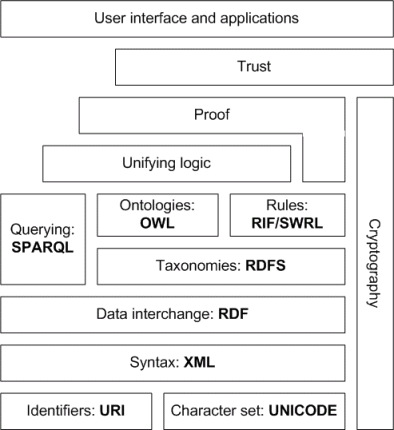
\includegraphics[scale=0.5]{Semantic-web-stack.png}
\caption{Semantic-web-stack}
\label{Semantic-web-stack}
\end{figure}

\subsection{Current state of standardization}

Well-established standards:

\begin{compactitem}
\item Unicode
\item Uniform Resource Identifier
\item XML
\item RDF
\item RDFS
\item SPARQL
\item Web Ontology Language (OWL)
\item Rule Interchange Format (RIF)
\end{compactitem}

Not yet fully realized:

\begin{compactitem}
\item Unifying Logic and Proof layers
\end{compactitem}

The intent is to enhance the usability and usefulness of the Web and its interconnected resources through:

\begin{compactitem}
\item Servers which expose existing data systems using the RDF and SPARQL standards. Many converters to RDF exist from different applications. Relational databases are an important source. The semantic web server attaches to the existing system without affecting its operation.
\item Documents "marked up" with semantic information (an extension of the HTML <meta> tags used in today's Web pages to supply information for Web search engines using web crawlers). This could be machine-understandable information about the human-understandable content of the document (such as the creator, title, description, etc.) or it could be purely metadata representing a set of facts (such as resources and services elsewhere on the site). Note that anything that can be identified with a Uniform Resource Identifier (URI) can be described, so the semantic web can reason about animals, people, places, ideas, etc. Semantic markup is often generated automatically, rather than manually.
\item Common metadata vocabularies (ontologies) and maps between vocabularies that allow document creators to know how to mark up their documents so that agents can use the information in the supplied metadata (so that Author in the sense of 'the Author of the page' won't be confused with Author in the sense of a book that is the subject of a book review)
\item Automated agents to perform tasks for users of the semantic web using this data
\item Web-based services (often with agents of their own) to supply information specifically to agents, for example, a Trust service that an agent could ask if some online store has a history of poor service or spamming
\end{compactitem}




\section{Skeptional reactions}


\subsection{Practical feasibility}

Critics (e.g. Which Semantic Web) question the basic feasibility of a complete or even partial fulfillment of the semantic web. Cory Doctorow's critique ("metacrap") is from the perspective of human behavior and personal preferences. For example, people may include spurious metadata into Web pages in an attempt to mislead Semantic Web engines that naively assume the metadata's veracity. This phenomenon was well-known with metatags that fooled the AltaVista ranking algorithm into elevating the ranking of certain Web pages: the Google indexing engine specifically looks for such attempts at manipulation. Peter Gärdenfors and Timo Honkela point out that logic-based semantic web technologies cover only a fraction of the relevant phenomena related to semantics.

Core, specialized communities and organizations for intra-company projects tended to practically adopt semantic web technologies greater than peripheral and less-specialized communities.[29] The practical constraints toward adoption have appeared less challenging where domain and scope is more limited than that of the general public and the World-Wide Web.[29]


\subsection{Censorship and privacy}

Enthusiasm about the semantic web could be tempered by concerns regarding censorship and privacy. For instance, text-analyzing techniques can now be easily bypassed by using other words, metaphors for instance, or by using images in place of words. An advanced implementation of the semantic web would make it much easier for governments to control the viewing and creation of online information, as this information would be much easier for an automated content-blocking machine to understand. In addition, the issue has also been raised that, with the use of FOAF files and geo location meta-data, there would be very little anonymity associated with the authorship of articles on things such as a personal blog. Some of these concerns were addressed in the "Policy Aware Web" project[30] and is an active research and development topic.

\subsection{Doubling output formats}

Another criticism of the semantic web is that it would be much more time-consuming to create and publish content because there would need to be two formats for one piece of data: one for human viewing and one for machines. However, many web applications in development are addressing this issue by creating a machine-readable format upon the publishing of data or the request of a machine for such data. The development of microformats has been one reaction to this kind of criticism. Another argument in defense of the feasibility of semantic web is the likely falling price of human intelligence tasks in digital labor markets, such as the Amazon Mechanical Turk.

Specifications such as eRDF and RDFa allow arbitrary RDF data to be embedded in HTML pages. The GRDDL (Gleaning Resource Descriptions from Dialects of Language) mechanism allows existing material (including microformats) to be automatically interpreted as RDF, so publishers only need to use a single format, such as HTML.


\section{Projects}

This section lists some of the many projects and tools that exist to create Semantic Web solutions.


\subsection{DBpedia}

DBPedia is an effort to publish structured data extracted from Wikipedia: the data is published in RDF and made available on the Web for use under the GNU Free Documentation License, thus allowing Semantic Web agents to provide inferencing and advanced querying over the Wikipedia-derived dataset and facilitating interlinking, re-use and extension in other data-sources.



\subsection{FOAF}

A popular vocabulary on the semantic web is Friend of a Friend (or FOAF), which uses RDF to describe the relationships people have to other people and the "things" around them. FOAF permits intelligent agents to make sense of the thousands of connections people have with each other, their jobs and the items important to their lives; connections that may or may not be enumerated in searches using traditional web search engines. Because the connections are so vast in number, human interpretation of the information may not be the best way of analyzing them.

FOAF is an example of how the Semantic Web attempts to make use of the relationships within a social context.

\subsection{SIOC}

The Semantically-Interlinked Online Communities project (SIOC, pronounced "shock") provides a vocabulary of terms and relationships that model web data spaces. Examples of such data spaces include, among others: discussion forums, blogs, blogrolls / feed subscriptions, mailing lists, shared bookmarks and image galleries.


\subsection{GoPubMed}

GoPubMed is a knowledge-based search engine for biomedical texts. The Gene Ontology (GO) and Medical Subject Headings (MeSH) serve as "Table of contents" in order to structure the millions of articles of the MEDLINE database. The search engine allows its users to find relevant search results significantly faster than Pubmed.


\subsection{NextBio}

A database consolidating high-throughput life sciences experimental data tagged and connected via biomedical ontologies. Nextbio is accessible via a search engine interface. Researchers can contribute their findings for incorporation to the database. The database currently supports gene expression or protein expression data and sequence centric data and is steadily expanding to support other biological data types.













\chapter{Delivery}

HTML documents can be delivered by the same means as any other computer file. However, they are most often delivered either by HTTP from a web server or by email.

\begin{compactitem}
\item HTTP

The World Wide Web is composed primarily of HTML documents transmitted from web servers to web browsers using the Hypertext Transfer Protocol (HTTP). However, HTTP is used to serve images, sound, and other content, in addition to HTML. To allow the web browser to know how to handle each document it receives, other information is transmitted along with the document. This meta data usually includes the MIME type (e.g. text/html or application/xhtml+xml) and the character encoding (see Character encoding in HTML).

In modern browsers, the MIME type that is sent with the HTML document may affect how the document is initially interpreted. A document sent with the XHTML MIME type is expected to be well-formed XML; syntax errors may cause the browser to fail to render it. The same document sent with the HTML MIME type might be displayed successfully, since some browsers are more lenient with HTML.

The W3C recommendations state that XHTML 1.0 documents that follow guidelines set forth in the recommendation's Appendix C may be labeled with either MIME Type. XHTML 1.1 also states that XHTML 1.1 documents should[59] be labeled with either MIME type.

万维网主要由从服务器通过HTTP协议向浏览器发送的HTML文档组成。但是,HTTP也可以被用于传输HTML之外的数据,例如图像、声音和其他内容。为使浏览器了解如何处理接收到的文档,在传输文档时必须同时传递文件类型。这种元数据包含MIME类型(对于HTML 4.01或更早版本是text/html,而对于XHTML 1.0或之后的版本是application/xhtml+xml),以及字符编码。

在现在的浏览器中,和HTML文档一起发送的MIME类型影响文档的解读方式。和XHTML MIME类型一起发送的文档被认为是良构的XML,而语法错误会导致浏览器无法呈现文档。完全相同的文档如果和HTML MIME类型一起发送,则可能被正常显示,因为浏览器对HTML的语法检查更加松懈些。

\item HTML e-mail

Most graphical email clients allow the use of a subset of HTML (often ill-defined) to provide formatting and semantic markup not available with plain text. This may include typographic information like coloured headings, emphasized and quoted text, inline images and diagrams. Many such clients include both a GUI editor for composing HTML e-mail messages and a rendering engine for displaying them. Use of HTML in e-mail is controversial because of compatibility issues, because it can help disguise phishing attacks, because of accessibility issues for blind or visually impaired people, because it can confuse spam filters and because the message size is larger than plain text.

一些图形模式下的电子邮件客户端支持HTML格式的邮件。很多支持一个图形模式下的HTML邮件编辑器,以及一个HTML邮件阅览器。因为一些问题,HTML邮件的使用有争议。HTML邮件的主要优点是可以使用呈现性元素来加强邮件的视觉效果,但是缺陷也很多,例如:

\begin{compactitem}
\item 收件人未必有一个可以浏览HTML邮件的客户端
\item 邮件大小增加。一些邮件客户端随HTML邮件发送一个纯文字版更加重了这个问题
\item 过度使用格式化
\item 潜在安全问题,例如伪造银行电子邮件用于网络钓鱼
\item 在一些有缺陷的电子邮件程序显示HTML邮件时可能执行恶意代码
\end{compactitem}

因为这些原因,很多新闻组和邮件列表要么截断信件的HTML部分,要么只接受纯文本版本部分的邮件,要么拒绝接收HTML邮件。

\item Naming conventions

The most common filename extension for files containing HTML is .html. A common abbreviation of this is .htm, which originated because some early operating systems and file systems, such as DOS and the limitations imposed by FAT data structure, limited file extensions to three letters.

\item HTML Application

An HTML Application (HTA; file extension ".hta") is a Microsoft Windows application that uses HTML and Dynamic HTML in a browser to provide the application's graphical interface. A regular HTML file is confined to the security model of the web browser's security, communicating only to web servers and manipulating only webpage objects and site cookies. An HTA runs as a fully trusted application and therefore has more privileges, like creation/editing/removal of files and Windows Registry entries. Because they operate outside the browser's security model, HTAs cannot be executed via HTTP, but must be downloaded (just like an EXE file) and executed from local file system .

\end{compactitem}





\chapter{Current variations}

Since its inception, HTML and its associated protocols gained acceptance relatively quickly. However, no clear standards existed in the early years of the language. Though its creators originally conceived of HTML as a semantic language devoid of presentation details, practical uses pushed many presentational elements and attributes into the language, driven largely by the various browser vendors. The latest standards surrounding HTML reflect efforts to overcome the sometimes chaotic development of the language[64] and to create a rational foundation for building both meaningful and well-presented documents. To return HTML to its role as a semantic language, the W3C has developed style languages such as CSS and XSL to shoulder the burden of presentation. In conjunction, the HTML specification has slowly reined in the presentational elements.


There are two axes differentiating various variations of HTML as currently specified: SGML-based HTML versus XML-based HTML (referred to as XHTML) on one axis, and strict versus transitional (loose) versus frameset on the other axis.


\section{SGML-based versus XML-based HTML}


One difference in the latest HTML specifications lies in the distinction between the SGML-based specification and the XML-based specification. The XML-based specification is usually called XHTML to distinguish it clearly from the more traditional definition. However, the root element name continues to be 'html' even in the XHTML-specified HTML. The W3C intended XHTML 1.0 to be identical to HTML 4.01 except where limitations of XML over the more complex SGML require workarounds. Because XHTML and HTML are closely related, they are sometimes documented in parallel. In such circumstances, some authors conflate the two names as (X)HTML or X(HTML).

Like HTML 4.01, XHTML 1.0 has three sub-specifications: strict, transitional and frameset.

Aside from the different opening declarations for a document, the differences between an HTML 4.01 and XHTML 1.0 document—in each of the corresponding DTDs—are largely syntactic. The underlying syntax of HTML allows many shortcuts that XHTML does not, such as elements with optional opening or closing tags, and even EMPTY elements which must not have an end tag. By contrast, XHTML requires all elements to have an opening tag and a closing tag. XHTML, however, also introduces a new shortcut: an XHTML tag may be opened and closed within the same tag, by including a slash before the end of the tag like this: <br/>. The introduction of this shorthand, which is not used in the SGML declaration for HTML 4.01, may confuse earlier software unfamiliar with this new convention. A fix for this is to include a space before closing the tag, as such: <br />.

To understand the subtle differences between HTML and XHTML, consider the transformation of a valid and well-formed XHTML 1.0 document that adheres to Appendix C (see below) into a valid HTML 4.01 document. To make this translation requires the following steps:

\begin{compactenum}
\item The language for an element should be specified with a lang attribute rather than the XHTML xml:lang attribute. XHTML uses XML's built in language-defining functionality attribute.
\item Remove the XML namespace (xmlns=URI). HTML has no facilities for namespaces.
\item Change the document type declaration from XHTML 1.0 to HTML 4.01. (see DTD section for further explanation).
\item If present, remove the XML declaration. (Typically this is: <?xml version="1.0" encoding="utf-8"?>).
\item Ensure that the document's MIME type is set to text/html. For both HTML and XHTML, this comes from the HTTP Content-Type header sent by the server.
\item Change the XML empty-element syntax to an HTML style empty element (<br/> to <br>).

\end{compactenum}
Those are the main changes necessary to translate a document from XHTML 1.0 to HTML 4.01. To translate from HTML to XHTML would also require the addition of any omitted opening or closing tags. Whether coding in HTML or XHTML it may just be best to always include the optional tags within an HTML document rather than remembering which tags can be omitted.

A well-formed XHTML document adheres to all the syntax requirements of XML. A valid document adheres to the content specification for XHTML, which describes the document structure.

The W3C recommends several conventions to ensure an easy migration between HTML and XHTML (see HTML Compatibility Guidelines). The following steps can be applied to XHTML 1.0 documents only:

\begin{compactitem}
\item Include both xml:lang and lang attributes on any elements assigning language.
\item Use the empty-element syntax only for elements specified as empty in HTML.
\item Include an extra space in empty-element tags: for example <br /> instead of <br/>.
\item Include explicit close tags for elements that permit content but are left empty (for example, <div></div>, not <div />).
\item Omit the XML declaration.
\end{compactitem}

By carefully following the W3C's compatibility guidelines, a user agent should be able to interpret the document equally as HTML or XHTML. For documents that are XHTML 1.0 and have been made compatible in this way, the W3C permits them to be served either as HTML (with a text/html MIME type), or as XHTML (with an application/xhtml+xml or application/xml MIME type). When delivered as XHTML, browsers should use an XML parser, which adheres strictly to the XML specifications for parsing the document's contents.



\section{Transitional versus strict}

HTML 4 defined three different versions of the language: Strict, Transitional (once called Loose) and Frameset. The Strict version is intended for new documents and is considered best practice, while the Transitional and Frameset versions were developed to make it easier to transition documents that conformed to older HTML specification or didn't conform to any specification to a version of HTML 4. The Transitional and Frameset versions allow for presentational markup, which is omitted in the Strict version. Instead, cascading style sheets are encouraged to improve the presentation of HTML documents. Because XHTML 1 only defines an XML syntax for the language defined by HTML 4, the same differences apply to XHTML 1 as well.

The Transitional version allows the following parts of the vocabulary, which are not included in the Strict version:

\begin{compactitem}

\item A looser content model

	\begin{compactitem}
	\item Inline elements and plain text are allowed directly in: body, blockquote, form, noscript and noframes
	\end{compactitem}

\item Presentation related elements
	
	\begin{compactitem}
	\item underline (u)(Deprecated. can confuse a visitor with a hyperlink.)
	\item strike-through (s)
	\item center (Deprecated. use CSS instead.)
	\item font (Deprecated. use CSS instead.)
	\item basefont (Deprecated. use CSS instead.)
	\end{compactitem}
	
\item Presentation related attributes
	\begin{compactitem}
	\item background (Deprecated. use CSS instead.) and bgcolor (Deprecated. use CSS instead.)  attributes for body (required element according to the W3C.) element.
	\item align (Deprecated. use CSS instead.) attribute on div, form, paragraph (p) and heading (h1...h6) elements
	\item align (Deprecated. use CSS instead.), noshade (Deprecated. use CSS instead.), size (Deprecated. use CSS instead.) and width (Deprecated. use CSS instead.) attributes on hr element
	\item align (Deprecated. use CSS instead.), border, vspace and hspace attributes on img and object (caution: the object element is only supported in Internet Explorer (from the major browsers)) elements
	\item align (Deprecated. use CSS instead.) attribute on legend and caption elements
	\item align (Deprecated. use CSS instead.) and bgcolor (Deprecated. use CSS instead.) on table element
	\item nowrap (Obsolete), bgcolor (Deprecated. use CSS instead.), width, height on td and th elements
	\item bgcolor (Deprecated. use CSS instead.) attribute on tr element
	\item clear (Obsolete) attribute on br element
	\item compact attribute on dl, dir and menu elements
	\item type (Deprecated. use CSS instead.), compact (Deprecated. use CSS instead.) and start (Deprecated. use CSS instead.) attributes on ol and ul elements
	\item type and value attributes on li element
	\item width attribute on pre element
	\end{compactitem}
	
\item Additional elements in Transitional specification
	
	\begin{compactitem}
	\item menu (Deprecated. use CSS instead.) list (no substitute, though unordered list is recommended)
	\item dir (Deprecated. use CSS instead.) list (no substitute, though unordered list is recommended)
	\item isindex (Deprecated.) (element requires server-side support and is typically added to documents server-side, form and input elements can be used as a substitute)
	\item applet (Deprecated. use the object element instead.)
	\end{compactitem}

\item The language (Obsolete) attribute on script element (redundant with the type attribute).
\item Frame related entities
	\begin{compactitem}
	\item iframe
	\item noframes
	\item target (Deprecated in the map, link and form elements.) attribute on a, client-side image-map (map), link, form and base elements
	\end{compactitem}
	
\end{compactitem}

The Frameset version includes everything in the Transitional version, as well as the frameset element (used instead of body) and the frame element.



\section{Frameset versus transitional}

In addition to the above transitional differences, the frameset specifications (whether XHTML 1.0 or HTML 4.01) specifies a different content model, with frameset replacing body, that contains either frame elements, or optionally noframes with a body.



\section{Summary of specification versions}

As this list demonstrates, the loose versions of the specification are maintained for legacy support. However, contrary to popular misconceptions, the move to XHTML does not imply a removal of this legacy support. Rather the X in XML stands for extensible and the W3C is modularizing the entire specification and opening it up to independent extensions. The primary achievement in the move from XHTML 1.0 to XHTML 1.1 is the modularization of the entire specification. The strict version of HTML is deployed in XHTML 1.1 through a set of modular extensions to the base XHTML 1.1 specification. Likewise, someone looking for the loose (transitional) or frameset specifications will find similar extended XHTML 1.1 support (much of it is contained in the legacy or frame modules). The modularization also allows for separate features to develop on their own timetable. So for example, XHTML 1.1 will allow quicker migration to emerging XML standards such as MathML (a presentational and semantic math language based on XML) and XForms—a new highly advanced web-form technology to replace the existing HTML forms.

In summary, the HTML 4 specification primarily reined in all the various HTML implementations into a single clearly written specification based on SGML. XHTML 1.0, ported this specification, as is, to the new XML defined specification. Next, XHTML 1.1 takes advantage of the extensible nature of XML and modularizes the whole specification. XHTML 2.0 was intended to be the first step in adding new features to the specification in a standards-body-based approach.


\section{WhatWG HTML versus HTML5}


The WhatWG considers their work as living standard HTML for what constitutes the state of the art in major browser implementations by Apple (Safari), Google (Chrome), Mozilla (Firefox), Opera (Opera), and others. HTML5 is specified by the HTML Working Group of the W3C following the W3C process. As of 2013 both specifications are similar and mostly derived from each other, i.e., the work on HTML5 started with an older WhatWG draft, and later the WhatWG living standard was based on HTML5 drafts in 2011.









\chapter{Hypertext features not in HTML}

HTML lacks some of the features found in earlier hypertext systems, such as source tracking, fat links and others. Even some hypertext features that were in early versions of HTML have been ignored by most popular web browsers until recently, such as the link element and in-browser Web page editing.

Sometimes Web services or browser manufacturers remedy these shortcomings. For instance, wikis and content management systems allow surfers to edit the Web pages they visit.

HTML是一个相对比较弱的超文本实现。早期超文本系统具有具有类型的链接、跨越包含和来源跟踪这样的属性。另一个现在缺乏支持的特性是粗链路。

直到不久之前,一些早期HTML版本中的超文本特性一直被大多数浏览器忽略,例如link元素和可编辑的网页。

有时网络服务或者浏览器厂商也认识到这些特性。例如,现在的wiki和nuke社会网络软件允许浏览者编辑访问的网页。

\chapter{HTML editor}

An HTML editor is a computer program for creating web pages. Although the HTML markup of a web page can be written with any text editor, specialized HTML editors can offer convenience and added functionality. For example, many HTML editors work not only with HTML, but also with related technologies such as CSS, XML and JavaScript or ECMAScript. In some cases they also manage communication with remote web servers via FTP and WebDAV, and version management systems such as CVS or Subversion.

There are various forms of HTML editors: text, object and WYSIWYG (what you see is what you get) editors.


\section{Text editors}

Text (source) editors intended for use with HTML usually provide syntax highlighting. Templates, toolbars and keyboard shortcuts may quickly insert common HTML elements and structures. Wizards, tooltip prompts and autocompletion may help with common tasks.

Text HTML editors commonly include either built-in functions or integration with external tools for such tasks as source and version control, link-checking, code checking and validation, code cleanup and formatting, spell-checking, uploading by FTP or WebDAV, and structuring as a project.

Text editors require user understanding of HTML and any other web technologies the designer wishes to use like CSS, JavaScript and server-side scripting languages. They were also referred to A Simple HTML Editor (ASHE).

Some regular text editors such as Windows Notepad can save as HTML files simply by using extensions such as .html .htm .css etc.


\section{Object editors}

Some editors allow alternate editing of the source text of objects in more visually organized modes than simple color highlighting, but in modes not considered WYSIWYG. Some WYSIWYG editors include the option of using palette windows that enable editing the text-based parameters of selected objects. These palettes allow either editing parameters in fields for each individual parameter, or text windows to edit the full group of source text for the selected object. They may include widgets to present and select options when editing parameters. Adobe GoLive provides an outline editor to expand and collapse HTML objects and properties, edit parameters, and view graphics attached to the expanded objects.




\section{WYSIWYG editors}

There are some WYSIWYG (What You See Is What You Get) editors, in which the user lays out everything as it is to appear in the HTML document using a graphical user interface (GUI), often similar to word processors. The editor renders the document rather than show the code, so authors do not require extensive knowledge of HTML.



The WYSIWYG editing model has been criticized, primarily because of the low quality of the generated code; there are voices advocating a change to the WYSIWYM model (What You See Is What You Mean).

WYSIWYG HTML editors provide an editing interface which resembles how the page will be displayed in a web browser. These editors may be stand-alone programs, such as Adobe Dreamweaver or Microsoft Frontpage, or come in the form of browser extensions and allow editing directly within the web browser. Because using a WYSIWYG editor may not require any HTML knowledge, they are often easier for an average computer user to get started with.

WYSIWYG editors remain a controversial topic because of their perceived flaws such as:

\begin{compactitem}
\item Relying mainly on layout as opposed to meaning, often using markup that does not convey the intended meaning but simply copies the layout.
\item Often producing extremely verbose and redundant code that fails to make use of the cascading nature of HTML and CSS.
\item Often producing ungrammatical markup often called tag soup or semantically incorrect markup (such as <em> for italics).
\item As a great deal of the information in HTML documents is not in the layout, the model has been criticized for its "what you see is all you get"-nature
\end{compactitem}

The WYSIWYG view is achieved by embedding a layout engine based upon that used in a web browser. The layout engine will have been considerably enhanced by the editor's developers to allow for typing, pasting, deleting and manipulation of the content. The goal is that, at all times during editing, the rendered result should represent what will be seen later in a typical web browser.

\section{WYSIWYM editors}

WYSIWYM (what you see is what you mean) is an alternative paradigm to the WYSIWYG editors above. Instead of focusing on the format or presentation of the document, it preserves the intended meaning of each element. For example, page headers, sections, paragraphs, etc. are labeled as such in the editing program, and displayed appropriately in the browser.

\section{Online editors}

There are many online WYSIWYG HTML editors, some of them are:

\begin{compactitem}
\item CLEditor
\item CKEditor
\item OpenBEXI
\item SnapEditor
\item TinyMCE
\item WYMeditor
\item YUI Rich Text Editor
\end{compactitem}

\section{Difficulties in achieving WYSIWYG}


A given HTML document will have an inconsistent appearance on various platforms and computers for several reasons:

\begin{compactitem}
\item Different browsers and applications will render the same markup differently.

The same page may display slightly differently in Internet Explorer and Firefox on a high-resolution screen, but it will look very different in the perfectly valid text-only Lynx browser. It needs to be rendered differently again on a PDA, an internet-enabled television and on a mobile phone. Usability in a speech or braille browser, or via a screen-reader working with a conventional browser, will place demands on entirely different aspects of the underlying HTML. Printing the page, via different browsers and different printers onto various paper sizes, around the world, places other demands. With the correct use of modern HTML and CSS there is no longer any need to provide 'Printable page' links and then have to maintain two versions of the whole site. Nor is there any excuse for pages not fitting the user's preferred paper size and orientation, or wasting ink printing solid background colours unnecessarily, or wasting paper reproducing navigation panels that will be entirely useless once printed out.

\item Browsers and computer graphics systems have a range of user settings.

Resolution, font size, colour, contrast etc can all be adjusted at the user's discretion, and many modern browsers allow even more user control over page appearance. All an author can do is suggest an appearance.

\item Web browsers, like all computer software, have bugs

They may not conform to current standards. It is hopeless to try to design Web pages around all of the common browsers' current bugs: each time a new version of each browser comes out, a significant proportion of the World Wide Web would need re-coding to suit the new bugs and the new fixes. It is generally considered much wiser to design to standards, staying away from 'bleeding edge' features until they settle down, and then wait for the browser developers to catch up to your pages, rather than the other way round. For instance, no one can argue that CSS is still 'cutting edge' as there is now widespread support available in common browsers for all the major features, even if many WYSIWYG and other editors have not yet entirely caught up.

\item A single visual style can represent multiple semantic meanings

Semantic meaning, derived from the underlying structure of the HTML document, is important for search engines and also for various accessibility tools. On paper we can tell from context and experience whether bold text represents a title, or emphasis, or something else. But it is very difficult to convey this distinction in a WYSIWYG editor. Simply making a piece of text bold in a WYSIWYG editor is not sufficient to tell the editor *why* the text is bold - what the boldness represents semantically.

\end{compactitem}

What you see may be what most visitors get, but it is not guaranteed to be what everyone gets.



\chapter{HTML Parser}

Parsing HTML is a automated task, performed by (so called) HTML parsers. They have two main purposes:

\begin{compactitem}
\item HTML traversal

offer a interface for programmers to easily access and modify of the "HTML string code". Canonical example: DOM parsers.
\item HTML clean

To fix invalid HTML and to improve the layout and indent style of the resulting markup. Canonical example: HTML Tidy.
\end{compactitem}










































\part{HTML Elements}

An HTML element is an individual component of an HTML document or "web page", once this has been parsed into the Document Object Model. HTML is composed of a tree of HTML elements and other nodes, such as text nodes. Each element can have HTML attributes specified. Elements can also have content, including other elements and text. HTML elements represent semantics, or meaning. For example, the title element represents the title of the document.

HTML 允许开发者格式化文本,添加图片,创建链接、输入表单、框架和表格等等,并可将之存为文本文件,浏览器即可读取和显示。

HTML 元素指的是从开始标签(start tag)到结束标签(end tag)的所有代码\footnote{开始标签常被称为开放标签(opening tag),结束标签常称为闭合标签(closing tag)。}。元素(elements)用于结构化HTML文档,并告知浏览器如何呈现网页。一般来说,元素由首标签(start tag)、内容(content)和尾标签(end tag)构成,因此HTML 的关键是标签,其作用是指示将出现的内容。




\begin{compactitem}
\item HTML 标签是由尖括号包围的关键词,比如 <html>
\item HTML 标签通常是成对出现的,比如 <b> 和 </b>
\item 标签对中的第一个标签是开始标签,第二个标签是结束标签
\item 开始和结束标签也被称为开放标签和闭合标签
\end{compactitem}




In the HTML syntax, most elements are written with a start tag and an end tag, with the content in between. An HTML tag is composed of the name of the element, surrounded by angle brackets. An end tag also has a slash after the opening angle bracket, to distinguish it from the start tag. For example, a paragraph, which is represented by the p element, would be written as

\begin{lstlisting}[language=HTML]
<p>In the HTML syntax, most elements are written ...</p>
\end{lstlisting}


However, not all of these elements require the end tag, or even the start tag, to be present. Some elements, the so-called void elements, do not have an end tag. A typical example is the br element, which represents a significant line break, such as in a poem or an address. A void element's behaviour is predefined, and it can not contain any content or other elements. For example, the address of the dentist in Finding Nemo would be written as


\begin{lstlisting}[language=HTML]
<p>P. Sherman<br>42 Wallaby Way<br>Sydney</p>
\end{lstlisting}

首标签和尾标签总是必须的吗?

常言道,凡事均有例外。在HTML中,也有例外的情况,即有些元素没有尾标签。这些没有尾标签的元素被称作空元素(empty element),它们与具体文本内容无关,比如像下面这个换行标签:<br />。

大多数浏览器不介意标签是大写还是小写,或者混合大小写。所以<HTML>、<html>或<HtMl>在浏览器上的显示效果都一样。但是,正确的写法是采用小写字母来书写标签。所以,要养成用小写字母书写标签的习惯\footnote{HTML 标签对大小写不敏感:<P> 等同于 <p>,但万维网联盟(W3C)在 HTML 4 中推荐使用小写,而在未来 (X)HTML 版本中强制使用小写。}。

创建HTML文档的过程,也就是在HTML文档里书写标签。一个网站可能包含多个HTML文档。上网的过程,其实就是打开不同HTML文档的过程。

浏览器解析HTML就跟我们读书一样,也是从上往下,从左到右进行的。所以,HTML文档的开始和结束便对应于网页的头和尾。

\begin{compactitem}
\item HTML 文档描述网页
\item HTML 文档包含 HTML 标签和纯文本
\item HTML 文档也被称为网页
\end{compactitem}

When using an XHTML DTD, it is required to open and close the element with a single tag. To specify that it is a void element, a "/" is included at the end of the tag (not to be confused with the "/" at the beginning of a closing tag).

\begin{lstlisting}[language=HTML]
<p>P. Sherman<br/>42 Wallaby Way<br/>Sydney</p>
\end{lstlisting}

标签(tag)指示元素的起始与结束,并且所有标签都具有相同的格式:以小于号“<”开头,以大于号“>”结尾。

一般说来,有两种标签——首标签(start tag)(如<html>)和尾标签(end tag)(如</html>)。它们唯一的区别在于,尾标签多一条斜杠“/。用户通过把内容放在首标签和尾标签之间来对内容进行标记。

HTML主要就是各种各样的元素,所以,学习HTML,就是学习使用各种元素。

\begin{lstlisting}[language=HTML]
<!DOCTYPE html>
<html>
	<head>
		<title>My first HTML.</title>
	</head>
	<body>
	<h1>My first Heading</h1>
	<p>My first paragraph.</p>
	</body>
</html>
\end{lstlisting}

\begin{compactitem}
\item <html> 与 </html> 之间的文本描述网页
\item <head>与</head>之间的文本提供当前网页的信息
\item <title>与</title>之间的文本指定HTML文档的标题
\item <body> 与 </body> 之间的文本是可见的页面内容
\item <h1> 与 </h1> 之间的文本被显示为标题
\item <p> 与 </p> 之间的文本被显示为段落
\end{compactitem}

其中:

\begin{compactitem}
\item <html> 元素定义了整个 HTML 文档。
这个元素拥有一个开始标签 <html>,以及一个结束标签 </html>。
\item <body> 元素定义了 HTML 文档的主体。
这个元素拥有一个开始标签 <body>,以及一个结束标签 </body>。
\item <p> 元素定义了 HTML 文档中的一个段落。
这个元素拥有一个开始标签 <p>,以及一个结束标签 </p>。
\item 即使用户忘记了使用结束标签,大多数浏览器也会正确地显示 HTML\footnote{未来的 HTML 版本不允许省略结束标签。}。
\end{compactitem}

注意,网页标题(title)不是显示在网页里,而是显示在浏览器窗口的标题栏上的。网页里显示的所有内容都必须放在body元素里。

网页标题(title)尤其重要,因为搜索引擎(比如Google)要用它来索引网页,并显示在搜索结果里。

HTML attributes are specified inside the start tag. For example, the abbr element, which represents an abbreviation, expects a title attribute within its opening tag. This would be written as


\begin{lstlisting}[language=HTML]
	<abbr title="abbreviation">abbr.</abbr>
\end{lstlisting}


\chapter{Concepts}


\section{Document vs. DOM}

HTML documents are delivered as "documents". These are then parsed, which turns them into the Document Object Model (DOM) internal representation, within the web browser.

Presentation by the web browser, such as screen rendering or access by JavaScript, is then performed on this internal model, not the original document.

Early HTML documents, and to a lesser extent today, were largely invalid HTML and riddled with syntax errors. The parsing process was also required to "fix-up" these errors, as best it could. The resultant model was often not correct (i.e. it did not represent what a careless coder had originally intended), but it would at least be valid, according to the HTML standard. A valid model was produced, no matter how bad the "tag soup" supplied had been. Only in the rarest cases would the parser abandon parsing altogether.


\section{Elements vs. tags}

"Elements" and "tags" are terms that are widely confused. HTML documents contain tags, but do not contain the elements. The elements are only generated after the parsing step, from these tags.

As is generally understood, the position of an element is indicated as spanning from a start tag, possibly including some child content, and is terminated by an end tag. This is the case for many, but not all, elements within an HTML document.

As HTML is based on SGML, its parsing also depends on the use of a DTD, specifically an HTML DTD such as that for HTML 4.01. The DTD specifies which element types are possible (i.e. it defines the set of element types that go to make up HTML) and it also specifies the valid combinations in which they may appear in a document. It is part of general SGML behaviour that where only one valid structure is possible (per the DTD), it is not generally a requirement that the document explicitly states that structure. As a simple example, the <p> start tag indicating the start of a paragraph element should be closed by a </p> end tag, indicating the end of the element. Also the DTD states that paragraph elements cannot be nested. The HTML document fragment:


\begin{lstlisting}[language=HTML]
<p>Para 1 <p>Para 2 <p>Para 3
\end{lstlisting}

can thus be inferred to be equivalent to:

\begin{lstlisting}[language=HTML]
<p>Para 1 </p><p>Para 2 </p><p>Para 3
\end{lstlisting}

(If one paragraph element cannot contain another, any currently open paragraph must be closed before starting another.)

Because of this implied behaviour, based on the combination of the DTD and the individual document, it is not possible to infer elements from the document tags alone, but only by also using an SGML or HTML aware parser, with knowledge of the DTD.


\section{SGML vs. XML}

SGML is complex, which has limited its widespread adoption and understanding. XML was developed as a simpler alternative. XML is similar to SGML, and can also use the DTD mechanism to specify the elements supported and their permitted combinations as document structure. XML parsing is however simpler. The relation from tags to elements is always simply that of parsing the actual tags included in the document, without the implied closures that are part of SGML.

Where HTML can be formed as XML, either through XHTML or through HTML5 as XML, the parsing from document tags to DOM elements is simplified, but still follows the same basic process. Once the DOM of elements is obtained, behaviour beyond that point (i.e. screen rendering) is identical.


\section{Content vs. Presentation}

Since HTML 4, HTML has increasingly focussed on the separation of content from presentation.[7] This is often referred to as a separation of concerns. HTML is used to represent the structure or content of a document, its presentation remains the sole responsibility of CSS. A default style sheet is suggested as part of the CSS standard, giving a default rendering for HTML.


\section{\%block; vs. box}


Part of this CSS presentation behaviour is the notion of the "box model". This is applied to those elements that CSS considers to be "block" elements, set through the CSS display: block; statement.

HTML also has a similar concept, although different, and the two are very frequently confused. \%block; and \%inline; are groups within the HTML DTD that group elements as being either "block-level" or "inline".[9] This is used to define their nesting behaviour: block-level elements cannot be placed into an inline context.[note 7] This behaviour cannot be changed, it is fixed in the DTD. Block and inline elements have the appropriate and different CSS behaviours attached to them by default,[9] including the relevance of the box model for particular element types.

Note though that this CSS behaviour can, and frequently is, changed from the default. Lists with <ul><li> ... are \%block; elements and are presented as block elements by default. However, it is quite common to set these with CSS to display as an inline list.






\chapter{Overview}

\section{Syntax}


There are multiple kinds of HTML elements: void elements, raw text elements, and normal elements.


\begin{compactenum}
\item Void elements

Void elements only have a start tag, which contains any HTML attributes. They may not contain any children, such as text or other elements. Often they are place holders for elements which reference external files, such as the image (<img/>) element. The attributes included in the element will then point to the external file in question. Another example of a void element is the link element, for which the syntax is

\begin{lstlisting}[language=HTML]
<link rel="stylesheet" href="fancy.css" type="text/css">
\end{lstlisting}

This link element points the browser at a style sheet to use when presenting the HTML document to the user. Note that in the HTML syntax, attributes don't have to be quoted. When using the XML syntax (XHTML), on the other hand, all attributes must be quoted, and a trailing slash is required before the last angle bracket:


\begin{lstlisting}[language=HTML]
<link rel="stylesheet" href="fancy.css" type="text/css" />
\end{lstlisting}


\item Raw text elements

Raw text elements are constructed with:

\begin{compactitem}
\item a start tag (<tag>) marking the beginning of an element, which may incorporate any number of HTML attributes;
\item some amount of text content, but no elements (all tags, apart from the applicable end tag, will be interpreted as content);
\item an end tag, in which the element name is prefixed with a slash: </tag>. In some versions of HTML, the end tag is optional for some elements. The end tag is required in XHTML.
\end{compactitem}

\item Normal elements

Normal elements usually have both a start tag and an end tag, although for some elements the end tag, or both tags, can be omitted. It is constructed in a similar way:

\begin{compactitem}
\item a start tag (<tag>) marking the beginning of an element, which may incorporate any number of HTML attributes;
\item some amount of content, including text and other elements;
\item an end tag, in which the element name is prefixed with a slash: </tag>.
\end{compactitem}

\end{compactenum}


\begin{figure}
\centering
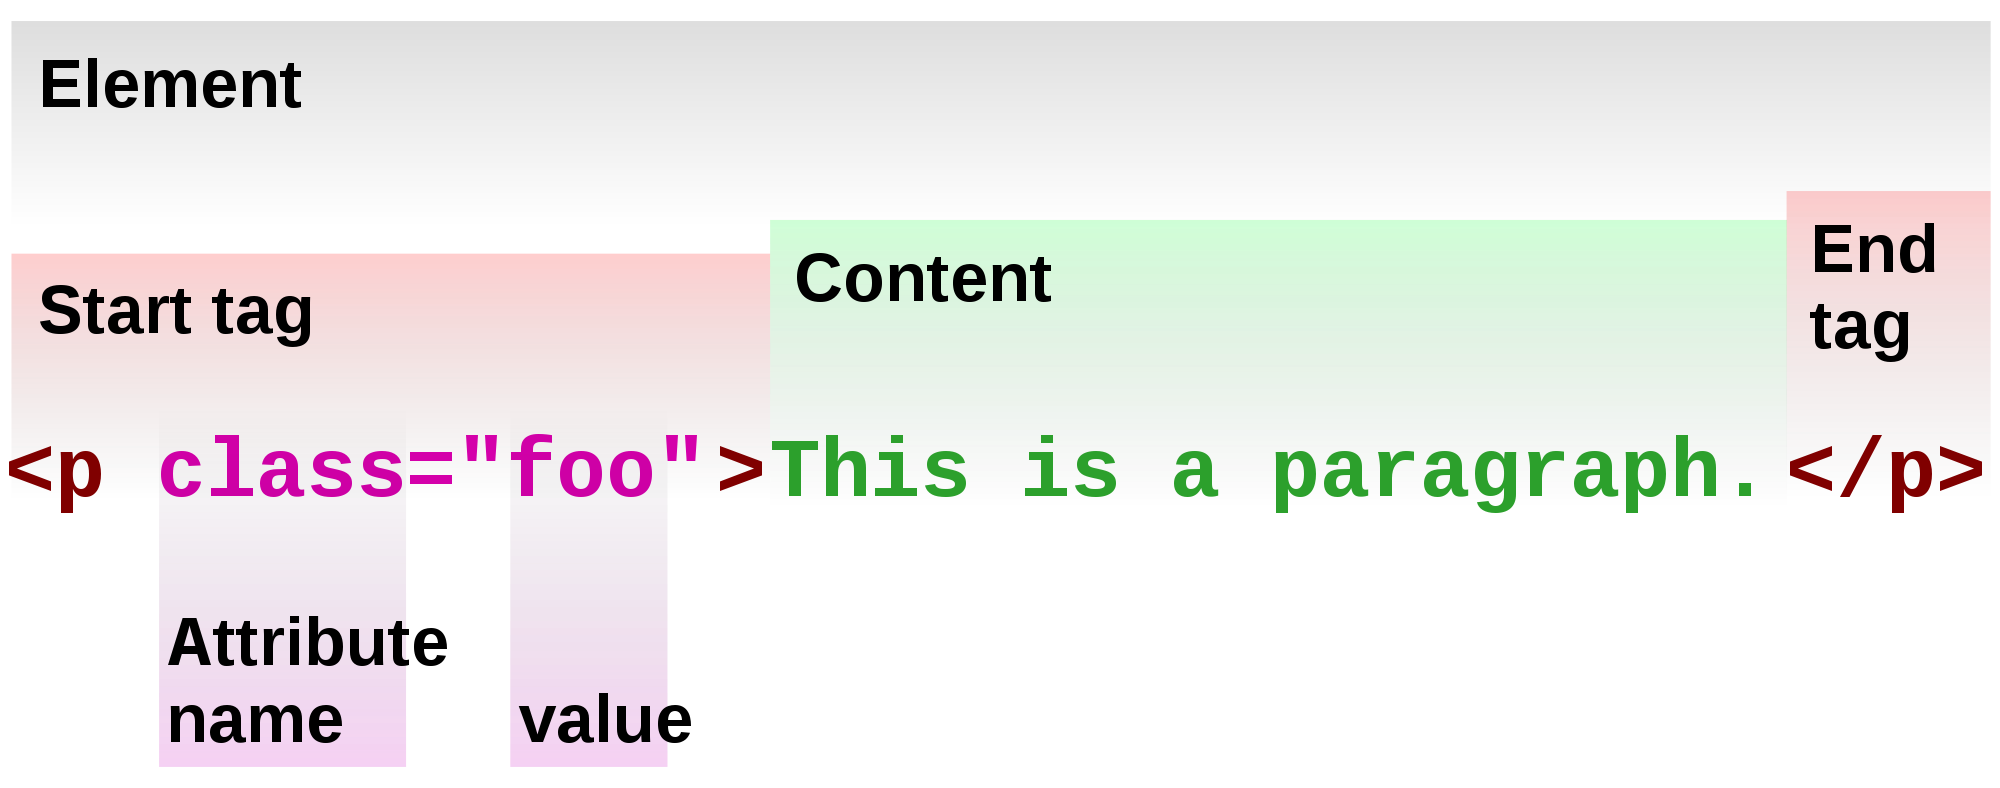
\includegraphics[scale=0.15]{2000px-HTML_element_structure.png}
\caption{Parts of an HTML container element}
\label{HTML_element_structure}
\end{figure}

Parts of an HTML container element:

\begin{compactitem}
\item Start tag: <p ... >
	\begin{compactitem}
	\item Attribute:
		\begin{compactitem}
		\item name: class
		\item value: foo
		\end{compactitem}
	\end{compactitem}
\item Content: This is a paragraph.
\item End tag: </p>
\end{compactitem}



HTML attributes define desired behaviour or indicate additional element properties. Most attributes require a value. In HTML, the value can be left unquoted if it doesn't include spaces (name=value), or it can be quoted with single or double quotes (name='value' or name="value"). In XML, those quotes are required. Boolean attributes, on the other hand, don't require a value to be specified. An example is the checked for checkboxes:



\begin{lstlisting}[language=HTML]
<input type=checkbox checked>
\end{lstlisting}

In the XML syntax, though, the name should be repeated as the value:

\begin{lstlisting}[language=HTML]
<input type="checkbox" checked="checked" />
\end{lstlisting}


Informally, HTML elements are sometimes referred to as "tags" (an example of synecdoche), though many prefer the term tag strictly in reference to the markup delimiting the start and end of an element.

Element (and attribute) names may be written in any combination of upper or lower case in HTML, but must be in lower case in XHTML.[11] The canonical form was upper-case until HTML 4, and was used in HTML specifications, but in recent years, lower-case has become more common.


HTML 元素语法

\begin{compactitem}
\item HTML 元素以开始标签起始
\item HTML 元素以结束标签终止
\item 元素的内容是开始标签与结束标签之间的内容
\item 某些 HTML 元素具有空内容(empty content)
\item 空元素在开始标签中进行关闭(以开始标签的结束而结束)
\item 大多数 HTML 元素可拥有属性
\end{compactitem}

我们无法确定 HTML 被显示的确切效果。屏幕的大小,以及对窗口的调整都可能导致不同的结果。
对于 HTML,用户无法通过在 HTML 代码中添加额外的空格或换行来改变输出的效果。

当显示页面时,浏览器会移除源代码中多余的空格和空行。所有连续的空格或空行都会被算作一个空格。需要注意的是,HTML 代码中的所有连续的空行(换行)也被显示为一个空格。

\section{Elements standards}


HTML elements are defined in a series of freely available open standards issued since 1995, initially by the IETF and subsequently by the W3C.

Since the early 1990s, developers of user agents (e.g. web browsers) have often developed their own elements, some of which have been adopted in later standards. Other user agents may not recognize non-standard elements, and they may be ignored or displayed improperly.

In 1998, XML (a simplified form of SGML) introduced mechanisms to allow anyone to develop their own elements and incorporate them in XHTML documents, for use with XML-aware user agents.

Subsequently, HTML 4.01 was rewritten in an XML-compatible form, XHTML 1.0 (eXtensible HTML). The elements in each are identical, and in most cases valid XHTML 1.0 documents will be valid or nearly valid HTML 4.01 documents. This article mainly focuses on real HTML, unless noted otherwise; however, it remains applicable to XHTML. (See HTML for a discussion of the minor differences between the two).


\section{Elements status}


Since the first version of HTML, several elements have become outmoded, and are deprecated in later standards, or do not appear at all, in which case they are invalid (and will be found invalid, and perhaps not displayed, by validating user agents).

At present, the status of elements is complicated by the existence of three types of HTML 4.01 / XHTML 1.0 DTD:

\begin{compactitem}
\item Transitional, which contain deprecated elements, but which were intended to provide a transitional period during which authors could update their practices;
\item Frameset, which are versions of the Transitional DTDs which also allow authors to write frameset documents;
\item Strict, which is the up-to date (as at 1999) form of HTML.
\end{compactitem}

The first Standard (HTML 2.0) contained four deprecated elements, one of which was invalid in HTML 3.2. All four are invalid in HTML 4.01 Transitional, which also deprecated a further ten elements. All of these, plus two others, are invalid in HTML 4.01 Strict. While the frame elements are still current in the sense of being present in the Transitional and Frameset DTDs, there are no plans to preserve them in future standards, as their function has been largely replaced, and they are highly problematic for user accessibility.


(Strictly speaking, the most recent XHTML standard, XHTML 1.1 (2001), does not include frames at all; it is approximately equivalent to XHTML 1.0 Strict, but also includes the Ruby markup module.)

A common source of confusion is the loose use of deprecated to refer to both deprecated and invalid status, and to elements which are expected to be formally deprecated in future.

\section{Presentation and behaviour}





In keeping with the principle of separation of concerns, the function of HTML is primarily to add structural and semantic information to the raw text of a document. Presentation and behaviour are separate functions, which can be added as desired, ideally through links to external documents such as style sheets, graphics files, and scripts.

This allows the document to be presented by different user agents according to their purposes and abilities; for example, a user agent can select an appropriate style sheet to present a document by displaying on a monitor, printing on paper, or to determine speech characteristics in an aural user agent. The structural and semantic functions of the markup remain identical in each case.

Historically, user agents did not always support these features. In the 1990s, as a stop-gap, presentational elements were added to HTML, at the cost of creating problems for interoperability and user accessibility. This is now regarded as outmoded and has been superseded by style sheet-based design; most presentational elements are now deprecated.

External image files are incorporated with the img or object elements. (With XHTML, the SVG language can also be used to write graphics within the document, though linking to external SVG files is generally simpler.) Where an image is not purely decorative, HTML allows replacement content with similar semantic value to be provided for non-visual user agents.


An HTML document can also be extended through the use of scripts to provide additional behaviours beyond the abilities of HTML hyperlinks and forms.

The elements style and script, with related HTML attributes, provide reference points in HTML markup for links to style sheets and scripts. They can also contain instructions directly.

\begin{compactitem}
\item In the document head, script and style may either link to shared external documents, or contain embedded instructions. (The link element can also be used to link style sheets.)
\item The style attribute is valid in most document body elements for inclusion of inline style instructions.
\item Event-handling attributes, which provide links to scripts, are optional in most elements.
script can occur at any point in the document body.
\item For user agents which do not operate scripts, the noscript element provides alternative content where appropriate; however, it can only be used as a block-level element.
\end{compactitem}


\section{List of all HTML4.01/XHTML1.0 elements}

DTD:指示在哪种 XHTML 1.0 DTD 中允许该标签。S=Strict, T=Transitional, F=Frameset。



\begin{longtable}{|p{60pt}|p{320pt}|p{40pt}|}
\multicolumn{3}{r}{...}
\tabularnewline\hline
Tag				& Description		& DTD		
\endhead
\hline
Tag				& Description		& DTD	
\tabularnewline\hline
\endfirsthead
\multicolumn{3}{r}{...}
\endfoot
%\tabularnewline\hline
\endlastfoot
<!--...-->		&	Defines a comment			& STF	\\
\hline
<!DOCTYPE>	&	Defines the document type	& STF	\\
\hline
<a>			&	Defines a hyperlink			& STF	\\
\hline
<abbr>		&	Defines an abbreviation		& STF	\\
\hline
<acronym>	&	Not supported in HTML5. Defines an acronym	& STF	\\
\hline
<address>	&	Defines contact information for the author/owner of a document & STF\\
\hline
<applet>		&	Not supported in HTML5. Deprecated in HTML 4.01. Defines an embedded applet	& TF	\\
\hline
<area>		&	Defines an area inside an image-map & STF\\
\hline
<article>		&	Defines an article & STF\\
\hline
<aside>		&	Defines content aside from the page content & STF\\
\hline
<audio>		&	Defines sound content & STF\\
\hline
<b>			&	Defines bold text & STF\\
\hline
<base>		&	Specifies the base URL/target for all relative URLs in a document & STF\\
\hline
<basefont>	&	Not supported in HTML5. Deprecated in HTML 4.01. Specifies a default colour, size, and font for all text in a document & TF\\
\hline
<bdi>		&	Isolates a part of text that might be formatted in a different direction from other text outside it & STF\\
\hline
<bdo>		&	Overrides the current text direction & STF\\
\hline
<big>		&	Not supported in HTML5. Defines big text & STF\\
\hline
<blockquote>	&	Defines a section that is quoted from another source & STF\\
\hline
<body>		&	Defines the document's body & STF\\
\hline
<br>			&	Defines a single line break	& STF\\
\hline
<canvas>		&	Used to draw graphics, on the fly, via scripting (usually JavaScript) & STF\\
\hline
<caption>		&	Defines a table caption & STF\\
\hline
<center>		&	Not supported in HTML5. Deprecated in HTML 4.01. Defines centred text & TF\\
\hline
<cite>		&	Defines the title of a work & STF\\
\hline
<code>		&	Defines a piece of computer code & STF\\
\hline
<col>		&	Specifies column properties for each column within a <colgroup> element  & STF\\
\hline
<colgroup>	&	Specifies a group of one or more columns in a table for formatting	& STF\\
\hline
<command>	&	Defines a command button that a user can invoke	& STF\\
\hline
<datalist>	&	Specifies a list of pre-defined options for input controls & STF\\
\hline
<dd>		&	Defines a description of an item in a definition list & STF\\
\hline
<del>		&	Defines text that has been deleted from a document & STF\\
\hline
<details>		&	Defines additional details that the user can view or hide & STF\\
\hline
<dfn>		&	Defines a definition term & STF\\
\hline
<dialog>		&	Defines a dialog box or window & STF\\
\hline
<dir>		&	Not supported in HTML5. Deprecated in HTML 4.01. Defines a directory list & TF\\
\hline
<div>		&	Defines a section in a document	& STF\\
\hline
<dl>			&	Defines a definition list & STF\\
\hline
<dt>			&	Defines a term (an item) in a definition list & STF\\
\hline
<em>		&	Defines emphasized text & STF\\
\hline
<embed>		&	Defines a container for an external (non-HTML) application & STF\\
\hline
<fieldset>	&	Groups related elements in a form	& STF\\
\hline
<figcaption>	&	Defines a caption for a <figure> element & STF\\
\hline
<figure>		&	Specifies self-contained content & STF\\
\hline
<font>		&	Not supported in HTML5. Deprecated in HTML 4.01. Defines font, colour, and size for text & TF\\
\hline
<footer>		&	Defines a footer for a document or section & STF\\
\hline
<form>		&	Defines an HTML form for user input & STF\\
\hline
<frame>		&	Not supported in HTML5. Defines a window (a frame) in a frameset & F \\
\hline
<frameset>	&	Not supported in HTML5. Defines a set of frames & F\\
\hline
<h1> to <h6>	&	Defines HTML headings & STF\\
\hline
<head>		&	Defines information about the document & STF\\
\hline
<header>		&	Defines a header for a document or section & STF\\
\hline
<hgroup>		&	Groups heading (<h1> to <h6>) elements & STF\\
\hline
<hr>			&	Defines a thematic change in the content & STF\\
\hline
<html>		&	Defines the root of an HTML document & STF\\
\hline
<i>			&	Defines a part of text in an alternate voice or mood & STF\\
\hline
<iframe>		&	Defines an inline frame & TF\\
\hline
<img>		&	Defines an image & STF\\
\hline
<input>		&	Defines an input control & STF\\
\hline
<ins>		&	Defines a text that has been inserted into a document & STF\\
\hline
<kbd>		&	Defines keyboard input & STF\\
\hline
<keygen>		&	Defines a key-pair generator field (for forms) & STF\\
\hline
<label>		&	Defines a label for an <input> element & STF\\
\hline
<legend>		&	Defines a caption for a <fieldset>, < figure>, or <details> element & STF\\
\hline
<li>			&	Defines a list item & STF\\
\hline
<link>		&	Defines the relationship between a document and an external resource (most used to link to style sheets)	 & STF\\
\hline
<map>		&	Defines a client-side image-map & STF\\
\hline
<mark>		&	Defines marked/highlighted text & STF\\
\hline
<menu>		&	Defines a list/menu of commands &TF\\
\hline
<meta>		&	Defines metadata about an HTML document & STF\\
\hline
<meter>		&	Defines a scalar measurement within a known range (a gauge) & STF\\
\hline
<nav>		&	Defines navigation links & STF\\
\hline
<noframes>	&	Not supported in HTML5. Defines an alternate content for users that do not support frames & TF\\
\hline
<noscript>	&	Defines an alternate content for users that do not support client-side scripts & STF\\
\hline
<object>		&	Defines an embedded object & STF\\
\hline
<ol>			&	Defines an ordered list & STF\\
\hline
<optgroup>	&	Defines a group of related options in a drop-down list & STF\\
\hline
<option>		&	Defines an option in a drop-down list & STF\\
\hline
<output>		&	Defines the result of a calculation & STF\\
\hline
<p>			&	Defines a paragraph & STF\\
\hline
<param>		&	Defines a parameter for an object & STF\\
\hline
<pre>		&	Defines pre-formatted/space-preserving text & STF\\
\hline
<progress>	&	Represents the progress of a task & STF\\
\hline
<q>			&	Defines a short quotation & STF\\
\hline
<rp>			&	Defines what to show in browsers that do not support ruby annotations & STF\\
\hline
<rt>			&	Defines an explanation/pronunciation of characters (for East Asian typography) & STF\\
\hline
<ruby>		&	Defines a ruby annotation (for East Asian typography) & STF\\
\hline
<s>			&	Defines text that is no longer correct	& TF\\
\hline
<samp>		&	Defines sample output from a computer program & STF\\
\hline
<script>		&	Defines a client-side script & STF\\
\hline
<section>		&	Defines a section in a document & STF\\
\hline
<select>		&	Defines a drop-down list & STF\\
\hline
<small>		&	Defines smaller text & STF\\
\hline
<source>		&	Defines multiple media resources for media elements (<video> and <audio>) & STF\\
\hline
<span>		&	Defines a section in a document & STF\\
\hline
<strike>		&	Not supported in HTML5. Deprecated in HTML 4.01. Defines strike-through text & TF\\
\hline
<strong>		&	Defines important text & STF\\
\hline
<style>		&	Defines style information for a document & STF \\
\hline
<sub>		&	Defines subscripted text & STF\\
\hline
<summary>	&	Defines a visible heading for a <details> element & STF\\
\hline
<sup>		&	Defines superscripted text & STF\\
\hline
<table>		&	Defines a table & STF\\
\hline
<tbody>		&	Groups the body content in a table & STF\\
\hline
<td>			&	Defines a cell in a table & STF\\
\hline
<textarea>	&	Defines a multi-line input control (text area) & STF\\
\hline
<tfoot>		&	Groups the footer content in a table & STF\\
\hline
<th>			&	Defines a header cell in a table & STF\\
\hline
<thead>		&	Groups the header content in a table & STF\\
\hline
<time>		&	Defines a date/time & STF\\
\hline
<title>		&	Defines a title for the document & STF\\
\hline
<tr>			&	Defines a row in a table & STF\\
\hline
<track>		&	Defines text tracks for media elements (<video> and <audio>) & STF\\
\hline
<tt>			&	Not supported in HTML5. Defines Teletype text & STF\\
\hline
<u>			&	Defines text that should be stylistically different from normal text & TF\\
\hline
<ul>			&	Defines an unordered list & STF\\
\hline
<var>		&	Defines a variable & STF\\
\hline
<video>		&	Defines a video or movie & STF\\
\hline
<wbr>		&	Defines a possible line-break & STF\\
\hline
\end{longtable}



\chapter{Document structure elements}


\section{<html>...</html>}

The Root element of an HTML document; all other elements are contained in this.

The HTML element delimits the beginning and the end of an HTML document.

Standardized in HTML 2.0; still current.


\section{<head>...</head>}

Container for processing information and metadata for an HTML document.

Standardized in HTML 2.0; still current.

<head> 元素是所有头部元素的容器。<head> 内的元素可包含脚本,指示浏览器在何处可以找到样式表,提供元信息,等等。

以下标签都可以添加到 head 部分:<title>、<base>、<link>、<meta>、<script> 以及 <style>。

\subsection{<title>...</title>}

<title> 标签定义文档的标题。

title 元素在所有 HTML/XHTML 文档中都是必需的,title 元素能够:

\begin{compactitem}
\item 定义浏览器工具栏中的标题
\item 提供页面被添加到收藏夹时显示的标题
\item 显示在搜索引擎结果中的页面标题
\end{compactitem}

一个简化的 HTML 文档代码如下:

\begin{lstlisting}[language=HTML]
<!DOCTYPE html>
<html>
  <head>
    <title>Title of the document</title>
  </head>
  <body>
    The content of the document......
  </body>
</html>
\end{lstlisting}

\subsection{<base>...</base>}

<base> 标签为页面上的所有链接规定默认地址或默认目标(target):

\begin{lstlisting}[language=HTML]
<head>
  <base href="URL/contents/" />
  <base target="_blank" />
</head>
\end{lstlisting}


\subsection{<link>...</link>}

<link> 标签定义文档与外部资源之间的关系,<link> 标签最常用于连接样式表:

\begin{lstlisting}[language=HTML]
    <head>
      <link rel="stylesheet" type="text/css" href="style.css" />
    </head>
\end{lstlisting}

\subsection{<style>...</style>}

<style> 标签用于为 HTML 文档定义样式信息,可以在 style 元素内规定 HTML 元素在浏览器中呈现的样式:

\begin{lstlisting}[language=HTML]
<head>
  <style type="text/css">
    body {background-color:yellow}
    p {color:blue}
  </style>
</head>
\end{lstlisting}


\subsection{<meta>...</meta>}

元数据(metadata)是关于数据的信息。

<meta> 标签提供关于 HTML 文档的元数据。元数据不会显示在页面上,但是对于机器是可读的。

典型的情况是,meta 元素被用于规定页面的描述、关键词、文档的作者、最后修改时间以及其他元数据。

<meta> 标签始终位于 head 元素中。

元数据可用于浏览器(如何显示内容或重新加载页面),搜索引擎(关键词),或其他 web 服务。


一些搜索引擎会利用 meta 元素的 name 和 content 属性来索引您的页面。

下面的 meta 元素定义页面的描述:

\begin{lstlisting}[language=HTML]
  <meta name="description" content="Free Web tutorials on HTML, CSS, XML" />
\end{lstlisting}


下面的 meta 元素定义页面的关键词:

\begin{lstlisting}[language=HTML]
  <meta name="keywords" content="HTML, CSS, XML" />
\end{lstlisting}

name 和 content 属性的作用是描述页面的内容。

下面的meta元素定义把用户重定向到新的网址,打开网页5秒之后,用户将被重定向到URL所指示的新页面。

\begin{lstlisting}[language=HTML]
  <meta http-equiv="Refresh" content="5;url=URL" />
\end{lstlisting}


\subsection{<script>...</script>}

<script> 标签用于定义客户端脚本,比如 JavaScript,JavaScript可以使 HTML 页面具有更强的动态和交互性,具体用于图片操作、表单验证以及内容动态更新。

script 元素既可包含脚本语句,也可通过 src 属性指向外部脚本文件,通过必需的 type 属性来规定脚本的 MIME 类型。


\begin{lstlisting}[language=HTML]
  <script type="text/javascript" src="js/jquery.js"></script>
\end{lstlisting}

下面的脚本会向浏览器输出“Hello World!”:

\begin{lstlisting}[language=HTML]
  <script type="text/javascript">
    document.write("Hello World!")
  </script>
\end{lstlisting}

\subsection{<noscript>...</noscript>}

<noscript> 标签提供无法使用脚本时的替代内容,比方在浏览器禁用脚本时,或浏览器不支持客户端脚本时。

noscript 元素可包含普通 HTML 页面的 body 元素中能够找到的所有元素。

只有在浏览器不支持脚本或者禁用脚本时,才会显示 noscript 元素中的内容:

\begin{lstlisting}[language=HTML]
  <script type="text/javascript">
    document.write("Hello World!")
  </script>
  <noscript>Current browser does not support JavaScript!</noscript>
\end{lstlisting}

如果浏览器压根没法识别 <script> 标签,那么 <script> 标签所包含的内容将以文本方式显示在页面上。为了避免这种情况发生,用户应该将脚本隐藏在注释标签当中,于是那些老的浏览器(无法识别 <script> 标签的浏览器)将忽略这些注释,所以不会将标签的内容显示到页面上。而那些新的浏览器将读懂这些脚本并执行它们,即使代码被嵌套在注释标签内。

\begin{lstlisting}[language=HTML]
  Javascript:
  <script type="text/javascript">
    <!--
    document.write("Hello World!")
    //-->
  </script>
  VBScript:
  <script type="text/vbscript">
  <!--
  document.write("Hello World!")
  '-->
  </script>
\end{lstlisting}


\begin{table}[!h]
\centering
\caption{HTML脚本标签}
\begin{tabular}{|l|l|}
\hline
标签			&描述\\
\hline
<script>		&定义客户端脚本。\\
\hline
<noscript>	&为不支持客户端脚本的浏览器定义替代内容。\\
\hline
\end{tabular}
\end{table}


\begin{table}[!h]
\centering
\caption{HTML 头部元素}
\begin{tabular}{|l|l|}
\hline
标签		&描述\\
\hline
<head>	&定义关于文档的信息。\\
\hline
<title>	&定义文档标题。\\
\hline
<base>	&定义页面上所有链接的默认地址或默认目标。\\
\hline
<link>	&定义文档与外部资源之间的关系。\\
\hline
<meta>	&定义关于 HTML 文档的元数据。\\
\hline
<script>	&定义客户端脚本。\\
\hline
<style>	&定义文档的样式信息。\\
\hline
\end{tabular}
\end{table}


\section{<body>...</body>}


Container for the displayable content of an HTML document.

Standardized in HTML 2.0; still current.

<body> 拥有两个配置背景的标签,背景可以是颜色或者图像。

背景颜色属性(bgcolor)将背景设置为某种颜色。属性值可以是十六进制数、RGB 值或颜色名。

\begin{lstlisting}[language=HTML]
	<body bgcolor="#000000">
	<body bgcolor="rgb(0,0,0)">
	<body bgcolor="black">
\end{lstlisting}

以上的代码均将背景颜色设置为黑色。

背景属性(background)将背景设置为图像。属性值为图像的URL。如果图像尺寸小于浏览器窗口,那么图像将在整个浏览器窗口进行复制。

\begin{lstlisting}[language=HTML]
	<body background="bg.gif">
	<body background="URL/bg.gif">
\end{lstlisting}

URL可以是相对地址,如第一行代码。也可以使绝对地址,如第二行代码。

如果用户打算使用背景图片,需要谨记一下几点:
\begin{compactitem}
\item 背景图像是否增加了页面的加载时间,图像文件不应超过 10k。
\item 背景图像是否与页面中的其他图象搭配良好。
\item 背景图像是否与页面中的文字颜色搭配良好。
\item 图像在页面中平铺后,看上去还可以吗?
\item 对文字的注意力被背景图像喧宾夺主了吗?
\end{compactitem}

<body> 标签中的背景颜色(bgcolor)、背景(background)和文本(text)属性在最新的 HTML 标准(HTML4 和 XHTML)中已被废弃。W3C 在他们的推荐标准中已删除这些属性,现在都是使用层叠样式表(CSS)来定义 HTML 元素的布局和显示属性。

\chapter{Document head elements}



\section{<base>}



Specifies a base URL for all relative href and other links in the document. Must appear before any element that refers to an external resource. HTML permits only one base element for each document. The base element has HTML attributes, but no contents.

A development version of BASE is mentioned in HTML Tags; standardized in HTML 2.0; still current.



\pdfstringdefDisableCommands{%
  \let\sout\relax
}

\section{\sout{<basefont>}}

(deprecated)

Specifies a base font size, typeface, and colour for the document. Used together with font elements. Deprecated in favour of style sheets.

Standardized in HTML 3.2; deprecated in HTML 4.0 Transitional; invalid in HTML 4.0 Strict.



\section{\sout{<isindex>}}

(deprecated)

isindex could either appear in the document head or in the body, but only once in a document. 


\section{<link>}

Specifies links to other documents, such as previous and next links, or alternate versions. A common use is to link to external style sheets, using the form:

\begin{lstlisting}[language=HTML]
<link rel="stylesheet" type="text/css" href="url" title="description_of_style">
\end{lstlisting}

A less-common, but important, usage is to supply navigation hints consistently through use of microformats. Several common relationships are defined, that may be exposed to users through the browser interface rather than directly in the web page.

\begin{lstlisting}[language=HTML]
<link rel="next" href="url">
\end{lstlisting}

A document's head element may contain any number of link elements. The link element has HTML attributes, but no contents.

LINK existed in HTML Internet Draft 1.2, and was standardized in HTML 2.0; still current.




\section{<meta>}

<meta> can be used to specify additional metadata about a document, such as its author, publication date, expiration date, page description, keywords, or other information not provided through the other header elements and HTML attributes. Because of their generic nature, meta elements specify associative key-value pairs. In general, a meta element conveys hidden information about the document. Several meta tags can be used, all of which should be nested in the head element. The specific purpose of each meta element is defined by its attributes.

In one form, meta elements can specify HTTP headers which should be sent by a web server before the actual content, for example:

\begin{lstlisting}[language=HTML]
<meta http-equiv="foo" content="bar">
\end{lstlisting}

this specifies that the page should be served with an HTTP header called foo that has a value bar.

In the general form, a meta element specifies name and associated content HTML attributes describing aspects of the HTML page. To prevent possible ambiguity, an optional third attribute, scheme, may be supplied to specify a semantic framework that defines the meaning of the key and its value, for example:

\begin{lstlisting}[language=HTML]
<meta name="foo" content="bar" scheme="DC">
\end{lstlisting}

In this example, the meta element identifies itself as containing the foo element, with a value of bar, from the DC or Dublin Core resource description framework.

Standardized in HTML 2.0; still current.


\section{<object>...</object>}


<object>...</object> can be used for including generic objects within the document header. Though rarely used within a head element, it could potentially be used to extract foreign data and associate it with the current document.

Standardized in HTML 4.0; still current.



\section{<script>...</script>}

<script>...</script> can act as a container for script instructions or link to an external script with the optional src attribute.[20] Also usable in the document body to dynamically generate either both block or inline content.

Standardized in HTML 3.2; still current.



\section{<style>...</style>}

<style>...</style> specifies a style for the document, usually in the form:

\begin{lstlisting}[language=HTML]
  <style type="text/css"> ... </style>
\end{lstlisting}

<style>...</style> can either act as a container for style instructions or link to external style sheets – for example, in CSS, with @import directives of the form:

\begin{lstlisting}[language=HTML]
  <style> @import url; </style>
\end{lstlisting}


Standardized in HTML 3.2; still current.

\section{<title>...</title>}

<title>...</title> define a document title. Required in every HTML and XHTML document. User agents may use the title in different ways. For example:

\begin{compactitem}
\item Web browsers usually display it in a window's title bar when the window is open, and (where applicable) in the task bar when the window is minimized.
\item It may become the default file-name when saving the page.
\item Search engines’ web crawlers may pay particular attention to the words used in the title.
\end{compactitem}

The title element must not contain other elements, only text. Only one title element is permitted in a document.

TITLE existed in HTML Tags, and was standardized in HTML 2.0; still current.




\chapter{Document body elements}


In visual browsers, displayable elements can be rendered as either block or inline. While all elements are part of the document sequence, block elements appear within their parent elements:

\begin{compactitem}
\item as rectangular objects which do not break across lines;
\item with block margins, width and height properties which can be set independently of the surrounding elements.
\end{compactitem}

Conversely, inline elements are treated as part of the flow of document text; they cannot have margins, width or height set, and do break across lines.


\section{Block elements}

Block elements, or block-level elements, have a rectangular structure. By default, these elements will span the entire width of its parent element, and will thus not allow any other element to occupy the same horizontal space as it is placed on.

大多数 HTML 元素被定义为块级元素或内联元素。“块级元素”译为 block level element,“内联元素”译为 inline element。

块级元素在浏览器显示时,通常会以新行来开始(和结束),例如:<h1>, <p>, <ul>, <table>



The rectangular structure of a block element is often referred to as the box model, and is made up of several parts. Each element contains the following:

\begin{compactitem}
\item The content of an element is the actual text (or other media) placed between the opening and closing tags of an element.
\item The padding of an element is the space around that content, which still form part of said element. Padding is physically part of an element, and should not be used to create white space between two elements. Any background style assigned to the element, such as a background image or color, will be visible within the padding. \item Increasing the size of an element's padding increases the space this element will take up.
\item The border of an element is the absolute end of an element, and spans the circumference of that element. \item The thickness of a border increases the size of an element.
\item The margin of an element is the white-space that surrounds an element. The content, padding and border of any other element will not be allowed to enter this area, unless forced to do so by some advanced CSS placement. Using most standard DTDs, margins on the left and right of different elements will push each other away. Margins on the top or bottom of an element, on the other hand, will not stack, or will inter mingle. This means that the white-space between these elements will be as big as the larger margin between them.
\end{compactitem}

The above section refers only to the detailed implementation of CSS rendering and has no relevance to HTML elements themselves.



\subsection{Basic text}



\subsubsection{<p>...</p>}

Creates a paragraph, perhaps the most common block level element.

P existed in HTML Tags, and was standardized in HTML 2.0; still current.

HTML 段落是通过 <p> 标签进行定义的,从而可以把 HTML 文档分割为若干段落。

注释:浏览器会自动地在段落的前后添加空行\footnote{<p> 是块级元素。}。

提示:使用空的段落标记 <p></p> 去插入一个空行是个坏习惯。用 <br /> 标签代替它!(但是不要用 <br /> 标签去创建列表。

即使忘了使用结束标签,大多数浏览器也会正确地将 HTML 显示出来,但是在未来的 HTML 版本中,不允许省略结束标签。

提示:通过结束标签来关闭 HTML 是一种经得起未来考验的 HTML 编写方法。清楚地标记某个元素在何处开始,并在何处结束,不论对您还是对浏览器来说,都会使代码更容易理解。




\subsubsection{<h1>...</h1> <h2>...</h2> <h3>...</h3> <h4>...</h4> <h5>...</h5> <h6>...</h6>}

Section headings at different levels. <h1> delimits the highest-level heading, <h2> the next level down (sub-section), <h3> for a level below that, and so on to <h6>. They are sometimes referred to collectively as <hn> tags, n meaning any of the available heading levels.

Most visual browsers show headings as large bold text by default, though this can be overridden with CSS. Heading elements are not intended merely for creating large or bold text—in fact, they should not be used for explicitly styling text. Rather, they describe the document’s structure and organization. Some programs use them to generate outlines and tables of contents.

Headings existed in HTML Tags, and were standardized in HTML 2.0; still current.

在 HTML 文档中,标题很重要。HTML 标题(Heading)是通过 <h1> - <h6> 等标签进行定义的,其中<h1> 定义最大的标题。<h6> 定义最小的标题\footnote{请仅仅把标题标签用于标题文本。不要仅仅为了产生粗体文本而使用它们。}。

注释:浏览器会自动地在标题的前后添加空行。

注释:默认情况下,HTML 会自动地在块级元素前后添加一个额外的空行,比如段落、标题元素前后。

\begin{compactitem}
\item 确保将 HTML heading 标签只用于标题。不要仅仅是为了产生粗体或大号的文本而使用标题。
\item 搜索引擎使用标题为网页的结构和内容编制索引。
\item 因为用户可以通过标题来快速浏览网页,所以用标题来呈现文档结构是很重要的。
\item 应该将 h1 用作主标题(最重要的),其后是 h2(次重要的),再其次是 h3,以此类推。
\end{compactitem}

\subsection{List}


\subsubsection{<dl>...</dl>}

An association list consisting of name-value groups (previously to HTML5 defined as a definition list; consisting of definition terms paired with definitions).

自定义列表不仅仅是一列项目,而是项目及其注释的组合。

自定义列表以 <dl> 标签开始。每个自定义列表项以 <dt> 开始。每个自定义列表项的定义以 <dd> 开始。

\begin{lstlisting}[language=HTML]
	<dl>
		<dt>Coffee</dt>
			<dd>Black hot drink</dd>
		<dt>Milk</dt>
			<dd>White cold drink</dd>
	</dl>
\end{lstlisting}

定义列表的列表项内部可以使用段落、换行符、图片、链接以及其他列表等等。

DL existed in HTML Tags, and was standardized in HTML 2.0; still current.



\subsubsection{<dt>...</dt>}


A name in an association list (previously definition term in a definition list).

DT existed in HTML Tags, and was standardized in HTML 2.0; still current.




\subsubsection{<dd>...</dd>}

The value in an association list (previously definition of a term, in a definition list).

DD existed in HTML Tags, and was standardized in HTML 2.0; still current.






\subsubsection{<ol>...</ol>}


An ordered (enumerated) list. The type attribute can be used to specify the kind of ordering, but style sheets give more control: \{list-style-type: foo\}. The default is Arabic numbering.

有序列表也是一列项目,列表项目使用数字进行标记。有序列表始于 <ol> 标签。每个列表项始于 <li> 标签。

\begin{lstlisting}[language=HTML]
	<ol>
		<li>Coffee</li>
		<li>Milk</li>
	</ol>
\end{lstlisting}

列表项内部可以使用段落、换行符、图片、链接以及其他列表等等。


OL existed in HTML Internet Draft 1.2, and was standardized in HTML 2.0; still current.

Write TYPE=?,replacing ? with the below code for corresponding numbering style code: 'Á'for A,B,C...,'a' for a,b,c...,| for |,||,|||,....i for i,ii,iii(i.e. roman),1 for 1,2,3(decimal).








\subsubsection{<ul>...</ul>}

An unordered (bulleted) list. Style sheets can be used to specify the list marker: \{list-style-type: foo\}. The default marker is a disc.

无序列表是一个项目的列表,此列项目使用粗体圆点(典型的小黑圆圈)进行标记。
无序列表始于 <ul> 标签。每个列表项始于 <li>。

\begin{lstlisting}[language=HTML]
	<ul>
		<li>Coffee</li>
		<li>Milk</li>
	</ul>
\end{lstlisting}

列表项内部可以使用段落、换行符、图片、链接以及其他列表等等。



UL existed in HTML Tags, and was standardized in HTML 2.0; still current.




\subsubsection{<li>...</li>}

A list item in ordered (ol) or unordered (ul) lists.

LI existed in HTML Tags, and was standardized in HTML 2.0; still current.




\subsubsection{\sout{<dir>...</dir>}}

(deprecated)


A directory listing. The original purpose of this element was never widely supported; deprecated in favor of <ul>.

DIR existed in HTML Tags, and was standardized in HTML 2.0; deprecated in HTML 4.0 Transitional; invalid in HTML 4.0 Strict.


\begin{table}[!h]
\centering
\caption{HTML 列表标签}
\begin{tabular}{|l|l|}
\hline
标签		&	描述\\
\hline
<ol>		&	定义有序列表。\\
\hline
<ul>		&	定义无序列表。\\
\hline
<li>		&	定义列表项。\\
\hline
<dl>		&	定义定义列表。\\
\hline
<dt>		&	定义定义项目。\\
\hline
<dd>	&	定义定义的描述。\\
\hline
<dir>	&	已废弃。使用 <ul> 代替它。\\
\hline
<menu>	&	已废弃。使用 <ul> 代替它。\\
\hline
\end{tabular}
\end{table}


\section{Other block elements}




\subsection{<address>...</address>}



Contact information for the document author.

ADDRESS existed in HTML Tags, and was standardized in HTML 2.0; still current.


\subsection{<blockquote>...</blockquote>}


A block-level quotation, for when the quotation includes block level elements, e.g. paragraphs. The cite attribute may give the source, and must be a fully qualified Uniform Resource Identifier.

The default presentation of block quotations in visual browsers is usually to indent them from both margins. This has led to the element being unnecessarily used just to indent paragraphs, regardless of semantics. For quotations not containing block level elements see the quote (q) element.

BLOCKQUOTE existed in HTML Internet Draft 1.2, and was standardized in HTML 2.0; still current. 




\subsection{<center>...<center>}


Creates a block-level center-aligned division. Deprecated in favor of <div> or another element with centring defined using style sheets.

Standardized in HTML 3.2.


\subsection{<del>...</del>}

Marks a deleted section of content. This element can also be used as inline.

Standardized in HTML 4.0; still current.







\subsection{<div>...</div>}

A block-level logical division. A generic element with no semantic meaning used to distinguish a document section, usually for purposes such as presentation or behaviour controlled by style sheets or DOM calls.

HTML <div> 元素是块级元素,它是可用于组合其他 HTML 元素的容器。

<div> 元素没有特定的含义。除此之外,由于它属于块级元素,浏览器会在其前后显示折行。

如果与 CSS 一同使用,<div> 元素可用于对大的内容块设置样式属性。

<div> 元素的另一个常见的用途是文档布局。它取代了使用表格定义布局的老式方法。使用 <table> 元素进行文档布局不是表格的正确用法。<table> 元素的作用是显示表格化的数据。

Proposed in the HTML 3.0 Drafts; Standardized in HTML 3.2; still current.




\subsection{<hr>}


A horizontal rule. Presentational rules can also be drawn with style sheets.

Standardized in HTML 2.0; still current.

<hr />的作用是在 HTML 页面中画一条水平线,从而hr 元素可用于分隔内容\footnote{使用水平线 (<hr> 标签) 来分隔文章中的小节是一个办法(但并不是唯一的办法)。}。这里的“hr”是“水平线(horizontal rule)”的意思。



\subsection{<ins>...</ins>}


Marks a section of inserted content. This element can also be used as inline.

Standardized in HTML 4.0; still current.



\subsection{<noscript>...</noscript>}

Replacement content for scripts. Unlike script this can only be used as a block-level element.

Standardized in HTML 4.0; still current.





\subsection{<pre>...</pre>}


Pre-formatted text. Text within this element is typically displayed in a non-proportional font exactly as it is laid out in the file. Whereas browsers ignore white-space for other HTML elements, in pre, white-space should be rendered as authored. (With the CSS properties: \{white-space: pre; font-family: mono-space;\}, other elements can be presented in the same way.) This element can contain any inline element except: image (IMG), object (OBJECT), big font size (BIG), small font size (SMALL), superscript (SUP), and subscript (SUB).

PRE existed in HTML Internet Draft 1.2, and was standardized in HTML 2.0; still current.



\subsection{<script>...</script>}

Places a script in the document. Also usable in the head and in inline contexts.

Note: SCRIPT is not itself either a block or inline element; by itself it should not display at all, but it can contain instructions to dynamically generate either both block or inline content.

Standardized in HTML 3.2; still current.


\section{Inline elements}

Inline elements cannot be placed directly inside the body element; they must be wholly nested within block-level elements.

HTML内联元素在显示时通常不会以新行开始,例如:<b>, <td>, <a>, <img>


\subsection{Anchor}

An anchor element is called an anchor because web designers can use it to anchor a URL(Uniform Resource Locator) to some text on a web page. When users view the web page in a browser, they can click the text to activate the link and visit the page whose URL is in the link.

在HTML中,链接也是通过元素(element)实现的。基本上,链接只需一个元素和一个属性就行了,即通过 <a> 标签来定义链接,并在 href 属性中指定链接的地址。

有两种使用 <a> 标签的方式:

\begin{compactitem}
\item 通过使用 href 属性 - 创建指向另一个文档的链接
\item 通过使用 name 属性 - 创建文档内的书签
\end{compactitem}

元素a(anchor)代表“链接(anchor)”,属性href代表“超文本引用(hypertext reference)”,它用于指定链接指向何处——通常是一个因特网地址或者一个文件名。



In HTML, an anchor can be either the origin or the target (destination) end of a hyperlink.

With the attribute href (hypertext reference), the anchor becomes a hyper-link to either another part of the document or another resource (e.g. a webpage) using an external URL.

Alternatively (and sometimes concurrently), with the name or id HTML attributes set, the element becomes a target. A  URL can link to this target via a fragment identifier. Any element can now be made into an anchor by using the id attribute, so using <a name="foo"> is not necessary.

The attribute title may be set to give brief information about the link:

\begin{lstlisting}[language=HTML]
	<a href="URL" title="additional information">link text</a>
\end{lstlisting}



\subsubsection{Inside Site Anchor}

HTML 使用超级链接与网络上的另一个资源相连,可以是一个字,一个词,或者一组词,也可以是一幅图像,用户可以点击这些内容来跳转到新的文档或者当前文档中的某个部分\footnote{"链接文本" 不必一定是文本。图片或其他 HTML 元素都可以成为链接。}。

当用户把鼠标指针移动到网页中的某个链接上时,箭头会变为一只小手。几乎可以在所有的网页中找到链接,点击站内链接(insite link)可以从一张页面跳转到另一张页面。

在同一网站的网页之间添加相互链接时,可以应用相对位置,比如“../”代表当前位置(即该链接所在文件所处的文件夹)的上一级文件夹。同理,当前位置的上上级文件夹可用“../../”表示,而当前文件夹则使用“./”或不加前缀位置符号。


\subsubsection{Inside Page Anchor}


在一个网页的内部做链接——比如在网页开始处提供一个目录,在其中列出指向下面各章的链接。这可以通过使用id属性和“\#”符号来实现。

\begin{lstlisting}[language=HTML]
	<a href="#example">Example</a>
	...
	<a name="example">Here is a example.</a>
\end{lstlisting}



\subsubsection{Anchor Target attribute}

使用 Target 属性,用户可以定义被链接的文档在何处显示。

下面的这行会在新窗口打开文档:

\begin{lstlisting}[language=HTML]
	<a href="URL" target="_blank">Show in new window</a>
\end{lstlisting}

假如用户的页面被固定在框架之内,则使用\_top,就可以跳出框架,代码如下:

\begin{lstlisting}[language=HTML]
	<a href="URL" target="_top">Leave frame</a>
\end{lstlisting}

\subsubsection{Anchor Name attribute}

name 属性规定锚(anchor)的名称,用户可以使用 name 属性创建 HTML 页面中的书签。

书签不会以任何特殊方式显示,它对读者是不可见的。当使用命名锚(named anchors)时,用户可以创建直接跳至该命名锚(比如页面中某个小节)的链接,这样使用者就无需不停地滚动页面来寻找他们需要的信息了。

命名锚的语法如下\footnote{ {\raggedright 可以使用 id 属性(id属性必须以字母开头)来替代 name 属性,命名锚同样有效,代码如下:\\} {\centering \texttt{<\textcolor{Blue}{a} id="label">锚(显示在页面上的文本)</\textcolor{Blue}{a}>} \\}  \indent \indent 通过在链接中利用“\#”来指向那个元素。 “\#”后面必须紧跟着一个id属性的值,表明链接指向该id属性被定义的地方。}:

\begin{lstlisting}[language=HTML]
	<a name="label">锚(显示在页面上的文本)</a>
\end{lstlisting}


然后就可以在同一个文档中创建指向该锚的链接:

\begin{lstlisting}[language=HTML]
	<a href="#label">有用的提示</a>
\end{lstlisting}


也可以在其他页面中创建指向该锚的链接:

\begin{lstlisting}[language=HTML]
	<a href="URL#label">有用的提示</a>
\end{lstlisting}

在上面的代码中,用户将 \# 符号和锚名称添加到 URL 的末端,就可以直接链接到 tips 这个命名锚了。另外,假如浏览器找不到已定义的命名锚,那么就会定位到文档的顶端。不会有错误发生。

命名锚经常用于在大型文档开始位置上创建目录。可以为每个章节赋予一个命名锚,然后把链接到这些锚的链接放到文档的上部,比如维基百科,用户会发现其中几乎每个词条都采用这样的导航方式。

用户应始终将正斜杠添加到子文件夹。假如这样书写链接:

\begin{lstlisting}[language=HTML]
	href="http://www.w3school.com.cn/html"
\end{lstlisting}


就会向服务器产生两次 HTTP 请求。这是因为服务器会添加正斜杠到这个地址,然后创建一个新的请求,就像这样:

\begin{lstlisting}[language=HTML]
	href="http://www.w3school.com.cn/html/"
\end{lstlisting}


\subsubsection{Anchor Title attribute}

创建链接总要用到href属性。另外,用户也可以在链接上使用title属性:

\begin{lstlisting}[language=HTML]
	<a name="label" title="tip">锚(显示在页面上的文本)</a>
	...
	<a href="#label">有用的提示</a>
\end{lstlisting}

title属性用于为该链接输入一个简短描述。当用户把鼠标光标停留在该链接上(悬浮)时,提示文字\textcolor{Blue}{tip}便会出现。


\subsubsection{E-mail anchor}

还可以为E-mail地址\footnote{注意:这一功能仅当用户的计算机安装了E-mail程序后才起作用。}做链接,方法跟为网页做链接差不多\footnote{这里应该使用\%20s来替换单词之间的空格,这样浏览器就可以正确地显示文本了。}:

\begin{lstlisting}[language=HTML]
	<a href="mailto:someone@microsoft.com?subject=Hello%20again">发送邮件</a>
\end{lstlisting}

更复杂的Email anchor如下:

\begin{lstlisting}[language=HTML]
	<a href="mailto:someone@microsoft.com?cc=someoneelse@microsoft.com&
	bcc=andsomeoneelse2@microsoft.com&subject=Summer%20Party&body=
	You%20are%20invited%20to%20a%20big%20summer%20party!">发送邮件!</a>
\end{lstlisting}

与指向网页的链接的唯一区别在于:指向e-mail地址的链接必须以mailto:开头,然后紧接着写e-mail地址。当点击这个链接的时候,缺省的e-mail程序将新建一封邮件,其中的收件人地址为链接中指定的e-mail地址。


\subsubsection{Summray}


In most graphical browsers, when the cursor hovers over a link, the cursor changes into a hand with a stretched index finger and the title is displayed in a tooltip or in some other manner. Some browsers render alt text the same way, despite this not being what the specification calls for.

A existed in HTML Tags, and was standardized in HTML 2.0; still current.

\begin{table}[!h]
\centering
\caption{HTML 链接标签}
\begin{tabular}{|l|l|}
\hline
标签		&描述		\\
\hline
<a>		&定义锚。	\\
\hline
\end{tabular}
\end{table}





\subsection{Phrase elements}

HTML 可定义很多供格式化输出的元素,比如粗体和斜体字。

\begin{table}[!h]
\centering
\caption{文本格式化标签}
\begin{tabular}{|l|l|}
\hline
标签		&描述							\\
\hline
<b>		&定义粗体文本。					\\
\hline
<big>	&定义大号字。					\\
\hline
<em>	&定义着重文字。					\\
\hline
<i>		&定义斜体字。					\\
\hline
<small>	&定义小号字。					\\
\hline
<strong>	&定义加重语气。					\\
\hline
<sub>	&定义下标字。					\\
\hline
<sup>	&定义上标字。					\\
\hline
<ins>	&定义插入字。					\\
\hline
<del>	&定义删除字。					\\
\hline
<s>		&\textcolor{Red}{不赞成使用。}使用 <del> 代替。\\
\hline
<strike>	&\textcolor{Red}{不赞成使用。}使用 <del> 代替。\\
\hline
<u>		&\textcolor{Red}{不赞成使用。}使用样式(style)代替。\\
\hline
\end{tabular}
\end{table}



\subsubsection{<abbr>...</abbr>}

Marks an abbreviation, and can make the full form available:

\begin{lstlisting}[language=HTML]
<abbr title="abbreviation">abbr.</abbr>
\end{lstlisting}

Standardized in HTML 4.0; still current.


\subsubsection{\sout{<acronym>...</acronym>}}

(deprecated)

Similar to the abbr element, but marks an acronym:

\begin{lstlisting}[language=HTML]
<acronym title="Hyper-Text Mark-up Language">HTML</acronym>
\end{lstlisting}

Standardized in HTML 4.0; still current, not supported in HTML5.

\subsubsection{<dfn>...</dfn>}


inline definition of a single term.

DFN existed in HTML Internet Draft 1.2, and was fully standardized in HTML 3.2; still current.


\subsubsection{<em>...</em>}


Emphasis (conventionally displayed in italics)

EM existed in HTML Internet Draft 1.2, and was standardized in HTML 2.0; still current.


\subsubsection{<strong>...</strong>}


strong emphasis (conventionally displayed bold).

An aural user agent may use different voices for emphasis.

STRONG existed in HTML Internet Draft 1.2, and was standardized in HTML 2.0; still current.


\subsection{Computer phrase elements}

These elements are useful primarily for documenting computer code development and user interaction through differentiation of source code (<code>), source code variables (<var>), user input (<kbd>), and terminal output (<samp>).

\begin{table}[!h]
\centering
\caption{“计算机输出”标签}
\begin{tabular}{|l|l|}
\hline
标签		&描述						\\
\hline
<code>	&定义计算机代码。			\\
\hline
<kbd>	&定义键盘码。				\\
\hline
<samp>	&定义计算机代码样本。		\\
\hline
<tt>		&定义打字机代码。			\\
\hline
<var>	&定义变量。					\\
\hline
<pre>	&定义预格式文本。			\\
\hline
<listing>	&\textcolor{Red}{不赞成使用。}使用 <pre> 代替。\\
\hline
<plaintext>&\textcolor{Red}{不赞成使用。}使用 <pre> 代替。\\
\hline
<xmp>	&\textcolor{Red}{不赞成使用。}使用 <pre> 代替。\\
\hline
\end{tabular}
\end{table}

\subsubsection{<code>...</code>}

A code snippet. Conventionally rendered in a mono-space font: Code snippet.

CODE existed in HTML Internet Draft 1.2, and was standardized in HTML 2.0; still current.


\subsubsection{<samp>...</samp>}

Sample output (from a program or script)

SAMP existed in HTML Internet Draft 1.2, and was standardized in HTML 2.0; still current.


\subsubsection{<kbd>...</kbd>}


Keyboard - text to be entered by the user

KBD existed in HTML Internet Draft 1.2, and was standardized in HTML 2.0; still current.


\subsubsection{<var>...</var>}


Variable

VAR existed in HTML Internet Draft 1.2, and was standardized in HTML 2.0; still current.





\subsection{Presentation}

As visual presentational markup only applies directly to visual browsers, its use is discouraged. Style sheets should be used instead. Several of these elements are deprecated or invalid in HTML 4 / XHTML 1.0, and the remainder are invalid in the current draft of XHTML 2.0. The current draft of HTML 5, however, re-includes <b>, <i>, <u>, and <small>, assigning new semantic meaning to each. In an HTML 5 document, the use of these elements is no longer discouraged, provided that it is semantically correct.


\subsubsection{<b>...</b>}

In HTML 4, set font to boldface where possible. Equivalent CSS: \{font-weight: bold\}. <strong>...</strong> usually has the same effect in visual browsers, as well as having more semantic meaning, under HTML 4.01.

In HTML 5, however, b has its own meaning, distinct from that of strong. It denotes "text to which attention is being drawn for utilitarian purposes without conveying any extra importance and with no implication of an alternate voice or mood."

B existed in HTML Internet Draft 1.2, and was standardized in HTML 2.0; still current.


\subsubsection{<i>...</i>}

In HTML 4, set font to italic where possible. Equivalent CSS: \{font-style: italic\}. <em>...</em> usually has the same effect in visual browsers, as well as having more semantic meaning, under HTML 4.01.

In HTML 5, however, i has its own semantic meaning, distinct from that of em. It denotes "a different quality of text" or "an alternative voice or mood"—e.g., a thought, a ship name, a binary species name, a foreign-language phrase, etc.

I existed in HTML Internet Draft 1.2, and was standardized in HTML 2.0; still current.


\subsubsection{<u>...</u>}

In HTML 4, underlined text. Equivalent CSS: \{text-decoration: underline\}. Deprecated in HTML 4.01. Restored in HTML 5.



In HTML 5, the u element denotes "a span of text with an unarticulated, though explicitly rendered, non-textual annotation, such as labelling the text as being a proper name in Chinese text (a Chinese proper name mark), or labelling the text as being misspelt." The HTML 5 specification reminds developers that other elements are almost always more appropriate than u and admonishes designers not to use underlined text where it could be confused for a hyper-link.

U existed in HTML Internet Draft 1.2, was standardized in HTML 3.2 but was deprecated in HTML 4.0 Transitional and was invalid in HTML 4.0 Strict. The u element is reintroduced in HTML 5.


\subsubsection{<small>...</small>}

In HTML 4, decreased font size (smaller text). Equivalent CSS: \{font-size: smaller\}

In HTML 5, the small element denotes "side comments such as small print."

Standardized in HTML 3.2; still current.

\subsubsection{<s>...</s>}

In HTML 4, indicated strike-through text (\sout{Strikethrough}) and was equivalent to strike.

In HTML 5, the s element denotes information that is "no longer accurate or no longer relevant", and is not to be confused with del, which indicates removal/deletion.

S was deprecated in HTML 4.0 Transitional (having not appeared in any previous standard), and was invalid in HTML 4.0 Strict. The s element is reintroduced in HTML 5.

\subsubsection{<big>...</big>}

Increased font size (bigger text). Equivalent CSS: \{font-size: larger\}

Standardized in HTML 3.2; not supported in HTML5.


\subsubsection{<strike>...</strike>}


Strike-through text (\sout{Strikethrough}), (Equivalent CSS: \{text-decoration: line-through\})

STRIKE was standardized in HTML 3.2; deprecated in HTML 4.0 Transitional; invalid in HTML 4.0 Strict.


\subsubsection{<tt>...</tt>}

Fixed-width font (typewriter-like), also known as teletype. (Equivalent CSS: \{font-family: monospace;\})


TT existed in HTML Internet Draft 1.2, and was standardized in HTML 2.0; not supported in HTML 5.


\subsubsection{<font>...</font>}


<font [color=colour] [size=size] [face=face]>...</font>

Can specify the font colour with the color attribute (note the American spelling), typeface with the face attribute, and absolute or relative size with the size attribute.

Examples (all uses are deprecated, use CSS equivalents if possible):

\begin{compactitem}
\item <font color="green">text</font> creates green \textcolor{Green}{text}.
\item <font color="\#114499">text</font> creates \textcolor{Blue}{text} with hexadecimal color \#\textcolor{Blue}{114499}.
\item <font size="4">text</font> creates {\Large{text}} with size 4. Sizes are from 1 to 7. The standard size is 3, unless otherwise specified in the <body> or other tags.
\item <font size="+1">text</font> creates {\large{text with size 1 bigger than the standard}}. <font size="-1">text</font> is {\small{opposite}}.
\item <font face="Courier">text</font> makes \texttt{text} with Courier font.
\end{compactitem}

Equivalent CSS for font attributes:

\begin{compactitem}
\item <font size="N"> corresponds to {font-size: Yunits} (the HTML specification does not define the relationship between size N and unit-size Y, nor does it define a unit).
\item <font color="red"> corresponds to {color: red}
\item <font face="Courier"> corresponds to {font-family: "Courier"}
\end{compactitem}

Standardized in HTML 3.2; deprecated in HTML 4.0 Transitional; invalid in HTML 4.0 Strict. Not part of HTML5.



\subsection{Span}

An inline logical division. A generic element with no semantic meaning used to distinguish a document section, usually for purposes such as presentation or behaviour controlled by style sheets or DOM calls.

HTML <span> 元素是内联元素,可用作文本的容器。

与<div>类似,<span> 元素也没有特定的含义。当与 CSS 一同使用时,<span> 元素可用于为部分文本设置样式属性。



Standardized in HTML 4.0; still current.


\begin{table}
\centering
\caption{HTML 分组标签}
\begin{tabular}{|l|l|}
\hline
标签		&描述\\
\hline
<div>	&定义文档中的分区或节(division/section)。\\
\hline
<span>	&定义 span,用来组合文档中的行内元素。\\
\hline
\end{tabular}
\end{table}




\subsection{Other inline elements}

没有内容的 HTML 元素被称为空元素(empty element)。空元素是在开始标签中关闭的,它们是没有尾标签(end tag)的,它们不与特定文本段落相关。一个例子是<br />,它的作用是插入一个换行符。

在 XHTML、XML 以及未来版本的 HTML 中,所有元素都必须被关闭,因此在开始标签中添加斜杠,比如 <br />,是关闭空元素的正确方法,HTML、XHTML 和 XML 都接受这种方式\footnote{即使 <br> 在所有浏览器中都是有效的,但使用 <br /> 其实是更长远的保障。}。

另一个空元素是<hr />,它的作用是画一条水平线。这里的“hr”是“水平线(horizontal rule)”的意思。

HTML中的空元素还包括ul、ol和li,这三个元素用于制作列表,其中ul代表“无序列表(unordered list)”,它的作用是为每个列表项显示一个粗点。ol代表“有序列表(ordered list)”,它的作用是显示每个列表项的序号。用<li>元素把多个列表项组织为一个列表,其中的li代表“列表项(list item)。

\begin{table}[!h]
\centering
\caption{引用、引用和术语定义}
\begin{tabular}{|l|l|}
\hline
标签		&描述			\\
\hline
<abbr>	&定义缩写。		\\
\hline
<acronym>&定义首字母缩写。\\
\hline
<address>&定义地址。		\\
\hline
<bdo>	&定义文字方向。	\\
\hline
<blockquote>&定义长的引用。\\
\hline
<q>		&定义短的引用语。\\
\hline
<cite>	&定义引用、引证。\\
\hline
<dfn>	&定义一个定义项目。\\
\hline
\end{tabular}
\end{table}

\subsubsection{<br>}

A forced line-break.

Standardized in HTML 2.0; still current,

如果用户希望在不产生一个新段落的情况下进行换行(新行),可以使用 <br /> 标签\footnote{由于关闭标签没有任何意义,因此它没有结束标签。}

在 XHTML、XML 以及未来的 HTML 版本中,不允许使用没有结束标签(闭合标签)的 HTML 元素。即使 <br> 在所有浏览器中的显示都没有问题,使用 <br /> 也是更长远的保障。



\subsubsection{<bdo>...</bdo>}

Marks an inline section of text in which the reading direction is the opposite from that of the parent element.

Standardized in HTML 4.0; still current.


\subsubsection{<cite>...</cite>}

In HTML 4, a citation or a reference for a quote or statement in the document.

In HTML 5, the title of a book, paper, article, poem, film, TV show, opera, play, musical, painting, sculpture, or other piece of work.

CITE existed in HTML Internet Draft 1.2, and was standardized in HTML 2.0; still current.


\subsubsection{<del>...</del>}

Deleted text. Typically rendered as a strikethrough: \sout{Deleted text}.

Standardized in HTML 4.0; still current.


\subsubsection{<ins>...</ins>}

Inserted text. Often used to mark up replacement text for <del>'d text. Typically rendered underlined: \uline{Inserted text}.

Standardized in HTML 4.0; still current.

Note, both <ins> and <del> elements may also be used as block elements: containing other block and inline elements. However, these elements must still remain wholly within their parent element to maintain a well-formed HTML document. For example deleting text from the middle of one paragraph across several other paragraphs and ending in a final paragraph would need to use three separate <del> elements. Two <del> elements would be required as inline element to indicate the deletion of text in the first and last paragraphs, and a third, used as a block element, to indicate the deletion in the intervening paragraphs.


\subsubsection{<q>...</q>}


An inline quotation (for block level quotation see BLOCK-QUOTE). Quote elements may be nested.

<q> should automatically generate quotation marks in conjunction with style sheets. Practical concerns due to browser non-compliance may force authors to find workarounds.

The cite attribute gives the source, and must be a fully qualified URI.

Standardized in HTML 4.0; still current.

Note: Lengthy inline quotations may be displayed as indented blocks (as block-quote) using style sheets. For example, with a suitable CSS rule associated with q.lengthy:

\begin{lstlisting}[language=HTML]
<q class="lengthy">An inline quotation of significant length (say 25 words, for example) goes here...</q>
\end{lstlisting}


\subsubsection{<script>...</script>}

Places a script in the document. Also usable in the head and in block contexts.

Note: <script> is not itself either a block or inline element; by itself it should not display at all, but it can contain instructions to dynamically generate either both block or inline content.

Standardized in HTML 3.2; still current.


\subsubsection{<sub>...</sub> and <sup>...</sup>}

Mark${}_{subscript}$ or${}^{superscript}$ text. (Equivalent CSS: \{vertical-align: sub\} or \{vertical-align: super\}.)

Both were proposed in the HTML 3.0 Drafts; Standardized in HTML 3.2; still current.


\subsubsection{<wbr>}

An optional line break.

Was widely used (and supported by all major browsers) for years despite being non-standard until finally being standardized in HTML 5.


\section{Images and objects}


\subsection{\sout{<applet>...</applet>}}

(deprecated)

Embeds a Java applet in the page. Deprecated in favour of <object>, as it could only be used with Java applets, and had accessibility limitations.

Standardized in HTML 3.2; deprecated in HTML 4.0 Transitional; invalid in HTML 4.0 Strict. As of 2011, still widely used as the implementations of the replacing <object> are not consistent between different browsers.


\subsection{<area>}

Specifies a focusable area in a map.

Standardized in HTML 3.2; still current.

\subsection{<img>}

Used by visual user agents to insert an image in the document. The src attribute specifies the image URL. The required alt attribute provides alternative text in case the image cannot be displayed.

(Though alt is intended as alternative text, Microsoft Internet Explorer 7 and below render it as a tooltip if no title is given. Safari and Google Chrome, on the other hand, do not display the alt attribute at all.) 



HTML 图像是通过 <img> 标签\footnote{注意:\textcolor{Blue}{img}元素也是空标签,意思是说,它只包含属性,并且没有尾标签,它与<br />一样,不与特定的文本相关。}进行定义的,其中图像的名称和尺寸是以属性的形式提供的。

用户要做的只是:首先告诉浏览器要插入一张图片(img),接着给出这张图片的存放位置(src,代表“来源(source)”)即可\footnote{src 指 "source",源属性的值是图像的 URL 地址。}。

\begin{lstlisting}[language=HTML]
	<img src="url" />
\end{lstlisting}

目前,有三种类型的图片文件可被插入网页中:

\begin{compactitem}
\item GIF(Graphics Interchange Format,图形交换格式)
\item JPG或JPEG(Joint Photographic Experts Group,联合图像专家组)
\item PNG(Portable Network Graphics,可移植网络图像)
\end{compactitem}

一般来说,GIF是图形和图画的最佳格式\footnote{注意,插入GIF动画图像的语法与插入普通图像的语法没有区别。},而JPEG格式则更适合存放照片。原因有二:第一,GIF格式只支持256色,而JPEG格式支持数百万色;第二,GIF格式擅长于压缩简单图像,而JPEG则更适于压缩复杂图像。压缩率越高,图像文件就越小,页面加载速度就越快\footnote{也许你也有同感,包含太多无用内容的网页是很不受欢迎的。}。

过去,GIF和JPEG是两大主要的图像格式,但是最近PNG格式也开始流行起来(主要是在取代GIF格式)。PNG格式拥有许多JPEG与GIF的共同优点:支持数百万色,且压缩效果好,还支持透明背景。

GIF和JPEG文件均可用作 HTML 背景,如果图像小于页面,图像会进行重复。

\begin{lstlisting}[language=HTML]
	<body background="url">
\end{lstlisting}


另外,图片也可以作为链接:

\begin{lstlisting}[language=HTML]
	<a href="http://www.html.net">
	<img src="logo.png"></a>
\end{lstlisting}

\subsubsection{img alt attribute}

总要用src属性来告诉浏览器图片的存放位置。除此以外,还有一些有用的属性。

\textcolor{Blue}{alt}属性用于给出图像的替用描述,假如由于某些原因该图像未能显示出来(仅支持文本的浏览器无法显示图像,仅仅能够显示在图像的 "alt" 属性中指定的文本。),浏览器就通过显示这个描述来替代图像。对于有视力障碍的人士来说,或者当网页打开很慢的时候,这一特性显得尤为重要。所以说,始终记得写alt属性:

\begin{lstlisting}[language=HTML]
	<img src="logo.gif" alt="logo">
\end{lstlisting}

浏览器将图像显示在文档中图像标签出现的地方。如果用户将图像标签置于两个段落之间,那么浏览器会首先显示第一个段落,然后显示图片,最后显示第二段。

为页面上的图像都加上替换文本属性是个好习惯,这样有助于更好的显示信息,并且对于那些使用纯文本浏览器的人来说是非常有用的。

\subsubsection{img title attribute}


有些浏览器会在鼠标光标移到图像上时显示出alt属性的文本。但是,在使用alt属性时请注意,该属性的目的是为图片提供一个替用描述,有视力障碍的人士会利用alt属性来听取有关图片的描述,所以不要将该属性用于显示文本提示——那是\textcolor{Blue}{title}属性的功能\footnote{注意,如果用户把鼠标指针移动到图像上,大多数浏览器会显示 "alt" 文本。}。

\begin{lstlisting}[language=HTML]
	<img src="logo.gif" alt="logo" title="homepage">
\end{lstlisting}

\subsubsection{img dimension attribute}

另外两个重要的属性是\textcolor{Blue}{width}和\textcolor{Blue}{height}:

\begin{lstlisting}[language=HTML]
	<img src="logo.gif" alt="logo" title="homepage" width="140" height="140">
\end{lstlisting}

width和height属性分别用于设置图像的宽度和高度,以像素为单位。像素(pixel)是用于测量屏幕分辨率的计量单位。(以前大多数屏幕分辨率是1024×768或更高)。

像素跟公分不同,像素是一种相对计量单位,一个像素的实际大小跟屏幕分辨率有关。在高分辨率显示模式下,差不多25个像素等于1公分;而在低分辨率显示模式下,同样的25个像素大约等于1.5公分。

如果用户没有为图像设置宽度和高度,它将按原始尺寸显示。但是如果设置了的话,就可以控制图片的显示尺寸。

但是值得注意的是,虽然可以通过设置高度和宽度来控制图片的显示尺寸,但图片文件的实际大小不会因此而发生变化。所以,不要指望通过设置图片的宽度和高度来减小图片文件的大小。相反,用户应该在图像编辑程序中来调整图片文件的大小,以加快页面加载速度。

不过width和height属性还是有用的,它们可以在图片被完全下载之前令浏览器知道该用多大的空间来显示图片,这样浏览器可以更快显示出美观的页面。

\subsubsection{img align attribute}

\begin{lstlisting}[language=HTML]
	<img src=''url'' alt='''' title='''' align=''bottom[middle,top,left,right]''>
\end{lstlisting}

其中,bottom 对齐方式是默认的对齐方式,另外:

\begin{compactitem}
\item left:图像的 align 属性设置为 "left"时,图像将浮动到文本的左侧。
\item right:图像的 align 属性设置为 "right"时,图像将浮动到文本的右侧。
\end{compactitem}




假如某个 HTML 文件包含十个图像,那么为了正确显示这个页面,需要加载 11 个文件。加载图片是需要时间的,所以我们的建议是:\textcolor{Red}{慎用图片。}

\subsubsection{img usemap attribute}

img 元素中的 "usemap" 属性引用 map 元素中的 "id" 或 "name" 属性(根据浏览器),所以我们同时向 map 元素添加了 "id" 和 "name" 属性。

\begin{lstlisting}[language=HTML]
	<img src="url" usemap="#planetmap" alt="Planets" />
	<map name="planetmap" id="planetmap">
	<area
		shape="circle"
		coords="180,139,14"
		href ="/example/html/venus.html"
		target ="_blank"
		alt="Venus" />
	<area
		shape="circle"
		coords="129,161,10"
		href ="/example/html/mercur.html"
		target ="_blank"
		alt="Mercury" />
	<area
		shape="rect"
		coords="0,0,110,260"
		href ="/example/html/sun.html"
		target ="_blank"
		alt="Sun" />
	</map>
\end{lstlisting}




\subsubsection{Summary}

img was proposed by Marc Andreessen and implemented in the NSCA Mosaic web browser.

IMG existed in HTML Internet Draft 1.2, and was standardized in HTML 2.0; still current.

\begin{table}[!h]
\centering
\caption{HTML图像标签}
\begin{tabular}{|l|l|}
\hline
标签		&描述						\\
\hline
<img>	&定义图像。					\\
\hline
<map>	&定义图像地图。				\\
\hline
<area>	&定义图像地图中的可点击区域。	\\
\hline
\end{tabular}
\end{table}


\subsection{<map>...</map>}

Specifies a client-side image map.

Standardized in HTML 3.2; still current.




\subsection{<object>...</object>}


Includes an object in the page of the type specified by the type attribute. This may be in any MIME-type the user agent understands, such as an embedded HTML page, a file to be handled by a plug-in such as Flash, a Java applet, a sound file, etc.



Standardized in HTML 4.0; still current.

多媒体来自多种不同的格式。它可以是用户听到或看到的任何内容,文字、图片、音乐、音效、录音、电影、动画等等,Web 上的多媒体指的是音效、音乐、视频和动画等。



最早的因特网浏览器只支持文本,而且即使是对文本的支持也仅限于单一字体和单一颜色。随后诞生了支持颜色、字体和文本样式的浏览器,图片支持也被加入。

现代网络浏览器已支持很多多媒体格式,只是不同的浏览器以不同的方式处理对音效、动画和视频的支持。某些元素能够以内联的方式处理,而某些则需要额外的插件。

辅助应用程序(helper application)是可由浏览器启动的程序。辅助应用程序也称为插件(Plugins),插件有很多用途:播放音乐、显示地图、验证银行账号,控制输入等等。

浏览器插件是一种扩展浏览器标准功能的小型计算机程序,可用于播放音频和视频(以及其他),可以使用 <object>或 <embed> 标签来将插件添加到 HTML 页面。

这些标签定义资源(通常非 HTML 资源)的容器,根据类型,它们即会由浏览器显示,也会由外部插件显示。

多媒体元素(比如视频和音频)存储于媒体文件中,浏览器确定媒体类型的最常用的方法是查看文件扩展名。当浏览器得到文件扩展名 .htm 或 .html 时,它会假定该文件是 HTML 页面。.xml 扩展名指示 XML 文件,而 .css 扩展名指示样式表。图片格式则通过 .gif 或 .jpg 来识别。


多媒体元素元素也拥有带有不同扩展名的文件格式,比如 .swf、.wmv、.mp3 以及 .mp4等。

\begin{table}[!h]
\centering
\caption{视频格式}
\begin{tabular}{|p{50pt}|p{50pt}|p{200pt}|}
\hline
格式		&文件			&描述		\\
\hline
AVI		&.avi			&AVI (Audio Video Interleave) 格式是由微软开发的。所有运行 Windows 的计算机都支持 AVI 格式。它是因特网上很常见的格式,但非 Windows 计算机并不总是能够播放。\\
\hline
WMV	&.wmv			&Windows Media 格式是由微软开发的。Windows Media 在因特网上很常见,但是如果未安装额外的(免费)组件,就无法播放 Windows Media 电影。一些后期的 Windows Media 电影在所有非 Windows 计算机上都无法播放,因为没有合适的播放器。\\
\hline
MPEG	&.mpg,.mpeg	&MPEG (Moving Pictures Expert Group) 格式是因特网上最流行的格式。它是跨平台的,得到了所有最流行的浏览器的支持。\\
\hline
QuickTime&.mov			&QuickTime 格式是由苹果公司开发的。QuickTime 是因特网上常见的格式,但是 QuickTime 电影不能在没有安装额外的(免费)组件的 Windows 计算机上播放。\\
\hline
RealVideo&.rm,.ram		&RealVideo 格式是由 Real Media 针对因特网开发的。该格式允许低带宽条件下(在线视频、网络电视)的视频流。由于是低带宽优先的,质量常会降低。\\
\hline
Flash 	&.swf,.flv 		&Flash (Shockwave) 格式是由 Macromedia 开发的。Shockwave 格式需要额外的组件来播放。但是该组件会预装到 Firefox 或 IE 之类的浏览器上。\\
\hline
Mpeg-4	&.mp4\footnote{其中,MP4 格式是一种新的即将普及的因特网视频格式。HTML5 、Flash 播放器以及优酷等视频网站均支持它。}			&Mpeg-4 (with H.264 video compression) 是一种针对因特网的新格式。事实上,YouTube 推荐使用 MP4。YouTube 接收多种格式,然后全部转换为 .flv 或 .mp4 以供分发。越来越多的视频发布者转到 MP4,将其作为 Flash 播放器和 HTML5 的因特网共享格式。\\
\hline
\end{tabular}
\end{table}


\begin{table}
\centering
\caption{声音格式}
\begin{tabular}{|p{50pt}|p{50pt}|p{200pt}|}
\hline
格式		&文件		&描述		\\
\hline
MIDI		&.mid,.midi	&MIDI (Musical Instrument Digital Interface) 是一种针对电子音乐设备(比如合成器和声卡)的格式。MIDI 文件不含有声音,但包含可被电子产品(比如声卡)播放的数字音乐指令。\newline
因为 MIDI 格式仅包含指令,所以 MIDI 文件极其小巧。上面的例子只有 23k 的大小,但却能播放将近 5 分钟。MIDI 得到了广泛的平台上的大量软件的支持。大多数流行的网络浏览器都支持 MIDI。\\
RealAudio&.rm,.ram	&RealAudio 格式是由 Real Media 针对因特网开发的。该格式也支持视频。该格式允许低带宽条件下的音频流(在线音乐、网络音乐)。由于是低带宽优先的,质量常会降低。\\
\hline
Wave\footnote{其中,WAVE 是所有流行的浏览器都支持它。如果用户需要未经压缩的声音(音乐或演讲),那么应该使用 WAVE 格式。}	&.wav		&Wave (waveform) 格式是由 IBM 和微软开发的。所有运行 Windows 的计算机和所有网络浏览器(除了 Google Chrome)都支持它。\\
\hline
WMA	&.wma		&WMA 格式 (Windows Media Audio),质量优于 MP3,兼容大多数播放器,除了 iPod。WMA 文件可作为连续的数据流来传输,这使它对于网络电台或在线音乐很实用。\\
\hline
MP3\footnote{其中,MP3 是最新的压缩录制音乐格式。MP3 这个术语已经成为数字音乐的代名词。如果用户的网站从事录制音乐,那么 MP3 是一个选项。}		&.mp3,.mpga &MP3 文件实际上是 MPEG 文件的声音部分。MPEG 格式最初是由运动图像专家组开发的。MP3 是其中最受欢迎的针对音乐的声音格式。期待未来的软件系统都支持它。\\
\hline
\end{tabular}
\end{table}

\subsection{<param>}

Originally introduced with applet, this element is now used with, and should only occur as a child of object. It uses HTML attributes to set a parameter for the object, e.g. width, height, font, background colour, etc., depending on the type of object. An object can have multiple params.


Standardized in HTML 3.2; still current..

使用辅助程序播放视频和音频的一个优势是,能够允许用户来控制部分或全部播放设置,而且实际上大多数辅助应用程序允许对音量设置和播放功能(比如后退、暂停、停止和播放)的手工(或程序的)控制。


\begin{compactenum}
\item 使用 QuickTime 来播放 Wave 音频

\begin{lstlisting}[language=HTML]
<object width="420" height="360"
classid="clsid:02BF25D5-8C17-4B23-BC80-D3488ABDDC6B"
codebase="http://www.apple.com/qtactivex/qtplugin.cab">
<param name="src" value="bird.wav" />
<param name="controller" value="true" />
</object>
\end{lstlisting}


\item 使用 QuickTime 来播放 MP4 视频

\begin{lstlisting}[language=HTML]
<object width="420" height="360"
classid="clsid:02BF25D5-8C17-4B23-BC80-D3488ABDDC6B"
codebase="http://www.apple.com/qtactivex/qtplugin.cab">
<param name="src" value="movie.mp4" />
<param name="controller" value="true" />
</object>
\end{lstlisting}

\item 使用 Flash 来播放 SWF 视频

\begin{lstlisting}[language=HTML]
<object width="400" height="40"
classid="clsid:d27cdb6e-ae6d-11cf-96b8-444553540000"
codebase="http://fpdownload.macromedia.com/
pub/shockwave/cabs/flash/swflash.cab#version=8,0,0,0">
<param name="SRC" value="bookmark.swf">
<embed src="bookmark.swf" width="400" height="40"></embed>
</object>
\end{lstlisting}

\item 使用 Windows Media Player 来播放 WMV 影片

\begin{lstlisting}[language=HTML]
<object width="100%" height="100%"
type="video/x-ms-asf" url="3d.wmv" data="3d.wmv"
classid="CLSID:6BF52A52-394A-11d3-B153-00C04F79FAA6">
<param name="url" value="3d.wmv">
<param name="filename" value="3d.wmv">
<param name="autostart" value="1">
<param name="uiMode" value="full" />
<param name="autosize" value="1">
<param name="playcount" value="1">
<embed type="application/x-mplayer2" src="3d.wmv" width="100%"
 height="100%" autostart="true" showcontrols="true" 
pluginspage="http://www.microsoft.com/Windows/MediaPlayer/"></embed>
</object>
\end{lstlisting}

\end{compactenum}


在HTML中播放音频和视频并不是容易的事情,用户需要谙熟大量技巧,以确保您的视频文件在所有浏览器中(Internet Explorer, Chrome, Firefox, Safari, Opera)和所有硬件上(PC, Mac , iPad, iPhone)都能够播放。

\subsubsection{<embed>}

<embed> 标签定义外部(非 HTML)内容的容器。(这是一个 HTML5 标签,在 HTML4 中是非法的,但是所有浏览器中都有效)。

下面的代码片段能够显示嵌入网页中的 MP3 文件:

\begin{lstlisting}[language=HTML]
	<embed height="100" width="100" src="song.mp3" />
\end{lstlisting}

下面的 HTML 代码显示嵌入网页的 Flash 视频:

\begin{lstlisting}[language=HTML]
	<embed src="movie.swf" height="200" width="200"/>
\end{lstlisting}

\begin{compactitem}
\item <embed> 标签在 HTML 4 中是无效的,HTML页面无法通过 HTML 4 验证\footnote{对于<embed>标签,使用 <!DOCTYPE html>(HTML5)才能解决验证问题。}。
\item 不同的浏览器对音频格式的支持也不同。
\item 如果浏览器不支持该文件格式,没有插件的话就无法播放该音频。
\item 如果用户的计算机未安装插件,无法播放音频。
\item 如果浏览器不支持 Flash,那么视频将无法播放。
\item iPad 和 iPhone 不能显示 Flash 视频。
\item 如果把该文件转换为其他格式,仍然无法在所有浏览器中播放。
\end{compactitem}

\subsubsection{<object>}

<object tag> 标签可以定义外部(非 HTML)内容的容器。

下面的代码片段能够显示嵌入网页中的 MP3 文件:

\begin{lstlisting}[language=HTML]
	<object height="100" width="100" data="song.mp3"></object>
\end{lstlisting}

下面的 HTML 片段显示嵌入网页的一段 Flash 视频:


\begin{lstlisting}[language=HTML]
	<object data="movie.swf" height="200" width="200"/>
\end{lstlisting}


\begin{compactitem}
\item 不同的浏览器对音频格式的支持也不同。
\item 如果浏览器不支持该文件格式,没有插件的话就无法播放该音频。
\item 如果用户的计算机未安装插件,无法播放音频。
\item 如果浏览器不支持 Flash,将无法播放视频。
\item iPad 和 iPhone 不能显示 Flash 视频。
\item 如果把该文件转换为其他格式,仍然无法在所有浏览器中播放。
\end{compactitem}

\subsubsection{<audio>...</audio>}

<audio> 元素是一个 HTML5 元素,在 HTML 4 中是非法的,但在所有浏览器中都有效。

\begin{lstlisting}[language=HTML]
	<audio controls="controls">
	  <source src="song.mp3" type="audio/mp3" />
	  <source src="song.ogg" type="audio/ogg" />
	  Current browser does not support this audio format.
	</audio>
\end{lstlisting}

上述代码在 Internet Explorer、Chrome 以及 Safari 中是有效的。为了使音频在 Firefox 和 Opera 中同样有效,需要添加ogg类型的文件。如果失败,会显示错误消息。


对于网页播放音频问题,最好的HTML解决办法是:

\begin{lstlisting}[language=HTML]
<audio controls="controls" height="100" width="100">
  <source src="song.mp3" type="audio/mp3" />
  <source src="song.ogg" type="audio/ogg" />
<embed height="100" width="100" src="song.mp3" />
</audio>
\end{lstlisting}

这里使用了两个不同的音频格式。HTML5 <audio> 元素会尝试以 mp3 或 ogg 来播放音频。如果失败,代码将回退尝试 <embed> 元素。

\begin{compactitem}
\item 必须把音频转换为不同的格式。
\item <audio> 元素无法通过 HTML 4 和 XHTML 验证。
\item <embed> 元素无法通过 HTML 4 和 XHTML 验证。
\item <embed> 元素无法回退来显示错误消息。
\item 使用 <!DOCTYPE html> (HTML5) 才能解决验证问题。
\end{compactitem}

如果网页包含指向媒体文件的超链接,大多数浏览器会使用“辅助应用程序”来播放文件。

以下代码片段显示指向 mp3 文件的链接。如果用户点击该链接,浏览器会启动“辅助应用程序”来播放该文件:

\begin{lstlisting}[language=HTML]
	<a href="song.mp3">Play the sound</a>
\end{lstlisting}

当您在网页中包含声音,或者作为网页的组成部分时,它被称为内联声音。

如果打算在 web 应用程序中使用内联声音,首先要意识到很多人都觉得内联声音令人恼火。同时注意,用户可能已经关闭了浏览器中的内联声音选项。

我们最好的建议是只在用户希望听到内联声音的地方包含它们。一个正面的例子是,在用户需要听到录音并点击某个链接时,会打开页面然后播放录音。

\subsubsection{<video>...</video>}

<video> 是 HTML 5 中的新标签,作用是在 HTML 页面中嵌入视频元素。

以下 HTML 片段会显示一段嵌入网页的 ogg、mp4 或 webm 格式的视频:

\begin{lstlisting}[language=HTML]
	<video width="320" height="240" controls="controls">
	  <source src="movie.mp4" type="video/mp4" />
	  <source src="movie.ogg" type="video/ogg" />
	  <source src="movie.webm" type="video/webm" />
	Current browser does not support the video tag.
	</video>
\end{lstlisting}

\begin{compactitem}
\item <audio>标签在 HTML 4 中是无效的,页面无法通过 HTML 4 验证。
\item <video> 元素无法通过 HTML 4 和 XHTML 验证。
\item 必须把音频、视频文件转换为不同的格式。
\item <audio>和<video>元素在老式浏览器中不起作用。
\end{compactitem}


对于网页播放视频问题,最好的HTML解决办法是:

\begin{lstlisting}[language=HTML]
<video width="320" height="240" controls="controls">
  <source src="movie.mp4" type="video/mp4" />
  <source src="movie.ogg" type="video/ogg" />
  <source src="movie.webm" type="video/webm" />
  <object data="movie.mp4" width="320" height="240">
    <embed src="movie.swf" width="320" height="240" />
  </object>
</video>
\end{lstlisting}

这里,HTML 5 <video> 元素会尝试播放以 mp4、ogg 或 webm 格式中的一种来播放视频。如果均失败,则回退到 <embed> 元素。

\begin{compactitem}
\item 必须把视频转换为很多不同的格式
\item <video> 元素无法通过 HTML 4 和 XHTML 验证。
\item <embed> 元素无法通过 HTML 4 和 XHTML 验证。
\item 使用 <!DOCTYPE html> (HTML5) 才能解决验证问题。
\end{compactitem}

如果网页包含指向媒体文件的超链接,大多数浏览器会使用“辅助应用程序”来播放文件。

以下代码片段显示指向 AVI 文件的链接。如果用户点击该链接,浏览器会启动“辅助应用程序”,比如 Windows Media Player 来播放这个 AVI 文件:

\begin{lstlisting}[language=HTML]
<a href="movie.swf">Play a video file</a>
\end{lstlisting}

当视频被包含在网页中时,它被称为内联视频。如果用户打算在 web 应用程序中使用内联视频,首先需要意识到很多人都觉得内联视频令人恼火。

同时注意,用户可能已经关闭了浏览器中的内联视频选项,因此我们最好的建议是只在用户希望看到内联视频的地方包含它们。一个正面的例子是,在用户需要看到视频并点击某个链接时,会打开页面然后播放视频。

\begin{table}[!h]
\centering
\caption{HTML 4.01 多媒体标签}
\begin{tabular}{|l|l|}
\hline
标签		&描述	\\
\hline
<applet>	&不赞成。定义内嵌 applet。\\
\hline
<embed>	&HTML4 中不赞成,HTML5 中允许。定义内嵌对象。\\
\hline
<object>	&定义内嵌对象。\\
\hline
<param>	&定义对象的参数。\\
\hline
\end{tabular}
\end{table}

\begin{table}
\centering
\caption{HTML 5 多媒体标签}
\begin{tabular}{|l|l|}
\hline
标签		&描述\\
\hline
<audio>	&标签定义声音,比如音乐或其他音频流。\\
\hline
<video>	&标签定义声音,比如音乐或其他音频流。\\
\hline
<embed>	&标签定义嵌入的内容,比如插件。\\
\hline
\end{tabular}
\end{table}

\section{Forms}


These elements can be combined into a form or in some instances used separately as user-interface controls; in the document, they can be simple HTML or used in conjunction with Scripts. HTML markup specifies the elements that make up a form, and the method by which it will be submitted. However, some form of scripts (server-side, client-side, or both) must be used to process the user’s input once it is submitted.




(These elements are either block or inline elements, but are collected here as their use is more restricted than other inline or block elements.)


HTML 表单用于搜集不同类型的用户输入。

具体来说,表单是一个包含表单元素的区域,允许用户在表单中(比如:文本域、下拉列表、单选框、复选框等等)输入信息的元素。

表单使用表单标签(<form>)定义。

\begin{lstlisting}[language=HTML]
	<form>
	...
	  input 元素
	...
	</form>
\end{lstlisting}

当用户要在表单中键入字母、数字等内容时,就会用到文本域。

注意,表单本身并不可见。同时,在大多数浏览器中,文本域的缺省宽度是20个字符。


\subsection{<form action="url">...</form>}

Creates a form. The form element specifies and operates the overall action of a form area, using the required action attribute.

Standardized in HTML 2.0; still current.


\subsection{<button>...</button>}

A generic form button which can contain a range of other elements to create complex buttons.

Standardized in HTML 4.0; still current.




\subsection{<fieldset>...</fieldset>}

A container for adding structure to forms. For example, a series of related controls can be grouped within a field-set, which can then have a legend added in order to identify their function.

Standardized in HTML 4.0; still current.


\subsection{<input>}

input elements allow a variety of standard form controls to be implemented.

Standardized in HTML 2.0; still current.

多数情况下被用到的表单标签是输入标签(<input>),输入类型是由类型属性(type)定义的。

Input Types:

\begin{compactitem}
\item  type="checkbox"

A checkbox. Can be checked or unchecked.

当用户需要从若干给定的选择中选取一个或若干选项时,就会用到复选框。

\item type="radio"

A radio button. If multiple radio buttons are given the same name, the user will only be able to select one of them from this group.

当用户从若干给定的的选择中选取其一时,就会用到单选框。

 \item type="button"

A general-purpose button. The element <button> is preferred if possible (i.e. if the client supports it) as it provides richer possibilities.

\item  type="submit"

A submit button.

 \item type="image"

An image button. The image URL may be specified with the src attribute.

 \item type="reset"

A reset button for resetting the form to default values.

 \item type="text"

A one-line text input field. The size attribute specifies the default width of the input in character-widths. max-length sets the maximum number of characters the user can enter (which may be greater than size).

 \item type="password"

A variation of text. The difference is that text typed in this field is masked — characters are displayed as an asterisk, a dot or another replacement. It should be noted, however, that the password is still submitted to the server as clear text, so an underlying secure transport layer like HTTPS is needed if confidentiality is a concern.

 \item type="file"

A file select field (for uploading files to a server).

 \item type="hidden"

hidden inputs are not visible in the rendered page, but allow a designer to maintain a copy of data that needs to be submitted to the server as part of the form. This may, for example, be data that this web user entered or selected on a previous form that needs to be processed in conjunction with the current form.


\end{compactitem}


当用户单击确认按钮时,表单的内容会被传送到另一个文件。表单的动作属性定义了目的文件的文件名。由动作属性定义的这个文件通常会对接收到的输入数据进行相关的处理。

\begin{lstlisting}[language=HTML]
	<form name="input" action="form_action.xxx" method="get">
	Username: 
	<input type="text" name="user" />
	<input type="submit" value="Submit" />
	</form>
\end{lstlisting}

假如使用者在上面的文本框内键入几个字母,然后点击确认按钮,那么输入数据会传送到 "form\_action.xxx" 的页面,然后该页面上将显示出输入的结果。



\subsection{\sout{<isindex>}}

(deprecated)

isindex could either appear in the document head or in the body, but only once in a document.

Isindex operated as a primitive HTML search form; but was de facto obsoleted by more advanced HTML forms introduced in the early to mid-1990s. Represents a set of hyperlinks composed of a base URI, an ampersand and percent-encoded keywords separated by plus signs.

ISINDEX existed in HTML Tags; standardized in HTML 2.0; deprecated in HTML 4.0 Transitional; invalid in HTML 4.0 Strict.



\subsection{<label for="id">...</label>}


Creates a label for a form input (e.g. radio button). Clicking on the label fires a click on the matching input.

Standardized in HTML 4.0; still current.


\subsection{<legend>...</legend>}

A legend (caption) for a fieldset.

Standardized in HTML 4.0; still current.

\subsection{<option value="x">}


Creates an item in a select list.


Standardized in HTML 2.0; still current.


\subsection{<optgroup>...</optgroup>}

Identifies a group of options in a select list.


Standardized in HTML 4.0; still current.

\subsection{<select name="xyz">...</select>}

Creates a selection list, from which the user can select a single option. May be rendered as a dropdown list.

Standardized in HTML 2.0; still current.



\subsection{<textarea rows="8">...</textarea>}

A multiple-line text area, the size of which is specified by cols (where a col is a one-character width of text) and rows HTML attributes. The content of this element is restricted to plain text, which appears in the text area as default text when the page is loaded.

Standardized in HTML 2.0; still current.



\begin{table}[!h]
\centering
\caption{表单标签}
\begin{tabular}{|l|l|}
\hline
标签		&描述\\
\hline
<form>	&定义供用户输入的表单\\
\hline
<input>	&定义输入域\\
\hline
<textarea>&	定义文本域 (一个多行的输入控件)\\
\hline
<label>	&定义一个控制的标签\\
\hline
<fieldset>&	定义域\\
\hline
<legend>	&定义域的标题\\
\hline
<select>	&定义一个选择列表\\
\hline
<optgroup>&	定义选项组\\
\hline
<option>	&定义下拉列表中的选项\\
\hline
<button>	&定义一个按钮\\
\hline
<isindex>	&\textcolor{Red}{已废弃。}由 <input> 代替。\\
\hline
\end{tabular}
\end{table}

\section{Tables}


The format of HTML Tables was proposed in the HTML 3.0 Drafts and the later RFC 1942 HTML Tables. They were inspired on the CALS Table Model. Some elements in these proposals were included in HTML 3.2; the present form of HTML Tables was standardized in HTML 4. (Many of the elements used within tables are neither block nor inline elements.)

\subsection{<table>...</table>}

Identifies a table. Several HTML attributes are possible in HTML Transitional, but most of these are invalid in HTML Strict and can be replaced with style sheets. The summary attribute is however informally required for accessibility purposes, though its usage is not simple.

表格用来显示“表列数据(tabular data)”,也就是那些逻辑上以行和列显示的信息,而且表格实际上与其它HTML元素相似,也具有严格的逻辑结构。

表格由 <table> 标签来定义。每个表格均有若干行(由 <tr> 标签定义),每行被分割为若干单元格(由 <td> 标签定义)。字母 td 指表格数据(table data),即数据单元格的内容。数据单元格可以包含文本、图片、列表、段落、表单、水平线、表格等等。

\begin{compactitem}
\item 创建表格需要3个基本元素。
\item 首标签<table>和尾标签</table>分别表示一个表格的开始与结束。
\item tr是“table row(表格行)”的缩写,用于表示一行的开始和结束。
\item td是“table data(表格数据)”的缩写,用于表示行中各个单元格(cell)的开始和结束。
\end{compactitem}

表格以<table>开始,其后的<tr>表明一个新行的开始,这一行中有单元格:<td>单元格1</td>和<td>单元格2</td>等等。该行以</tr>结束,然后紧接着以<tr>另起一行。新的一行也包含单元格,最后整个表格以</table>结束。

直观地讲:行是横向的单元格,列是从纵向的单元格,而且一个表格的行列数是没有限制的。

如果不定义边框属性,表格将不显示边框。有时这很有用,但是大多数时候,用户希望显示边框,下面使用边框属性(border)显示带有边框\footnote{表格边框的厚度是以象素(pixels)为单位来指定的。}的表格:

\begin{lstlisting}[language=HTML]
	<table border="1">
		<tr>
			<td>Row 1, cell 1</td>
			<td>Row 1, cell 2</td>
		</tr>
	</table>
\end{lstlisting}


与设定图像的显示宽度类似,象素和屏幕百分比也可以用于设定表格宽度:

\begin{lstlisting}[language=HTML]
	<table border="1" width="30%">
\end{lstlisting}

表格有很多属性,比如下面这两个:

\begin{compactitem}
\item align:指定整个表格、某行或某个单元格里内容的水平对齐方式,比如左对齐、居中或右对齐。
\item valign:指定某个单元格里内容的垂直对齐方式,比如靠上、置中或靠下。
\end{compactitem}

Proposed in the HTML 3.0 Drafts; Standardized in HTML 3.2; still current.

\subsection{<tr>...</tr>}

Contains a row of cells in a table.

Proposed in the HTML 3.0 Drafts; Standardized in HTML 3.2; still current.

\subsection{<th>...</th>}

A table header cell; contents are conventionally displayed bold and centered. An aural user agent may use a louder voice for these items.

表格的表头使用 <th> 标签进行定义,大多数浏览器会把表头显示为粗体居中的文本。

\begin{lstlisting}[language=HTML]
	<table border="1">
		<tr>
			<th>Heading</th>
			<th>Another Heading</th>
		</tr>
		<tr>
			<td>row 1, cell 1</td>
			<td>row 1, cell 2</td>
		</tr>
		<tr>
			<td>row 2, cell 1</td>
			<td>row 2, cell 2</td>
		</tr>
	</table>
\end{lstlisting}

Proposed in the HTML 3.0 Drafts; Standardized in HTML 3.2; still current.

\subsection{<td>...</td>}

A table data cell.

在一些浏览器中,没有内容的表格单元显示得不太好。如果某个单元格是空的(没有内容),浏览器可能无法显示出这个单元格的边框。

\begin{lstlisting}[language=HTML]
	<table border="1">
		<tr>
			<td>row 1, cell 1</td>
			<td>row 1, cell 2</td>
		</tr>
		<tr>
			<td></td>
			<td>row 2, cell 2</td>
		</tr>
	</table>
\end{lstlisting}

这个空的单元格的边框没有被显示出来。为了避免这种情况,在空单元格中添加一个空格占位符,就可以将边框显示出来。

\begin{lstlisting}[language=HTML]
	<table border="1">
		<tr>
			<td>row 1, cell 1</td>
			<td>row 1, cell 2</td>
		</tr>
		<tr>
			<td>&nbsp;</td>
			<td>row 2, cell 2</td>
		</tr>
	</table>
\end{lstlisting}


Proposed in the HTML 3.0 Drafts; Standardized in HTML 3.2; still current.

\subsection{<colgroup>...</colgroup>}

Specifies a column group in a table.

Proposed in HTML Tables; Standardized in HTML 4.0; still current.

\subsection{<col> or <col/>}

Specifies a column in a table.

Proposed in HTML Tables; Standardized in HTML 4.0; still current.


\subsection{<caption>...</caption>}


Specifies a caption for a table.

Proposed in the HTML 3.0 Drafts; Standardized in HTML 3.2; still current.


\subsection{<thead>...</thead>}

Specifies the header part of a table. This section may be repeated by the user agent if the table is split across pages (in printing or other paged media).


Proposed in HTML Tables; Standardized in HTML 4.0; still current.


\subsection{<tbody>...</tbody>}

Specifies a body of data for the table.

Proposed in HTML Tables; Standardized in HTML 4.0; still current.


\subsection{<tfoot>...</tfoot>}

Specifies the footer part of a table. Like <thead>, this section may be repeated by the user agent if the table is split across pages (in printing or other paged media).

Proposed in HTML Tables; Standardized in HTML 4.0; still current.

\subsection{\sout{<colspan> or </rowspan>}}

colspan和rowspan这两个属性用于创建特殊的表格。

colspan是“column span(跨列)”的缩写。colspan属性用在<td>标签中,用来指定单元格横向跨越的列数:

\begin{lstlisting}[language=HTML]
	<table border="1">
		<tr>
			<td colspan="3">单元格1</td>
		</tr>
		<tr>
			<td>单元格2</td>
			<td>单元格3</td>
			<td>单元格4</td>
		</tr>
	</table>
\end{lstlisting}

另外,rowspan的作用是指定单元格纵向跨越的行数。

\begin{lstlisting}[language=HTML]
	<table border="1">
		<tr>
			<td rowspan="3">单元格1</td>
			<td>单元格2</td>
		</tr>
		<tr>
			<td>单元格3</td>
		</tr>
		<tr>
			<td>单元格4</td>
		</tr>
	</table>
\end{lstlisting}

\subsection{Summary}

理论上,用户可以往表格中插入任何东西,诸如文本(text)、链接(links)和图像(images)等等。但是,表格是用来显示表列数据的 (也就是那些以行和列显示来体现意义的数据),因此,不要仅仅因为想把某些内容放在一起而使用表格。

在因特网的初期(也就是几年以前),表格经常被用作网页布局的工具。但是,如果用户要控制文本和图像的显示,还有更酷的方式(CSS)。

\begin{table}[!h]
\centering
\caption{表格标签}
\begin{tabular}{|l|l|}
\hline
表格			&描述				\\
\hline
<table>		&定义表格			\\
\hline
<caption>		&定义表格标题。		\\
\hline
<th>			&定义表格的表头。\\
\hline
<tr>			&定义表格的行。	\\
\hline
<td>			&定义表格单元。	\\
\hline
<thead>		&定义表格的页眉。\\
\hline
<tbody>		&定义表格的主体。\\
\hline
<tfoot>		&定义表格的页脚。\\
\hline
<col>		&定义用于表格列的属性。	\\
\hline
<colgroup>	&定义表格列的组。	\\
\hline
\end{tabular}
\end{table}

\chapter{Frames}

Frames allow a visual HTML Browser window to be split into segments, each of which can show a different document. This can lower bandwidth use, as repeating parts of a layout can be used in one frame, while variable content is displayed in another. This may come at a certain usability cost, especially in non-visual user agents,[citation needed] due to separate and independent documents (or websites) being displayed adjacent to each other and being allowed to interact with the same parent window. Because of this cost, frames (excluding the <iframe> element) are only allowed in HTML 4.01 Frame-set.

通过使用框架,用户可以在同一个浏览器窗口中显示不止一个页面。

In HTML 4.01, a document may contain a <head> and a <body> or a <head> and a <frameset>, but not both a <body> and a <frameset>. However, <iframe> can be used in a normal document body.

每份HTML文档称为一个框架,并且每个框架都独立于其他的框架,具体而言,使用框架的坏处有:

\begin{lstlisting}[language=HTML]
\item 开发人员必须同时跟踪更多的HTML文档
\item 很难打印整张页面
\end{lstlisting}


\section{<frameset>...</frameset>}


Contains the set of frame elements for a document. The layout of frames is given by comma separated lists in the rows and cols HTML attributes.

\begin{compactitem}
\item 框架结构标签(<frameset>)定义如何将窗口分割为框架
\item 每个 frameset 定义了一系列行或列
\item rows/columns 的值规定了每行或每列占据屏幕的面积
\end{compactitem}

frameset 标签也被某些文章和书籍译为框架集。

Standardized in HTML 4.0 Frameset, obsolete in HTML 5.


\section{<frame> or <frame/>}

Defines a single frame, or region, within the frameset. A separate document is linked to a frame using the src attribute inside the frame element.

Frame 标签定义了放置在每个框架中的 HTML 文档。

Standardized in HTML 4.0 Frameset, obsolete in HTML 5.

假如一个框架有可见边框,用户可以拖动边框来改变它的大小。为了避免这种情况发生,可以在 <frame> 标签中加入:noresize="noresize"。


\section{<noframes>...</noframes>}

Contains normal HTML content for user agents that don't support frames.

为不支持框架的浏览器添加 <noframes> 标签。

\begin{lstlisting}[language=HTML]
<html>
<frameset cols="25%,50%,25%">
	<frame src="/example/html/frame_a.html">
	<frame src="/example/html/frame_b.html">
	<frame src="/example/html/frame_c.html">
	<noframes>
		<body>您的浏览器无法处理框架!</body>
	</noframes>
</frameset>
</html>
\end{lstlisting}

Standardized in HTML 4.0 Transitional, obsolete in HTML 5.

不能将 <body></body> 标签与 <frameset></frameset> 标签同时使用!不过,假如用户添加包含一段文本的 <noframes> 标签,就必须将这段文字嵌套于 <body></body> 标签内。

\section{<iframe>...</iframe>}

An inline frame places another HTML document in a frame. Unlike an object element, an inline frame can be the "target" frame for links defined by other elements, and it can be selected by the user agent as the focus for printing, viewing its source, and so on.

The content of the element is used as alternative text to be displayed if the browser does not support i-frames.

iframe 用于在网页内显示网页,添加 iframe 的语法如下:

\begin{lstlisting}[language=HTML]
	<iframe src="URL"></iframe>
\end{lstlisting}

其中,URL 指向隔离页面的位置。

另外,可以通过height 和 width 属性规定 iframe 的高度和宽度。属性值的默认单位是像素,但也可以用百分比来设定(比如 "80\%")。





frameborder 属性规定是否显示 iframe 周围的边框,设置属性值为 "0" 就可以移除边框:

\begin{lstlisting}[language=HTML]
	<iframe src="demo_iframe.htm" frameborder="0"></iframe>
\end{lstlisting}

iframe 可用作链接的目标(target),链接的 target 属性必须引用 iframe 的 name 属性:

\begin{lstlisting}[language=HTML]
<iframe src="demo_iframe.htm" name="iframe_a"></iframe>
<p><a href="URL" target="iframe_a">URL</a></p>
\end{lstlisting}

First introduced by Microsoft Internet Explorer in 1997, standardized in HTML 4.0 Transitional, allowed in HTML 5.


\begin{table}[!h]
\centering
\caption{HTML iframe 标签}
\begin{tabular}{|l|l|}
\hline
标签		&描述\\
\hline
<iframe>	&定义内联的子窗口(框架)\\
\hline
\end{tabular}
\end{table}

\section{Longdesc}

In HTML, longdesc is an attribute used within the image element, frame element, or iframe element. It is supposed to be a URL[note 8] to a document that provides a long description for the image, frame, or i-frame in question. Note that this attribute should contain a URL, and not as is commonly mistaken, the text of the description itself.

Longdesc was designed to be used by screen readers to display image information for computer users with accessibility issues, such as the blind or visually impaired, and is widely implemented by both web browsers and screen readers.

 Some developers object that it is actually seldom used for this purpose, because there are relatively few authors who use the attribute, and most of those authors use it incorrectly, and have used this argument to recommend dropping longdesc. The publishing industry has responded, advocating the retention of longdesc.




\subsection{Example}



\begin{lstlisting}[language=HTML]
<img src="Hello.jpg" longdesc="description.html">
\end{lstlisting}

Content of description.html:

\begin{lstlisting}[language=HTML]
...
<p>This is an image of a two-layered birthday cake.</p>
...
\end{lstlisting}




\subsection{Linking to the long description in the text}

Since very few Graphical browsers support making the link available natively (Opera and iCab being the exceptions), it is useful to include a link to the description page near the img element whenever possible, as this can also aid sighted users.



\subsubsection{Example}


\begin{lstlisting}[language=HTML]
<img src="Hello.jpg" longdesc="description.html" /> [<a href=
"description.html" title="long description of the image">D</a>]
\end{lstlisting}





\chapter{Historic elements}


The following elements were part of the early HTML developed by Tim Berners-Lee from 1989–91; they are mentioned in HTML Tags, but deprecated in HTML 2.0 and were never part of HTML standards.

\section{<listing>...</listing>}

(obsolete)


\section{<plaintext>}


(obsolete)


\section{<xmp>...</xmp>}

(obsolete)

These elements were used to show fixed-width text; their use was replaced by pre.

plaintext cannot have an end tag – it terminates the markup and causes the rest of the document to be parsed as if it were plain text.

These existed in HTML Tags; deprecated in HTML 2.0; invalid in HTML 4.0.


\section{<nextid>...</nextid>}

(obsolete)

This element related to the original NeXT http server, and was not used once the web had spread to other systems.

nextid existed in HTML Tags (described as obsolete); deprecated in HTML 2.0; invalid in HTML 3.2 and later.



\chapter{Non-standard elements}

This section lists some widely used obsolete elements, which means they are not used in valid code. They may not be supported in all user agents.

\section{<blink>...</blink>}

(obsolete)

Causes text to blink. Can be done with CSS where supported: \{text-decoration: blink\} (This effect may have negative consequences for people with photosensitive epilepsy; its use on the public Internet should follow the appropriate guidelines.)blink originated in Netscape Navigator and is mostly recognized by its descendants, including Firefox; deprecated or invalid in HTML 2.0 and later. 

Note that the replacement CSS tag, while standard, is not required to be supported.

\section{<marquee>...</marquee>}

Creates scrolling text. Can be done with scripting instead. (This effect may have negative consequences for people with photosensitive epilepsy;[41] its use on the public Internet should follow the appropriate guidelines.) There are three options, including Alternate, Scroll and slide. Scrolldelay can also be added.

marquee originated in Microsoft Internet Explorer; deprecated or invalid in HTML 4.01 and later.


\section{<nobr>...</nobr>}

Causes text to not break at end of line, preventing word wrap where text exceeds the width of the enclosing object. Adjacent text may break before and after it. Can be done with CSS: \{white-space: nowrap;\}
nobr is a proprietary element which is recognized by most browsers for compatibility reasons; deprecated or invalid in HTML 2.0 and later.


\section{<noembed>...</noembed>}

(obsolete)

Specifies alternative content, if the embed cannot be rendered. Replaced by the content of the embed or object element.







\chapter{Previously obsolete but added back in HTML5}

\section{<embed>...</embed>}


Inserts a non-standard object (like applet) or external content (typically non-HTML) into the document.

Deprecated in HTML 4 in favor of the object tag, but then was added back into the HTML 5 specification.

\section{<menu>...</menu>}

HTML 2.0: A menu listing. Should be more compact than a <ul> list.

MENU existed in HTML Tags, and was standardized in HTML 2.0; deprecated in HTML 4.0 Transitional; invalid in HTML 4.0 Strict; but then redefined in HTML 5.







\chapter{Comments}


\section{<!- - A Comment - ->}

A comment can appear anywhere in a document, even before the doctype, but not in other tags. (However, placing comments – or indeed any characters except for white-space – before the doctype will cause Internet Explorer 6 to use quirks mode for the document.) None of its enclosed contents are processed. For compatibility with some pre-1995 browsers, the contents of style and script elements are still sometimes surrounded by comment delimiters.

Comments do not nest: the markup <!- -Xbegin<!- -Y- ->Xend- -> will yield the comment Xbegin<!- -Y and the text Xend- -> after it.

可以将注释插入 HTML 代码中,这样可以提高其可读性,使代码更易被人理解。浏览器会忽略注释,也不会显示它们。

注释:开始括号之后(左边的括号)需要紧跟一个叹号,结束括号之前(右边的括号)不需要。

提示:合理地使用注释可以对未来的代码编辑工作产生帮助。





\chapter{HTML4.01 Quick Reference}



\section{HTML Basic Document}

\begin{lstlisting}[language=HTML]
<html>
<head>
<title>Document name goes here</title>
</head>
<body>
Visible text goes here
</body>
</html>
\end{lstlisting}

\section{Text Elements}

\begin{lstlisting}[language=HTML]
<p>This is a paragraph</p>
<br> (line break)
<hr> (horizontal rule)
<pre>This text is preformatted</pre>
\end{lstlisting}

\section{Logical Styles}

\begin{lstlisting}[language=HTML]
<em>This text is emphasized</em>
<strong>This text is strong</strong>
<code>This is some computer code</code>
\end{lstlisting}


\section{Physical Styles}

\begin{lstlisting}[language=HTML]
<b>This text is bold</b>
<i>This text is italic</i>
\end{lstlisting}


\section{Links, Anchors, and Image Elements}


\begin{lstlisting}[language=HTML]
<a href="http://www.example.com/">This is a Link</a>
<a href="http://www.example.com/"><img src="URL"
alt="Alternate Text"></a>
<a href="mailto:webmaster@example.com">Send e-mail</a>A named anchor:
<a name="tips">Useful Tips Section</a>
<a href="#tips">Jump to the Useful Tips Section</a>
\end{lstlisting}


\section{Unordered list}

\begin{lstlisting}[language=HTML]
<ul>
<li>First item</li>
<li>Next item</li>
</ul>
\end{lstlisting}

\section{Ordered list}


\begin{lstlisting}[language=HTML]
<ol>
<li>First item</li>
<li>Next item</li>
</ol>
\end{lstlisting}

\section{Definition list}

\begin{lstlisting}[language=HTML]
<dl>
<dt>First term</dt>
<dd>Definition</dd>
<dt>Next term</dt>
<dd>Definition</dd>
</dl>
\end{lstlisting}

\section{Tables}

\begin{lstlisting}[language=HTML]
<table border="1">
<tr>
  <th>someheader</th>
  <th>someheader</th>
</tr>
<tr>
  <td>sometext</td>
  <td>sometext</td>
</tr>
</table>
\end{lstlisting}


\section{Frames}

\begin{lstlisting}[language=HTML]
<frameset cols="25%,75%">
  <frame src="page1.htm">
  <frame src="page2.htm">
</frameset>
\end{lstlisting}


\section{Forms}


\begin{lstlisting}[language=HTML]
<form action="http://www.example.com/test.asp" method="post/get">
<input type="text" name="lastname"
value="Nixon" size="30" maxlength="50">
<input type="password">
<input type="checkbox" checked="checked">
<input type="radio" checked="checked">
<input type="submit">
<input type="reset">
<input type="hidden">
<select>
<option>Apples
<option selected>Bananas
<option>Cherries
</select>
<textarea name="Comment" rows="60"
cols="20"></textarea>
</form>
\end{lstlisting}

\section{Entities}

\begin{lstlisting}[language=HTML]
&lt; is the same as <
&gt; is the same as >
&#169; is the same as ©
\end{lstlisting}

\section{Other Elements}


\begin{lstlisting}[language=HTML]
<!-- This is a comment -->
<blockquote>
Text quoted from some source.
</blockquote>
<address>
Address 1<br>
Address 2<br>
City<br>
</address>
\end{lstlisting}
































\part{HTML Attributes}

An HTML attribute is a modifier of an HTML element. HTML attributes generally appear as name-value pairs, separated by "=", and are written within the start tag of an element, after the element's name:

\begin{lstlisting}[language=HTML]
	<tag attribute="value">(content to be modified by the tag)</tag>
\end{lstlisting}

Where tag names the HTML element, attribute is the name of the attribute, set to the provided value.

属性为 HTML 元素提供附加信息,属性应写在元素的首标签上,属性总是以名称/值对的形式出现,比如:name="value"\footnote{注意,一些元素和属性的名称采用的是美式拼写,比如color(而不是colour)。}。

属性的具体写法是:属性名称(attribute name)后紧跟一个等号(“=”),后面写上用双引号括起来的属性值(attribute value)。对于style属性的值,可以用分号(“;”)来分隔多个样式指令。


属性和属性值对大小写不敏感。不过,万维网联盟在其 HTML 4 推荐标准中推荐小写的属性/属性值,而新版本的 (X)HTML 要求使用小写属性。


The value may be enclosed in single or double quotes, although values consisting of certain characters can be left unquoted in HTML (but not XHTML). Leaving attribute values unquoted is considered unsafe.

Although most attributes are provided as paired names and values, some affect the element simply by their presence in the start tag of the element (like the ismap attribute for the img element).

不同元素使用不同的属性,属性值应该始终被包括在引号内。双引号是最常用的,不过使用单引号也没有问题。在某些个别的情况下,比如属性值本身就含有双引号,那么就必须使用单引号。

有些元素(比如body等)被添加属性的机会比较大,而有些元素(比如br等)则较小、甚至不会被添加属性。

HTML里有很多元素,同样也有很多属性。有些属性仅用于个别元素,有些属性可用于很多元素。反之亦然:有些元素只能使用个别属性,有些元素可以使用较多的属性。

\begin{table}[!h]
\centering
\begin{tabular}{|l|l|l|}
\hline
属性		&	值			& 描述	\\
\hline
class	&	\textsl{classname}	& 规定元素的类名(classname)	\\
\hline
id		& 	\textsl{id}			& 规定元素的唯一id			\\
\hline
style	& 	\textsl{style\_definiation} & 规定元素的行内样式(inline style)\\
\hline
title		& 	\textsl{text}			& 规定元素的额外信息(可在工具提示中显示)\\
\hline
\end{tabular}
\end{table}

Most elements can take any of several common attributes:

\begin{compactitem}
\item id

The id attribute provides a document-wide unique identifier for an element.[6] This can be used as CSS selector to provide presentational properties, by browsers to focus attention on the specific element, or by scripts to alter the contents or presentation of an element. Appended to the URL of the page, the URL directly targets the specific element within the document, typically a sub-section of the page. For example, the ID "Attributes" in http://en.wikipedia.org/wiki/HTML\#Attributes

\item class

The class attribute provides a way of classifying similar elements. This can be used for semantic or presentation purposes. Semantically, for example, classes are used in microformats. Presentationally, for example, an HTML document might use the designation class="notation" to indicate that all elements with this class value are subordinate to the main text of the document. Such elements might be gathered together and presented as footnotes on a page instead of appearing in the place where they occur in the HTML source.

\item style

An author may use the style non-attributal codes presentational properties to a particular element. It is considered better practice to use an element’s id or class attributes to select the element with a stylesheet, though sometimes this can be too cumbersome for a simple and specific or ad hoc application of styled properties.

\item title 

The title attribute is used to attach subtextual explanation to an element. In most browsers this attribute is displayed as what is often referred to as a tooltip.

\end{compactitem}

The abbreviation element, abbr, can be used to demonstrate these various attributes:

\begin{lstlisting}[language=HTML]
<abbr id="anId" class="aClass" style="color:blue;" title="Hypertext Markup Language">HTML</abbr>
\end{lstlisting}

This example displays as HTML; in most browsers, pointing the cursor at the abbreviation should display the title text "Hypertext Markup Language."


Most elements also take the language-related attributes lang and dir.

一般来说,一个元素包括一个首标签(start tag)、零或多个属性(attribute)、一些内容和一个尾标签(end tag),参见下图:

\begin{figure}[!h]
\centering
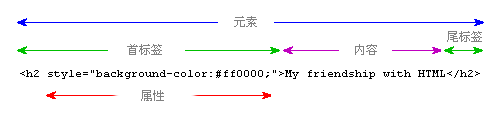
\includegraphics[scale=0.5]{htmlelements.png}
\end{figure}



\chapter{Varieties}


HTML attributes are generally classed as required attributes, optional attributes, standard attributes, and event attributes. Usually the required and optional attributes modify specific HTML elements, while the standard attributes can be applied to most HTML elements. Event attributes, added in HTML version 4, allow an element to specify scripts to be run under specific circumstances.



\section{Required and optional HTML attributes}


\subsection{Used by one tag}


\begin{compactitem}
\item <applet>: code, object
\item <area>: nohref
\item <body>: alink, background, link, text, vlink
\item <dir>: dir
\item <form>: accept-charset, action, enctype, method
\item <frame>: noresize
\item <head>: profile
\item <hr>: noshade
\item <html>: xmlns
\item <img>: ismap
\item <input>: checked, maxlength
\item <label>: for
\item <meta>: content, http-equiv, scheme
\item <object>: classid, codetag, data, declare, standby
\item <ol>: start
\item <option>: selected
\item <param>: valuetype
\item <script>: defer, xml:space
\item <select>: multiple
\item <table>: cellpadding, cellspacing, frame, rules, summary
\item <td>: headers
\end{compactitem}





\subsection{Used by two tags}

\begin{compactitem}
\item <a> and <area>:

	\begin{compactitem}
	\item coords — coordinates of an area or a link within it.
	\item shape — shape of an area or a link within it. Values: default, rect, circle, poly.
	\end{compactitem}

\item <a> and <link>:

	\begin{compactitem}
	\item hreflang — Language code of the linked document. (a, link)
	\item rel — Nature of the linked document (relative to the page currently displayed). Free text for a, but link uses a set of terms (alternate, appendix, bookmark, chapter, contents, copyright, glossary, help, home, index, next, prev, section, start, stylesheet, subsection).
	\item rev — Nature of the currently displayed page (relative to the linked document). Varies for a and link as for rel.
	\end{compactitem}

\item <applet> and <object>:

	\begin{compactitem}
	\item archive — archive URL(s) (applet, object)
	\item codebase — base URL (applet, object)
	\end{compactitem}
	
\item <basefont> and <font>:
	
	\begin{compactitem}
	\item color — text color (deprecated) (basefont, font)
	\item face — font family (deprecated) (basefont, font)
	\end{compactitem}
	
\item <col> and <colgroup>:
	
	\begin{compactitem}
	\item span — number of columns spanned (col, colgroup)
	\end{compactitem}
	
\item <del> and <ins>:
	
	\begin{compactitem}
	\item datetime — date and time of text deletion or insertion.
	\end{compactitem}
	
\item <form> and <input>:
	
	\begin{compactitem}
	\item accept — types of files accepted when uploading form or input
	\end{compactitem}
	
\item <frame> and <iframe>:
	
	\begin{compactitem}
	\item frameborder — value (0 or 1) specifies whether to display a border around the frame or iframe.
	\item marginheight — top and bottom margins in pixels around the frame or iframe.
	\item scrolling — value (yes, no, auto) specifies whether to display scroll bars around the frame or iframe.
	\item marginwidth — left and right margins in pixels around the frame or iframe.
	\end{compactitem}
	
\item <frameset> and <textarea>:
	
	\begin{compactitem}
	\item cols — number of visible columns in frameset or cols (some variation)
	\item rows — number of visible rows in frameset or rows (some variation)
	\end{compactitem}
	
\item <img> and <object>:
	
	\begin{compactitem}
	\item usemap — specifies name of a map tag to use with img -or- URL of an image-map to use with object.
	\end{compactitem}
	
\item <input> and <textarea>:

	\begin{compactitem}
	\item readonly — specifies read-only text for input and textarea.
	\end{compactitem}
	
\item <link> and <style>:

	\begin{compactitem}
	\item media — specifies display device for link and style. Values: all, aural, braille, handheld, print, projection, screen, tty, TV.
	\end{compactitem}
	
\item <optgroup> and <option>:

	\begin{compactitem}
	\item label — description text for an optgroup or option.
	\end{compactitem}
	
\item <td> and <th>:

	\begin{compactitem}
	\item abbr — abbreviated version of a table cell or header.
	\item axis — category name for a table cell or header.
	\item colspan — number of columns spanned by a table cell or header.
	\item nowrap — (deprecated) prevents wrapping of a table cell or header.
	\item rowspan — number of rows spanned by a table cell or header.
	\item scope — no effect on normal browser display, but marks a table cell or header as a logical header for other cells. Values: col, colgroup, row, rowgroup.
	\end{compactitem}
	
\end{compactitem}








\subsection{Used by multiple tags}

\begin{compactitem}
\item align — applet, col, colgroup, object, tbody, td, tfoot, th, thead, also (deprecated) in caption, div, h1 to h6, hr, iframe, img, input, legend, p, table
\item alt — applet, area, img, input
\item bgcolor — body, table, td, th, bgcolor
\item border — img, object, table
\item char — char, <colgroup>, <tbody>, <td>, <tfoot>, <th>, <thead>, <tr>
\item charoff — col, colgroup, tbody, td, tfoot, th, thead, tr
\item charset — a, link, script
\item cite — blockquote, del, ins, q
\item compact — dir, menu, ol, ul
\item disabled — button, input, optgroup, option, select, textarea
\item height - applet, iframe, img, object — also (deprecated) td, th
\item href — a, area, base, link
\item hspace — applet, object — also (deprecated) img
\item longdesc — frame, iframe, img
\item name — a, applet, button, form, frame, iframe, input, map, meta, object, param, select, textarea
\item size — basefont, font, hr, input, select
\item src — frame, iframe, img, input, script)
\item target — <a>, area, base, form, link
\item type — button, input, li, link, object, ol, param, script, style, type
\item valign — col, colgroup, tbody, td, tfoot, th, thead, tr
\item value — button, input, li, option, param
\item vspace — applet, img, object
\item width — applet, col, colgroup, hr, iframe, img, object, pre, table, td, th
\end{compactitem}







\chapter{Standard attributes}



\begin{longtable}{|l|l|l|l|l|l|l|l|l|l|}
\multicolumn{10}{r}{...}
%\tabularnewline\hline
\endhead
\hline

%\tabularnewline\hline
\endfirsthead
\multicolumn{10}{r}{...}
\endfoot
%\tabularnewline\hline
\endlastfoot
\hline
<param>		&id	    &		 &		 &		&	 &	 	&		  &			&		\\
\hline
<head>		&	    &		 &		 &		& dir & 	lang	& xml:lang & 			&		 \\
\hline
<html>		&	    &		 &		 &		& dir & 	lang	& xml:lang & 			&		 \\
\hline
<meta>		&	    &		 &		 &		& dir & 	lang	& xml:lang & 			&		 \\
\hline
<title>		&	    &		 &		 &		& dir & 	lang	& xml:lang & 			&		 \\
\hline
<style>		&	    &		 &		 &	title	& dir & 	lang	& xml:lang & 			&		 \\
\hline
<applet>		&	id &	class &	style &	title &  	 & 		& 	 	   & 			&		 \\
\hline
<br>			&	id &	class &	style &	title &  	 & 		& 	 	   & 			&		 \\
\hline
<frame>		&	id &	class &	style &	title &  	 & 		& 	 	   & 			&		 \\
\hline
<frameset>	&	id &	class &	style &	title &  	 & 		& 	 	   & 			&		 \\
\hline
<iframe>		&	id &	class &	style &	title &  	 & 		& 	 	   & 			&		 \\
\hline
<basefont>	&	id &	class &	style &	title & dir & 	lang	& 	 & 			&		 \\
\hline
<center>		&	id &	class &	style &	title & dir & 	lang	& 	 & 			&		 \\
\hline
<dir>		&	id &	class &	style &	title & dir & 	lang	& 	 & 			&		 \\
\hline
<font>		&	id &	class &	style &	title & dir & 	lang	& 	 & 			&		 \\
\hline
<menu>		&	id &	class &	style &	title & dir & 	lang	& 	 & 			&		 \\
\hline
<s>			&	id &	class &	style &	title & dir & 	lang	& 	 & 			&		 \\
\hline
<strike>		&	id &	class &	style &	title & dir & 	lang	& 	 & 			&		 \\
\hline
<u>			&	id &	class &	style &	title & dir & 	lang	& 	 & 			&		 \\
\hline
<abbr>		&	id &	class &	style &	title & dir & 	lang	& xml:lang & 			&		 \\
\hline
<acronym>	&	id &	class &	style &	title & dir & 	lang	& xml:lang & 			&		 \\
\hline
<address>	&	id &	class &	style &	title & dir & 	lang	& xml:lang & 			&		 \\
\hline
<b>			&	id &	class &	style &	title & dir & 	lang	& xml:lang & 			&		 \\
\hline
<big>		&	id &	class &	style &	title & dir & 	lang	& xml:lang & 			&		 \\
\hline
<blockquote>	&	id &	class &	style &	title & dir & 	lang	& xml:lang & 			&		 \\
\hline
<body>		&	id &	class &	style &	title & dir & 	lang	& xml:lang & 			&		 \\
\hline
<caption>		&	id &	class &	style &	title & dir & 	lang	& xml:lang & 			&		 \\
\hline
<cite>		&	id &	class &	style &	title & dir & 	lang	& xml:lang & 			&		 \\
\hline
<code>		&	id &	class &	style &	title & dir & 	lang	& xml:lang & 			&		 \\
\hline
<col>		&	id &	class &	style &	title & dir & 	lang	& xml:lang & 			&		 \\
\hline
<colgroup>	&	id &	class &	style &	title & dir & 	lang	& xml:lang & 			&		 \\
\hline
<dd>		&	id &	class &	style &	title & dir & 	lang	& xml:lang & 			&		 \\
\hline
<del>		&	id &	class &	style &	title & dir & 	lang	& xml:lang & 			&		 \\
\hline
<dfn>		&	id &	class &	style &	title & dir & 	lang	& xml:lang & 			&		 \\
\hline
<div>		&	id &	class &	style &	title & dir & 	lang	& xml:lang & 			&		 \\
\hline
<dl>			&	id &	class &	style &	title & dir & 	lang	& xml:lang & 			&		 \\
\hline
<dt>			&	id &	class &	style &	title & dir & 	lang	& xml:lang & 			&		 \\
\hline
<em>		&	id &	class &	style &	title & dir & 	lang	& xml:lang & 			&		 \\
\hline
<fieldset>	&	id &	class &	style &	title & dir & 	lang	& xml:lang & 			&		 \\
\hline
<form>		&	id &	class &	style &	title & dir & 	lang	& xml:lang & 			&		 \\
\hline
<hn>		&	id &	class &	style &	title & dir & 	lang	& xml:lang & 			&		 \\
\hline
<h1> to <h6>	&	id &	class &	style &	title & dir & 	lang	& xml:lang & 			&		 \\
\hline
<i>			&	id &	class &	style &	title & dir & 	lang	& xml:lang & 			&		 \\
\hline
<img>		&	id &	class &	style &	title & dir & 	lang	& xml:lang & 			&		 \\
\hline
<ins>		&	id &	class &	style &	title & dir & 	lang	& xml:lang & 			&		 \\
\hline
<kbd>		&	id &	class &	style &	title & dir & 	lang	& xml:lang & 			&		 \\
\hline
<li>			&	id &	class &	style &	title & dir & 	lang	& xml:lang & 			&		 \\
\hline
<link>		&	id &	class &	style &	title & dir & 	lang	& xml:lang & 			&		 \\
\hline
<map>		&	id &	class &	style &	title & dir & 	lang	& xml:lang & 			&		 \\
\hline
<noframes>	&	id &	class &	style &	title & dir & 	lang	& xml:lang & 			&		 \\
\hline
<noscript>	&	id &	class &	style &	title & dir & 	lang	& xml:lang & 			&		 \\
\hline
<ol>			&	id &	class &	style &	title & dir & 	lang	& xml:lang & 			&		 \\
\hline
<optgroup>	&	id &	class &	style &	title & dir & 	lang	& xml:lang & 			&		 \\
\hline
<option>		&	id &	class &	style &	title & dir & 	lang	& xml:lang & 			&		 \\
\hline
<p>			&	id &	class &	style &	title & dir & 	lang	& xml:lang & 			&		 \\
\hline
<pre>		&	id &	class &	style &	title & dir & 	lang	& xml:lang & 			&		 \\
\hline
<q>			&	id &	class &	style &	title & dir & 	lang	& xml:lang & 			&		 \\
\hline
<samp>		&	id &	class &	style &	title & dir & 	lang	& xml:lang & 			&		 \\
\hline
<small>		&	id &	class &	style &	title & dir & 	lang	& xml:lang & 			&		 \\
\hline
<span>		&	id &	class &	style &	title & dir & 	lang	& xml:lang & 			&		 \\
\hline
<strong>		&	id &	class &	style &	title & dir & 	lang	& xml:lang & 			&		 \\
\hline
<sub>		&	id &	class &	style &	title & dir & 	lang	& xml:lang & 			&		 \\
\hline
<sup>		&	id &	class &	style &	title & dir & 	lang	& xml:lang & 			&		 \\
\hline
<table>		&	id &	class &	style &	title & dir & 	lang	& xml:lang & 			&		 \\
\hline
<tbody>		&	id &	class &	style &	title & dir & 	lang	& xml:lang & 			&		 \\
\hline
<td>			&	id &	class &	style &	title & dir & 	lang	& xml:lang & 			&		 \\
\hline
<tfoot>		&	id &	class &	style &	title & dir & 	lang	& xml:lang & 			&		 \\
\hline
<th>			&	id &	class &	style &	title & dir & 	lang	& xml:lang & 			&		 \\
\hline
<thead>		&	id &	class &	style &	title & dir & 	lang	& xml:lang & 			&		 \\
\hline
<tr>			&	id &	class &	style &	title & dir & 	lang	& xml:lang & 			&		 \\
\hline
<tt>	          	&	id &	class &	style &	title & dir & 	lang	& xml:lang & 			&		 \\
\hline
<ul>            	&	id &	class &	style &	title & dir & 	lang	& xml:lang & 			&		 \\
\hline
<var>	   	&	id &	class &	style &	title & dir & 	lang	& xml:lang & 			&		 \\
\hline
<label>	   	&	id &	class &	style &	title & dir & 	lang	& xml:lang & accesskey &  		  \\
\hline
<legend>	   	&	id &	class &	style &	title & dir & 	lang	& xml:lang & accesskey & 		  \\
\hline
<object>	   	&	id &	class &	style &	title & dir & 	lang	& xml:lang & 			& tabindex \\
\hline
<select>	   	&	id &	class &	style &	title & dir & 	lang	& xml:lang & 			& tabindex \\
\hline
<a>	           	&	id &	class &	style &	title & dir & 	lang	& xml:lang & accesskey & tabindex \\
\hline
<area>	   	&	id &	class &	style &	title & dir & 	lang	& xml:lang & accesskey & tabindex \\
\hline
<button>	   	&	id &	class &	style &	title & dir & 	lang	& xml:lang & accesskey & tabindex \\
\hline
<input>	   	&	id &	class &	style &	title & dir & 	lang	& xml:lang & accesskey & tabindex \\
\hline
<textarea> 	&	id &	class &	style &	title & dir & 	lang	& xml:lang & accesskey & tabindex \\
\hline
\end{longtable}






\section{Event attributes}


\zihao{8}

%\begin{sidewaystable}{!h}
\begin{longtable}{|p{18pt}|p{15pt}|p{15pt}|p{10pt}|p{16pt}|p{16pt}|p{16pt}|p{16pt}|p{16pt}|p{16pt}|p{16pt}|p{16pt}|p{16pt}|p{16pt}|p{16pt}|p{16pt}|p{16pt}|p{16pt}|}
\multicolumn{18}{r}{...}
%\tabularnewline\hline
\endhead
\hline

%\tabularnewline\hline
\endfirsthead
\multicolumn{18}{r}{...}
\endfoot
%\tabularnewline\hline
\endlastfoot
\hline
<frameset>	& onload	& onunload &	&& 		&  &  &  &  &  &  &  &  &  & & & \\				
\hline													
<body>		& onload	& onunload &	&onclick	& ondblclick & onmousedown & onmousemove & onmouseout & onmouseover & onmouseup & onkeydown & onkeypress & onkeyup & & & & \\ 		
\hline
<abbr>		&	&	&	& onclick	& ondblclick & onmousedown & onmousemove & onmouseout & onmouseover & onmouseup & onkeydown & onkeypress & onkeyup & & & & \\				
\hline
<acronym>	&	&	&	& onclick	& ondblclick & onmousedown & onmousemove & onmouseout & onmouseover & onmouseup & onkeydown & onkeypress & onkeyup & & & & \\				
\hline
<address>	&	&	&	& onclick	& ondblclick & onmousedown & onmousemove & onmouseout & onmouseover & onmouseup & onkeydown & onkeypress & onkeyup & & & & \\				
\hline
<b>			&	&	&	& onclick	& ondblclick & onmousedown & onmousemove & onmouseout & onmouseover & onmouseup & onkeydown & onkeypress & onkeyup & & & & \\
\hline
<big>		&	&	&	& onclick	& ondblclick & onmousedown & onmousemove & onmouseout & onmouseover & onmouseup & onkeydown & onkeypress & onkeyup & & & & \\
\hline
<blockquote>	&	&	&	& onclick	& ondblclick & onmousedown & onmousemove & onmouseout & onmouseover & onmouseup & onkeydown & onkeypress & onkeyup & & & & \\
\hline
<caption>		&	&	&	& onclick	& ondblclick & onmousedown & onmousemove & onmouseout & onmouseover & onmouseup & onkeydown & onkeypress & onkeyup & & & & \\
\hline
<center>		&	&	&	& onclick	& ondblclick & onmousedown & onmousemove & onmouseout & onmouseover & onmouseup & onkeydown & onkeypress & onkeyup & & & & \\
\hline
<cite>		&	&	&	& onclick	& ondblclick & onmousedown & onmousemove & onmouseout & onmouseover & onmouseup & onkeydown & onkeypress & onkeyup & & & & \\
\hline
<code>		&	&	&	& onclick	& ondblclick & onmousedown & onmousemove & onmouseout & onmouseover & onmouseup & onkeydown & onkeypress & onkeyup & & & & \\
\hline
<col>		&	&	&	& onclick	& ondblclick & onmousedown & onmousemove & onmouseout & onmouseover & onmouseup & onkeydown & onkeypress & onkeyup & & & & \\
\hline
<colgroup>	&	&	&	& onclick	& ondblclick & onmousedown & onmousemove & onmouseout & onmouseover & onmouseup & onkeydown & onkeypress & onkeyup & & & & \\
\hline
<dd>		&	&	&	& onclick	& ondblclick & onmousedown & onmousemove & onmouseout & onmouseover & onmouseup & onkeydown & onkeypress & onkeyup & & & & \\
\hline
<del>		&	&	&	& onclick	& ondblclick & onmousedown & onmousemove & onmouseout & onmouseover & onmouseup & onkeydown & onkeypress & onkeyup & & & & \\
\hline
<dfn>		&	&	&	& onclick	& ondblclick & onmousedown & onmousemove & onmouseout & onmouseover & onmouseup & onkeydown & onkeypress & onkeyup & & & & \\
\hline
<dir>		&	&	&	& onclick	& ondblclick & onmousedown & onmousemove & onmouseout & onmouseover & onmouseup & onkeydown & onkeypress & onkeyup & & & & \\
\hline
<div>		&	&	&	& onclick	& ondblclick & onmousedown & onmousemove & onmouseout & onmouseover & onmouseup & onkeydown & onkeypress & onkeyup & & & & \\
\hline
<dl>			&	&	&	& onclick	& ondblclick & onmousedown & onmousemove & onmouseout & onmouseover & onmouseup & onkeydown & onkeypress & onkeyup & & & & \\
\hline
<dt>			&	&	&	& onclick	& ondblclick & onmousedown & onmousemove & onmouseout & onmouseover & onmouseup & onkeydown & onkeypress & onkeyup & & & & \\
\hline
<em>		&	&	&	& onclick	& ondblclick & onmousedown & onmousemove & onmouseout & onmouseover & onmouseup & onkeydown & onkeypress & onkeyup & & & & \\
\hline
<fieldset>	&	&	&	& onclick	& ondblclick & onmousedown & onmousemove & onmouseout & onmouseover & onmouseup & onkeydown & onkeypress & onkeyup & & & & \\
\hline
<h1>to<h6>	&	&	&	& onclick	& ondblclick & onmousedown & onmousemove & onmouseout & onmouseover & onmouseup & onkeydown & onkeypress & onkeyup & & & & \\
\hline
<hr>			&	&	&	& onclick	& ondblclick & onmousedown & onmousemove & onmouseout & onmouseover & onmouseup & onkeydown & onkeypress & onkeyup & & & & \\
\hline
<i>			&	&	&	& onclick	& ondblclick & onmousedown & onmousemove & onmouseout & onmouseover & onmouseup & onkeydown & onkeypress & onkeyup & & & & \\
\hline
<ins>		&	&	&	& onclick	& ondblclick & onmousedown & onmousemove & onmouseout & onmouseover & onmouseup & onkeydown & onkeypress & onkeyup & & & & \\
\hline
<kbd>		&	&	&	& onclick	& ondblclick & onmousedown & onmousemove & onmouseout & onmouseover & onmouseup & onkeydown & onkeypress & onkeyup & & & & \\
\hline
<legend>		&	&	&	& onclick	& ondblclick & onmousedown & onmousemove & onmouseout & onmouseover & onmouseup & onkeydown & onkeypress & onkeyup & & & & \\
\hline
<li>			&	&	&	& onclick	& ondblclick & onmousedown & onmousemove & onmouseout & onmouseover & onmouseup & onkeydown & onkeypress & onkeyup & & & & \\
\hline
<link>		&	&	&	& onclick	& ondblclick & onmousedown & onmousemove & onmouseout & onmouseover & onmouseup & onkeydown & onkeypress & onkeyup & & & & \\
\hline
<map>		&	&	&	& onclick	& ondblclick & onmousedown & onmousemove & onmouseout & onmouseover & onmouseup & onkeydown & onkeypress & onkeyup & & & & \\
\hline
<menu>		&	&	&	& onclick	& ondblclick & onmousedown & onmousemove & onmouseout & onmouseover & onmouseup & onkeydown & onkeypress & onkeyup & & & & \\
\hline
<noframes>	&	&	&	& onclick	& ondblclick & onmousedown & onmousemove & onmouseout & onmouseover & onmouseup & onkeydown & onkeypress & onkeyup & & & & \\
\hline
<noscript>	&	&	&	& onclick	& ondblclick & onmousedown & onmousemove & onmouseout & onmouseover & onmouseup & onkeydown & onkeypress & onkeyup & & & & \\
\hline
<ol>			&	&	&	& onclick	& ondblclick & onmousedown & onmousemove & onmouseout & onmouseover & onmouseup & onkeydown & onkeypress & onkeyup & & & & \\
\hline
<optgroup>	&	&	&	& onclick	& ondblclick & onmousedown & onmousemove & onmouseout & onmouseover & onmouseup & onkeydown & onkeypress & onkeyup & & & & \\
\hline
<option>		&	&	&	& onclick	& ondblclick & onmousedown & onmousemove & onmouseout & onmouseover & onmouseup & onkeydown & onkeypress & onkeyup & & & & \\
\hline
<p>			&	&	&	& onclick	& ondblclick & onmousedown & onmousemove & onmouseout & onmouseover & onmouseup & onkeydown & onkeypress & onkeyup & & & & \\
\hline
<pre>		&	&	&	& onclick	& ondblclick & onmousedown & onmousemove & onmouseout & onmouseover & onmouseup & onkeydown & onkeypress & onkeyup & & & & \\
\hline
<q>			&	&	&	& onclick	& ondblclick & onmousedown & onmousemove & onmouseout & onmouseover & onmouseup & onkeydown & onkeypress & onkeyup & & & & \\
\hline
<s>			&	&	&	& onclick	& ondblclick & onmousedown & onmousemove & onmouseout & onmouseover & onmouseup & onkeydown & onkeypress & onkeyup & & & & \\
\hline
<samp>		&	&	&	& onclick	& ondblclick & onmousedown & onmousemove & onmouseout & onmouseover & onmouseup & onkeydown & onkeypress & onkeyup & & & & \\
\hline
<small>		&	&	&	& onclick	& ondblclick & onmousedown & onmousemove & onmouseout & onmouseover & onmouseup & onkeydown & onkeypress & onkeyup & & & & \\
\hline
<span>		&	&	&	& onclick	& ondblclick & onmousedown & onmousemove & onmouseout & onmouseover & onmouseup & onkeydown & onkeypress & onkeyup & & & & \\
\hline
<strike>		&	&	&	& onclick	& ondblclick & onmousedown & onmousemove & onmouseout & onmouseover & onmouseup & onkeydown & onkeypress & onkeyup & & & & \\
\hline
<strong>		&	&	&	& onclick	& ondblclick & onmousedown & onmousemove & onmouseout & onmouseover & onmouseup & onkeydown & onkeypress & onkeyup & & & & \\
\hline
<sub>		&	&	&	& onclick	& ondblclick & onmousedown & onmousemove & onmouseout & onmouseover & onmouseup & onkeydown & onkeypress & onkeyup & & & & \\
\hline
<sup>		&	&	&	& onclick	& ondblclick & onmousedown & onmousemove & onmouseout & onmouseover & onmouseup & onkeydown & onkeypress & onkeyup & & & & \\
\hline
<table>		&	&	&	& onclick	& ondblclick & onmousedown & onmousemove & onmouseout & onmouseover & onmouseup & onkeydown & onkeypress & onkeyup & & & & \\
\hline
<tbody>		&	&	&	& onclick	& ondblclick & onmousedown & onmousemove & onmouseout & onmouseover & onmouseup & onkeydown & onkeypress & onkeyup & & & & \\
\hline
<td>			&	&	&	& onclick	& ondblclick & onmousedown & onmousemove & onmouseout & onmouseover & onmouseup & onkeydown & onkeypress & onkeyup & & & & \\
\hline
<tfoot>		&	&	&	& onclick	& ondblclick & onmousedown & onmousemove & onmouseout & onmouseover & onmouseup & onkeydown & onkeypress & onkeyup & & & & \\
\hline
<th>			&	&	&	& onclick	& ondblclick & onmousedown & onmousemove & onmouseout & onmouseover & onmouseup & onkeydown & onkeypress & onkeyup & & & & \\
\hline
<thead>		&	&	&	& onclick	& ondblclick & onmousedown & onmousemove & onmouseout & onmouseover & onmouseup & onkeydown & onkeypress & onkeyup & & & & \\
\hline
<tr>			&	&	&	& onclick	& ondblclick & onmousedown & onmousemove & onmouseout & onmouseover & onmouseup & onkeydown & onkeypress & onkeyup & & & & \\
\hline
<tt>			&	&	&	& onclick	& ondblclick & onmousedown & onmousemove & onmouseout & onmouseover & onmouseup & onkeydown & onkeypress & onkeyup & & & & \\
\hline
<u>			&	&	&	& onclick	& ondblclick & onmousedown & onmousemove & onmouseout & onmouseover & onmouseup & onkeydown & onkeypress & onkeyup & & & & \\
\hline
<ul>			&	&	&	& onclick	& ondblclick & onmousedown & onmousemove & onmouseout & onmouseover & onmouseup & onkeydown & onkeypress & onkeyup & & & & \\
\hline
<var>		&	&	&	& onclick	& ondblclick & onmousedown & onmousemove & onmouseout & onmouseover & onmouseup & onkeydown & onkeypress & onkeyup & & & & \\
\hline
<img>		&	&	&onabort	& onclick	& ondblclick & onmousedown & onmousemove & onmouseout & onmouseover & onmouseup & onkeydown & onkeypress & onkeyup & & & & \\
\hline
<a>			&	&	&	& onclick	& ondblclick & onmousedown & onmousemove & onmouseout & onmouseover & onmouseup & onkeydown & onkeypress & onkeyup &onblur &onfocus & & \\				
\hline
<area>		&	&	&	& onclick	& ondblclick & onmousedown & onmousemove & onmouseout & onmouseover & onmouseup & onkeydown & onkeypress & onkeyup &onblur &onfocus & & \\				
\hline
<button>		&	&	&	& onclick	& ondblclick & onmousedown & onmousemove & onmouseout & onmouseover & onmouseup & onkeydown & onkeypress & onkeyup &onblur &onfocus & & \\				
\hline
<form>		&	&	&	& onclick	& ondblclick & onmousedown & onmousemove & onmouseout & onmouseover & onmouseup & onkeydown & onkeypress & onkeyup &onblur &onfocus & & \\				
\hline
<label>		&	&	&	& onclick	& ondblclick & onmousedown & onmousemove & onmouseout & onmouseover & onmouseup & onkeydown & onkeypress & onkeyup &onblur &onfocus & & \\				
\hline
<select>		&	&	&	& onclick	& ondblclick & onmousedown & onmousemove & onmouseout & onmouseover & onmouseup & onkeydown & onkeypress & onkeyup &onblur &onfocus &onchange & \\				
\hline
<input>		&	&	&	& onclick	& ondblclick & onmousedown & onmousemove & onmouseout & onmouseover & onmouseup & onkeydown & onkeypress & onkeyup &onblur &onfocus &onchange &onselect \\				
\hline
<textarea>	&	&	&	& onclick	& ondblclick & onmousedown & onmousemove & onmouseout & onmouseover & onmouseup & onkeydown & onkeypress & onkeyup &onblur &onfocus &onchange &onselect \\				
\hline
\end{longtable}
%\end{sidewaystable}

\zihao{5}


下面列出了所有 HTML 和 XHTML 标签支持的标准属性,仅有少数例外。

\section{Core Attributes}



以下标签不提供下面的属性:base、head、html、meta、param、script、style 以及 title 元素。

\begin{table}[!h]
\centering
\caption{核心属性 (Core Attributes)}
\begin{tabular}{|l|l|l|}
\hline
属性		&值			&描述\\
\hline
class	&classname	&规定元素的类名(classname)\\
\hline
id		&id			&规定元素的唯一 id\\
\hline
style	&style\_definition&	规定元素的行内样式(inline style)\\
\hline
title		&text		&规定元素的额外信息(可在工具提示中显示)\\
\hline
\end{tabular}
\end{table}


\section{Language Attributes}


以下标签不提供下面的属性:base、br、frame、frameset、hr、iframe、param 以及 script 元素。

\begin{table}[!h]
\centering
\caption{语言属性 (Language Attributes)}
\begin{tabular}{|l|l|l|}
\hline
属性		&值		&描述\\
\hline
dir		&ltr | rtl	&设置元素中内容的文本方向。\\
\hline
lang		&language\_code&	设置元素中内容的语言代码。\\
\hline
xml:lang	&language\_code&	设置 XHTML 文档中元素内容的语言代码。\\
\hline
\end{tabular}
\end{table}

lang 属性应用于几乎所有的 XHTML 元素,它定义元素内部的内容的所用语言的类型。

如果在某元素中使用 lang 属性,就必须添加额外的 xml:lang,像这样:

\begin{lstlisting}[language=HTML]
<div lang="no" xml:lang="no">test</div>
\end{lstlisting}



\section{Keyboard Attributes}


\begin{table}[!h]
\centering
\caption{键盘属性 (Keyboard Attributes)}
\begin{tabular}{|l|l|l|}
\hline
属性			&值			&描述\\
\hline
accesskey	&character	&设置访问元素的键盘快捷键。\\
\hline
tabindex		&number		&设置元素的 Tab 键控制次序。\\
\hline
\end{tabular}
\end{table}



































































\part{HTML Events}


HTML 4 的新特性之一是可以使 HTML 事件触发浏览器中的行为,比方说当用户点击某个 HTML 元素时启动一段 JavaScript。

在现代浏览器中都内置有大量的事件处理器。这些处理器会监视特定的条件或用户行为,例如鼠标单击或浏览器窗口中完成加载某个图像。通过使用客户端的 JavaScript,可以将某些特定的事件处理器作为属性添加给特定的标签,并可以在事件发生时执行一个或多个 JavaScript 命令或函数。

事件处理器的值是一个或一系列以分号隔开的 Javascript 表达式、方法和函数调用,并用引号引起来。当事件发生时,浏览器会执行这些代码。例如,当用户把鼠标移动到一个超链接时,会启动一个 JavaScript 函数。支持 JavaScript 的浏览器支持 <a> 标签中的一个特殊的 "mouse over"事件处理器 - 被称为 onmouseover 来完成这项工作:


\begin{lstlisting}[language=HTML]
     <a href="/index.html" onmouseover="alert('Welcome');return false"></a>
\end{lstlisting}

下面的表格提供了标准的事件属性,可以把它们插入 HTML/XHTML 元素中,以定义事件行为。





\chapter{Window Events}

仅在 body 和 frameset 元素中有效。


\begin{table}[!h]
\centering
\caption{窗口事件 (Window Events)}
\begin{tabular}{|l|l|l|}
\hline
属性		&值		&描述\\
\hline
onload	&脚本	&当文档被载入时执行脚本\\
\hline
onunload	&脚本	&当文档被卸下时执行脚本\\
\hline
\end{tabular}
\end{table}








\chapter{Form Element Events}

仅在表单元素中有效。


\begin{table}[!h]
\centering
\caption{表单元素事件 (Form Element Events)}
\begin{tabular}{|l|l|l|}
\hline
属性		&值		&描述\\
\hline
onchange&脚本	&当元素改变时执行脚本\\
\hline
onsubmit	&脚本	&当表单被提交时执行脚本\\
\hline
onreset	&脚本	&当表单被重置时执行脚本\\
\hline
onselect	&脚本	&当元素被选取时执行脚本\\
\hline
onblur	&脚本	&当元素失去焦点时执行脚本\\
\hline
onfocus	&脚本	&当元素获得焦点时执行脚本\\
\hline
\end{tabular}
\end{table}








\chapter{Image Events}

该属性可用于 img 元素:

\begin{table}[!h]
\centering
\caption{图像事件 (Image Events)}
\begin{tabular}{|l|l|l|}
\hline
属性		&值		&描述\\
\hline
onabort	&脚本	&当图像加载中断时执行脚本\\
\hline
\end{tabular}
\end{table}




\chapter{Keyboard Events}


在下列元素中无效:base、bdo、br、frame、frameset、head、html、iframe、meta、param、script、style 以及 title 元素。

\begin{table}[!h]
\centering
\caption{键盘事件 (Keyboard Events)}
\begin{tabular}{|l|l|l|}
\hline
属性			&值	&描述\\
\hline
onkeydown	&脚本	&当键盘被按下时执行脚本\\
\hline
onkeypress	&脚本	&当键盘被按下后又松开时执行脚本\\
\hline
onkeyup		&脚本	&当键盘被松开时执行脚本\\
\hline
\end{tabular}
\end{table}







\chapter{Mouse Events}

在下列元素中无效:base、bdo、br、frame、frameset、head、html、iframe、meta、param、script、style 以及 title 元素。

\begin{table}[!h]
\centering
\caption{鼠标事件 (Mouse Events)}
\begin{tabular}{|l|l|l|}
\hline
属性			&值		&描述\\
\hline
onclick		&脚本	&当鼠标被单击时执行脚本\\
\hline
ondblclick	&脚本	&当鼠标被双击时执行脚本\\
\hline
onmousedown	&脚本	&当鼠标按钮被按下时执行脚本\\
\hline
onmousemove	&脚本	&当鼠标指针移动时执行脚本\\
\hline
onmouseout	&脚本	&当鼠标指针移出某元素时执行脚本\\
\hline
onmouseover	&脚本	&当鼠标指针悬停于某元素之上时执行脚本\\
\hline
onmouseup	&脚本	&当鼠标按钮被松开时执行脚本\\
\hline
\end{tabular}
\end{table}





















\part{HTML Style}

很多标签都可以用来改变文本的外观,并为文本关联其隐藏的含义。总地来说,这些标签可以分成两类:基于内容的样式(content-based style)和物理样式(physical style)。

同时,W3C 为级联样式表(CSS)指定的标准现在已被绝大多数浏览器所支持\footnote{自HTML4.0开始,所有的格式化代码均可移出 HTML 文档,然后移入一个独立的外部样式表。},它提供了一种允许作者控制文档文本外观和布局的更为全面的方法。

\chapter{Content-based Style}


基于内容的样式标签会告诉浏览器它所包含的文本具有特定的含义、上下文或者用法。然后浏览器就会把与该含义、上下文或者用法一致的格式应用在文本上。请注意这里面的区别。基于内容的标签赋予含义,而不是格式化。因此,它们对于自动处理来说非常重要;计算机并不关心文档的外观如何。

因为字体样式是通过语义线索来指定的,因此浏览器可以为用户选择一种合适的显示样式。由于不同地点的样式各种各样,所以使用基于内容的样式可以帮助用户确保自己的文档对广大范围的读者来说都是有意义的。这一点在专门供那些盲人和残疾人所使用的浏览器上显得尤其重要,因为他们的显示选项可能和我们传统的文本根本不同,或者在某方面具有非常大的局限性。

当前的 HTML 和 XHTML 标准并没有为每一个基于内容的标签都定义一种格式;它们仅仅规定必须用与文档中普通文本不同的方式来显示基于内容的样式。标准甚至没有要求这些基于内容的样式彼此之间都要用不同的方式显示。在实际应用中,你可能会发现很多这样的标签和传统的印刷有着非常明显的关系,它们有着相似的含义和显示样式,而且在多数浏览器中都以相同的样式和字体来显示。

使用 HTML/XHTML 基于内容的样式标签时要遵从一些规则,因为仅仅是简单地想想文本该如何显示,而不必知道这些文本的含义是什么,是十分容易的。一旦你开始使用基于内容的样式之后,文档将会更加一致,而且可以更好地帮助执行自动搜索和内容编辑。这些标签是:

\begin{compactitem}
\item <abbr>
\item <acronym>
\item <cite>
\item <code>
\item <dfn>
\item <em>
\item <kbd>
\item <samp>
\item <strong>
\item <var>
\end{compactitem}


\chapter{Physical Style}


在讨论基于内容的样式标签时,我们经常用到“意图”这个词。这是因为由标签传达的含义比浏览器显示文本的方式更为重要。然而,在某些情况下,可能是出于合法性或者版权等方面的原因的考虑,用户希望文本以某种特殊的方式来显示(例如斜体或加粗)。在这种情况下,就可以对文本使用物理样式。

虽然其他文字处理系统的趋势是精确地控制样式和外观,但是在使用 HTML 或 XHTML 时,除非极少情况下,都应该避免使用物理标签。应当尽可能地向浏览器提供上下文信息,并使用基于内容的样式。尽管现在浏览器不过是以斜体或者粗体字来显示这些文本,但是将来的浏览器和各种文档生成工具可能会以非常有创见的方式来利用这些基于内容的样式。


当前的 HTML/XHTML 标准一共提供了 9 种物理样式,包括粗体(bold)、斜体(italic)、等宽(monospaced)、下划线(underlined)、删除线(strikethrough)、放大(larger)、缩小(smaller)、上标(superscripted)和下标(subscripted)文本。这些标签\footnote{记住这些物理样式标签对紧接的文本产生的强烈效果。要实现在整个文档范围内对文本显示的全面控制,应该使用样式表。}是:

\begin{compactitem}
\item <b>
\item <big>
\item <i>
\item <s>
\item <small>
\item <strike>
\item <sub>
\item <sup>
\item <tt>
\end{compactitem}

\chapter{HTML CSS}

当浏览器读到一个样式表,它就会按照这个样式表来对文档进行格式化,从而达到精确地控制页面设置与表现形式(边距,悬浮,对齐,宽度,高度等)的目的。有以下三种方式来插入样式表:

\begin{compactitem}
\item 外部样式表
\item 内部样式表
\item 内联样式
\end{compactitem}

另外,float属性用以定义元素的漂浮方式:靠左还是靠右。下例展示了该属性的用法:

\begin{lstlisting}[language=HTML]
	<img src="xxx.jpg" alt="pic" style= "float:left;" />
\end{lstlisting}

而可以通过设置position属性,把元素精确地控制在页面的某个位置。

\begin{lstlisting}[language=HTML]
	<img src="xxx.jpg" alt="pic" style="position:absolute;bottom:50px;right:10px;" />
\end{lstlisting}

在这里,图像被放置在浏览器中位于距底端50象素、距右边界10象素的位置,而实际上用户可以把它放在他们所期望的任何位置上。

\section{External Style Sheet}


当样式需要被应用到很多页面的时候,外部样式表将是理想的选择。使用外部样式表,用户就可以通过更改一个文件来改变整个站点的外观。

要将CSS嵌入文档,用户只需通过标签<style type="text/css">告诉浏览器该段为CSS。

\begin{lstlisting}[language=HTML]
<head>
	<link rel="stylesheet" type="text/css" href="mystyle.css">
	...
	<title>...</title>
</head>
\end{lstlisting}




\section{Internal Style Sheet}


当单个文件需要特别样式时,就可以使用内部样式表。用户可以在 head 部分通过 <style> 标签定义内部样式表。


\begin{lstlisting}[language=HTML]
<head>
	<style type="text/css">
		body {background-color: red}
		p {margin-left: 20px}
	</style>
	...
	<title>...</title>
</head>
\end{lstlisting}



\section{Inline Styles}

当特殊的样式需要应用到个别元素时,就可以使用内联样式。 使用内联样式的方法是在相关的标签中使用样式属性。样式属性可以包含任何 CSS 属性。以下实例显示出如何改变段落的颜色和左外边距。

\begin{lstlisting}[language=HTML]
	<p style="color: red; margin-left: 20px">
	This is a paragraph
	</p>
\end{lstlisting}




\chapter{Span and div}


In HTML, the span and div elements are used for generic organizational or stylistic applications, typically when extant meaningful elements have exhausted their purpose.


span和div元素用于组织和结构化文档,并经常联合class和id属性一起使用。


Most HTML elements signify the specific meaning of their content – i.e. the element describes, and can be made to function according to, the type of data contained within. For example, a p element should contain a paragraph of text, while an h1 element should contain the highest-level heading of the page or section; user agents should distinguish them accordingly. span and div signify no specific meaning besides the generic grouping of content, and are therefore more appropriate for creating organization or stylistic additions without signifying superfluous meaning.

可以通过 <div> 和 <span> 将 HTML 元素组合起来,但是在实际应用中,都是使用级联样式表(Cascading Style Sheets,简称CSS)为网站设计页面布局。

CSS是HTML的搭档。在编码过程中,它们发挥不同的作用:HTML负责网页的具体内容(结构),而CSS则修饰网页的表现形式(布局)。

CSS有一个优越的特性,即它可以对页面布局进行集中管理。也就是说,用户不必在每个标签里都使用style属性;相反,可以只声明一次,浏览器便会按相应的页面布局效果来显示文本。

我们在HTML文档的头部(head)引入的CSS,它将应用于整个页面。通过把CSS文档独立出来,用户就可以同时对多个页面的布局进行集中管理。如果用户要对一个大型网站上的大量网页作字体类型或大小的修改,那么这个方法绝对是最佳选择。

\section{span}

span元素可以说是一种中性元素,因为它不对文档本身添加任何东西。但是与CSS结合使用的话,span可以对文档中的部分文本增添视觉效果。


\section{div}

span的使用局限在一个块元素内,而div可以被用来组织一个或多个块元素。除去这点区别,div和span在组织元素方面相差无几。




\section{Layout}


网页布局对改善网站的外观非常重要,用户要慎重设计网页布局。

大多数网站会把内容安排到多个列中(就像杂志或报纸那样)。

可以使用 <div> 或者 <table> 元素来创建多列\footnote{即使可以使用 HTML 表格来创建漂亮的布局,但设计表格的目的是呈现表格化数据 - 表格不是布局工具!}。CSS 用于对元素进行定位,或者为页面创建背景以及色彩丰富的外观。

下面的例子使用五个 div 元素来创建多列布局:

\begin{lstlisting}[language=HTML]
<!DOCTYPE html>
<html>
<head>
	<style type="text/css">
	div#container{width:500px}
	div#header {background-color:#99bbbb;}
	div#menu {background-color:#ffff99; height:200px; width:100px; float:left;}
	div#content {background-color:#EEEEEE; height:200px; width:400px; float:left;}
	div#footer {background-color:#99bbbb; clear:both; text-align:center;}
	h1 {margin-bottom:0;}
	h2 {margin-bottom:0; font-size:14px;}
	ul {margin:0;}
	li {list-style:none;}
	</style>
</head>

<body>
<div id="container">
	<div id="header">
		<h1>Main Title of Web Page</h1>
	</div>
	<div id="menu">
	<h2>Menu</h2>
	<ul>
		<li>HTML</li>
		<li>CSS</li>
		<li>JavaScript</li>
	</ul>
	</div>
	<div id="content">Content goes here</div>
	<div id="footer">Copyright</div>
</div>
</body>
</html>
\end{lstlisting}

使用 CSS 最大的好处是,如果把 CSS 代码存放到外部样式表中,那么站点会更易于维护。用户通过编辑单一的文件,就可以改变所有页面的布局。

由于创建高级的布局非常耗时,使用模板是一个快速的选项。通过搜索引擎可以找到很多免费的网站模板(可以使用这些预先构建好的网站布局,并优化它们)。


\begin{table}
\centering
\caption{HTML 布局标签}
\begin{tabular}{|l|l|}
\hline
标签		&描述\\
\hline
<div>	&定义文档中的分区或节(division/section)。\\
\hline
<span>	&定义 span,用来组合文档中的行内元素。\\
\hline
\end{tabular}
\end{table}


\section{Differences and default behavior}


There are multiple differences between div and span. The most notable difference is how the elements are displayed. In standard HTML, a div is a block-level element whereas a span is an inline element. The div block visually isolates a section of a document on the page, and may contain other block-level components. The span element contains a piece of information inline with the surrounding content, and may only contain other inline-level components. In practice, the default display of the elements can be changed by the use of Cascading Style Sheets (CSS), however the permitted contents of each element may not be changed. For example, regardless of CSS, a span element may not contain block-level children.



\section{ Practical usage}

span and div elements are used purely to imply a logical grouping of enclosed elements.

There are three main reasons to use span and div tags with class or id attributes:





\subsection{Styling with CSS}

Perhaps the most common use of <span> and <div> elements is to carry class or id attributes in conjunction with CSS to apply layout, typographic, color, and other presentation attributes to parts of the content. CSS does not just apply to visual styling: when spoken out loud by a voice browser, CSS styling can affect speech-rate, stress, richness and even position within a stereophonic image.

For these reasons, and for compatibility with the concepts of the semantic web, discussed below, attributes attached to elements within any HTML should describe their semantic purpose, rather than merely their intended display properties in one particular medium. For example, the HTML in <span class="red-bold">password too short</span> is semantically weak, whereas <em class="warning">password too short</em> uses an em element to signify emphasis, and uses a more appropriate class name. By the correct use of CSS, 'warnings' may be rendered in a red, bold font on a screen, but when printed out they may be omitted, as by then it is too late to do anything about them. Perhaps when spoken they should be given extra stress, and a small reduction in speech-rate. The second example is semantically correct markup, rather than merely presentational.





\subsection{Semantic clarity}

This kind of grouping and labeling of parts of the page content might be introduced purely to make the page more semantically meaningful in general terms. It is impossible to say how and in what ways the World Wide Web will develop in years and decades to come. Web pages designed today may still be in use when information systems that we cannot yet imagine are trawling, processing, and classifying the web. Even today's search engines such as Google and others use proprietary information processing algorithms of considerable complexity.

For some years, the World Wide Web Consortium (W3C) has been running a major Semantic Web project designed to make the whole web increasingly useful and meaningful to today's and the future's information systems.

The microformats movement is an attempt to build an idea of semantic classes. For example, microformats-aware software might automatically find an element like <span class="tel">123-456-7890</span> and allow for automatic dialing of the telephone number.



\subsection{Access from code}

Once the HTML or XHTML markup is delivered to a page-visitor's client browser, there is a chance that client-side code will need to navigate the internal structure (or Document Object Model) of the web page. The most common reason for this is that the page is delivered with client-side JavaScript that will produce on-going dynamic behavior after the page is rendered. For example, if rolling the mouse over a 'Buy now' link is meant to make the price, elsewhere on the page, become emphasized, JavaScript code can do this, but JavaScript needs to identify the price element, wherever it is in the markup, in order to affect it. The following markup would suffice: <div id="price">\$45.99</div>. Another example is the Ajax programming technique, where, for example, clicking a hypertext link may cause JavaScript code to retrieve the text for a new price quotation to display in place of the current one within the page, without re-loading the whole page. When the new text arrives back from the server, the JavaScript must identify the exact region on the page to replace with the new information.

Less common, but just as important examples of code gaining access to final web pages, and having to use span and div elements' class or id attributes to navigate within the page include the use of automatic testing tools. On dynamically generated HTML, this may include the use of automatic page testing tools such as HttpUnit, a member of the xUnit family, and load or stress testing tools such as Apache JMeter when applied to form-driven web sites.


\section{Overuse}

The judicious use of div and span is a vital part of HTML and XHTML markup. However, they are sometimes overused.

For example, when structurally and semantically a series of items need an outer, containing element and then further containers for each item, then there are various list structures available in HTML, one of which may be preferable to a homemade mixture of div and span elements.[3]
For example, these code below

\begin{lstlisting}[language=HTML]
	<ul class="menu">
	  <li>Main page</li>
	  <li>Contents</li>
	  <li>Help</li>
	</ul>
\end{lstlisting}

...is usually preferable to this:

\begin{lstlisting}[language=HTML]
	<div class="menu">
	  <span>Main page</span>
	  <span>Contents</span>
	  <span>Help</span>
	</div>
\end{lstlisting}


Other examples of the semantic use of HTML rather than div and span elements include the use of fieldset elements to divide up a web form, the use of legend elements to identify such divisions and the use of label to identify form input elements rather than div, span or table elements used for such purposes.

HTML5 introduces new elements; a few examples include the header, footer, nav and figure elements.






































































\part{HTML Colors}

颜色是通过对红、绿和蓝光的组合来显示的。

颜色由一个十六进制符号来定义,这个符号由红色、绿色和蓝色的值组成(RGB)。

每种颜色的最小值是0(十六进制:\#00)。最大值是255(十六进制:\#FF)。

这个表格给出了由三种颜色混合而成的具体效果:

\begin{table}[!h]
\centering
\caption{由三种颜色混合而成的具体效果示例}
\begin{tabular}{|p{100pt}|p{100pt}|p{100pt}|}
\hline
Color				&Color HEX		&Color RGB		\\
\hline
\cellcolor{Black}	&\#000000		&rgb(0,0,0)		\\
\hline
\cellcolor{Red}	&\#FF0000		&rgb(255,0,0)	\\
\hline
\cellcolor{Green}	&\#00FF00		&rgb(0,255,0)	\\
\hline
\cellcolor{Blue}	&\#0000FF		&rgb(0,0,255)	\\
\hline
\cellcolor{Yellow}	&\#FFFF00		&rgb(255,255,0)	\\
\hline
\cellcolor{Cyan}	&\#00FFFF		&rgb(0,255,255)	\\
\hline
\cellcolor{Magenta}	&\#FF00FF		&rgb(255,0,255)	\\
\hline
\cellcolor{Silver}	&\#C0C0C0		&rgb(192,192,192)\\
\hline
\cellcolor{White}	&\#FFFFFF		&rgb(255,255,255)\\
\hline
\end{tabular}
\end{table}

大多数的浏览器都支持颜色名集合,但要注意的是,HTML 和 CSS 颜色规范中定义了147种颜色名(17 种标准颜色\footnote{17 种标准色是 aqua, black, blue, fuchsia, gray, green, lime, maroon, navy, olive, orange, purple, red, silver, teal, white, yellow。}加 130 种其他颜色),但仅仅有 16 种颜色名被 W3C 的 HTML4.0 标准所支持。它们是:aqua, black, blue, fuchsia, gray, green, lime, maroon, navy, olive, purple, red, silver, teal, white, yellow。如果需要使用其它的颜色,需要使用十六进制的颜色值。

\begin{table}[!h]
\centering
\caption{使用十六进制的颜色值示例}
\begin{tabular}{|p{100pt}|p{100pt}|p{100pt}|}
\hline
Color				&Color HEX		&Color Name		\\
\hline
\cellcolor{AliceBlue}	&\#F0F8FF		&AliceBlue		\\
\hline
\cellcolor{AntiqueWhite}&\#FAEBD7		&AntiqueWhite	\\
\hline
\cellcolor{Aquamarine}	&\#7FFFD4		&Aquamarine	\\
\hline
\cellcolor{Black}		&\#000000		&Black	\\
\hline
\cellcolor{Blue}		&\#0000FF		&Blue	\\
\hline
\cellcolor{BlueViolet}	&\#8A2BE2		&BlueViolet	\\
\hline
\cellcolor{Brown}		&\#A52A2A		&Brown	\\
\hline
\end{tabular}
\end{table}


数年以前,当大多数计算机仅支持 256 种颜色的时候,一系列 216 种 Web 安全色作为 Web 标准被建议使用。其中的原因是,微软和 Mac 操作系统使用了 40 种不同的保留的固定系统颜色(双方大约各使用 20 种)。

我们不确定如今这么做的意义有多大,因为越来越多的计算机有能力处理数百万种颜色,不过做选择还是用户自己。


最初,216 跨平台 web 安全色被用来确保:当计算机使用 256 色调色板时,所有的计算机能够正确地显示所有的颜色。

下表提供了被大多数浏览器支持的颜色名。

重申一下,仅有 16 种颜色名被 W3C 的 HTML 4.0 标准支持,它们是:aqua、black、blue、fuchsia、gray、green、lime、maroon、navy、olive、purple、red、silver、teal、white、yellow。如果使用其它颜色的话,就应该使用十六进制的颜色值。


\begin{longtable}{|p{100pt}|p{100pt}|p{100pt}|}
\multicolumn{3}{r}{...}
\tabularnewline\hline
颜色名			& 十六进制颜色值	& 颜色				
\endhead
\hline
颜色名			& 十六进制颜色值	& 颜色		
\tabularnewline\hline
\endfirsthead
\multicolumn{3}{r}{...}
\endfoot
%\tabularnewline\hline
\endlastfoot
\hline
AliceBlue		&\#F0F8FF	 	&\cellcolor{AliceBlue}	\\
\hline
AntiqueWhite	&\#FAEBD7	 	&\cellcolor{AntiqueWhite}\\
\hline
Aqua		&\#00FFFF	 	&\cellcolor{Aqua}		\\
\hline
Aquamarine	&\#7FFFD4	 	&\cellcolor{Aquamarine}\\
\hline
Azure		&\#F0FFFF	 	&\cellcolor{Azure}		\\
\hline
Beige		&\#F5F5DC	 	&\cellcolor{Beige}		\\
\hline	
Bisque		&\#FFE4C4	 	&\cellcolor{Bisque}	\\
\hline
Black		&\#000000		&\cellcolor{Black}	 	\\
\hline
BlanchedAlmond&\#FFEBCD	 	&\cellcolor{BlanchedAlmond}\\
\hline
Blue			&\#0000FF	 	&\cellcolor{Blue}		\\
\hline
BlueViolet	&\#8A2BE2	 	&\cellcolor{BlueViolet}	\\
\hline
Brown		&\#A52A2A	 	&\cellcolor{Brown}	\\
\hline
BurlyWood	&\#DEB887		&\cellcolor{BurlyWood}\\
\hline
CadetBlue	&\#5F9EA0	 	&\cellcolor{CadetBlue}\\
\hline
Chartreuse	&\#7FFF00	 	&\cellcolor{Chartreuse}\\
\hline
Chocolate	&\#D2691E 		&\cellcolor{Chocolate}	 \\
\hline
Coral		&\#FF7F50	 	&\cellcolor{Coral}		\\
\hline
CornflowerBlue&\#6495ED	 	&\cellcolor{CornflowerBlue}\\
\hline
Cornsilk		&\#FFF8DC	 	&\cellcolor{Cornsilk}	\\
\hline
Crimson		&\#DC143C 		&\cellcolor{Crimson}	 \\
\hline
Cyan		&\#00FFFF	 &\cellcolor{Cyan}	\\
\hline
DarkBlue		&\#00008B&\cellcolor{DarkBlue}	 \\
\hline
DarkCyan		&\#008B8B&\cellcolor{DarkCyan}	 \\
\hline
DarkGoldenrod&\#B8860B	 &\cellcolor{DarkGoldenrod}\\
\hline
DarkGray		&\#A9A9A9	 &\cellcolor{DarkGray}\\
\hline
DarkGreen	&\#006400&\cellcolor{DarkGreen}	 \\
\hline
DarkKhaki	&\#BDB76B&\cellcolor{DarkKhaki}	 \\
\hline
DarkMagenta	&\#8B008B&\cellcolor{DarkMagenta}	 \\
\hline
DarkOliveGreen&\#556B2F	 &\cellcolor{DarkOliveGreen}\\
\hline
DarkOrange	&\#FF8C00	 &\cellcolor{DarkOrange}\\
\hline
DarkOrchid	&\#9932CC&\cellcolor{DarkOrchid}	 \\
\hline
DarkRed		&\#8B0000	 &\cellcolor{DarkRed}\\
\hline
DarkSalmon	&\#E9967A	 &\cellcolor{DarkSalmon}\\
\hline
DarkSeaGreen&\#8FBC8F	 &\cellcolor{DarkSeaGreen}\\
\hline
DarkSlateBlue&\#483D8B&\cellcolor{DarkSlateBlue}	 \\
\hline
DarkSlateGray&\#2F4F4F	 &\cellcolor{DarkSlateGray}\\
\hline
DarkTurquoise	&\#00CED1	 &\cellcolor{DarkTurquoise}\\
\hline
DarkViolet	&\#9400D3	 &\cellcolor{DarkViolet}\\
\hline
DeepPink		&\#FF1493	 &\cellcolor{DeepPink}\\
\hline
DeepSkyBlue	&\#00BFFF	 &\cellcolor{DeepSkyBlue}\\
\hline
DimGray		&\#696969	 &\cellcolor{DimGray}\\
\hline
DodgerBlue	&\#1E90FF	 &\cellcolor{DodgerBlue}\\
\hline
%Feldspar		&\#D19275	 &\cellcolor{Feldspar}\\
%\hline
FireBrick		&\#B22222	 &\cellcolor{FireBrick}\\
\hline
FloralWhite	&\#FFFAF0	 &\cellcolor{FloralWhite}\\
\hline
ForestGreen	&\#228B22&\cellcolor{ForestGreen}	 \\
\hline
Fuchsia		&\#FF00FF	 &\cellcolor{Fuchsia}\\
\hline
Gainsboro	&\#DCDCDC	 &\cellcolor{Gainsboro}\\
\hline
GhostWhite	&\#F8F8FF	 &\cellcolor{GhostWhite}\\
\hline
Gold		&\#FFD700	 &\cellcolor{Gold}\\
\hline
Goldenrod	&\#DAA520	 &\cellcolor{Goldenrod}\\
\hline
Gray			&\#808080	 &\cellcolor{Gray}	\\
\hline
Green		&\#008000&\cellcolor{Green}	 \\
\hline
GreenYellow	&\#ADFF2F	 &\cellcolor{GreenYellow}\\
\hline
Honeydew	&\#F0FFF0	 &\cellcolor{Honeydew}\\
\hline
HotPink		&\#FF69B4	 &\cellcolor{HotPink}\\
\hline
IndianRed		&\#CD5C5C&\cellcolor{IndianRed}	 \\
\hline
Indigo		&\#4B0082&\cellcolor{Indigo}	 	\\
\hline
Ivory		&\#FFFFF0	 &\cellcolor{Ivory}\\
\hline
Khaki		&\#F0E68C	 &\cellcolor{Khaki}\\
\hline
Lavender		&\#E6E6FA	 &\cellcolor{Lavender}\\
\hline
LavenderBlush&\#FFF0F5	 &\cellcolor{LavenderBlush}\\
\hline
LawnGreen	&\#7CFC00	 &\cellcolor{LawnGreen}\\
\hline
LemonChiffon	&\#FFFACD	 &\cellcolor{LemonChiffon}\\
\hline
LightBlue		&\#ADD8E6	 &\cellcolor{LightBlue}\\
\hline
LightCoral	&\#F08080	 &\cellcolor{LightCoral}\\
\hline
LightCyan	&\#E0FFFF	 &\cellcolor{LightCyan}\\
\hline
LightGoldenrodYellow&\#FAFAD2	 &\cellcolor{LightGoldenrodYellow}\\
\hline
LightGrey	&\#D3D3D3	 &\cellcolor{LightGrey}\\
\hline
LightGreen	&\#90EE90	 &\cellcolor{LightGreen}\\
\hline
LightPink		&\#FFB6C1	 &\cellcolor{LightPink}\\
\hline
LightSalmon	&\#FFA07A	 &\cellcolor{LightSalmon}	\\
\hline
LightSeaGreen&\#20B2AA	 &\cellcolor{LightSeaGreen}\\
\hline
LightSkyBlue	&\#87CEFA	 &\cellcolor{LightSkyBlue}\\
\hline
LightSlateBlue&\#8470FF	 &\cellcolor{LightSlateBlue}\\
\hline
LightSlateGray&\#778899&\cellcolor{LightSlateGray}	 \\
\hline
LightSteelBlue&\#B0C4DE&\cellcolor{LightSteelBlue}	 \\
\hline
LightYellow	&\#FFFFE0	 &\cellcolor{LightYellow}\\
\hline
Lime			&\#00FF00	 &\cellcolor{Lime}\\
\hline
LimeGreen	&\#32CD32	 &\cellcolor{LimeGreen}\\
\hline
Linen		&\#FAF0E6	 &\cellcolor{Linen}\\
\hline
Magenta		&\#FF00FF	 &\cellcolor{Magenta}\\
\hline
Maroon		&\#800000&\cellcolor{Maroon}	 \\
\hline
MediumAquamarine	&\#66CDAA	 &\cellcolor{MediumAquamarine}\\
\hline
MediumBlue	&\#0000CD	 &\cellcolor{MediumBlue}\\
\hline
MediumOrchid	&\#BA55D3	 &\cellcolor{MediumOrchid}\\
\hline
MediumPurple	&\#9370D8	 &\cellcolor{MediumPurple}\\
\hline
MediumSeaGreen	&\#3CB371&\cellcolor{MediumSeaGreen}	 \\
\hline
MediumSlateBlue	&\#7B68EE	 &\cellcolor{MediumSlateBlue}\\
\hline
MediumSpringGreen&\#00FA9A	 &\cellcolor{MediumSpringGreen}\\
\hline
MediumTurquoise	&\#48D1CC	 &\cellcolor{MediumTurquoise}\\
\hline
MediumVioletRed	&\#C71585	 &\cellcolor{MediumVioletRed}\\
\hline
MidnightBlue		&\#191970	 &\cellcolor{MidnightBlue}\\
\hline
MintCream		&\#F5FFFA	 &\cellcolor{MintCream}\\
\hline
MistyRose		&\#FFE4E1	 &\cellcolor{MistyRose}\\
\hline
Moccasin			&\#FFE4B5	 &\cellcolor{Moccasin}\\
\hline
NavajoWhite		&\#FFDEAD&\cellcolor{NavajoWhite}	 \\
\hline
Navy			&\#000080	 &\cellcolor{Navy}\\
\hline
OldLace			&\#FDF5E6	 &\cellcolor{OldLace}\\
\hline
Olive			&\#808000&\cellcolor{Olive}	 \\
\hline
OliveDrab		&\#6B8E23&\cellcolor{OliveDrab}	 \\
\hline
Orange			&\#FFA500	 &\cellcolor{Orange}\\
\hline
OrangeRed		&\#FF4500	&\cellcolor{OrangeRed} \\
\hline
Orchid			&\#DA70D6	 &\cellcolor{Orchid}\\
\hline
PaleGoldenrod	&\#EEE8AA	&\cellcolor{PaleGoldenrod} \\
\hline
PaleGreen		&\#98FB98	 &\cellcolor{PaleGreen}\\
\hline
PaleTurquoise		&\#AFEEEE	 &\cellcolor{PaleTurquoise}\\
\hline
PaleVioletRed		&\#D87093&\cellcolor{PaleVioletRed}	 \\
\hline
PapayaWhip		&\#FFEFD5	 &\cellcolor{PapayaWhip}\\
\hline
PeachPuff		&\#FFDAB9	 &\cellcolor{PeachPuff}\\
\hline
Peru				&\#CD853F	 &\cellcolor{Peru}\\
\hline
Pink				&\#FFC0CB	 &\cellcolor{Pink}\\
\hline
Plum			&\#DDA0DD&\cellcolor{Plum}	 \\
\hline
PowderBlue		&\#B0E0E6&\cellcolor{PowderBlue}	 \\
\hline
Purple			&\#800080	 &\cellcolor{Purple}\\
\hline
Red				&\#FF0000	 &\cellcolor{Red}\\
\hline
RosyBrown		&\#BC8F8F	 &\cellcolor{RosyBrown}\\
\hline
RoyalBlue		&\#4169E1	 &\cellcolor{RoyalBlue}\\
\hline
SaddleBrown		&\#8B4513&\cellcolor{SaddleBrown}	 \\
\hline
Salmon			&\#FA8072	 &\cellcolor{Salmon}\\
\hline
SandyBrown		&\#F4A460&\cellcolor{SandyBrown}	 \\
\hline
SeaGreen		&\#2E8B57	 &\cellcolor{SeaGreen}\\
\hline
Seashell			&\#FFF5EE	 &\cellcolor{Seashell}\\
\hline
Sienna			&\#A0522D&\cellcolor{Sienna}	 \\
\hline
Silver			&\#C0C0C0&\cellcolor{Silver}	 \\
\hline
SkyBlue			&\#87CEEB	 &\cellcolor{SkyBlue}\\
\hline
SlateBlue		&\#6A5ACD	&\cellcolor{SlateBlue} \\
\hline
SlateGray		&\#708090	 &\cellcolor{SlateGray}\\
\hline
Snow			&\#FFFAFA	 &\cellcolor{Snow}\\
\hline
SpringGreen		&\#00FF7F&\cellcolor{SpringGreen}	 \\
\hline
SteelBlue		&\#4682B4&\cellcolor{SteelBlue}	 \\
\hline
Tan				&\#D2B48C	 &\cellcolor{Tan}\\
\hline
Teal				&\#008080	 &\cellcolor{Teal}\\
\hline
Thistle			&\#D8BFD8&\cellcolor{Thistle}	 \\
\hline
Tomato			&\#FF6347	 &\cellcolor{Tomato}\\
\hline
Turquoise		&\#40E0D0&\cellcolor{Turquoise}	 \\
\hline
Violet			&\#EE82EE	 &\cellcolor{Violet}\\
\hline
VioletRed		&\#D02090&\cellcolor{VioletRed}	 \\
\hline
Wheat			&\#F5DEB3	 &\cellcolor{Wheat}\\
\hline
White			&\#FFFFFF	 &\cellcolor{White}\\
\hline
WhiteSmoke		&\#F5F5F5&\cellcolor{WhiteSmoke}	 \\
\hline
Yellow			&\#FFFF00	 &\cellcolor{Yellow}\\
\hline
YellowGreen		&\#9ACD32	&\cellcolor{YellowGreen}\\
\hline
\end{longtable}




























\part{HTML Characterset}

要正确地显示 HTML 页面,浏览器必须知道当前页面使用何种字符集。万维网早期使用的字符集是 ASCII。ASCII 支持 0-9 的数字,大写和小写英文字母表,以及一些特殊字符。

由于很多国家使用的字符并不属于 ASCII,现代浏览器的默认字符集是 ISO-8859-1。如果网页使用不同于 ISO-8859-1 的字符集,就应该在 <meta> 标签进行指定。


HTML 和 XHTML 用标准的 7 比特 ASCII 代码在网络上传输数据,7 比特 ASCII 代码可提供 128 个不同的字符值。

\begin{longtable}{|l|l|l|}
\multicolumn{3}{r}{...}
\tabularnewline\hline
结果		&描述		&实体编号			
\endhead
\caption{7 比特 可显示的 ASCII 代码}\\
\hline
结果		&描述		&实体编号	
\tabularnewline\hline
\endfirsthead
\multicolumn{3}{r}{...}
\endfoot
%\tabularnewline\hline
\endlastfoot
\hline
		&space			&\&\#32;\\
\hline
!		&exclamation mark	&\&\#33;\\
\hline	
"		&quotation mark	&\&\#34;\\
\hline
\#		&number sign		&\&\#35;\\
\hline
\$		&dollar sign		&\&\#36;\\
\hline
\%		&percent sign		&\&\#37;\\
\hline
\&	&ampersand			&\&\#38;\\
\hline
'	&apostrophe			&\&\#39;\\
\hline
(	&left parenthesis		&\&\#40;\\
\hline
)	&right parenthesis		&\&\#41;\\
\hline
*	&asterisk				&\&\#42;\\
\hline
+	&plus sign			&\&\#43;\\
\hline
,	&comma				&\&\#44;\\
\hline
-	&hyphen				&\&\#45;\\
\hline
.	&period				&\&\#46;\\
\hline
/	&slash				&\&\#47;\\
\hline
0	&digit 0				&\&\#48;\\
\hline
1	&digit 1				&\&\#49;\\
\hline
2	&digit 2				&\&\#50;\\
\hline
3	&digit 3				&\&\#51;\\
\hline
4	&digit 4				&\&\#52;\\
\hline
5	&digit 5				&\&\#53;\\
\hline
6	&digit 6				&\&\#54;\\
\hline
7	&digit 7				&\&\#55;\\
\hline
8	&digit 8				&\&\#56;\\
\hline
9	&digit 9				&\&\#57;\\
\hline
:	&colon				&\&\#58;\\
\hline
;	&semicolon			&\&\#59;\\
\hline
<	&less-than			&\&\#60;\\
\hline
=	&equals-to			&\&\#61;\\
\hline
>	&greater-than			&\&\#62;\\
\hline
?	&question mark		&\&\#63;\\
\hline
@	&at sign				&\&\#64;\\
\hline
A	&uppercase A			&\&\#65;\\
\hline
B	&uppercase B			&\&\#66;\\
\hline
C	&uppercase C			&\&\#67;\\
\hline
D	&uppercase D			&\&\#68;\\
\hline
E	&uppercase E			&\&\#69;\\
\hline
F	&uppercase F			&\&\#70;\\
\hline
G	&uppercase G			&\&\#71;\\
\hline
H	&uppercase H			&\&\#72;\\
\hline
I	&uppercase I			&\&\#73;\\
\hline
J	&uppercase J			&\&\#74;\\
\hline
K	&uppercase K			&\&\#75;\\
\hline
L	&uppercase L			&\&\#76;\\
\hline
M	&uppercase M			&\&\#77;\\
\hline
N	&uppercase N			&\&\#78;\\
\hline
O	&uppercase O			&\&\#79;\\
\hline
P	&uppercase P			&\&\#80;\\
\hline
Q	&uppercase Q			&\&\#81;\\
\hline
R	&uppercase R			&\&\#82;\\
\hline
S	&uppercase S			&\&\#83;\\
\hline
T	&uppercase T			&\&\#84;\\
\hline
U	&uppercase U			&\&\#85;\\
\hline
V	&uppercase V			&\&\#86;\\
\hline
W	&uppercase W		&\&\#87;\\
\hline
X	&uppercase X			&\&\#88;\\
\hline
Y	&uppercase Y			&\&\#89;\\
\hline
Z	&uppercase Z			&\&\#90;\\
\hline
[	&left square bracket	&\&\#91;\\
\hline
\	&backslash			&\&\#92;\\
\hline
]	&right square bracket	&\&\#93;\\
\hline
\^{}	&caret				&\&\#94;\\
\hline
\_	&underscore			&\&\#95;\\
\hline
`	&grave accent			&\&\#96;\\
\hline
a	&lowercase a			&\&\#97;\\
\hline
b	&lowercase b			&\&\#98;\\
\hline
c	&lowercase c			&\&\#99;\\
\hline
d	&lowercase d			&\&\#100;\\
\hline
e	&lowercase e			&\&\#101;\\
\hline
f	&lowercase f			&\&\#102;\\
\hline
g	&lowercase g			&\&\#103;\\
\hline
h	&lowercase h			&\&\#104;\\
\hline
i	&lowercase i			&\&\#105;\\
\hline
j	&lowercase j			&\&\#106;\\
\hline
k	&lowercase k			&\&\#107;\\
\hline
l	&lowercase l			&\&\#108;\\
\hline
m	&lowercase m			&\&\#109;\\
\hline
n	&lowercase n			&\&\#110;\\
\hline
o	&lowercase o			&\&\#111;\\
\hline
p	&lowercase p			&\&\#112;\\
\hline
q	&lowercase q			&\&\#113;\\
\hline
r	&lowercase r			&\&\#114;\\
\hline
s	&lowercase s			&\&\#115;\\
\hline
t	&lowercase t			&\&\#116;\\
\hline
u	&lowercase u			&\&\#117;\\
\hline
v	&lowercase v			&\&\#118;\\
\hline
w	&lowercase w			&\&\#119;\\
\hline
x	&lowercase x			&\&\#120;\\
\hline
y	&lowercase y			&\&\#121;\\
\hline
z	&lowercase z			&\&\#122;\\
\hline
\{	&left curly brace		&\&\#123;\\
\hline
|	&vertical bar			&\&\#124;\\
\hline
\}	&right curly brace		&\&\#125;\\
\hline
\~{}	&tilde				&\&\#126;\\
\hline
\end{longtable}

ASCII设备控制代码最初被设计为用来控制诸如打印机和磁带驱动器之类的硬件设备。在HTML文档中这些代码不会起任何作用。


\begin{longtable}{|l|l|l|}
\multicolumn{3}{r}{...}
\tabularnewline\hline
结果		&描述	&实体编号
\endhead

\caption{7 比特 设备控制 ASCII代码}\\
\hline
结果		&描述	&实体编号
\tabularnewline\hline
\endfirsthead

\multicolumn{3}{r}{...}
\endfoot

\endlastfoot
\hline
NUL		&null character		&\&\#00;\\
\hline
SOH		&start of header		&\&\#01;\\
\hline
STX		&start of text			&\&\#02;\\
\hline
ETX		&end of text			&\&\#03;\\
\hline
EOT		&end of transmission	&\&\#04;\\
\hline
ENQ		&enquiry				&\&\#05;\\
\hline
ACK		&acknowledge		&\&\#06;\\
\hline
BEL		&bell (ring)			&\&\#07;\\
\hline
BS		&backspace			&\&\#08;\\
\hline
HT		&horizontal tab		&\&\#09;\\
\hline
LF		&line feed			&\&\#10;\\
\hline
VT		&vertical tab			&\&\#11;\\
\hline
FF		&form feed			&\&\#12;\\
\hline
CR		&carriage return		&\&\#13;\\
\hline
SO		&shift out			&\&\#14;\\
\hline
SI		&shift in				&\&\#15;\\
\hline
DLE		&data link escape		&\&\#16;\\
\hline
DC1		&device control 1		&\&\#17;\\
\hline
DC2		&device control 2		&\&\#18;\\
\hline
DC3		&device control 3		&\&\#19;\\
\hline
DC4		&device control 4		&\&\#20;\\
\hline
NAK		&negative acknowledge	&\&\#21;\\
\hline
SYN		&synchronize			&\&\#22;\\
\hline
ETB		&end transmission block	&\&\#23;\\
\hline
CAN		&cancel				&\&\#24;\\
\hline
EM		&end of medium		&\&\#25;\\
\hline
SUB		&substitute			&\&\#26;\\
\hline
ESC		&escape				&\&\#27;\\
\hline
FS		&file separator		&\&\#28;\\
\hline
GS		&group separator		&\&\#29;\\
\hline
RS		&record separator		&\&\#30;\\
\hline
US		&unit separator		&\&\#31;\\
\hline
DEL		&delete (rubout)		&\&\#127;\\
\hline
\end{longtable}


\chapter{HTML Character Entities Reference}


在 HTML 中,某些字符是预留的,这些预留字符必须被替换为字符实体\footnote{实体名称对大小写敏感!},比如,在 HTML 中不能使用小于号(<)和大于号(>),这是因为浏览器会误认为它们是标签\footnote{使用实体名而不是数字的好处是,名称易于记忆。不过坏处是,浏览器也许并不支持所有实体名称(对实体数字的支持却很好)。}。

如果希望正确地显示预留字符,用户必须在 HTML 源代码中使用字符实体(character entities)。字符实体类似这样:

\begin{lstlisting}[language=HTML]
  &entity_name;
  或者
  &#entity_number;
\end{lstlisting}

如需显示小于号,我们必须这样写:\&lt; 或 \&\#60;

HTML 中的常用字符实体是不间断空格(non-breaking space,\&nbsp;),浏览器总是会截短 HTML 页面中的空格。如果用户在文本中写 10 个空格,在显示该页面之前,浏览器会删除它们中的 9 个。如需在页面中增加空格的数量,用户就需要使用 \&nbsp; 字符实体。

\begin{table}[!h]
\centering
\caption{HTML字符实体}
\begin{tabular}{|l|l|l|l|}
\hline
显示结果		&描述		&实体名称	&实体编号	\\
\hline
 			&空格		&\&nbsp;		&\&\#160;	\\
\hline
<			&小于号		&\&lt;		&\&\#60;	\\
\hline
>			&大于号		&\&gt;		&\&\#62;	\\
\hline
\&			&和号		&\&amp;		&\&\#38;\\
\hline
"			&引号		&\&quot;		&\&\#34;\\
\hline
'			&撇号 		&\&apos; (IE不支持)&\&\#39;\\
\hline
¢			&分			&\&cent;		&\&\#162;\\
\hline
£			&镑			&\&pound;	&\&\#163;\\
\hline
¥			&日圆		&\&yen;		&\&\#165;\\
\hline
€			&欧元		&\&euro;		&\&\#8364;\\
\hline
§			&小节		&\&sect;		&\&\#167;\\
\hline
©			&版权		&\&copy;		&\&\#169;\\
\hline
®			&注册商标	&\&reg;		&\&\#174;\\
\hline
™			&商标		&\&trade;	&\&\#8482;\\
\hline
×			&乘号		&\&times;	&\&\#215;\\
\hline
÷			&除号		&\&divide;	&\&\#247;\\
\hline
\end{tabular}
\end{table}


HTML4.01字符实体参考手册包括了数学符号、希腊字符、各种箭头记号、科技符号以及形状。

\begin{longtable}{|l|l|l|l|}
\multicolumn{4}{r}{...}
\tabularnewline\hline
结果		&描述	&实体名称	&实体编号
\endhead
\caption{HTML 支持的数学符号}\\
\hline
结果		&描述	&实体名称	&实体编号
\tabularnewline\hline
\endfirsthead

\multicolumn{4}{r}{...}
\endfoot

\endlastfoot
\hline
∀	&for all				&\&forall;		&\&\#8704;\\
\hline
∂	&part				&\&part;		&\&\#8706;\\
\hline
∃	&exists				&\&exists;	&\&\#8707;\\
\hline
∅	&empty				&\&empty;	&\&\#8709;\\
\hline
∇	&nabla				&\&nabla;		&\&\#8711;\\
\hline
∈	&isin				&\&isin;		&\&\#8712;\\
\hline
∉	&notin				&\&notin;		&\&\#8713;\\
\hline
∋	&ni					&\&ni;		&\&\#8715;\\
\hline
∏	&prod				&\&prod;		&\&\#8719;\\
\hline
∑	&sum				&\&sum;		&\&\#8721;\\
\hline
−	&minus				&\&minus;		&\&\#8722;\\
\hline
∗	&lowast				&\&lowast;	&\&\#8727;\\
\hline
√	&square root			&\&radic;		&\&\#8730;\\
\hline
∝	&proportional to		&\&prop;		&\&\#8733;\\
\hline
∞	&infinity				&\&infin;		&\&\#8734;\\
\hline
∠	&angle				&\&ang;		&\&\#8736;\\
\hline
∧	&and				&\&and;		&\&\#8743;\\
\hline
∨	&or					&\&or;		&\&\#8744;\\
\hline
∩	&cap				&\&cap;		&\&\#8745;\\
\hline
∪	&cup				&\&cup;		&\&\#8746;\\
\hline
∫	&integral				&\&int;		&\&\#8747;\\
\hline
∴	&therefore			&\&there4;	&\&\#8756;\\
\hline
∼	&simular to			&\&sim;		&\&\#8764;\\
\hline
≅	&approximately equal	&\&cong;		&\&\#8773;\\
\hline
≈	&almost equal			&\&asymp;	&\&\#8776;\\
\hline
≠	&not equal			&\&ne;		&\&\#8800;\\
\hline
≡	&equivalent			&\&equiv;		&\&\#8801;\\
\hline
≤	&less or equal		&\&le;		&\&\#8804;\\
\hline
≥	&greater or equal		&\&ge;		&\&\#8805;\\
\hline
⊂	&subset of			&\&sub;		&\&\#8834;\\
\hline
⊃	&superset of			&\&sup;		&\&\#8835;\\
\hline
⊄	&not subset of		&\&nsub;		&\&\#8836;\\
\hline
⊆	&subset or equal		&\&sube;		&\&\#8838;\\
\hline
⊇	&superset or equal		&\&supe;		&\&\#8839;\\
\hline
⊕	&circled plus			&\&oplus;		&\&\#8853;\\
\hline
⊗	&cirled times			&\&otimes;	&\&\#8855;\\
\hline
⊥	&perpendicular		&\&perp;		&\&\#8869;\\
\hline
⋅	&dot operator			&\&sdot;		&\&\#8901;\\
\hline
\end{longtable}


\begin{longtable}{|l|l|l|l|}
\multicolumn{4}{r}{...}
\tabularnewline\hline
结果		&描述	&实体名称	&实体编号
\endhead
\caption{HTML 支持的希腊字母}\\
\hline
结果		&描述	&实体名称	&实体编号
\tabularnewline\hline
\endfirsthead

\multicolumn{4}{r}{...}
\endfoot

\endlastfoot
\hline
Α	&Alpha	&\&Alpha;	&\&\#913;\\
\hline
Β	&Beta	&\&Beta;		&\&\#914;\\
\hline
Γ	&Gamma	&\&Gamma;	&\&\#915;\\
\hline
Δ	&Delta	&\&Delta;	&\&\#916;\\
\hline
Ε	&Epsilon	&\&Epsilon;	&\&\#917;\\
\hline
Ζ	&Zeta	&\&Zeta;		&\&\#918;\\
\hline
Η	&Eta	&\&Eta;		&\&\#919;\\
\hline
Θ	&Theta	&\&Theta;	&\&\#920;\\
\hline
Ι	&Iota	&\&Iota;		&\&\#921;\\
\hline
Κ	&Kappa	&\&Kappa;	&\&\#922;\\
\hline
Λ	&Lambda	&\&Lambda;	&\&\#923;\\
\hline
Μ	&Mu		&\&Mu;		&\&\#924;\\
\hline
Ν	&Nu		&\&Nu;		&\&\#925;\\
\hline
Ξ	&Xi		&\&Xi;		&\&\#926;\\
\hline
Ο	&Omicron&\&Omicron;	&\&\#927;\\
\hline
Π	&Pi		&\&Pi;		&\&\#928;\\
\hline
Ρ	&Rho	&\&Rho;		&\&\#929;\\
\hline
 	&Sigmaf	& 			&undefined\\
\hline
Σ	&Sigma	&\&Sigma;	&\&\#931;\\
\hline
Τ	&Tau	&\&Tau;		&\&\#932;\\
\hline
Υ	&Upsilon	&\&Upsilon;	&\&\#933;\\
\hline
Φ	&Phi		&\&Phi;		&\&\#934;\\
\hline
Χ	&Chi	&\&Chi;		&\&\#935;\\
\hline
Ψ	&Psi		&\&Psi;		&\&\#936;\\
\hline
Ω	&Omega	&\&Omega;	&\&\#937;\\
\hline
 \multicolumn{4}{|l|}{}				\\
\hline
α	&alpha	&\&alpha;	&\&\#945;\\
\hline
β	&beta	&\&beta;		&\&\#946;\\
\hline
γ	&gamma	&\&gamma;	&\&\#947;\\
\hline
δ	&delta	&\&delta;	&\&\#948;\\
\hline
ε	&epsilon	&\&epsilon;	&\&\#949;\\
\hline
ζ	&zeta	&\&zeta;		&\&\#950;\\
\hline
η	&eta	&\&eta;		&\&\#951;\\
\hline
θ	&theta	&\&theta;	&\&\#952;\\
\hline
ι	&iota	&\&iota;		&\&\#953;\\
\hline
κ	&kappa	&\&kappa;	&\&\#954;\\
\hline
λ	&lambda	&\&lambda;	&\&\#923;\\
\hline
μ	&mu		&\&mu;		&\&\#956;\\
\hline
ν	&nu		&\&nu;		&\&\#925;\\
\hline
ξ	&xi		&\&xi;		&\&\#958;\\
\hline
ο	&omicron	&\&omicron;	&\&\#959;\\
\hline
π	&pi		&\&pi;		&\&\#960;\\
\hline
ρ	&rho	&\&rho;		&\&\#961;\\
\hline
ς	&sigmaf	&\&sigmaf;	&\&\#962;\\
\hline
σ	&sigma	&\&sigma;	&\&\#963;\\
\hline
τ	&tau	&\&tau;		&\&\#964;\\
\hline
υ	&upsilon	&\&upsilon;	&\&\#965;\\
\hline
φ	&phi		&\&phi;		&\&\#966;\\
\hline
χ	&chi		&\&chi;		&\&\#967;\\
\hline
ψ	&psi		&\&psi;		&\&\#968;\\
\hline
ω	&omega	&\&omega;	&\&\#969;\\
\hline
 \multicolumn{4}{|l|}{}				\\
\hline
ϑ	&theta symbol	&\&thetasym;	&\&\#977;\\
\hline
ϒ	&upsilon symbol	&\&upsih;	&\&\#978;\\
\hline
ϖ	&pi symbol		&\&piv;		&\&\#982;\\
\hline
\end{longtable}



\begin{longtable}{|l|l|l|l|}
\multicolumn{4}{r}{...}
\tabularnewline\hline
结果		&描述	&实体名称	&实体编号
\endhead
\caption{HTML 支持的其他实体}\\
\hline
结果		&描述	&实体名称	&实体编号
\tabularnewline\hline
\endfirsthead

\multicolumn{4}{r}{...}
\endfoot

\endlastfoot
\hline
Œ	&capital ligature OE				&\&OElig;	&\&\#338;\\
\hline
œ	&small ligature oe					&\&oelig;		&\&\#339;\\
\hline
Š	&capital S with caron				&\&Scaron;	&\&\#352;\\
\hline
š	&small S with caron				&\&scaron;	&\&\#353;\\
\hline
Ÿ	&capital Y with diaeres				&\&Yuml;		&\&\#376;\\
\hline
ƒ	&f with hook						&\&fnof;		&\&\#402;\\
\hline
ˆ	&modifier letter circumflex accent		&\&circ;		&\&\#710;\\
\hline
˜	&small tilde						&\&tilde;		&\&\#732;\\
\hline
 	&en space						&\&ensp;		&\&\#8194;\\
\hline
 	&em space						&\&emsp;	&\&\#8195;\\
\hline
 	&thin space						&\&thinsp;	&\&\#8201;\\
\hline
‌	&zero width non-joiner				&\&zwnj;		&\&\#8204;\\
\hline
‍	&zero width joiner					&\&zwj;		&\&\#8205;\\
\hline
‎	&left-to-right mark					&\&lrm;		&\&\#8206;\\
\hline
	&right-to-left mark					&\&rlm;		&\&\#8207;\\
\hline
–	&en dash							&\&ndash;	&\&\#8211;\\
\hline
—	&em dash						&\&mdash;	&\&\#8212;\\
\hline
‘	&left single quotation mark			&\&lsquo;	&\&\#8216;\\
\hline
’	&right single quotation mark			&\&rsquo;	&\&\#8217;\\
\hline
‚	&single low-9 quotation mark		&\&sbquo;	&\&\#8218;\\
\hline
“	&left double quotation mark			&\&ldquo;	&\&\#8220;\\
\hline
”	&right double quotation mark		&\&rdquo;	&\&\#8221;\\
\hline
„	&double low-9 quotation mark		&\&bdquo;	&\&\#8222;\\
\hline
†	&dagger							&\&dagger;	&\&\#8224;\\
\hline
‡	&double dagger					&\&Dagger;	&\&\#8225;\\
\hline
•	&bullet							&\&bull;		&\&\#8226;\\
\hline
…	&horizontal ellipsis				&\&hellip;	&\&\#8230;\\
\hline
‰	&per mille 						&\&permil;	&\&\#8240;\\
\hline
′	&minutes							&\&prime;	&\&\#8242;\\
\hline
″	&seconds						&\&Prime;	&\&\#8243;\\
\hline
‹	&single left angle quotation			&\&lsaquo;	&\&\#8249;\\
\hline
›	&single right angle quotation			&\&rsaquo;	&\&\#8250;\\
\hline
‾	&overline						&\&oline;		&\&\#8254;\\
\hline
€	&euro							&\&euro;		&\&\#8364;\\
\hline
™	&trademark						&\&trade;	&\&\#8482;\\
\hline
←	&left arrow						&\&larr;		&\&\#8592;\\
\hline
↑	&up arrow						&\&uarr;		&\&\#8593;\\
\hline
→	&right arrow						&\&rarr;		&\&\#8594;\\
\hline
↓	&down arrow						&\&darr;		&\&\#8595;\\
\hline
↔	&left right arrow					&\&harr;		&\&\#8596;\\
\hline
↵	&carriage return arrow				&\&crarr;		&\&\#8629;\\
\hline
⌈	&left ceiling						&\&lceil;		&\&\#8968;\\
\hline
⌉	&right ceiling						&\&rceil;		&\&\#8969;\\
\hline
⌊	&left floor						&\&lfloor;	&\&\#8970;\\
\hline
⌋	&right floor						&\&rfloor;	&\&\#8971;\\
\hline
◊	&lozenge						&\&loz;		&\&\#9674;\\
\hline
♠	&spade							&\&spades;	&\&\#9824;\\
\hline
♣	&club							&\&clubs;	&\&\#9827;\\
\hline
♥	&heart							&\&hearts;	&\&\#9829;\\
\hline
♦	&diamond						&\&diams;	&\&\#9830;\\
\hline

\end{longtable}

\chapter{HTML ISO-8859-1 Reference}

HTML 4.01 支持 ISO 8859-1 (Latin-1)字符集。

\begin{compactitem}
\item ISO-8859-1 的较低部分(从 1 到 127 之间的代码)是最初的 7 比特 ASCII。
\item ISO-8859-1 的较高部分(从 160 到 255 之间的代码)全都有实体名称。
\end{compactitem}

这些符号中的大多数都可以在不进行实体引用的情况下使用,但是实体名称\footnote{实体名称对大小写敏感。}或实体编号为那些不容易通过键盘键入的符号提供了表达的方法。


\begin{longtable}{|l|l|l|l|}
\multicolumn{4}{r}{...}
\tabularnewline\hline
结果		&描述	&实体名称	&实体编号
\endhead
\caption{带有实体名称的 ASCII 实体}\\
\hline
结果		&描述	&实体名称	&实体编号
\tabularnewline\hline
\endfirsthead

\multicolumn{4}{r}{...}
\endfoot


\endlastfoot
\hline
"		&quotation mark		&\&quot;		&\&\#34;	\\
\hline
'		&apostrophe 			&\&apos;		&\&\#39;\\
\hline
\&		&ampersand			&\&amp;		&\&\#38;\\
\hline
<		&less-than			&\&lt;		&\&\#60;\\
\hline
>		&greater-than			&\&gt;		&\&\#62;\\
\hline
\end{longtable}


ISO 字符集是国际标准组织 (ISO) 针对不同的字母表/语言定义的标准字符集,下面列出了世界各地使用的不同字符集:

\begin{longtable}{|p{65pt}|p{90pt}|p{220pt}|}
%head
\multicolumn{3}{r}{...}
\tabularnewline\hline
字符集	&描述	&使用范围
\endhead
%head

%firsthead
\caption{ISO 字符集}\\
\hline
字符集	&描述	&使用范围
\endfirsthead
%firsthead

%foot
\multicolumn{3}{r}{...}
\endfoot
%foot


%lastfoot
\endlastfoot
%lastfoot
\hline
ISO-8859-1	&Latin alphabet part 1	&北美、西欧、拉丁美洲、加勒比海、加拿大、非洲\\
\hline
ISO-8859-2	&Latin alphabet part 2	&东欧\\
\hline
ISO-8859-3	&Latin alphabet part 3	&SE Europe、世界语、其他杂项\\
\hline
ISO-8859-4	&Latin alphabet part 4	&斯堪的纳维亚/波罗的海(以及其他没有包括在 ISO-8859-1 中的部分)\\
\hline
ISO-8859-5	&Latin/Cyrillic part 5	&使用古代斯拉夫语字母表的语言,比如保加利亚语、白俄罗斯文、俄罗斯语、马其顿语\\
\hline
ISO-8859-6	&Latin/Arabic part 6	&使用阿拉伯字母的语言\\
\hline
ISO-8859-7	&Latin/Greek part 7	&现代希腊语,以及有希腊语衍生的数学符号\\
\hline
ISO-8859-8	&Latin/Hebrew part 8	&使用希伯来语的语言\\
\hline
ISO-8859-9	&Latin 5 part 9		&土耳其语\\
\hline
ISO-8859-10	&Latin 6				&拉普兰语、日耳曼语、爱斯基摩北欧语\\
\hline
ISO-8859-15	&Latin 9 (aka Latin 0)	&与 ISO 8859-1 类似,欧元符号和其他一些字符取代了一些较少使用的符号\\
\hline
ISO-2022-JP	&Latin/Japanese part 1	&日本语\\
\hline
ISO-2022-JP-2&	Latin/Japanese part 2&	日本语\\
\hline
ISO-2022-KR	&Latin/Korean part 1	&韩语\\
\hline
\end{longtable}


\begin{longtable}{|p{60pt}|p{120pt}|p{60pt}|p{60pt}|}
\multicolumn{4}{r}{...}
\tabularnewline\hline
结果		&描述	&实体名称	&实体编号
\endhead


\caption{ISO 8859-1 符号实体}\\
\hline
结果		&描述	&实体名称	&实体编号
\endfirsthead

\multicolumn{4}{r}{...}
\endfoot


\endlastfoot

\hline
		&non-breaking space		&\&nbsp;		&\&\#160;\\
\hline
¡		&inverted exclamation mark	&\&iexcl;		&\&\#161;\\
\hline
¢		& cent					&\&cent;		&\&\#162;\\
\hline
£		&pound					&\&pound;	&\&\#163;\\
\hline
¤		&currency				&\&curren;	&\&\#164;\\
\hline
¥		&yen					&\&yen;		&\&\#165;\\
\hline
¦		&broken vertical bar		&\&brvbar;	&\&\#166;\\
\hline
§		&section					&\&sect;		&\&\#167;\\
\hline
¨		&spacing diaeresis			&\&uml;		&\&\#168;\\
\hline
©		&copyright				&\&copy;		&\&\#169;\\
\hline
ª		&feminine ordinal indicator	&\&ordf;		&\&\#170;\\
\hline
«		&angle quotation mark (left)	&\&laquo;	&\&\#171;\\
\hline
¬		&negation				&\&not;		&\&\#172;\\
\hline
soft 		&hyphen					&\&shy;		&\&\#173;\\
\hline
®		&registered trademark		&\&reg;		&\&\#174;\\
\hline
¯		&spacing macron			&\&macr;		&\&\#175;\\
\hline
°		&degree					&\&deg;		&\&\#176;\\
\hline
±		&plus-or-minus 			&\&plusmn;	&\&\#177;\\
\hline
²		&superscript 2			&\&sup2;		&\&\#178;\\
\hline
³		&superscript 3			&\&sup3;		&\&\#179;\\
\hline
´		&spacing acute			&\&acute;	&\&\#180;\\
\hline
µ		&micro					&\&micro;	&\&\#181;\\
\hline
¶		&paragraph				&\&para;		&\&\#182;\\
\hline
·		&middle dot				&\&middot;	&\&\#183;\\
\hline
¸		&spacing cedilla			&\&cedil;		&\&\#184;\\
\hline
¹		&superscript 1			&\&sup1;		&\&\#185;\\
\hline
º		&masculine ordinal indicator	&\&ordm;	&\&\#186;\\
\hline
»		&angle quotation mark (right)&\&raquo;	&\&\#187;\\
\hline
¼		&fraction 1/4				&\&frac14;	&\&\#188;\\
\hline
½		&fraction 1/2				&\&frac12;	&\&\#189;\\
\hline
¾		&fraction 3/4				&\&frac34;	&\&\#190;\\
\hline
¿		&inverted question mark	&\&iquest;	&\&\#191;\\
\hline
×		&multiplication			&\&times;	&\&\#215;\\
\hline
÷		&division					&\&divide;	&\&\#247;\\
\hline

\end{longtable}


\begin{longtable}{|p{60pt}|p{120pt}|p{60pt}|p{60pt}|}
\multicolumn{4}{r}{...}
\tabularnewline\hline
结果		&描述	&实体名称	&实体编号
\endhead


\caption{ISO 8859-1 字符实体}\\
\hline
结果		&描述	&实体名称	&实体编号
\endfirsthead

\multicolumn{4}{r}{...}
\endfoot


\endlastfoot

\hline
À	&capital a, grave accent			&\&Agrave;	&\&\#192;\\
\hline
Á	&capital a, acute accent			&\&Aacute;	&\&\#193;\\
\hline
Â	&capital a, circumflex accent		&\&Acirc;		&\&\#194;\\
\hline
Ã	&capital a, tilde				&\&Atilde;	&\&\#195;\\
\hline
Ä	&capital a, umlaut mark			&\&Auml;	&\&\#196;\\
\hline
Å	&capital a, ring				&\&Aring;	&\&\#197;\\
\hline
Æ	&capital ae					&\&AElig;	&\&\#198;\\
\hline
Ç	&capital c, cedilla				&\&Ccedil;	&\&\#199;\\
\hline
È	&capital e, grave accent			&\&Egrave;	&\&\#200;\\
\hline
É	&capital e, acute accent			&\&Eacute;	&\&\#201;\\
\hline
Ê	&capital e, circumflex accent		&\&Ecirc;		&\&\#202;\\
\hline
Ë	&capital e, umlaut mark			&\&Euml;		&\&\#203;\\
\hline
Ì	&capital i, grave accent			&\&Igrave;	&\&\#204;\\
\hline
Í	&capital i, acute accent			&\&Iacute;	&\&\#205;\\
\hline
Î	&capital i, circumflex accent		&\&Icirc;		&\&\#206;\\
\hline
Ï	&capital i, umlaut mark			&\&Iuml;		&\&\#207;\\
\hline
Ð	&capital eth, Icelandic			&\&ETH;		&\&\#208;\\
\hline
Ñ	&capital n, tilde				&\&Ntilde;	&\&\#209;\\
\hline
Ò	&capital o, grave accent			&\&Ograve;	&\&\#210;\\
\hline
Ó	&capital o, acute accent			&\&Oacute;	&\&\#211;\\
\hline
Ô	&capital o, circumflex accent		&\&Ocirc;	&\&\#212;\\
\hline
Õ	&capital o, tilde				&\&Otilde;	&\&\#213;\\
\hline
Ö	&capital o, umlaut mark			&\&Ouml;	&\&\#214;\\
\hline
Ø	&capital o, slash				&\&Oslash;	&\&\#216;\\
\hline
Ù	&capital u, grave accent			&\&Ugrave;	&\&\#217;\\
\hline
Ú	&capital u, acute accent			&\&Uacute;	&\&\#218;\\
\hline
Û	&capital u, circumflex accent		&\&Ucirc;	&\&\#219;\\
\hline
Ü	&capital u, umlaut mark			&\&Uuml;	&\&\#220;\\
\hline
Ý	&capital y, acute accent			&\&Yacute;	&\&\#221;\\
\hline
Þ	&capital THORN, Icelandic		&\&THORN;	&\&\#222;\\
\hline
ß	&small sharp s, German			&\&szlig;		&\&\#223;\\
\hline
à	&small a, grave accent			&\&agrave;	&\&\#224;\\
\hline
á	&small a, acute accent			&\&aacute;	&\&\#225;\\
\hline
â	&small a, circumflex accent		&\&acirc;		&\&\#226;\\
\hline
ã	&small a, tilde					&\&atilde;	&\&\#227;\\
\hline
ä	&small a, umlaut mark			&\&auml;		&\&\#228;\\
\hline
å	&small a, ring					&\&aring;		&\&\#229;\\
\hline
æ	&small ae					&\&aelig;		&\&\#230;\\
\hline
ç	&small c, cedilla				&\&ccedil;	&\&\#231;\\
\hline
è	&small e, grave accent			&\&egrave;	&\&\#232;\\
\hline
é	&small e, acute accent			&\&eacute;	&\&\#233;\\
\hline
ê	&small e, circumflex accent		&\&ecirc;		&\&\#234;\\
\hline
ë	&small e, umlaut mark			&\&euml;		&\&\#235;\\
\hline
ì	&small i, grave accent			&\&igrave;	&\&\#236;\\
\hline
í	&small i, acute accent			&\&iacute;	&\&\#237;\\
\hline
î	&small i, circumflex accent		&\&icirc;		&\&\#238;\\
\hline
ï	&small i, umlaut mark			&\&iuml;		&\&\#239;\\
\hline
ð	&small eth, Icelandic			&\&eth;		&\&\#240;\\
\hline
ñ	&small n, tilde				&\&ntilde;	&\&\#241;\\
\hline
ò	&small o, grave accent			&\&ograve;	&\&\#242;\\
\hline
ó	&small o, acute accent			&\&oacute;	&\&\#243;\\
\hline
ô	&small o, circumflex accent		&\&ocirc;		&\&\#244;\\
\hline
õ	&small o, tilde				&\&otilde;	&\&\#245;\\
\hline
ö	&small o, umlaut mark			&\&ouml;		&\&\#246;\\
\hline
ø	&small o, slash				&\&oslash;	&\&\#248;\\
\hline
ù	&small u, grave accent			&\&ugrave;	&\&\#249;\\
\hline
ú	&small u, acute accent			&\&uacute;	&\&\#250;\\
\hline
û	&small u, circumflex accent		&\&ucirc;		&\&\#251;\\
\hline
ü	&small u, umlaut mark			&\&uuml;		&\&\#252;\\
\hline
ý	&small y, acute accent			&\&yacute;	&\&\#253;\\
\hline
þ	&small thorn, Icelandic			&\&thorn;	&\&\#254;\\
\hline
ÿ	&small y, umlaut mark			&\&yuml;		&\&\#255;\\
\hline
\end{longtable}

由于上面列出的字符集都有容量限制,而且不兼容多语言环境,Unicode 联盟开发了 Unicode 标准,Unicode 标准涵盖了世界上的所有字符、标点和符号\footnote{最前面的 256 个 Unicode 字符集字符对应于 256 个 ISO-8859-1 字符。}。

Unicode 联盟的目标是用标准的 Unicode 转换格式 (UTF) 来取代现有的字符集。不论是何种平台、程序或语言,Unicode 都能够进行文本数据的处理、存储和交换。

Unicode 标准已经获得了成功,在 XML、Java、ECMAScript (JavaScript)、LDAP、CORBA 3.0、WML 中,Unicode 已经得到了实现。在许多操作系统以及所有的现代浏览器中,Unicode 同样得到了支持。

Unicode 联盟与领导性的标准发展组织进行合作,比如 ISO、W3C 以及 ECMA。

Unicode 可以被不同的字符集兼容。最常用的编码方式是 UTF-8 和 UTF-16\footnote{所有 HTML 4 处理器均已支持 UTF-8,而所有 XHTML 和 XML 处理器支持 UTF-8 和 UTF-16。}:

\begin{compactitem}
\item UTF-8
UTF8 中的字符可以是 1-4 个字节长。UTF-8 可以表示 Unicode 标准中的任意字符。UTF-8 向后兼容 ASCII。UTF-8 是网页和电子邮件的首选编码。
\item UTF-16
16 比特的 Unicode 转换格式是一种 Unicode 可变字符编码,能够对全部 Unicode 指令表进行编码。UTF-16 主要被用于操作系统和环境中,比如微软的 Windows 2000/XP/2003/Vista/CE 以及 Java 和 .NET 字节代码环境。
\end{compactitem}


\chapter{HTML URL Encode Reference}

下面是用 URL 编码形式表示的 ASCII 字符(十六进制格式)。

十六进制格式用于在浏览器和插件中显示非标准的字母和字符。



\begin{longtable}{|l|l|l|l|l|l|}
%\caption{URL 编码 - 从 \%00 到 \%8f}
\multicolumn{6}{r}{...}
\tabularnewline\hline
ASCII Value&URL-encode&ASCII Value&URL-encode&ASCII Value&URL-encode				
\endhead
\hline
ASCII Value&URL-encode&ASCII Value&URL-encode&ASCII Value&URL-encode		
\tabularnewline\hline
\endfirsthead
\multicolumn{6}{r}{...}
\endfoot
%\tabularnewline\hline
\endlastfoot
\hline
æ			&\%00		&0			&\%30		&`			&\%60		\\
\hline
 			&\%01		&1			&\%31	 	& a			&\%61		\\
\hline
 			&\%02		&2			&\%32 		& b			&\%62		\\
\hline
 			&\%03		&3			&\%33 		& c			&\%63		\\
\hline
 			&\%04		&4			&\%34 		& d			&\%64		\\
\hline
 			&\%05		&5			&\%35	 	& e			&\%65		\\
\hline
 			&\%06		&6			&\%36 		& f			&\%66		\\
\hline
 			&\%07		&7			&\%37		& g			&\%67		\\
\hline
backspace	&\%08		&8			&\%38		& h			&\%68		\\
\hline
tab			&\%09		&9			&\%39		& i			&\%69		\\
\hline
linefeed		&\%0a		&:			&\%3a		& j			&\%6a 		\\
\hline
 			&\%0b		&;			&\%3b		&k			&\%6b 		\\
\hline
 			&\%0c		&<			&\%3c		& l			&\%6c 		\\
\hline
c return		&\%0d		&=			&\%3d		& m			&\%6d 		\\
\hline
 			&\%0e		&>			&\%3e		& n			&\%6e 		\\
\hline
 			&\%0f		&?			&\%3f		& o			&\%6f 		\\
\hline
 			&\%10		&@			&\%40		& p			&\%70		\\
\hline
 			&\%11		& A			&\%41		& q			&\%71		\\
\hline
 			&\%12		& B			&\%42		& r			&\%72		\\
\hline
 			&\%13		& C			&\%43		& s			&\%73		\\
\hline
 			&\%14		& D			&\%44		& t			&\%74		\\
\hline
 			&\%15		& E			&\%45		& u			&\%75		\\
\hline
 			&\%16		& F			&\%46		& v			&\%76		\\
\hline
 			&\%17		& G			&\%47		& w			&\%77		\\
\hline
 			&\%18		& H			&\%48		& x			&\%78		\\
\hline
 			&\%19		& I			&\%49		& y			&\%79		\\
\hline
 			&\%1a	 	& J			&\%4a		& z			&\%7a 		\\
\hline
 			&\%1b	 	& K			&\%4b		&\{			&\%7b 		\\
\hline
 			&\%1c		& L			&\%4c		& |			&\%7c 		\\
\hline
 			&\%1d		& M			&\%4d		& \}			&\%7d 		\\
\hline
 			&\%1e		& N			&\%4e		& {\~{}}		&\%7e 		\\
\hline
 			&\%1f 		& O			&\%4f	 	&			&\%7f 		\\
\hline
space		&\%20		& P			&\%50		&€			&\%80		\\
\hline
!			&\%21		& Q	 		&\%51	 	& 			&\%81		\\
\hline
"			&\%22		& R			&\%52		&‚			&\%82		\\
\hline
\#			&\%23		& S			&\%53	 	&ƒ			&\%83		\\
\hline
\$			&\%24		& T			&\%54		&„			&\%84		\\
\hline
\%			&\%25		& U			&\%55		&…			&\%85		\\
\hline
\&			&\%26		&V			&\%56		&†			&\%86		\\
\hline
'			&\%27		& W			&\%57		&‡			&\%87		\\
\hline
(			&\%28		& X			&\%58		&{\^{}}		&\%88		\\
\hline
)			&\%29		& Y			&\%59		&‰			&\%89		\\
\hline
*			&\%2a		& Z			& \%5a		&Š			&\%8a 		\\
\hline
+			&\%2b		&[			&\%5b		&‹			&\%8b 		\\
\hline
,			&\%2c		&\textbackslash&\%5c		&Œ			&\%8c 		\\
\hline
-			&\%2d		&]			&\%5d		& 			&\%8d 		\\
\hline
.			&\%2e		&$\wedge$	&\%5e		&Ž			&\%8e 		\\
\hline
/			&\%2f		&\_			&\%5f	 	&			&\%8f 		\\
\hline
 			&\%90		& À			&\%c0		&ð			&\%f0		\\
\hline
‘			&\%91		& Á			&\%c1		&ñ			&\%f1		\\
\hline
’			&\%92		&Â			&\%c2		&ò			&\%f2		\\
\hline
“			&\%93		&Ã			&\%c3		&ó			&\%f3		\\
\hline
”			&\%94		&Ä			&\%c4		&ô			&\%f4		\\
\hline
•			&\%95		&Å			&\%c5		&õ			&\%f5		\\
\hline
–			&\%96		&Æ			&\%c6		&ö			&\%f6		\\
\hline
—			&\%97		&Ç			&\%c7		&÷			&\%f7		\\
\hline
˜			&\%98		&È			&\%c8		&ø			&\%f8		\\
\hline
™			&\%99		&É			&\%c9		&ù			&\%f9		\\
\hline
š			&\%9a		&Ê			&\%ca		&ú			&\%fa		\\
\hline
›			&\%9b		&Ë			&\%cb		&û			&\%fb 		\\
\hline
œ			&\%9c		&Ì			&\%cc		&ü			&\%fc 		\\
\hline
 			&\%9d		&Í			&\%cd		&ý			&\%fd		\\
\hline
ž			&\%9e		&Î			&\%ce		&þ			&\%fe 		\\
\hline
Ÿ			&\%9f		&Ï			&\%cf		&ÿ			&\%ff		\\
\hline
 			&\%a0		&Ð			&\%d0		& 	 		&			\\
\hline
¡			&\%a1		&Ñ			&\%d1	 	 &			&			\\
\hline
¢			&\%a2		&Ò			&\%d2	 	 &			&			\\
\hline
£			&\%a3		&Ó			&\%d3	 	 &			&			\\
\hline
 			&\%a4		&Ô			&\%d4	 	 &			&			\\
\hline
¥			&\%a5		&Õ			&\%d5	 	 &			&			\\
\hline
|			&\%a6		&Ö			&\%d6	 	 &			&			\\
\hline
§			&\%a7		&			&\%d7		&	 	 	&			\\
\hline
¨			&\%a8		&Ø			&\%d8	 	 &			&			\\
\hline
©			&\%a9		&Ù			&\%d9	 	 &			&			\\
\hline
ª			&\%aa		&Ú			&\%da	 	 &			&			\\
\hline
«			&\%ab		&Û			&\%db	 	 &			&			\\
\hline
¬			&\%ac		&Ü			&\%dc	 	&			&			\\
\hline	 
¯			&\%ad		&Ý			&\%dd	 	 &			&			\\
\hline
®			&\%ae		&Þ			&\%de		&			&			\\
\hline 	 
¯			&\%af		&ß			&\%df	 	 &			&			\\
\hline
°			&\%b0		&à			&\%e0		&			&			\\
hline	 	 
±			&\%b1		&á			&\%e1	 	 &			&			\\
\hline
²			&\%b2		&â			&\%e2	 	 &			&			\\
\hline
³			&\%b3		&ã			&\%e3	 	 &			&			\\
\hline
´			&\%b4		&ä			&\%e4		&			&			\\
\hline	 	 
µ			&\%b5		&å			&\%e5	 	 &			&			\\
\hline
¶			&\%b6		&æ			&\%e6		&			&			\\
\hline	 	 
·			&\%b7		&ç			&\%e7	 	 &			&			\\
\hline
¸			&\%b8		&è			&\%e8		&			&			\\
\hline	 	 
¹			&\%b9		&é			&\%e9	 	 &			&			\\
\hline
º			&\%ba		&ê			&\%ea	 	 &			&			\\
\hline
»			&\%bb		&ë			&\%eb	 	 &			&			\\
\hline
¼			&\%bc		&ì			&\%ec	 	 &			&			\\
\hline
½			&\%bd		&í			&\%ed		&			&			\\
\hline 	 
¾			&\%be		&î			&\%ee		&			&			\\
\hline	 	 
¿			&\%bf		&ï			&\%ef		&			&			\\ 	 
\hline
\end{longtable}


\chapter{HTML lang attribute}


HTML 的 lang 属性可用于网页或部分网页的语言。这对搜索引擎和浏览器是有帮助的。

根据 W3C 推荐标准,开发人员应该通过 <html> 标签中的 lang 属性对每张页面中的主要语言进行声明,比如:

\begin{lstlisting}[language=HTML]
    <html lang="en">
    ...
    </html>
\end{lstlisting}



在 XHTML 中,采用如下方式在 <html> 标签中对语言进行声明:

\begin{lstlisting}[language=HTML]
    <html xmlns="http://www.w3.org/1999/xhtml" lang="en" xml:lang="en">
    ...
    </html>
\end{lstlisting}



ISO 639-1 为各种语言定义了缩略词。开发人员可以在 HTML 和 XHTML 中的 lang 和 xml:lang 属性中使用它们。


\begin{longtable}{|l|l|}

%head
\multicolumn{2}{r}{...}
\tabularnewline\hline
Language		&ISO Code
\endhead

%firsthead
\caption{ISO 639-1 语言代码}\\
\hline
Language		&ISO Code		
\endfirsthead

%foot
\multicolumn{2}{r}{...}
\endfoot

%lastfoot
\endlastfoot
\hline
Abkhazian			&ab\\
\hline
Afar					&aa\\
\hline
Afrikaans				&af\\
\hline
Albanian				& sq\\
\hline
Amharic				&am\\
\hline
Arabic				&ar\\
\hline
Armenian				&hy\\
\hline
Assamese			&as\\
\hline
Aymara				&ay\\
\hline
Azerbaijani			&az\\
\hline
Bashkir				& ba\\
\hline
Basque				&eu\\
\hline
Bengali (Bangla)		&bn\\
\hline
Bhutani				&dz\\
\hline
Bihari				&bh\\
\hline
Bislama				& bi\\
\hline
Breton				&br\\
\hline
Bulgarian				& bg\\
\hline
Burmese				&my\\
\hline
Byelorussian (Belarusian)	&be\\
\hline
Cambodian			&km\\
\hline
Catalan				&ca\\
\hline
Cherokee	 			&\\
\hline
Chewa	 			&\\
\hline
Chinese (Simplified)	&zh\\
\hline
Chinese (Traditional)	&zh\\
\hline
Corsican				&co\\
\hline
Croatian				&hr\\
\hline
Czech				&cs\\
\hline
Danish				&da\\
\hline
Divehi				& \\
\hline
Dutch				&nl\\
\hline
Edo	 				&\\
\hline
English				&en\\
\hline
Esperanto			&eo\\
\hline
Estonian				&et\\
\hline
Faeroese				&fo\\
\hline
Farsi	fa				&\\
\hline
Fiji					&fj\\
\hline
Finnish				&fi\\
\hline
Flemish				& \\
\hline
French				&fr\\
\hline
Frisian				&fy\\
\hline
Fulfulde				& \\
\hline
Galician				&gl\\
\hline
Gaelic (Scottish)		&gd\\
\hline
Gaelic (Manx)			&gv\\
\hline
Georgian				&ka\\
\hline
German				&de\\
\hline
Greek				&el\\
\hline
Greenlandic			&kl\\
\hline
Guarani				&gn\\
\hline
Gujarati				&gu\\
\hline
Hausa				&ha\\
\hline
Hawaiian				& \\
\hline
Hebrew				&he, iw\\
\hline
Hindi				&hi\\
\hline
Hungarian			&hu\\
\hline
Ibibio				 &\\
\hline
Icelandic				&is\\
\hline
Igbo	 				&\\
\hline
Indonesian			&id, in\\
\hline
Interlingua			&ia\\
\hline
Interlingue			&ie\\
\hline
Inuktitut				&iu\\
\hline
Inupiak				&ik\\
\hline
Irish					&ga\\
\hline
Italian				&it\\
\hline
Japanese				&ja\\
\hline
Javanese				&jv\\
\hline
Kannada				&kn\\
\hline
Kanuri				& \\
\hline
Kashmiri				&ks\\
\hline
Kazakh				&kk\\
\hline
Kinyarwanda (Ruanda)	&rw\\
\hline
Kirghiz				&ky\\
\hline
Kirundi (Rundi)			&	rn\\
\hline
Konkani	 			&\\
\hline
Korean				&	ko\\
\hline
Kurdish				&ku\\
\hline
Laothian				&lo\\
\hline
Latin				&la\\
\hline
Latvian (Lettish)		&lv\\
\hline
Limburgish ( Limburger)	&	li\\
\hline
Lingala				&ln\\
\hline
Lithuanian			&	lt\\
\hline
Macedonian			&mk\\
\hline
Malagasy				&mg\\
\hline
Malay				&ms\\
\hline
Malayalam			&	ml\\
\hline
Maltese				&mt\\
\hline
Maori				&mi\\
\hline
Marathi				&mr\\
\hline
Moldavian			&	mo\\
\hline
Mongolian			&	mn\\
\hline
Nauru				&na\\
\hline
Nepali				&ne\\
\hline
Norwegian			&no\\
\hline
Occitan				&oc\\
\hline
Oriya				&or\\
\hline
Oromo (Afan, Galla)	&om\\
\hline
Papiamentu			 &\\
\hline
Pashto (Pushto)		&ps\\
\hline
Polish				&pl\\
\hline
Portuguese			&	pt\\
\hline
Punjabi				&pa\\
\hline
Quechua				&qu\\
\hline
Rhaeto-Romance		&rm\\
\hline
Romanian				&ro\\
\hline
Russian				&ru\\
\hline
Sami (Lappish)	 		&\\
\hline
Samoan				&sm\\
\hline
Sangro				&sg\\
\hline
Sanskrit				&sa\\
\hline
Serbian				&sr\\
\hline
Serbo-Croatian		&	sh\\
\hline
Sesotho				&st\\
\hline
Setswana			&	tn\\
\hline
Shona				&sn\\
\hline
Sindhi				&sd\\
\hline
Sinhalese				&si\\
\hline
Siswati				&ss\\
\hline
Slovak				&sk\\
\hline
Slovenian				&sl \\
\hline
Somali				&so\\
\hline
Spanish				&es\\
\hline
Sundanese			&	su\\
\hline
Swahili (Kiswahili)		&	sw\\
\hline
Swedish				&sv\\
\hline
Syriac				& \\
\hline
Tagalog				&tl\\
\hline
Tajik					&tg\\
\hline
Tamazight			& \\
\hline
Tamil				&ta\\
\hline
Tatar				&tt\\
\hline
Telugu				&te\\
\hline
Thai					&th\\
\hline
Tibetan				&bo\\
\hline
Tigrinya				&ti\\
\hline
Tonga				&to\\
\hline
Tsonga				&ts\\
\hline
Turkish				&tr\\
\hline
Turkmen				&tk\\
\hline
Twi					&tw\\
\hline
Uighur				&		ug\\
\hline
Ukrainian				&uk\\
\hline
Urdu				&ur\\
\hline
Uzbek				&uz\\
\hline
Venda				& \\
\hline
Vietnamese			&vi\\
\hline
Volapuk				&vo\\
\hline
Welsh				&cy\\
\hline
Wolof				&wo\\
\hline
Xhosa				&xh\\
\hline
Yi	 				&\\
\hline
Yiddish				&yi, ji\\
\hline
Yoruba				&yo\\
\hline
Zulu					&zu\\
\hline
\end{longtable}






















\part{Dynamic HTML}


Dynamic HTML, or DHTML, is an umbrella term for a collection of technologies used together to create interactive and animated web sites by using a combination of a static markup language (such as HTML), a client-side scripting language (such as JavaScript), a presentation definition language (such as CSS), and the Document Object Model.

DHTML allows scripting languages to change variables in a web page's definition language, which in turn affects the look and function of otherwise "static" HTML page content, after the page has been fully loaded and during the viewing process. Thus the dynamic characteristic of DHTML is the way it functions while a page is viewed, not in its ability to generate a unique page with each page load.

By contrast, a dynamic web page is a broader concept, covering any web page generated differently for each user, load occurrence, or specific variable values. This includes pages created by client-side scripting, and ones created by server-side scripting (such as PHP, Perl, JSP or ASP.NET) where the web server generates content before sending it to the client.

DHTML is differentiated from Ajax by the fact that a DHTML page is still request/reload-based. With DHTML, there may not be any interaction between the client and server after the page is loaded; all processing happens in JavaScript on the client side. By contrast, an Ajax page uses features of DHTML to initiate a request (or 'subrequest') to the server to perform actions such as loading more content.



\chapter{Uses}


DHTML allows authors to add effects to their pages that are otherwise difficult to achieve. In short words: scripting language is changing the DOM and style. For example, DHTML allows the page author to:


\begin{compactitem}
\item Animate text and images in their document, independently moving each element from any starting point to any ending point, following a predetermined path or one chosen by the user.

\item Embed a ticker that automatically refreshes its content with the latest news, stock quotes, or other data.

\item Use a form to capture user input, and then process, verify and respond to that data without having to send data back to the server.

\item Include rollover buttons or drop-down menus.

\end{compactitem}

A less common use is to create browser-based action games. Although a number of games were created using DHTML during the late 1990s and early 2000s, differences between browsers made this difficult: many techniques had to be implemented in code to enable the games to work on multiple platforms. Recently browsers have been converging towards the web standards, which has made the design of DHTML games more viable. Those games can be played on all major browsers and they can also be ported to Plasma for KDE, Widgets for Mac OS X and Gadgets for Windows Vista, which are based on DHTML code.

The term "DHTML" has fallen out of use in recent years as it was associated with practices and conventions that tended to not work well between various web browsers. DHTML may now be referred to as unobtrusive JavaScript coding (DOM Scripting), in an effort to place an emphasis on agreed-upon best practices while allowing similar effects in an accessible, standards-compliant way.


DHTML support with extensive DOM access was introduced with Internet Explorer 4.0. Although there was a basic dynamic system with Netscape Navigator 4.0, not all HTML elements were represented in the DOM. When DHTML-style techniques became widespread, varying degrees of support among web browsers for the technologies involved made them difficult to develop and debug. Development became easier when Internet Explorer 5.0+, Mozilla Firefox 2.0+, and Opera 7.0+ adopted a shared DOM inherited from ECMAscript.


More recently, JavaScript libraries such as jQuery have abstracted away much of the day-to-day difficulties in cross-browser DOM manipulation.



\chapter{Web Page Structure}

Typically a web page using DHTML is set up in the following way:


\begin{lstlisting}[language=HTML]
<!DOCTYPE html>
<html lang="en">
    <head>
        <meta charset="utf-8">
        <title>DHTML example</title>
    </head>
    <body>
        <div id="navigation"></div>
 
        <script>
            var init = function () {
                myObj = document.getElementById("navigation");
                // ... manipulate myObj
            };
            window.onload = init;
        </script>
 
        <!--
        Often the code is stored in an external file; this is done
        by linking the file that contains the JavaScript.
        This is helpful when several pages use the same script:
        -->
        <script src="myjavascript.js"></script>
    </body>
</html>
\end{lstlisting}



\chapter{Example:Displaying an additional block of text}

The following code illustrates an often-used function. An additional part of a web page will only be displayed if the user requests it..

\begin{lstlisting}[language=HTML]
<!doctype html>
<html lang="en">
    <head>
        <meta charset="utf-8">
        <title>Using a DOM function</title>
        <style>
            a {background-color:#eee;}
            a:hover {background:#ff0;}
            #toggleMe {background:#cfc; display:none; margin:30px 0; padding:1em;}
        </style>
    </head>
    <body>
        <h1>Using a DOM function</h1>
 
        <h2><a id="showhide" href="#">Show paragraph</a></h2>
 
        <p id="toggleMe">This is the paragraph that is only displayed on request.</p>
 
        <p>The general flow of the document continues.</p>
 
        <script>
            changeDisplayState = function (id) {
                var d = document.getElementById('showhide'),
                    e = document.getElementById(id);
                if (e.style.display === 'none' || e.style.display === '') {
                    e.style.display = 'block';
                    d.innerHTML = 'Hide paragraph';
                }
                else {
                    e.style.display = 'none';
                    d.innerHTML = 'Show paragraph';
                }
            };
            document.getElementById('showhide').onclick = function () {
                changeDisplayState('toggleMe');
                return false;
            };
        </script>
    </body>
</html>
\end{lstlisting}


\chapter{Document Object Model}

DHTML is not a technology in and of itself; rather, it is the product of three related and complementary technologies: HTML, Cascading Style Sheets (CSS), and JavaScript. To allow scripts and components to access features of HTML and CSS, the contents of the document are represented as objects in a programming model known as the Document Object Model (DOM).


The DOM API is the foundation of DHTML, providing a structured interface that allows access and manipulation of virtually anything in the document. The HTML elements in the document are available as a hierarchical tree of individual objects, meaning you can examine and modify an element and its attributes by reading and setting properties and by calling methods. The text between elements is also available through DOM properties and methods.


The DOM also provides access to user actions such as pressing a key and clicking the mouse. You can intercept and process these and other events by creating event handler functions and routines. The event handler receives control each time a given event occurs and can carry out any appropriate action, including using the DOM to change the document.




\chapter{Dynamic styles}

Dynamic styles are a key feature of DHTML. By using CSS, you can quickly change the appearance and formatting of elements in a document without adding or removing elements. This helps keep your documents small and the scripts that manipulate the document fast.


The object model provides programmatic access to styles. This means you can change inline styles on individual elements and change style rules using simple JavaScript programming.

Inline styles are CSS style assignments that have been applied to an element using the style attribute. You can examine and set these styles by retrieving the style object for an individual element. For example, to highlight the text in a heading when the user moves the mouse pointer over it, you can use the style object to enlarge the font and change its color, as shown in the following simple example.


\begin{lstlisting}[language=HTML]
<!doctype html>
<html lang="en">
    <head>
        <meta charset="utf-8">
        <title>Dynamic Styles</title>
        <style>
            ul {display:none;}
        </style>
    </head>
 
    <body>
        <h1>Welcome to Dynamic HTML</h1>
 
        <p><a href="#">Dynamic styles are a key feature of DHTML.</a></p>
 
        <ul>
            <li>Change the color, size, and typeface of text</li>
            <li>Show and hide text</li>
            <li>And much, much more</li>
        </ul>
 
        <p>We've only just begun!</p>
 
        <script>
            showMe = function () {
                document.getElementsByTagName("h1")[0].style.color = "#990000";
                document.getElementsByTagName("ul")[0].style.display = "block";
            };
 
            document.getElementsByTagName("a")[0].onclick = function (e) {
                e.preventDefault();
                showMe();
            };
        </script>
    </body>
</html>
\end{lstlisting}



\chapter{Data binding}


Data binding is a DHTML feature that lets you easily bind individual elements in your document to data from another source, such as a database or comma-delimited text file. When the document is loaded, the data is automatically retrieved from the source and formatted and displayed within the element.

One practical way to use data binding is to automatically and dynamically generate tables in your document. You can do this by binding a table element to a data source. When the document is viewed, a new row is created in the table for each record retrieved from the source, and the cells of each row are filled with text and data from the fields of the record. Because this generation is dynamic, the user can view the page while new rows are created in the table. Additionally, once all the table data is present, you can manipulate (sort or filter) the data without requiring the server to send additional data. The table is regenerated, using the previously retrieved data to fill the new rows and cells of the table.


Another practical use of data binding is to bind one or more elements in the document to specific fields of a given record. When the page is viewed, the elements are filled with text and data from the fields in that record, sometimes called the "current" record. An example is a form letter in which the name, e-mail address, and other details about an individual are filled from a database. To adapt the letter for a given individual, you specify which record should be the current record. No other changes to the letter are needed.


Yet another practical use is to bind the fields in a form to fields in a record. Not only can the user view the content of the record, but the user can also change that content by changing the settings and values of the form. The user can then submit these changes so that the new data is uploaded to the source—for example, to the HTTP server or database.


To provide data binding in your documents, you must add a data source object (DSO) to your document. This invisible object is an ActiveX control or Java applet that knows how to communicate with the data source. The following example shows how easy it is to bind a table to a DSO. When viewed, this example displays the first three fields from all the comma-delimited records of the file "sampdata.csv" in a clear, easy-to-read table.


\begin{lstlisting}[language=HTML]
<!doctype html>
<html lang="en">
    <head>
        <meta charset="utf-8">
        <title>Data Binding Example</title>
        <style>
            td, th {border:1px solid;}
        </style>
    </head>
 
    <body>
        <h1>Data Binding Example</h1>
 
        <object classid="clsid:333C7BC4-460F-11D0-BC04-0080C7055A83" id="sampdata">
            <param name="DataURL" value="sampdata.csv">
            <param name="UseHeader" value="True">
        </object>
 
        <table datasrc="#sampdata">
            <thead>
                <tr>
                    <th>A</th>
                    <th>B</th>
                    <th>C</th>
                </tr>
            </thead>
 
            <!-- Fields will not display without the accompanying CSV file. -->
            <tbody>
                <tr>
                    <td><span datafld="a"></span></td>
                    <td><span datafld="b"></span></td>
                    <td><span datafld="c"></span></td>
                </tr>
            </tbody>
        </table>
    </body>
</html>
\end{lstlisting}



























\part{XHTML}


XHTML (Extensible HyperText Markup Language) is a family of XML markup languages that mirror or extend versions of the widely used Hypertext Markup Language (HTML), the language in which web pages are written.

While HTML (prior to HTML5) was defined as an application of Standard Generalized Markup Language (SGML), a very flexible markup language framework, XHTML is an application of XML, a more restrictive subset of SGML. Because XHTML documents need to be well-formed, they can be parsed using standard XML parsers—unlike HTML, which requires a lenient HTML-specific parser.

XHTML 1.0 became a World Wide Web Consortium (W3C) Recommendation on January 26, 2000. XHTML 1.1 became a W3C Recommendation on May 31, 2001. XHTML5 is undergoing development as of September 2009, as part of the HTML5 specification.

W3C于2001年1月发布了作为推荐标准的XHTML(可扩展超文本标记语言),可以认为XHTML是以XML格式编写的HTML,而且XHTML与HTML4.01几乎是相同的,XHTML 的目标是取代 HTML。



如果在浏览器中查看,很多HTML代码运行起来非常正常,即使它并未遵守HTML规则,而XML是一种必须正确标记且格式良好的标记语言。

XHTML 是作为一种 XML 应用被重新定义的 HTML,因此XHTML相比HTML更严格更纯净,XHTML 于2000年的1月26日成为 W3C 标准,W3C 将 XHTML 定义为最新的HTML版本,XHTML 将逐渐取代 HTML。目前XHTML已经得到所有主流浏览器的支持。

科技界存在一些不同的浏览器技术。其中一些在计算机上运行,而另一些可能在移动电话或其他小型设备上运行,而后者往往缺乏解释“糟糕”的标记语言的资源和能力,于是W3C结合XML和HTML的长处,开发出了 XHTML。

XHTML 是 HTML 与 XML(扩展标记语言)的结合物,XHTML 包含了所有与 XML 语法结合的 HTML 4.01 元素,可以认为XHTML 是以 XML 重构的 HTML 4.01。

XHTML与 HTML 相比最重要的区别如下:

\begin{compactitem}
\item 文档结构

	\begin{compactitem}
	\item XHTML DOCTYPE是强制性的
	\item <html> 中的 XML namespace属性是强制性的
	\item <html>、<head>、<title> 以及 <body> 也是强制性的
	\end{compactitem}

XHTML文档必须进行XHTML文档类型声明(XHTML DOCTYPE declaration)。

<html>、<head>、<title> 以及 <body> 元素也必须存在,并且必须使用 <html> 中的 xmlns 属性为文档规定 xml 命名空间。

下面的例子展示了带有最少的必需标签的 XHTML 文档:

\begin{lstlisting}[language=HTML]
<!DOCTYPE html PUBLIC "-//W3C//DTD XHTML 1.0 Transitional//EN"
"http://www.w3.org/TR/xhtml1/DTD/xhtml1-transitional.dtd">
<html xmlns="http://www.w3.org/1999/xhtml">
<head>
<title>Title of document</title>
</head>
<body>
......
</body>
</html>
\end{lstlisting}

\item 元素语法

	\begin{compactitem}
	\item XHTML 元素必须正确嵌套

在 HTML 中,某些元素可以不正确地彼此嵌套在一起,就像这样:

\begin{lstlisting}[language=HTML]
	<b><i>This text is bold and italic</b></i>
\end{lstlisting}

在 XHTML 中,所有元素必须正确地彼此嵌套,就像这样:

\begin{lstlisting}[language=HTML]
	<b><i>This text is bold and italic</i></b>
\end{lstlisting}

	\item XHTML 元素必须始终关闭

在XHTML中,以下语法是错误的:

\begin{lstlisting}[language=HTML]
<p>This is a paragraph
<p>This is another paragraph
\end{lstlisting}

必须写成这样:

\begin{lstlisting}[language=HTML]
<p>This is a paragraph</p>
<p>This is another paragraph</p>
\end{lstlisting}

	\item XHTML 元素必须小写

XHTML是大小写敏感的,所有XHTML元素必须小写,而这些在HTML中是允许的。

\begin{lstlisting}[language=HTML]
<BODY>
<P>This is a paragraph</P>
</BODY>
\end{lstlisting}

在XHTML中,只能写成这样:

\begin{lstlisting}[language=HTML]
<body>
<p>This is a paragraph</p>
</body>
\end{lstlisting}

	\item XHTML 文档必须有一个根元素

	\end{compactitem}





另外,在XHTML中的空元素也必须关闭\footnote{应该在 "/" 符号前添加一个额外的空格,以使XHTML与当前的浏览器相兼容。}:

\begin{lstlisting}[language=HTML]
A break: <br />
A horizontal rule: <hr />
An image: <img src="happy.gif" alt="Happy face" />
\end{lstlisting}

下面这些以前在HTML中正常运行的代码片段在XHTML中是错误的:

\begin{lstlisting}[language=HTML]
A break: <br>
A horizontal rule: <hr>
An image: <img src="happy.gif" alt="Happy face">
\end{lstlisting}



\item 属性语法

	\begin{compactitem}
	\item XHTML 属性必须使用小写

以前在HTML中有效的大写属性在XHTML中是错误的,比如以下:

\begin{lstlisting}[language=HTML]
<table WIDTH="100%">
\end{lstlisting}

在XHTML中,必须代之以:

\begin{lstlisting}[language=HTML]
<table width="100%">
\end{lstlisting}

	\item XHTML 属性值必须用引号包围

HTML属性值可以没有引号,但XHTML属性值必须用引号包围,下面的代码在XHTML中是错误的,但在HTML中是有效的:

\begin{lstlisting}[language=HTML]
<table width=100%>
\end{lstlisting}

在XHTML中,必须代之以:

\begin{lstlisting}[language=HTML]
<table width="100%">
\end{lstlisting}

	\item XHTML 属性最小化也是禁止的

XHTML中属性简写是错误的,比如:

\begin{lstlisting}[language=HTML]
<input checked>
<input readonly>
<input disabled>
<option selected>
\end{lstlisting}

必须写成:

\begin{lstlisting}[language=HTML]
<input checked="checked" />
<input readonly="readonly" />
<input disabled="disabled" />
<option selected="selected" />
\end{lstlisting}

	\end{compactitem}





\end{compactitem}

XML 是一种标记化语言,其中所有的东西都要被正确的标记,以产生形式良好的文档。XML 用来描述数据,而 HTML 则用来显示数据,因此,从HTML转换到XHTML的步骤如下:

\begin{compactenum}
\item 向每张页面的第一行添加 XHTML <!DOCTYPE>
\item 向每张页面的 html 元素添加 xmlns 属性
\item 把所有元素名改为小写
\item 关闭所有空元素
\item 把所有属性名改为小写
\item 为所有属性值加引号
\end{compactenum}

XHTML 可以被所有的支持 XML 的设备读取,同时在其余的浏览器升级至支持 XML 之前,XHTML 使我们有能力编写出拥有良好结构的文档,这些文档可以很好地工作于所有的浏览器,并且可以向后兼容。

总结:

\begin{compactitem}
\item 所有的 XHTML 元素都必须被正确地嵌套,XHTML 必须拥有良好的结构,所有的标签必须小写,并且所有的 XHTML 元素必须被关闭。
\item 所有的 XHTML 文档必须拥有 DOCTYPE 声明,并且 html、head、title 和 body 元素必须存在。
\end{compactitem}


\chapter{Overview}

XHTML 1.0 is "a reformulation of the three HTML 4 document types as applications of XML 1.0". The World Wide Web Consortium (W3C) also continues to maintain the HTML 4.01 Recommendation, and the specifications for HTML5 and XHTML5 are being actively developed. In the current XHTML 1.0 Recommendation document, as published and revised to August 2002, the W3C commented that, "The XHTML family is the next step in the evolution of the Internet. By migrating to XHTML today, content developers can enter the XML world with all of its attendant benefits, while still remaining confident in their content's backward and future compatibility."

However, in 2005, the Web Hypertext Application Technology Working Group (WHATWG) formed, independently of the W3C, to work on advancing ordinary HTML not based on XHTML. The WHATWG eventually began working on a standard that supported both XML and non-XML serializations, HTML5, in parallel to W3C standards such as XHTML 2. In 2007, the W3C's HTML working group voted to officially recognize HTML5 and work on it as the next-generated HTML standard. In 2009, the W3C allowed the XHTML 2 Working Group's charter to expire, acknowledging that HTML5 would be the sole next-generation HTML standard, including both XML and non-XML serializations. Of the two serializations, the W3C suggests that most authors use the HTML syntax, rather than the XHTML syntax.

\section{Motivation}

XHTML was developed to make HTML more extensible and increase interoperability with other data formats. HTML 4 was ostensibly an application of Standard Generalized Markup Language (SGML); however the specification for SGML was complex, and neither web browsers nor the HTML 4 Recommendation were fully conformant to it. The XML standard, approved in 1998, provided a simpler data format closer in simplicity to HTML 4. By shifting to an XML format, it was hoped HTML would become compatible with common XML tools; servers and proxies would be able to transform content, as necessary, for constrained devices such as mobile phones. By using namespaces, XHTML documents could provide extensibility by including fragments from other XML-based languages such as Scalable Vector Graphics and MathML. Finally, the renewed work would provide an opportunity to divide HTML into reusable components (XHTML Modularization) and clean up untidy parts of the language.


\section{Relationship to HTML}

There are various differences between XHTML and HTML. The Document Object Model is a tree structure that represents the page internally in applications, and XHTML and HTML are two different ways of representing that in markup (serializations). Both are less expressive than the DOM (for example, "--" may be placed in comments in the DOM, but cannot be represented in a comment in either XHTML or HTML), and generally XHTML's XML syntax is a little more expressive than HTML (for example, arbitrary namespaces are not allowed in HTML). First off, one source of differences is immediate: XHTML uses an XML syntax, while HTML uses a pseudo-SGML syntax (officially SGML for HTML 4 and under, but never in practice, and standardised away from SGML in HTML5). Secondly however, because the expressible contents of the DOM in syntax are slightly different, there are some changes in actual behavior between the two models.


First, there are some differences in syntax:

\begin{compactitem}
\item Broadly, the XML rules require that all elements be closed, either by a separate closing tag or using self-closing syntax (e.g. <br />), while HTML syntax permits some elements to be unclosed because either they are always empty (e.g. <input>) or their end can be determined implicitly ("omissibility", e.g. <p>).
\item XML is case-sensitive for element and attribute names, while HTML is not.
\item Some shorthand features in HTML are omitted in XML, such as (1) attribute minimization, where attribute values or their quotes may be omitted (e.g. <option selected> or <option selected=selected>, while in XML this must be expressed as <option selected="selected">); (2) element minimization may be used to remove elements entirely (such as <tbody> inferred in a table if not given); and (3) the rarely used SGML syntax for element minimization ("shorttag"), which most browsers do not implement.[13]
\item There are numerous other technical requirements surrounding namespaces and precise parsing of whitespace and certain characters and elements. The exact parsing of HTML in practice has been undefined until recently;
\end{compactitem}


Secondly, in contrast to these minor syntactical differences, there are some behavioral differences, mostly arising from the underlying differences in serialization. For example:

\begin{compactitem}
\item Most prominently, behavior on parse errors differ. A fatal parse error in XML (such as an incorrect tag structure) causes document processing to be aborted.
\item Most content requiring namespaces will not work in HTML, except the built-in support for SVG and MathML in the HTML5 parser along with certain magic prefixes such as xlink.
\item JavaScript processing is a little different in XHTML, with minor changes in case sensitivity to some functions, and further precautions to restrict processing to well-formed content. Scripts must not use the document.write() method; it is not available for XHTML. The innerHTML property is available, but will not insert non-well-formed content. On the other hand, it can be used to insert well-formed namespaced content into XHTML.
\item CSS is also applied slightly differently. Due to XHTML's case-sensitivity, all CSS selectors become case sensitive for XHTML documents.[14] Some CSS properties, such as backgrounds, set on the <body> element in HTML are 'inherited upwards' into the <html> element; this appears not to be the case for XHTML.
\end{compactitem}




\section{Adoption}

The similarities between HTML 4.01 and XHTML 1.0 led many web sites and content management systems to adopt the initial W3C XHTML 1.0 Recommendation. To aid authors in the transition, the W3C provided guidance on how to publish XHTML 1.0 documents in an HTML-compatible manner, and serve them to browsers that were not designed for XHTML.


Such "HTML-compatible" content is sent using the HTML media type (text/html) rather than the official Internet media type for XHTML (application/xhtml+xml). When measuring the adoption of XHTML to that of regular HTML, therefore, it is important to distinguish whether it is media type usage or actual document contents that is being compared.

Most web browsers have mature support[18] for all of the possible XHTML media types. The notable exception is Internet Explorer versions 8 and earlier by Microsoft; rather than rendering application/xhtml+xml content, a dialog box invites the user to save the content to disk instead. Both Internet Explorer 7 (released in 2006) and Internet Explorer 8 (released in March 2009) exhibit this behavior. Microsoft developer Chris Wilson explained in 2005 that IE7’s priorities were improved browser security and CSS support, and that proper XHTML support would be difficult to graft onto IE’s compatibility-oriented HTML parser; however, Microsoft added support for true XHTML in IE9.

As long as support is not widespread, most web developers avoid using XHTML that is not HTML-compatible, so advantages of XML such as namespaces, faster parsing and smaller-footprint browsers do not benefit the user.


\section{Criticism}

In the early 2000s, some web developers began to question why Web authors ever made the leap into authoring in XHTML. Others countered that the problems ascribed to the use of XHTML could mostly be attributed to two main sources: the production of invalid XHTML documents by some Web authors and the lack of support for XHTML built into Internet Explorer 6. They went on to describe the benefits of XML-based Web documents (i.e. XHTML) regarding searching, indexing and parsing as well as future-proofing the Web itself.


In October 2006, HTML inventor and W3C chair Tim Berners-Lee, introducing a major W3C effort to develop a new HTML specification, posted in his blog that, "The attempt to get the world to switch to XML … all at once didn't work. The large HTML-generating public did not move … Some large communities did shift and are enjoying the fruits of well-formed systems … The plan is to charter a completely new HTML group." The current HTML5 working draft says "special attention has been given to defining clear conformance criteria for user agents in an effort to improve interoperability … while at the same time updating the HTML specifications to address issues raised in the past few years." Ian Hickson, editor of the HTML5 specification criticising the improper use of XHTML in 2002, is a member of the group developing this specification and is listed as one of the co-editors of the current working draft.

Simon Pieters researched the XML-compliance of mobile browsers and concluded “the claim that XHTML would be needed for mobile devices is simply a myth”.



\chapter{Versions of XHTML}





\section{XHTML 1.0}

December 1998 saw the publication of a W3C Working Draft entitled Reformulating HTML in XML. This introduced Voyager, the codename for a new markup language based on HTML 4, but adhering to the stricter syntax rules of XML. By February 1999 the name of the specification had changed to XHTML 1.0: The Extensible HyperText Markup Language, and in January 2000 it was officially adopted as a W3C Recommendation. There are three formal DTDs for XHTML 1.0, corresponding to the three different versions of HTML 4.01:

\begin{compactitem}
\item XHTML 1.0 Strict is the XML equivalent to strict HTML 4.01, and includes elements and attributes that have not been marked deprecated in the HTML 4.01 specification. As of May 25, 2011, XHTML 1.0 Strict is the document type used for the homepage of the website of the World Wide Web Consortium.

\item XHTML 1.0 Transitional is the XML equivalent of HTML 4.01 Transitional, and includes the presentational elements (such as center, font and strike) excluded from the strict version.

\item XHTML 1.0 Frameset is the XML equivalent of HTML 4.01 Frameset, and allows for the definition of frameset documents—a common Web feature in the late 1990s.

\end{compactitem}

The second edition of XHTML 1.0 became a W3C Recommendation in August 2002.




\section{Modularization of XHTML}

Modularization provides an abstract collection of components through which XHTML can be subsetted and extended. The feature is intended to help XHTML extend its reach onto emerging platforms, such as mobile devices and Web-enabled televisions. The initial draft of Modularization of XHTML became available in April 1999, and reached Recommendation status in April 2001.

The first modular XHTML variants were XHTML 1.1 and XHTML Basic 1.0.

In October 2008 Modularization of XHTML was superseded by XHTML Modularization 1.1, which adds an XML Schema implementation. It was itself superseded by a second edition in July 2010.




\section{XHTML 1.1:Module-based XHTML}


XHTML 1.1 evolved out of the work surrounding the initial Modularization of XHTML specification. The W3C released a first draft in September 1999; Recommendation status was reached in May 2001.[36] The modules combined within XHTML 1.1 effectively recreate XHTML 1.0 Strict, with the addition of ruby annotation elements (ruby, rbc, rtc, rb, rt and rp) to better support East-Asian languages. Other changes include removal of the name attribute from the a and map elements, and (in the first edition of the language) removal of the lang attribute in favour of xml:lang.

Although XHTML 1.1 is largely compatible with XHTML 1.0 and HTML 4, in August 2002 the Working Group issued a formal Note advising that it should not be transmitted with the HTML media type.[37] With limited browser support for the alternate application/xhtml+xml media type, XHTML 1.1 proved unable to gain widespread use. In January 2009 a second edition of the document (XHTML Media Types - Second Edition) was issued, relaxing this restriction and allowing XHTML 1.1 to be served as text/html.

A second edition of XHTML 1.1 was issued on 23 November 2010, which addresses various errata and adds an XML Schema implementation not included in the original specification.[39] (It was first released briefly on 7 May 2009 as a "Proposed Edited Recommendation"[40] before being rescinded on 19 May due to unresolved issues.)


Of all the versions of XHTML, XHTML Basic 1.0 provides the fewest features. With XHTML 1.1, it is one of the two first implementations of modular XHTML. In addition to the Core Modules (Structure, Text, Hypertext, and List), it implements the following abstract modules: Base, Basic Forms, Basic Tables, Image, Link, Metainformation, Object, Style Sheet, and Target.

XHTML Basic 1.1 replaces the Basic Forms Module with the Forms Module, and adds the Intrinsic Events, Presentation, and Scripting modules. It also supports additional tags and attributes from other modules. This version became a W3C recommendation on 29 July 2008.

The current version of XHTML Basic is 1.1 Second Edition (23 November 2010), in which the language is re-implemented in the W3C's XML Schema language. This version also supports the lang attribute.



\subsection{XHTML-Print}


XHTML-Print, which became a W3C Recommendation in September 2006, is a specialized version of XHTML Basic designed for documents printed from information appliances to low-end printers.

\section{XHTML Mobile Profile}


XHTML Mobile Profile (abbreviated XHTML MP or XHTML-MP) is a third-party variant of the W3C's XHTML Basic specification. Like XHTML Basic, XHTML was developed for information appliances with limited system resources.

In October 2001, a limited company called the Wireless Application Protocol Forum began adapting XHTML Basic for WAP 2.0, the second major version of the Wireless Application Protocol. WAP Forum based their DTD on the W3C's Modularization of XHTML, incorporating the same modules the W3C used in XHTML Basic 1.0—except for the Target Module. Starting with this foundation, the WAP Forum replaced the Basic Forms Module with a partial implementation of the Forms Module, added partial support for the Legacy and Presentation modules, and added full support for the Style Attribute Module.

In 2002, the WAP Forum was subsumed into the Open Mobile Alliance (OMA), which continued to develop XHTML Mobile Profile as a component of their OMA Browsing Specification.


\subsection{XHTML Mobile Profile 1.1}

To this version, finalized in 2004, the OMA added partial support for the Scripting Module, and partial support for Intrinsic Events. XHTML MP 1.1 is part of v2.1 of the OMA Browsing Specification (1 November 2002).




\subsection{XHTML Mobile Profile 1.2}

This version, finalized 27 February 2007, expands the capabilities of XHTML MP 1.1 with full support for the Forms Module and OMA Text Input Modes. XHTML MP 1.2 is part of v2.3 of the OMA Browsing Specification (13 March 2007).


\subsection{XHTML Mobile Profile 1.3}

XHTML MP 1.3 (finalized on 23 September 2008) uses the XHTML Basic 1.1 document type definition, which includes the Target Module. Events in this version of the specification are updated to DOM Level 3 specifications (i.e., they are platform- and language-neutral).


\section{XHTML 1.2}

The XHTML 2 Working Group considered the creation of a new language based on XHTML 1.1. If XHTML 1.2 was created, it would include WAI-ARIA and role attributes to better support accessible web applications, and improved Semantic Web support through RDFa. The inputmode attribute from XHTML Basic 1.1, along with the target attribute (for specifying frame targets) might also be present. The XHTML2 WG had not been chartered to carry out the development of XHTML1.2. Since the W3C announced that it does not intend to recharter the XHTML2 WG, and closed the WG in December 2010, this means that XHTML 1.2 proposal would not eventuate.


\section{XHTML 2.0}


Between August 2002 and July 2006, the W3C released eight Working Drafts of XHTML 2.0, a new version of XHTML able to make a clean break from the past by discarding the requirement of backward compatibility. This lack of compatibility with XHTML 1.x and HTML 4 caused some early controversy in the web developer community. Some parts of the language (such as the role and RDFa attributes) were subsequently split out of the specification and worked on as separate modules, partially to help make the transition from XHTML 1.x to XHTML 2.0 smoother. A ninth draft of XHTML 2.0 was expected to appear in 2009, but on July 2, 2009, the W3C decided to let the XHTML2 Working Group charter expire by that year's end, effectively halting any further development of the draft into a standard. Instead, XHTML 2.0 and its related documents were released as W3C Notes.

New features to have been introduced by XHTML 2.0 included:

\begin{compactitem}
\item HTML forms were to be replaced by XForms, an XML-based user input specification allowing forms to be displayed appropriately for different rendering devices.

\item HTML frames were to be replaced by XFrames.

\item The DOM Events were to be replaced by XML Events, which uses the XML Document Object Model.

\item A new list element type, the nl element type, were to be included to specifically designate a list as a navigation list. This would have been useful in creating nested menus, which are currently created by a wide variety of means like nested unordered lists or nested definition lists.

\item Any element was to be able to act as a hyperlink, e. g., <li href="articles.html">Articles</li>, similar to XLink. However, XLink itself is not compatible with XHTML due to design differences.

\item Any element was to be able to reference alternative media with the src attribute, e. g., <p src="lbridge.jpg" type="image/jpeg">London Bridge</p> is the same as <object src="lbridge.jpg" type="image/jpeg"><p>London Bridge</p></object>.

\item The alt attribute of the img element was removed: alternative text was to be given in the content of the img element, much like the object element, e. g., <img src="hms\_audacious.jpg">HMS <span class="italic">Audacious</span></img>.

\item A single heading element (h) was added. The level of these headings was determined by the depth of the nesting. This would have allowed the use of headings to be infinite, rather than limiting use to six levels deep.

\item The remaining presentational elements i, b and tt, still allowed in XHTML 1.x (even Strict), were to be absent from XHTML 2.0. The only somewhat presentational elements remaining were to be sup and sub for superscript and subscript respectively, because they have significant non-presentational uses and are required by certain languages. All other tags were meant to be semantic instead (e. g. strong for strong emphasis) while allowing the user agent to control the presentation of elements via CSS (e.g. rendered as boldface text in most visual browsers, but possibly rendered with changes of tone in a text-to-speech reader, larger + italic font per rules in a user-end stylesheet, etc.).

\item The addition of RDF triple with the property and about attributes to facilitate the conversion from XHTML to RDF/XML.
\end{compactitem}


\section{XHTML5}


HTML5 initially grew independently of the W3C, through a loose group of browser manufacturers and other interested parties calling themselves the WHATWG, or Web Hypertext Application Technology Working Group. The WHATWG announced the existence of an open mailing list in June 2004, along with a website bearing the strapline “Maintaining and evolving HTML since 2004.” The key motive of the group was to create a platform for dynamic web applications; they considered XHTML 2.0 to be too document-centric, and not suitable for the creation of internet forum sites or online shops.

In April 2007, the Mozilla Foundation and Opera Software joined Apple in requesting that the newly rechartered HTML Working Group of the W3C adopt the work, under the name of HTML5. The group resolved to do this the following month, and the First Public Working Draft of HTML5 was issued by the W3C in January 2008. The most recent W3C Working Draft was published in January 2011.

HTML5 has both a regular text/html serialization and an XML serialization, which is known as XHTML5. In addition to the markup language, the specification includes a number of application programming interfaces. The Document Object Model is extended with APIs for editing, drag-and-drop, data storage and network communication.

The language is more compatible with HTML 4 and XHTML 1.x than XHTML 2.0, due to the decision to keep the existing HTML form elements and events model. It adds many new elements not found in XHTML 1.x, however, such as section and aside.


The most recent draft includes WAI-ARIA support.









\chapter{Semantic content in XHTML}

XHTML+RDFa is an extended version of the XHTML markup language for supporting RDF through a collection of attributes and processing rules in the form of well-formed XML documents. This host language is one of the techniques used to develop Semantic Web content by embedding rich semantic markup.



\chapter{Valid XHTML documents}

An XHTML document that conforms to an XHTML specification is said to be valid. Validity assures consistency in document code, which in turn eases processing, but does not necessarily ensure consistent rendering by browsers. A document can be checked for validity with the W3C Markup Validation Service. In practice, many web development programs provide code validation based on the W3C standards.

\begin{compactitem}
\item XHTML 元素必须被正确地嵌套。
\item XHTML 元素必须被关闭。
\item 标签名必须用小写字母。
\item XHTML 文档必须拥有根元素。
\item 属性名称必须小写
\item 属性值必须加引号
\item 属性不能简写
\item 用id属性代替 name 属性
\item XHTML DTD 定义了强制使用的 HTML 元素
\end{compactitem}

下面是一个 HTML 的简写属性列表,以及在 XHTML 中的改写:

\begin{longtable}{|p{80pt}|p{200pt}|}
%head
\multicolumn{2}{r}{...}
\tabularnewline\hline
HTML	&XHTML
\endhead
%endhead

%firsthead
\caption{HTML 的简写属性列表,以及在 XHTML 中的改写}\\
\hline
HTML	&XHTML
\endfirsthead
%endfirsthead

%foot
\multicolumn{2}{r}{...}
\endfoot
%endfoot

%lastfoot
\endlastfoot
%endlastfoot
\hline
compact	&compact="compact"\\
\hline
checked	&checked="checked"\\
\hline
declare	&declare="declare"\\
\hline
readonly	&readonly="readonly''\\
\hline
disabled	&disabled="disabled"\\
\hline
selected	&selected="selected"\\
\hline
defer	&defer="defer"\\
\hline
ismap	&ismap="ismap"\\
\hline
nohref	&nohref="nohref"\\
\hline
noshade	&noshade="noshade"\\
\hline
nowrap	&nowrap="nowrap"\\
\hline
multiple	&multiple="multiple"\\
\hline
noresize	&noresize="noresize"\\
\hline
\end{longtable}

HTML 4.01 针对下列元素定义 name 属性:a, applet, frame, iframe, img, 和map,但是在 XHTML 中不鼓励使用 name 属性,应该使用 id 取而代之。

下面的代码在XHTML中是错误的:

\begin{lstlisting}[language=HTML]
<img src="picture.gif" name="pic" />
\end{lstlisting}

要把name属性改为id。

\begin{lstlisting}[language=HTML]
<img src="picture.gif" id="pic" />
\end{lstlisting}


\section{Root element}

The root element of an XHTML document must be html, and must contain an xmlns attribute to associate it with the XHTML namespace. The namespace URI for XHTML is http://www.w3.org/1999/xhtml. The example tag below additionally features an xml:lang attribute to identify the document with a natural language:

\begin{lstlisting}[language=HTML]
<html xmlns="http://www.w3.org/1999/xhtml" xml:lang="en">
\end{lstlisting}

XHTML 文档必须拥有一个根元素,所有的 XHTML 元素必须被嵌套于 <html> 根元素中。其余所有的元素均可有子元素。子元素必须是成对的且被嵌套在其父元素之中。基本的文档结构如下:

\begin{lstlisting}[language=HTML]
<html>
  <head> ... </head>
  <body> ... </body>
</html>
\end{lstlisting}


\section{DOCTYPEs}

In order to validate an XHTML document, a Document Type Declaration, or DOCTYPE, may be used. A DOCTYPE declares to the browser the Document Type Definition (DTD) to which the document conforms. A Document Type Declaration should be placed before the root element.

The system identifier part of the DOCTYPE, which in these examples is the URL that begins with http://, need only point to a copy of the DTD to use, if the validator cannot locate one based on the public identifier (the other quoted string). It does not need to be the specific URL that is in these examples; in fact, authors are encouraged to use local copies of the DTD files when possible. The public identifier, however, must be character-for-character the same as in the examples.

所有 XHTML 文档必须进行文件类型声明(DOCTYPE declaration)。在 XHTML 文档中必须存在html、head、body元素,而 title 元素必须位于在 head 元素中。

下面是一个最小化的 XHTML 文件模板:

\begin{lstlisting}[language=HTML]
<!DOCTYPE Doctype goes here>
<html xmlns="http://www.w3.org/1999/xhtml">
  <head>
    <title>Title goes here</title>
  </head>
  <body>
  </body>
</html>
\end{lstlisting}

例如:

\begin{lstlisting}[language=HTML]
<!DOCTYPE HTML PUBLIC "-//W3C//DTD HTML 4.01//EN"
	"http://www.w3.org/TR/html4/strict.dtd">
<html xmlns="http://www.w3.org/1999/xhtml">
  <head>
    <title>Title goes here</title>
  </head>
  <body>
  </body>
</html>
\end{lstlisting}

文件类型声明并非 XHTML 文档自身的组成部分。它并不是 XHTML 元素,也没有关闭标签。

在 XHTML 中,<html> 标签内的 xmlns 属性是必需的。然而,即使当 XHTML 文档中没有这个属性时,w3.org 的验证工具也不会提示错误\footnote{这是因为,``xmlns=http://www.w3.org/1999/xhtml" 是一个固定的值,即使开发者没有把它包含在代码中,这个值也会被添加到 <html> 标签中。}。

XHTML 定义了三种文件类型声明,其中使用最普遍的是 XHTML Transitional。



一个 XHTML 文档有三个主要的部分:

\begin{compactitem}
\item \texttt{DOCTYPE}
\item \texttt{Head}
\item \texttt{Body}
\end{compactitem}

基本的文档结构是这样的:

\begin{lstlisting}[language=HTML]
<!DOCTYPE ...>
<html>
  <head>
    <title>... </title>
  </head>
  <body> ... </body>
</html>
\end{lstlisting}

在 XHTML 文档中,文档类型声明总是位于首行,而且\texttt{\textcolor{Blue}{<!DOCTYPE>}}是强制使用的。

下面是这个一个简单的(最小化的) XHTML 文档:

\begin{lstlisting}[language=HTML]
<!DOCTYPE html
PUBLIC "-//W3C//DTD XHTML 1.0 Strict//EN"
"http://www.w3.org/TR/xhtml1/DTD/xhtml1-strict.dtd">
<html>
  <head>
    <title>simple document</title>
  </head>
  <body>
    <p>a simple paragraph</p>
  </body>
</html>
\end{lstlisting}

文档类型声明定义文档的类型:

\begin{lstlisting}[language=HTML]
<!DOCTYPE html
PUBLIC "-//W3C//DTD XHTML 1.0 Strict//EN"
"http://www.w3.org/TR/xhtml1/DTD/xhtml1-strict.dtd">
\end{lstlisting}

关于DTD,有:

\begin{compactitem}
\item DTD 规定了使用通用标记语言(SGML)的网页的语法。
\item 诸如 HTML 这样的通用标记语言应该使用 DTD 来规定应用于某种特定文档中的标签的规则,这些规则包括一系列的元素和实体的声明。
\item 在通用标记语言(SGML)的文档类型声明或 DTD 中,XHTML 被详细地进行了描述。
\item XHTML DTD 使用精确的可被计算机读取的语言来描述合法的 XHTML 标记的语法和句法。
\end{compactitem}

XHTML 1.0 规定了三种 XML 文档类型,以对应上述三种 DTD。

\begin{compactenum}
\item XHTML 1.0 Strict(严格类型)

\begin{lstlisting}[language=HTML]
<!DOCTYPE html
PUBLIC "-//W3C//DTD XHTML 1.0 Strict//EN" 
"http://www.w3.org/TR/xhtml1/DTD/xhtml1-strict.dtd">
\end{lstlisting}

在此情况下使用:需要干净的标记,避免表现上的混乱,而且需要与层叠样式表配合使用。

\item XHTML 1.0 Transitional(过渡类型)
\begin{lstlisting}[language=HTML]
<!DOCTYPE html
PUBLIC "-//W3C//DTD XHTML 1.0 Transitional//EN"
"http://www.w3.org/TR/xhtml1/DTD/xhtml1-transitional.dtd">
\end{lstlisting}

在此情况下使用:当需要利用 HTML 在表现上的特性时,并且当需要为那些不支持层叠样式表的浏览器编写 XHTML 时。

\item XHTML 1.0 Frameset(框架类型)

\begin{lstlisting}[language=HTML]
<!DOCTYPE html
PUBLIC "-//W3C//DTD XHTML 1.0 Frameset//EN"
"http://www.w3.org/TR/xhtml1/DTD/xhtml1-frameset.dtd">

在此的情况下使用:需要使用HTML框架将浏览器窗口分割为两部分或更多框架时。
\end{lstlisting}
\end{compactenum}

XHTML文档的其余部分类似 HTML:

\begin{lstlisting}[language=HTML]
<html>
  <head>
    <title>simple document</title>
  </head>
  <body>
    <p>a simple paragraph</p>
  </body>
</html>
\end{lstlisting}




\section{XML declaration}

A character encoding may be specified at the beginning of an XHTML document in the XML declaration when the document is served using the application/xhtml+xml MIME type. (If an XML document lacks encoding specification, an XML parser assumes that the encoding is UTF-8 or UTF-16, unless the encoding has already been determined by a higher protocol.)


For example:

\begin{lstlisting}[language=XML]
	<?xml version="1.0" encoding="UTF-8" ?>
\end{lstlisting}


The declaration may be optionally omitted because it declares as its encoding the default encoding. However, if the document instead makes use of XML 1.1 or another character encoding, a declaration is necessary. Internet Explorer prior to version 7 enters quirks mode, if it encounters an XML declaration in a document served as text/html.


\section{Common errors}

Some of the most common errors in the usage of XHTML are:


\begin{compactitem}
\item Not closing empty elements (elements without closing tags in HTML4)

	\begin{compactitem}
	\item Incorrect: <br>
	\item Correct: <br />
	\end{compactitem}

Note that any of these is acceptable in XHTML: <br></br>, <br/>, and <br />. Older HTML-only browsers interpreting it as HTML will generally accept <br> and <br />.

\item Omitting end tags

	\begin{compactitem}
	\item Incorrect: <p>This is a paragraph.<p>This is another paragraph.
	\item Correct: <p>This is a paragraph.</p><p>This is another paragraph.</p>
	\end{compactitem}

\item Improperly nesting elements (Note that this would also be invalid in HTML)

	\begin{compactitem}
	\item Incorrect: <em><strong>This is some text.</em></strong>
	\item Correct: <em><strong>This is some text.</strong></em>
	\end{compactitem}

\item Not putting quotation marks around attribute values

	\begin{compactitem}
	\item Incorrect: <td rowspan=3>
	\item Incorrect: <td rowspan='3">
	\item Correct: <td rowspan="3">
	\item Correct: <td rowspan='3'>
	\end{compactitem}
	
\item Using the ampersand character outside of entities (Note that this would also be invalid in HTML)

	\begin{compactitem}
	\item Incorrect: <title>Cars \& Trucks</title>
	\item Correct: <title>Cars \&amp; Trucks</title>
	\item Incorrect: <a href="index.php?page=news\&id=5">News</a>
	\item Correct: <a href="index.php?page=news\&amp;id=5">News</a>
	\end{compactitem}

\item Failing to recognize that XHTML elements and attributes are case sensitive

	\begin{compactitem}
	\item Incorrect: <BODY><P ID="ONE">The Best Page Ever</P></BODY>
	\item Correct: <body><p id="ONE">The Best Page Ever</p></body>
	\end{compactitem}
	
\item Using attribute minimization
	
	\begin{compactitem}
	\item Incorrect: <textarea readonly>READ-ONLY</textarea>
	\item Correct: <textarea readonly="readonly">READ-ONLY</textarea>
	\end{compactitem}
	
\item Misusing CDATA, script-comments and xml-comments when embedding scripts and stylesheets.

	\begin{compactitem}
	\item This problem can be avoided altogether by putting all script and stylesheet information into separate files and referring to them as follows in the XHTML head element.
	\noindent\begin{lstlisting}[language=HTML]
<link rel="stylesheet" href="/style/style.css" type="text/css" />
<script type="text/javascript" src="/script/site.js"></script>
	\end{lstlisting}
	
	Note: The format <script …></script>, rather than the more concise <script … />, is required for HTML compatibility when served as MIME type text/html.

	\item If an author chooses to include script or style data inline within an XHTML document, different approaches are recommended as shown in the examples below, depending whether the author intends to serve the page as application/xhtml+xml and target only fully conformant browsers, or serve the page as text/html and try to obtain usability in Internet Explorer 6 and other non-conformant browsers.
	\end{compactitem}

\end{compactitem}





\chapter{Backward compatibility}

XHTML 1.x documents are mostly backward compatible with HTML 4 user agents when the appropriate guidelines are followed. XHTML 1.1 is essentially compatible, although the elements for ruby annotation are not part of the HTML 4 specification and thus generally ignored by HTML 4 browsers. Later XHTML 1.x modules such as those for the role attribute, RDFa and WAI-ARIA degrade gracefully in a similar manner.

XHTML 2.0 is significantly less compatible, although this can be mitigated to some degree through the use of scripting. (This can be simple one-liners, such as the use of “document.createElement()” to register a new HTML element within Internet Explorer, or complete JavaScript frameworks, such as the FormFaces implementation of XForms.)




\section{Examples}


The following are examples of XHTML 1.0 Strict, with both having the same visual output. The former one follows the HTML Compatibility Guidelines of the XHTML Media Types Note while the latter one breaks backward compatibility, but provides cleaner markup.


\begin{table}
\centering
\caption{Media type recommendation for the examples}
\begin{tabular}{|l|l|l|}
\hline
Media type			&Example 1	&Example 2\\
\hline
application/xhtml+xml	&SHOULD	&SHOULD\\
\hline
application/xml		&MAY		&MAY\\
\hline
text/xml				&MAY		&MAY\\
\hline
text/html				&MAY		&SHOULD NOT\\
\hline
\end{tabular}
\end{table}

Example 1.

\begin{lstlisting}[language=HTML]
<!DOCTYPE html PUBLIC "-//W3C//DTD XHTML 1.0 Strict//EN"
  "http://www.w3.org/TR/xhtml1/DTD/xhtml1-strict.dtd">
<html xmlns="http://www.w3.org/1999/xhtml" xml:lang="en" lang="en">
 <head>
 <meta http-equiv="Content-Type" content="text/html; charset=utf-8" />
 <title>XHTML 1.0 Strict Example</title>
 <script type="text/javascript">
 //<![CDATA[
 function loadpdf() {
    document.getElementById("pdf-object").src="http://www.w3.org/TR/xhtml1/xhtml1.pdf";
 }
 //]]>
 </script>
 </head>
 <body onload="loadpdf()">
 <p>This is an example of an
 <abbr title="Extensible HyperText Markup Language">XHTML</abbr> 1.0 Strict document.<br />
 <img id="validation-icon"
    src="http://www.w3.org/Icons/valid-xhtml10"
    alt="Valid XHTML 1.0 Strict" /><br />
 <object id="pdf-object"
    name="pdf-object"
    type="application/pdf"
    data="http://www.w3.org/TR/xhtml1/xhtml1.pdf"
    width="100%"
    height="500">
 </object>
 </p>
 </body>
</html>
\end{lstlisting}

Example 2.

\begin{lstlisting}[language=HTML]
<?xml version="1.0" encoding="UTF-8"?>
<!DOCTYPE html PUBLIC "-//W3C//DTD XHTML 1.0 Strict//EN"
  "http://www.w3.org/TR/xhtml1/DTD/xhtml1-strict.dtd">
<html xmlns="http://www.w3.org/1999/xhtml" xml:lang="en">
 <head>
 <title>XHTML 1.0 Strict Example</title>
 <script type="application/javascript">
 <![CDATA[
 function loadpdf() {
    document.getElementById("pdf-object").src="http://www.w3.org/TR/xhtml1/xhtml1.pdf";
 }
 ]]>
 </script>
 </head>
 <body onload="loadpdf()">
 <p>This is an example of an
 <abbr title="Extensible HyperText Markup Language">XHTML</abbr> 1.0 Strict document.<br/>
 <img id="validation-icon"
    src="http://www.w3.org/Icons/valid-xhtml10"
    alt="Valid XHTML 1.0 Strict"/><br />
 <object id="pdf-object"
    type="application/pdf"
    data="http://www.w3.org/TR/xhtml1/xhtml1.pdf"
    width="100%"
    height="500"/>
 </p>
 </body>
</html>
\end{lstlisting}


Notes:

\begin{compactenum}
\item The "loadpdf" function is actually a workaround for Internet Explorer. It can be replaced by adding <param name="src" value="http://www.w3.org/TR/xhtml1/xhtml1.pdf" /> within <object>.
\item The img element does not get a name attribute in the XHTML 1.0 Strict DTD. Use id instead.
\end{compactenum}




\chapter{Cross-compatibility of XHTML and HTML}



HTML5 and XHTML5 serializations are largely inter-compatible if adhering to the stricter XHTML5 syntax, but there are some cases in which XHTML will not work as valid HTML5 (e.g., processing instructions are deprecated in HTML, are treated as comments, and close on the first ">", whereas they are fully allowed in XML, are treated as their own type, and close on "?>").

\section{XHTML Website}

为了将站点从 HTML 转换为 XHTML,开发者首先应该熟悉前几章讲解的 XHTML 语法规则。

下面讲解具体的步骤。

\subsection{DTD}

将下面的文件类型声明添加至每页的首行:

\begin{lstlisting}[language=HTML]
<!DOCTYPE html PUBLIC
"-//W3C//DTD XHTML 1.0 Transitional//EN"
"http://www.w3.org/TR/xhtml1/DTD/xhtml1-transitional.dtd">
\end{lstlisting}

如果希望将页面验证为正确的 XHTML,那么页面中必须含有文件类型声明。

需要注意的是,根据不同的文件类型声明,当前的浏览器对文档的处理方式也是不同的。如果浏览器读到一个文件类型声明,那么它会按照“恰当”的方式来处理文档。如果没有 DOCTYPE,文档也许会以截然不同的方式显示出来。



\subsection{Elements and Attributes}

XHTML 对大小写敏感,而且XHTML仅接受小写HTML 标签和属性名。


\subsection{Quotation marks}

W3C XHTML 1.0标准中要求所有的属性值都必须加引号。


\subsection{Empty elements}

在 XHTML 中是不允许使用空标签(Empty tags)的。<hr> 和 <br> 标签应该被替换为 <hr /> 和 <br />。

这样做又产生了一个新问题,Netscape 会误读 <br/> 标签。我们不清楚原因所在,不过将之改为 <br />后就没有问题了。

其他一些标签(比如 <img> 标签)也会碰到上述同样的问题。不要使用闭合标签来关闭 <img>,而是要在标签的末端添加 / >。


\subsection{XHTML validation}

根据官方的 W3C DTD 对所有修改过的页面进行验证: XHTML Validator。

XHTML 文档是根据文档类型声明(DTD)进行验证的。只有将正确的 DTD 添加到文件的首行,XHTML 文件才会被正确地验证,其中:

\begin{compactenum}
\item 严格 DTD 包含没有被反对使用的或不出现在框架结构中的元素和属性。

\begin{lstlisting}[language=HTML]
!DOCTYPE html PUBLIC
"-//W3C//DTD XHTML 1.0 Strict//EN"
"http://www.w3.org/TR/xhtml1/DTD/xhtml1-strict.dtd"
\end{lstlisting}

\item 过渡 DTD 包含严格 DTD 中的一切,外加那些不赞成使用的元素和属性。

\begin{lstlisting}[language=HTML]
!DOCTYPE html PUBLIC
"-//W3C//DTD XHTML 1.0 Transitional//EN"
"http://www.w3.org/TR/xhtml1/DTD/xhtml1-transitional.dtd"
\end{lstlisting}

\item 框架 DTD 包含过渡 DTD 中的一切,外加框架。

\begin{lstlisting}[language=HTML]
!DOCTYPE html PUBLIC
"-//W3C//DTD XHTML 1.0 Frameset//EN"
"http://www.w3.org/TR/xhtml1/DTD/xhtml1-frameset.dtd"
\end{lstlisting}

\end{compactenum}



接下来,可能还会有少数的错误被发现,逐一对这些错误进行(手工地)修正。我们的经验是,最容易犯的错误是在列表中漏掉了 </li> 标签。

也可以使用转换工具来将HTML代码转换成XHTML代码,比如HTML TIDY工具等。在处理那些由专门的 HTML 代码编辑器和转换工具生成的难以阅读的HTML代码方面,TIDY 还是做得很棒的。同时,它可以帮助你发现站点中哪些地方需要投入更多精力,使得对于残疾人士,网页具有更强的易用性。














\chapter{XHTML Modularization}


XHTML 是简单而庞大的语言,它包含了网站开发者需要的大多数功能。

对于某些特殊的用途,XHTML 太大且太复杂,而对于其他的用途,它又太简单了,于是通过XHTML 模块化模型定义了 XHTML 的模块。

通过将 XHTML 分为若干模块,W3C 已经创造出数套小巧且定义良好的 XHTML 元素,这些元素既可被独立应用于简易设备,又可以与其他 XML 标准并入大型且更复杂的应用程序。

通过使用模块化的 XHTML,产品和软件设计者可以:

\begin{compactitem}
\item 选择被某种设备所支持的元素。
\item 在不打破 XHTML 标准的情况下,使用 XML 对 XHTML 进行扩展。
\item 针对小型设备,对 XHTML 进行简化。
\item 通过添加新的 XML 功能(比如 MathML, SVG, 语音和多媒体),针对复杂的应用对 XHTML 进行扩展。
\item 定义 XHTML 框架,比如 XHTML BASIC (针对移动设备的 XHTML 子集)。
\end{compactitem}

W3C 已将 XHTML 的定义分为28种模型\footnote{注:已被废弃的元素不应被用于XHTML之中。}:

\begin{longtable}{|p{190pt}|p{190pt}|}
%head
\multicolumn{2}{r}{...}
\tabularnewline\hline
模块名称	&描述
\endhead
%endhead

%firsthead
\caption{XHTML 模块}\\
\hline
模块名称	&描述
\endfirsthead
%endfirsthead

%foot
\multicolumn{2}{r}{...}
\endfoot
%endfoot

%lastfoot
\endlastfoot
%endlastfoot
\hline
Applet Module (Applet模块)			&定义已被废弃的applet元素。\\
\hline
Base Module (基础模块)				&定义基本元素。\\
\hline
Basic Forms Module (基础表单模块)	&定义基本的表单元素 (forms)。\\
\hline
Basic Tables Module (基础表格模块)	&定义基本的表格元素 (table)。\\
\hline
Bi-directional Text Module (双向文本模块)	&定义bdo元素。\\
\hline
Client Image Map Module(客户端图像映射模块)	&定义浏览器端图像映射元素(image map elements)。\\
\hline
Edit Module (编辑模块)				&定义编辑元素删除和插入。\\
\hline
Forms Module (表单模块)			&定义所有在表单中使用的元素。\\
\hline
Frames Module (框架模块)			&定义frameset元素。\\
\hline
Hypertext Module (超文本模块)		&定义a元素。\\
\hline
Iframe Module (内联框架模块)		&定义iframe元素。\\
\hline
Image Module (图像模块)			&定义图像元素 (img)。\\
\hline
Intrinsic Events Module(事件属性模块)	&定义事件属性 (event),比如onblur和onchange。\\
\hline
Legacy Module (遗留模块)			&定义被废弃的元素和属性。\\
\hline
Link Module (链接模块)				&定义链接 (link)元素。\\
\hline
List Module (列表模块)				&定义列表元素ol, li, ul, dd, dt,和dl。\\
\hline
Metainformation Module (元信息模块)	&定义meta元素。\\
\hline
Name Identification Module (名称识别模块)	&定义已被废弃的name属性。\\
\hline
Object Module (对象模块)			&定义对象元素 (object)和param元素。\\
\hline
Presentation Module (表现模块)		&定义表现元素比如b和i。\\
\hline
Scripting Module (脚本模块)			&定义脚本 (script)和无脚本 (noscript)元素。\\
\hline
Server Image Map Module(服务器端图像映射模块)	&定义服务器端图像映射(server side image map)元素。\\
\hline
Structure Module (结构模块)			&定义以下元素:html, head, title and body。\\
\hline
Style Attribute Module (样式属性模块)&定义样式属性。\\
\hline
Style Sheet Module (样式表模块)		&定义样式元素。\\
\hline
Tables Module (表格模块)			&定义用于表格中的元素。\\
\hline
Target Module (Target模块)			&定义target属性。\\
\hline
Text Module (文本模块)				&定义文本容器元素 (text container),比如p和h1。\\
\hline



\end{longtable}





\chapter{XHTML Elements}

XHTML 元素是以 XML 格式编写的 HTML 元素。

每个元素都可以被结构化,CSS 可使得一个有序或无序的列表显示为彻头彻尾的导航栏,其中还拥有反转按钮效果。文档的内容可以通过普通的元素进行标记,这些元素通过特定的结构化属性标志来指示出它们在网站设计中所扮演的语义角色。






\chapter{XHTML Attributes}

XHTML 属性是以 XML 格式编写的 HTML 属性。

XHTML 标签拥有属性。每个标签的特殊属性均被列于每个标签描述之下。这里列出的属性是通用于每个标签的核心属性和语言属性(有个别例外)。


\section{Core Attributes}

以下标签不提供下面的属性:base, head, html, meta, param, script, style, 以及 title 元素。

\begin{longtable}{|p{50pt}|p{120pt}|p{150pt}|}
%head
\multicolumn{3}{r}{}
\tabularnewline\hline
属性		&值		&描述
\endhead
%endhead

%firshead
\caption{核心属性 (Core Attributes)}\\
\hline
属性		&值		&描述
\endfirsthead
%endfirsthead

%foot
\multicolumn{3}{r}{}
\endfoot
%endfoot

%lastfoot
\endlastfoot
%endlastfoot
\hline
class	&class\_rule或style\_rule	&元素的类(class)\\
\hline
id		&id\_name				&元素的某个特定id\\
\hline
style	&样式定义				&内联样式定义\\
\hline
title		&提示文本				&显示于提示工具中的文本\\
\hline

\end{longtable}








\section{Language Attributes}

以下标签不提供下面的属性:base, br, frame, frameset, hr, iframe, param, 以及 script 元素。

\begin{longtable}{|p{50pt}|p{120pt}|p{150pt}|}
%head
\multicolumn{3}{r}{}
\tabularnewline\hline
属性		&值		&描述
\endhead
%endhead

%firshead
\caption{语言属性 (Language Attributes)}\\
\hline
属性		&值		&描述
\endfirsthead
%endfirsthead

%foot
\multicolumn{3}{r}{}
\endfoot
%endfoot

%lastfoot
\endlastfoot
%endlastfoot
\hline
dir		&ltr | rtl		&设置文本的方向	\\
\hline
lang		&语言代码	&设置语言代码	\\
\hline


\end{longtable}



\section{Keyboard Attributes}


\begin{longtable}{|p{50pt}|p{120pt}|p{150pt}|}
%head
\multicolumn{3}{r}{}
\tabularnewline\hline
属性		&值		&描述
\endhead
%endhead

%firshead
\caption{键盘属性 (Keyboard Attributes)}\\
\hline
属性		&值		&描述
\endfirsthead
%endfirsthead

%foot
\multicolumn{3}{r}{}
\endfoot
%endfoot

%lastfoot
\endlastfoot
%endlastfoot
\hline
accesskey	&字符	&设置访问某元素的键盘快捷键\\
\hline
tabindex		&数		&设置某元素的Tab次序\\
\hline

\end{longtable}




\chapter{XHTML Events}


HTML 4.0 的新特性之一是使 HTML 事件触发浏览器中的行为,比方说当用户点击一个 HTML 元素时启动一段 JavaScript 。以下就是可被插入 HTML 标签以定义事件行为的一系列属性。




\section{Window Events}


仅在 body 和 frameset 元素中有效。

\begin{longtable}{|p{60pt}|p{40pt}|p{200pt}|}
%head
\multicolumn{3}{r}{}
\tabularnewline\hline
属性		&值		&描述
\endhead
%endhead

%firsthead
\caption{窗口事件 (Window Events)}\\
\hline
属性		&值		&描述
\endfirsthead
%endfirsthead

%foot
\multicolumn{3}{r}{}
\endfoot
%endfoot

%lastfoot
\endlastfoot
%endlastfoot
\hline
onload	&脚本	&当文档被载入时执行脚本\\
\hline
onunload	&脚本	&当文档被卸下时执行脚本\\
\hline
\end{longtable}

\section{Form Element Events}


仅在表单元素中有效。


\begin{longtable}{|p{60pt}|p{40pt}|p{200pt}|}
%head
\multicolumn{3}{r}{}
\tabularnewline\hline
属性		&值		&描述
\endhead
%endhead

%firsthead
\caption{表单元素事件 (Form Element Events)}\\
\hline
属性		&值		&描述
\endfirsthead
%endfirsthead

%foot
\multicolumn{3}{r}{}
\endfoot
%endfoot

%lastfoot
\endlastfoot
%endlastfoot
\hline
onchange	&脚本	&当元素改变时执行脚本\\
\hline
onsubmit	&脚本	&当表单被提交时执行脚本\\
\hline
onreset	&脚本	&当表单被重置时执行脚本\\
\hline
onselect	&脚本	&当元素被选取时执行脚本\\
\hline
onblur	&脚本	&当元素失去焦点时执行脚本\\
\hline
onfocus	&脚本	&当元素获得焦点时执行脚本\\
\hline
\end{longtable}

\section{Keyboard Events}

在下列元素中无效:base, bdo, br, frame, frameset, head, html, iframe, meta, param, script, style, 以及 title 元素。

\begin{longtable}{|p{60pt}|p{40pt}|p{200pt}|}
%head
\multicolumn{3}{r}{}
\tabularnewline\hline
属性		&值		&描述
\endhead
%endhead

%firsthead
\caption{键盘事件 (Keyboard Events)}\\
\hline
属性		&值		&描述
\endfirsthead
%endfirsthead

%foot
\multicolumn{3}{r}{}
\endfoot
%endfoot

%lastfoot
\endlastfoot
%endlastfoot
\hline
onkeydown	&脚本	&当键盘被按下时执行脚本\\
\hline
onkeypress	&脚本	&当键盘被按下后又松开时执行脚本\\
\hline
onkeyup		&脚本	&当键盘被松开时执行脚本\\
\hline

\end{longtable}


\section{Mouse Events}

在下列元素中无效:base, bdo, br, frame, frameset, head, html, iframe, meta, param, script, style, title 元素。


\begin{longtable}{|p{60pt}|p{40pt}|p{200pt}|}
%head
\multicolumn{3}{r}{}
\tabularnewline\hline
属性		&值		&描述
\endhead
%endhead

%firsthead
\caption{鼠标事件 (Mouse Events)}\\
\hline
属性		&值		&描述
\endfirsthead
%endfirsthead

%foot
\multicolumn{3}{r}{}
\endfoot
%endfoot

%lastfoot
\endlastfoot
%endlastfoot
\hline
onclick		&脚本	&当鼠标被单击时执行脚本\\
\hline
ondblclick	&脚本	&当鼠标被双击时执行脚本\\
\hline
onmousedown	&脚本	&当鼠标按钮被按下时执行脚本\\
\hline
onmousemove	&脚本	&当鼠标指针移动时执行脚本\\
\hline
onmouseout	&脚本	&当鼠标指针移出某元素时执行脚本\\
\hline
onmouseover	&脚本	&当鼠标指针悬停于某元素之上时执行脚本\\
\hline
onmouseup	&脚本	&当鼠标按钮被松开时执行脚本\\
\hline
\end{longtable}






\chapter{XHTML Basic}


XHTML Basic is an XML-based structured markup language primarily used for simple (mainly handheld) user agents, typically mobile devices.

XHTML Basic is a subset of XHTML 1.1, defined using XHTML Modularization including a reduced set of modules for document structure, images, forms, basic tables, and object support. XHTML Basic is suitable for mobile phones, PDAs, pagers, and settop boxes.

It will replace WML and C-HTML as more compliant user agents are developed.

One large advantage XHTML Basic has over WML and C-HTML is that XHTML Basic pages can be rendered differently in web browsers and on handhelds, without the need for two different versions of the same page.


In 2006, the specification was revised to version 1.1. Six new features have been incorporated into the language in order to better serve the small-device community.


\section{DOCTYPE}

To validate as XHTML Basic, a document must contain the following Document Type Declaration, or DOCTYPE:


\begin{lstlisting}[language=HTML]
	<!DOCTYPE html PUBLIC "-//W3C//DTD XHTML Basic 1.1//EN"
	"http://www.w3.org/TR/xhtml-basic/xhtml-basic11.dtd">
\end{lstlisting}


A complete valid and well-formed example is:

\begin{lstlisting}[language=HTML]
	<?xml version="1.0" encoding="UTF-8"?>
	<!DOCTYPE html PUBLIC "-//W3C//DTD XHTML Basic 1.1//EN"
	    "http://www.w3.org/TR/xhtml-basic/xhtml-basic11.dtd">
	<html xmlns="http://www.w3.org/1999/xhtml" xml:lang="en">
	  <head>
	    <title>Hello</title>
	  </head>
	  <body>
	    <p>Hello <a href="http://example.org/">world</a>.</p>
	  </body>
	</html>
\end{lstlisting}

Served with a MIME type of "application/xhtml+xml".

\section{XHTML-Print}

XHTML-Print, which became a W3C Recommendation in September 2006, is a specialized version of XHTML Basic designed for documents printed from information appliances to low-end printers.

\chapter{XHTML Mobile Profile}

XHTML Mobile Profile (XHTML MP) is a hypertextual computer language standard designed specifically for mobile phones and other resource-constrained devices.


It is an XHTML document type defined by the Open Mobile Alliance. XHTML-MP is derived from XHTML Basic 1.0 by adding XHTML Modules, with later versions of the standard adding more modules. However, for certain modules, XHTML-MP does not mandate a complete implementation so an XHTML-MP browser may not be fully conforming on all modules.

XHTML Basic 1.1 became a W3C Recommendation in July 2008, superseding XHTML-MP 1.2.

\section{DOCTYPE}

To validate as XHTML-MP, a document must contain a proper Document Type Declaration, or DOCTYPE, depending on the version of specification followed

\begin{lstlisting}[language=HTML]
	<!DOCTYPE html PUBLIC "-//WAPFORUM//DTD XHTML Mobile 1.0//EN"
	"http://www.wapforum.org/DTD/xhtml-mobile10.dtd">
	 
	<!DOCTYPE html PUBLIC "-//WAPFORUM//DTD XHTML Mobile 1.1//EN"
	"http://www.openmobilealliance.org/tech/DTD/xhtml-mobile11.dtd">
	 
	<!DOCTYPE html PUBLIC "-//WAPFORUM//DTD XHTML Mobile 1.2//EN"
	"http://www.openmobilealliance.org/tech/DTD/xhtml-mobile12.dtd">
\end{lstlisting}


Note that a series of revisions have been issued to correct technical errors in the above DTDs, and the DTD format is more complex and less widely supported than that of standard HTML

\section{MIME types}

The MIME type for XHTML Mobile Profile is "application/vnd.wap.xhtml+xml". Conforming user agents should also accept "application/xhtml+xml" and "text/html". Many desktop browsers will only validate XHTML-MP at display time, if an XML MIME type is specified.



\section{Development pitfalls}

Many problems arise when content written in XHTML is shown on different devices. For example, some devices will honor colors specified in CSS, while other devices will not. Building an adaptive application means delivering different content to different devices, according to their capabilities. This can bring huge complexity, given the number of different devices in the market with different hardware (screen-sizes, coloring capacity, buttons, memory and speed) and browsers. Software updates on mobile browsers are much more difficult than with desktop browsers, and as a result broken software tends to stay in use until the device is discarded.


Many software initiatives attempt to solve this problem. Most of these initiatives provide a proprietary language to write WAP content, which will render different content (XHTML-MP, WML, CHTML, etc.) according to the requesting device. One commercial initiative is WURFL, which uses a hierarchical XML configuration file mapping hundreds of device capabilities. WURFL also offers a "Wireless Abstraction Layer", called WALL, which specifies special tags that are automatically converted into a markup language supported by the device. The W3C DDWG has created a specification to standardize access to repositories of device capability information, to be part of a common framework for content adaptation technologies.


\section{Example}


A complete valid and well-formed example is:

\begin{lstlisting}[language=HTML]
	<?xml version="1.0" encoding="UTF-8"?>
	<!DOCTYPE html PUBLIC "-//WAPFORUM//DTD XHTML Mobile 1.2//EN"
	"http://www.openmobilealliance.org/tech/DTD/xhtml-mobile12.dtd">
	<html xmlns="http://www.w3.org/1999/xhtml" xml:lang="en">
	  <head>
	    <title>Hello world</title>
	  </head>
	  <body>
	    <p>Hello <a href="http://example.org/">world</a>.</p>
	  </body>
	</html>
\end{lstlisting}

When served with a MIME type of ~``application/xhtml+xml" or ``application/vnd.wap.xhtml+xml".







\chapter{C-HTML}


C-HTML (short for Compact HyperText Markup Language), also called i-mode-HTML, is a subset of HTML for small information devices, such as first-generation smart phones and PDAs, such as DoCoMo's i-mode mobile phones used in Japan. C-HTML adds several features not found in standard HTML, notably accesskeys, phone number shortcuts for links, and emoji pictorial characters as locally extended Shift JIS, all concepts borrowed from HDML and WML.


Because small devices such as cellular phones have hardware restrictions such as lower memory, low-power CPUs with limited or no storage capabilities, small monochrome display screens, single-character fonts and restricted input methods (the absence of a keyboard or a mouse), there is a need for a simpler form of HTML.

C-HTML does not support tables, image maps, multiple fonts and styling of fonts, background colors and images, frames, or style sheets, and is limited to a monochromatic display.


The language is defined so that all the basic interactive operations can be done by a combination of four buttons and not by two-dimensional cursor movement: cursor forward, cursor backward, select, and back/stop. Functionality requiring two-dimensional cursor pointing, like image maps, are excluded from C-HTML.




\chapter{Reconstruction use XHTML}





\section{XHTML Rules}


将传统的 HTML 转换为 XHTML 1.0 是快捷且无痛的,只要遵守一些简单的规则和容易的方针。不管是否使用过 HTML,都不会妨碍使用 XHTML。

\begin{compactitem}
\item 使用恰当的文档类型声明和命名空间。
\item 使用 meta 元素声明内容类型。
\item 使用小写字母书写所有的元素和属性。
\item 为所有的属性值加引号。
\item 为所有的属性分配值。
\item 关闭所有的标签。
\item 使用空格和斜线关闭空标签。
\item 不要在注释中写双下划线。
\item 确保小于号及和号为 < 和 \&。
\end{compactitem}



\section{Charactersets,Unicode}

XML、XHTML、和HTML 4.0 文档的默认字符集是 Unicode,一个由 Unicode 联盟定义的标准。Unicode 是一套全面的字符集,它为每个字符提供了一个特定的唯一的数字,不论平台、程序和语言。Unicode 也是我们拥有的最接近通用字母表的事物,尽管它并不是一个字母表,而是一套数字映射方案。

尽管 Unicode 是 web 文档默认的字符集,开发人员依然可以自由地选择更适合他们的其他字符集。比方说,美国和西欧的网站常常使用 ISO-8859-1 (Latin-1) 编码,而中华人民共和国的国家标准是 gb2312。


\section{Semantic}


最大限度地使用 CSS 来进行布局。在 web 标准的世界里,XHTML 标记与表现无关,它只与文档结构有关。

结构良好的文档可以向浏览器传达尽可能多的语义,不论是浏览器位于掌上电脑还是时髦的桌面图形浏览器。结构良好的文档都能向用户传达可视化的语义,即使是在老的浏览器,或是在被用户关闭了 CSS 的现代浏览器中。

不是每个站点都能立即抛弃 HTML 表格布局。CSS 的发明者,W3C,直到 2002 年 11 月才将官方网站转换为 CSS 布局。然而,即使是顽固的唯标准主义者也不总是将表现从结构中完全分离处理,至少在 XHTML 1 中是做不到的。但是现在,我们可以向这个理想迈出重大的一步,通过将表现从结构中分离(或者说将数据从设计中),即使是混合的传统的布局也可从中受益。

下面有一些提示,可以帮助你通过更结构化的方式进行思维:

\begin{compactenum}
\item 提纲内的色彩

在语法学校,我们中的大部分人都被迫使用标准的提纲格式来写文章。现在,我们成为了设计师,可以多么自由地摆脱提纲的限制,然后大胆地投身于独特的个人表达的自由领域(也许我们的宣传册和商业站点还不是那么独特和个人化)。但是至少我们不会再受到提纲的困扰了。

实际上,依照 HTML,我们应该将内容结构化为有组织的层级。在浏览器不支持 CSS 的时期,我们无法在交付可供销售的布局的同时做到这一点。但是今天,在将我们的设计不折不扣地实现的同时,我们有能力交付内在结构良好的文档。

当将供网络使用的文本进行标记,或者当将已有的文本文档转换为网页时,使用传统提纲的这些条目进行思考。

\begin{lstlisting}[language=HTML]
<h1>我的主题</h1>
<p>介绍性文字</p>
<h2>补充性的观点</h2>
<p>相关文字</p>
\end{lstlisting}

同时,避免使用已被废弃的 HTML 元素比如 <font>,或者无语义的元素比如 <br />,来模拟其实不存在的逻辑结构。比如,不要像这样做:

\begin{lstlisting}[language=HTML]
<font size="7">我的主题</font><br />
介绍性文字<br /><br />
<font size="6">补充性的观点</font><br />
相关文字<br />
\end{lslisting}

\item 根据它们的意义使用元素,而不是根据它们的外观

我们中一些人已经陷在了一个坏习惯中,当我们仅仅需要一个大号字的文本时使用h1,或者在我们需要在前面加一个圆点符号时使用 li,而且浏览器一直都习惯于将设计属性强加于 HTML 元素之上。我们都一直习惯于认为,h1 意味着大号字,而li意味着圆点,或者 blockquote 意味着文本缩进。我们中的大多数人还在使用结构化元素模拟表现效果的方式来胡乱地写作 HTML。

同样地,假如设计师希望所有的标题使用相同的字号,就可能会将所有的标题设置为 h1,即使这么做毫无结构化语义可言。

\begin{lstlisting}[language=HTML]
<h1>这是主标题,在我将文本按照提纲格式组织的情况下。</h1>
<h1>这不是主标题,但是我希望它与上面的标题使用一样的字体,但是我不知该如何使用CSS。</h1>
<h1>这根本不是一个标题。但是我非常希望页面中的文字使用相同的字体,以达到我希望的,
如果我了解CSS,就可以在不打乱文档结构的情况下达到这个设计。</h1>
\end{lstlisting}

现在必须把这些小把戏放到一边,然后开始根据元素的语义来使用它们,而不是根据它们看上去的样子。实际上,h1可以成为用户希望的任何样子。通过 CSS,h1 可以成为非粗体的小号的罗马字体,而 p 文本可以成为粗体的大号字,li 也可以没有圆点(或者还可以使用小猫小狗或者公司标志的 PNG,GIF 或者 JPEG 图片取而代之)等等。

网站重构以后将使用 CSS 来决定元素的外观,甚至可以根据元素在页面中或者在站点中所在的位置来改变它们的外观。 CSS可以将表现从结构中彻底抽离,并且允许开发者按照他们喜欢的样式来格式化任何元素。

\begin{lstlisting}[language=CSS]
h1, h2, h3, h4, h5, h6 {
	font-family: georgia, palatino, "New Century Schoolbook",
	times, serif;
	font-weight: normal;
	font-size: 2em;
	margin-top: 1em;
	margin-bottom: 0;
	}
\end{lstlisting}

采取上述这种做法的目的是为了在图形浏览器中获得品牌化的外观和感觉的同时,在文本浏览器、无线设备、HTML 格式的电子邮件中,文档的结构得到保留。

\item 使用结构化元素,而不是无意义的垃圾

由于我们已经忘记或者根本不知道 HTML 和 XHTML 的用途是传达结构化的意义,许多 HTML 争论者这样使用标签来插入列表:

\begin{lstlisting}[language=HTML]
项目一<br />
项目二<br />
项目三<br />
\end{lstlisting}

现在,可以考虑一下使用有序或者无序列表取而代之:

\begin{lstlisting}[language=HTML]
<ul>
<li>项目一</li>
<li>项目二</li>
<li>项目三</li>
</ul>
\end{lstlisting}

``但是li给我一个圆点,而我不需要圆点!"你也许会这么说。根据上面的章节,CSS不对元素被期望的外观做任何假定。它等待你来告诉它你所期待的元素外观,而关闭圆点是 CSS 的最基本的能力。它有能力使列表看起来和普通文本没有两样,也可以使列表看起来像图形导航栏,具有完整的反转效果。

所以,列表就应该使用列表元素来标记。相似地,使用 strong 来代替 b,使用 em 代替 i,等等。在大多数桌面浏览器缺省状态下,strong 的显示效果和 b 相同,而 em 和 i 相同,同时也可以在不破坏文档结构的情况下创建期待的视觉效果。

尽管 CSS 不会为任何元素的显示作假设,浏览器却作了很多假设,并且我们还没有碰到一个将 strong 显示为其他效果而不是粗体字的浏览器(除非是被设计师创建的 CSS 指示以其他方式显示)。如果担心某个陌生的浏览器不会将 strong 显示为粗体字,则可以编写这么一条 CSS 规则:

\begin{lstlisting}[language=CSS]
strong {
	font-weight: bold;
	font-style: normal;
	}
\end{lstlisting}

\item 视觉元素和结构

web 标准不仅要求我们使用何种技术,而且还要遵守使用这些技术的方式。使用 XHTML 来编写标记,同时使用 CSS 来处理一部分或者全部的布局,并不一定会使站点更易用更轻便,同时节约多少带宽。就像我们在早期使用的技术那样,XHTML 和 CSS 也会被误用和滥用。冗长的 XHTML 和冗长的 HTML 一样,都会浪费用户的带宽和时间。冗长的过度的 CSS 也不能完全的代替表现 HTML 代码;这只不过是一种糟糕的东西被另一种代替了而已。

\end{compactenum}






































\part{HTML5}


\chapter{Introduction}

HTML5 is a markup language used for structuring and presenting content for the World Wide Web and a core technology of the Internet. It is the fifth revision of the HTML standard (created in 1990 and standardized as HTML 4 as of 1997) and, as of December 2012, is a candidate recommendation of the World Wide Web Consortium (W3C). Its core aims have been to improve the language with support for the latest multimedia while keeping it easily readable by humans and consistently understood by computers and devices (web browsers, parsers, etc.). HTML5 is intended to subsume not only HTML 4, but also XHTML 1 and DOM Level 2 HTML.

HTML 5 是下一代的 HTML, 将成为 HTML、XHTML 以及 HTML DOM 的新标准。HTML5现在仍处于完善之中,但是大部分现代浏览器已经具备了某些 HTML5 支持。



Following its immediate predecessors HTML 4.01 and XHTML 1.1, HTML5 is a response to the fact that the HTML and XHTML in common use on the World Wide Web are a mixture of features introduced by various specifications, along with those introduced by software products such as web browsers, those established by common practice, and the many syntax errors in existing web documents. It is also an attempt to define a single markup language that can be written in either HTML or XHTML syntax. It includes detailed processing models to encourage more interoperable implementations; it extends, improves and rationalises the markup available for documents, and introduces markup and application programming interfaces (APIs) for complex web applications. For the same reasons, HTML5 is also a potential candidate for cross-platform mobile applications. Many features of HTML5 have been built with the consideration of being able to run on low-powered devices such as smartphones and tablets. In December 2011, research firm Strategy Analytics forecast sales of HTML5 compatible phones will top 1 billion in 2013.



In particular, HTML5 adds many new syntactic features. These include the new <video>, <audio> and <canvas> elements, as well as the integration of scalable vector graphics (SVG) content (that replaces the uses of generic <object> tags) and MathML for mathematical formulas. These features are designed to make it easy to include and handle multimedia and graphical content on the web without having to resort to proprietary plugins and APIs. Other new elements, such as <section>, <article>, <header> and <nav>, are designed to enrich the semantic content of documents. New attributes have been introduced for the same purpose, while some elements and attributes have been removed. Some elements, such as <a>, <cite> and <menu> have been changed, redefined or standardized. The APIs and Document Object Model (DOM) are no longer afterthoughts, but are fundamental parts of the HTML5 specification. HTML5 also defines in some detail the required processing for invalid documents so that syntax errors will be treated uniformly by all conforming browsers and other user agents.

\chapter{History}

The Web Hypertext Application Technology Working Group (WHATWG) began work on the new standard in 2004. At that time, HTML 4.01 had not been updated since 2000, and the World Wide Web Consortium (W3C) was focusing future developments on XHTML 2.0. In 2009, the W3C allowed the XHTML 2.0 Working Group's charter to expire and decided not to renew it. W3C and WHATWG are currently working together on the development of HTML5.

While HTML5 is often compared to Flash, the two technologies are very different. Both include features for playing audio and video within web pages, and for using Scalable Vector Graphics. HTML5 on its own cannot be used for animation and interactivity — it must be supplemented with CSS3 or JavaScript. There are many Flash capabilities that have no direct counterpart in HTML5. 

Although HTML5 has been well known among web developers for years, it became the topic of mainstream media around April 2010 after Apple Inc's then-CEO Steve Jobs issued a public letter titled "Thoughts on Flash" where he concludes that "[Adobe] Flash is no longer necessary to watch video or consume any kind of web content" and that "new open standards created in the mobile era, such as HTML5, will win". This sparked a debate in web development circles where some suggested that while HTML5 provides enhanced functionality, developers must consider the varying browser support of the different parts of the standard as well as other functionality differences between HTML5 and Flash. In early November 2011, Adobe announced that it will discontinue development of Flash for mobile devices and reorient its efforts in developing tools utilizing HTML5.


\section{Standardization process}

The Mozilla Foundation and Opera Software presented a position paper at a World Wide Web Consortium (W3C) workshop in June 2004, focusing on developing technologies that are backward compatible with existing browsers,[18] including an initial draft specification of Web Forms 2.0. The workshop concluded with a vote, 8 for, 14 against, for continuing work on HTML. Later that month, work based upon that position paper moved to the newly formed Web Hypertext Application Technology Working Group (WHATWG), and a second draft, Web Applications 1.0, was also announced. The two specifications were later merged to form HTML5. The HTML5 specification was adopted as the starting point of the work of the new HTML working group of the W3C in 2007.

\begin{compactitem}
\item 2008 – First Public Working Draft

WHATWG published the First Public Working Draft of the specification on 22 January 2008.[22] Parts of HTML5 have been implemented in browsers despite the whole specification not yet having reached final Recommendation status.

\item 2011 – Last Call

On 14 February 2011, the W3C extended the charter of its HTML Working Group with clear milestones for HTML5. In May 2011, the working group advanced HTML5 to "Last Call", an invitation to communities inside and outside W3C to confirm the technical soundness of the specification. The W3C is developing a comprehensive test suite to achieve broad interoperability for the full specification by 2014, which is now the target date for Recommendation.[23] In January 2011, the WHATWG renamed its "HTML5" living standard to "HTML". The W3C nevertheless continues its project to release HTML5.

\item 2012 – Candidate Recommendation

In July 2012, WHATWG and W3C decided on a degree of separation. W3C will continue the HTML5 specification work, focusing on a single definitive standard, which is considered as a "snapshot" by WHATWG. The WHATWG organization will continue its work with HTML5 as a "Living Standard". The concept of a living standard is that it is never complete and is always being updated and improved. New features can be added but functionality will not be removed.

In December 2012, W3C designated HTML5 as a Candidate Recommendation. The criterion for advancement to W3C Recommendation is "two 100\% complete and fully interoperable implementations".

\end{compactitem}


HTML5是W3C\footnote{W3C 指 World Wide Web Consortium,万维网联盟。}与 WHATWG\footnote{WHATWG 指 Web Hypertext Application Technology Working Group。}合作的结果。

WHATWG 致力于 web 表单和应用程序,而 W3C 专注于 XHTML 2.0。在 2006 年,双方决定进行合作,来创建一个新版本的 HTML,他们为 HTML5 建立的一些规则如下:

\begin{compactitem}
\item 新特性应该基于 HTML、CSS、DOM 以及 JavaScript。
\item 减少对外部插件的需求(比如 Flash)
\item 更优秀的错误处理
\item 更多取代脚本的标记
\item HTML5 应该独立于设备
\item 开发进程应对公众透明
\end{compactitem}


陆续提出了HTML5 中的一些有趣的新特性:

\begin{compactitem}
\item 用于绘画的 canvas 元素
\item 用于媒介回放的 video 和 audio 元素
\item 对本地离线存储的更好的支持
\item 新的特殊内容元素,比如 article、footer、header、nav、section
\item 新的表单控件,比如 calendar、date、time、email、url、search
\end{compactitem}

最新版本的 Safari、Chrome、Firefox 以及 Opera 支持某些 HTML5 特性,Internet Explorer 9 将支持某些 HTML5 特性。




\section{Plan 2014}

In September 2012, the W3C proposed a plan to release a stable HTML5 Recommendation by the end of 2014 and an HTML 5.1 specification Recommendation by the end of 2016.

\subsection{Core HTML specification}

The combined timelines for HTML 5.0, HTML 5.1 and HTML 5.2:

\begin{table}[!h]
\centering
\begin{tabular}{|l|l|l|l|l|l|}
\hline
		& 2012			& 2013			& 2014			& 2015			& 2016	\\
\hline
HTML 5.0& Candidate Rec	& Call for Review	& Recommendation	& 				& 		\\
\hline
HTML 5.1& 1st Working Draft&				& Last Call		& Candidate Rec	& Recommendation	\\
\hline
HTML 5.2& 				&				& 				& 1st Working Draft &				\\
\hline
\end{tabular}
\end{table}

The W3C proposed a greater reliance on modularity as a key part of the plan to make faster progress, meaning identifying specific features, either proposed or already existing in the spec, and advancing them as separate specifications. Some technologies that were originally defined in HTML5 itself are now defined in separate specifications:

\begin{compactitem}
\item HTML Working Group – Microdata, HTML Canvas 2D Context
\item Web Apps WG – Web Messaging, Web Workers, Web Storage, WebSocket API, Server-Sent Events
\item IETF HyBi WG – WebSocket Protocol
\item WebRTC WG – WebRTC
\item W3C Web Media Text Tracks CG – WebVTT
\end{compactitem}

Some specifications that were initially developed standalone have been adapted as HTML5 extensions or features by reference: SVG, MathML, WAI-ARIA.

\begin{figure}[!h]
\centering
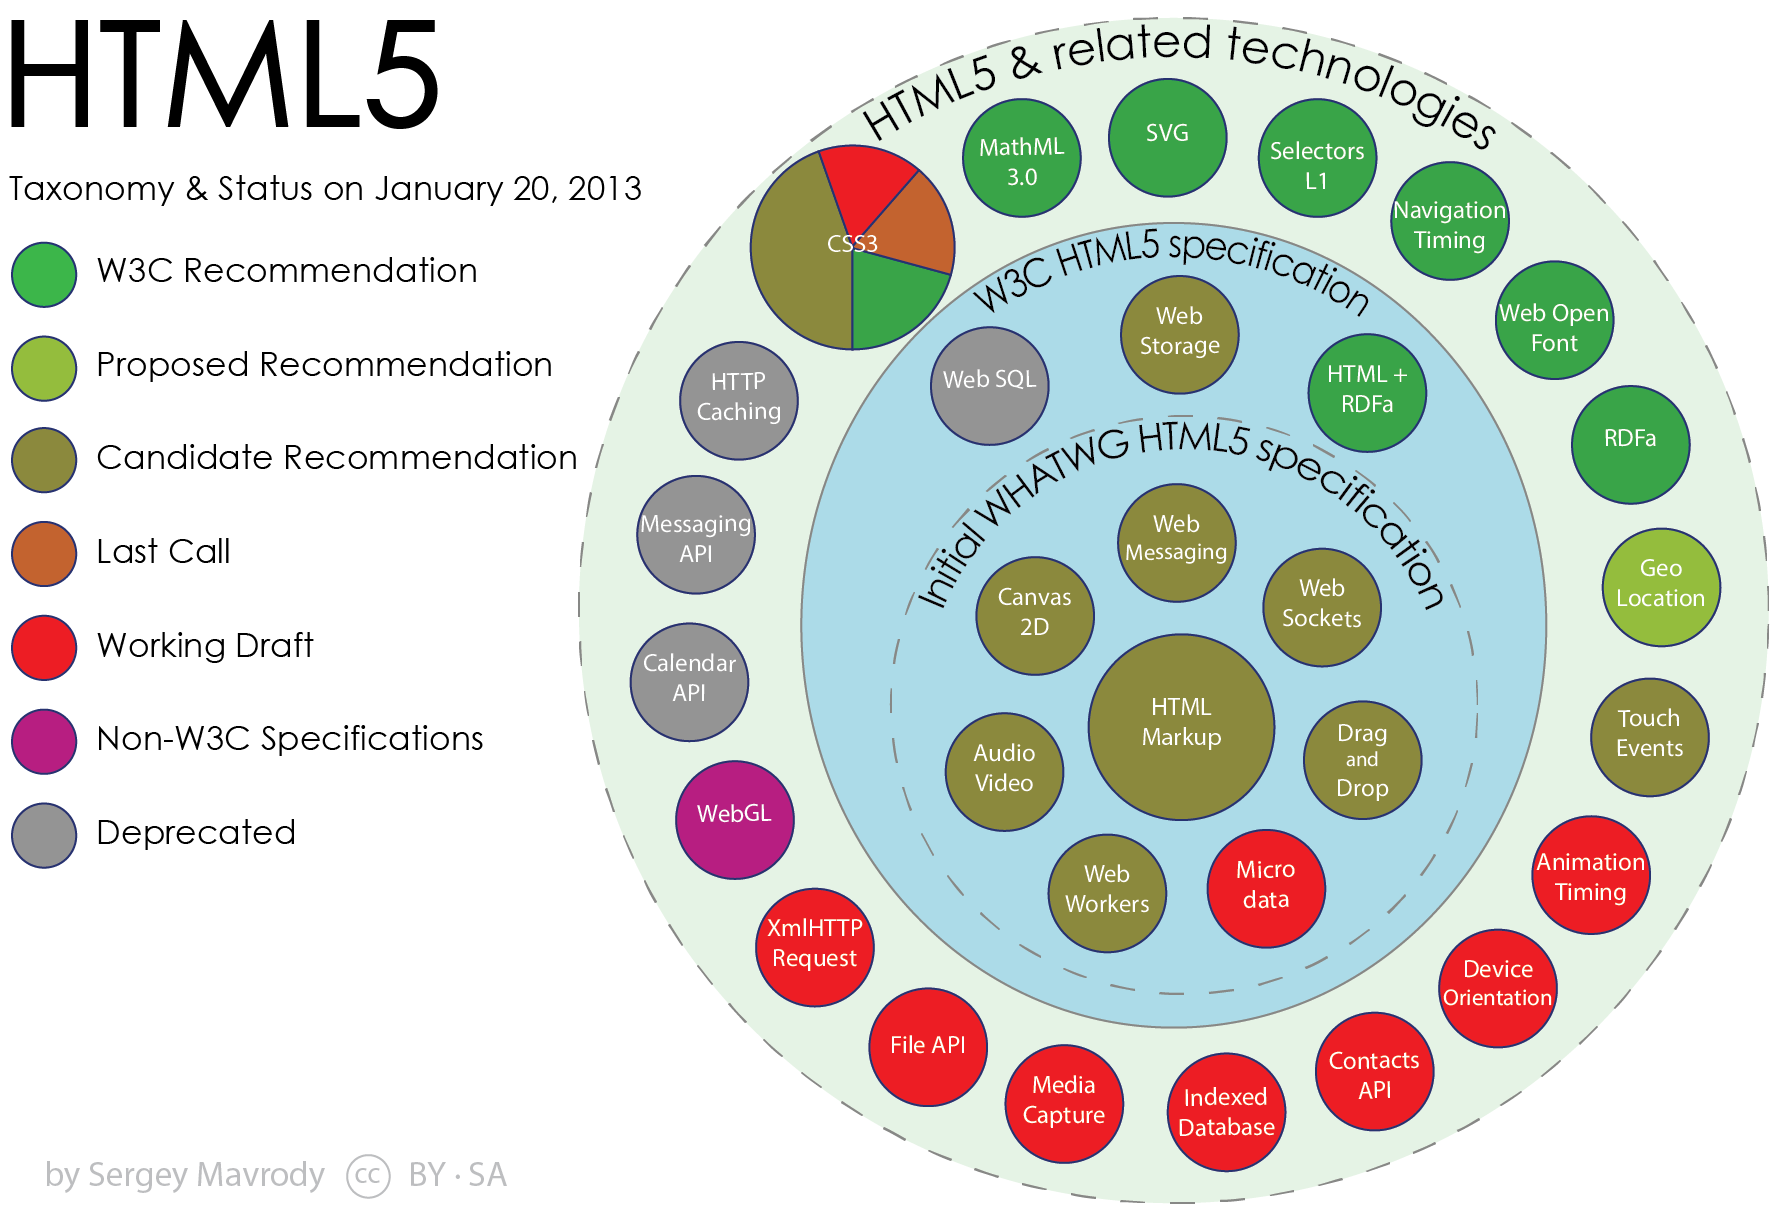
\includegraphics[scale=0.2]{HTML5-APIs-and-related-technologies.png}
\caption{HTML5 APIs and related technologies}
\label{HTML5-APIs-and-related-technologies}
\end{figure}

\chapter{Features}




\section{Markup}


HTML5 introduces elements and attributes that reflect typical usage on modern websites. Some of them are semantic replacements for common uses of generic block (<div>) and inline (<span>) elements, for example <nav> (website navigation block), <footer> (usually referring to bottom of web page or to last lines of HTML code), or <audio> and <video> instead of <object>. Some deprecated elements from HTML 4.01 have been dropped, including purely presentational elements such as <font> and <center>, whose effects have long been superseded by the more capable Cascading Style Sheets. There is also a renewed emphasis on the importance of DOM scripting (e.g., JavaScript) in Web behavior.

The HTML5 syntax is no longer based on SGML despite the similarity of its markup. It has, however, been designed to be backward compatible with common parsing of older versions of HTML. It comes with a new introductory line that looks like an SGML document type declaration, <!DOCTYPE html>, which triggers the standards-compliant rendering mode. As of 5 January 2009, HTML5 also includes Web Forms 2.0, a previously separate WHATWG specification.

通过制定如何处理所有 HTML 元素以及如何从错误中恢复的精确规则,HTML 5 改进了互操作性,并减少了开发成本。

HTML 5 中增加了嵌入音频、视频和图形的功能,客户端数据存储,以及交互式文档。

HTML 5 还包含了新的元素,比如:<nav>, <header>, <footer> 以及 <figure> 等等。


\subsection{HTML 5 Elements}


\begin{longtable}{|p{80pt}|p{260pt}|}
%head
\multicolumn{2}{r}{}
\tabularnewline\hline
标签	&描述
\endhead
%endhead

%firsthead
\caption{HTML 5 Elements}\\
\hline
标签	&描述
\endfirsthead
%endfirsthead

%foot
\multicolumn{2}{r}{}
\endfoot
%endfoot

%lastfoot
\endlastfoot
%endlastfoot
\hline
<!--...-->		&定义注释。\\
\hline
<!DOCTYPE> 	&定义文档类型。\\
\hline
<a>			&定义超链接。\\
\hline
<abbr>		&定义缩写。\\
\hline
<acronym>	&HTML 5 中不支持。定义首字母缩写。\\
\hline
<address>	&定义地址元素。\\
\hline
<applet>		&HTML 5 中不支持。定义 applet。\\
\hline
<area>		&定义图像映射中的区域。\\
\hline
<article>		&定义 article。\\
\hline
<aside>		&定义页面内容之外的内容。\\
\hline
<audio>		&定义声音内容。\\
\hline
<b>			&定义粗体文本。\\
\hline
<base>		&定义页面中所有链接的基准 URL。\\
\hline
<basefont>	&HTML 5 中不支持。需要使用 CSS 代替。\\
\hline
<bdi>		&定义文本的文本方向,使其脱离其周围文本的方向设置。\\
\hline
<bdo>		&定义文本显示的方向。\\
\hline
<big>		&HTML 5 中不支持。定义大号文本。\\
\hline
<blockquote>	&定义长的引用。\\
\hline
<body>		&定义 body 元素。\\
\hline
<br>			&插入换行符。\\
\hline
<button>		&定义按钮。\\
\hline
<canvas>		&定义图形。\\
\hline
<caption>		&定义表格标题。\\
\hline
<center>		&HTML 5 中不支持。定义居中的文本。\\
\hline
<cite>		&定义引用。\\
\hline
<code>		&定义计算机代码文本。\\
\hline
<col>		&定义表格列的属性。\\
\hline
<colgroup>	&定义表格列的分组。\\
\hline
<command>	&定义命令按钮。\\
\hline
<datalist>	&定义下拉列表。\\
\hline
<dd>		&定义定义的描述。\\
\hline
<del>		&定义删除文本。\\
\hline
<details>		&定义元素的细节。\\
\hline
<dfn>		&定义定义项目。\\
\hline
<dir>		&HTML 5 中不支持。定义目录列表。\\
\hline
<div>		&定义文档中的一个部分。\\
\hline
<dl>			&定义定义列表。\\
\hline
<dt>			&定义定义的项目。\\
\hline
<em>		&定义强调文本。\\
\hline
<embed>		&定义外部交互内容或插件。\\
\hline
<fieldset>	&定义 fieldset。\\
\hline
<figcaption>	&定义 figure 元素的标题。\\
\hline
<figure>		&定义媒介内容的分组,以及它们的标题。\\
\hline
<font>		&HTML 5 中不支持。\\
\hline
<footer>		&定义 section 或 page 的页脚。\\
\hline
<form>		&定义表单。\\
\hline
<frame>		&HTML 5 中不支持。定义子窗口(框架)。\\
\hline
<frameset>	&HTML 5 中不支持。定义框架的集。\\
\hline
<h1> to <h6>	&定义标题 1 到标题 6。\\
\hline
<head>		&定义关于文档的信息。\\
\hline
<header>		&定义 section 或 page 的页眉。\\
\hline
<hgroup>		&定义有关文档中的 section 的信息。\\
\hline
<hr>			&定义水平线。\\
\hline
<html>		&定义 html 文档。\\
\hline
<i>			&定义斜体文本。\\
\hline
<iframe>		&定义行内的子窗口(框架)。\\
\hline
<img>		&定义图像。\\
\hline
<input>		&定义输入域。\\
\hline
<ins>		&定义插入文本。\\
\hline
<keygen>		&定义生成密钥。\\
\hline
<isindex>		&HTML 5 中不支持。定义单行的输入域。\\
\hline
<kbd>		&定义键盘文本。\\
\hline
<label>		&定义表单控件的标注。\\
\hline
<legend>		&定义 fieldset 中的标题。\\
\hline
<li>			&定义列表的项目。\\
\hline
<link>		&定义资源引用。\\
\hline
<map>		&定义图像映射。\\
\hline
<mark>		&定义有记号的文本。\\
\hline
<menu>		&定义菜单列表。\\
\hline
<meta>		&定义元信息。\\
\hline
<meter>		&定义预定义范围内的度量。\\
\hline
<nav>		&定义导航链接。\\
\hline
<noframes>	&HTML 5 中不支持。定义 noframe 部分。\\
\hline
<noscript>	&定义 noscript 部分。\\
\hline
<object>		&定义嵌入对象。\\
\hline
<ol>			&定义有序列表。\\
\hline
<optgroup>	&定义选项组。\\
\hline
<option>		&定义下拉列表中的选项。\\
\hline
<output>		&定义输出的一些类型。\\
\hline
<p>			&定义段落。\\
\hline
<param>		&为对象定义参数。\\
\hline
<pre>		&定义预格式化文本。\\
\hline
<progress>	&定义任何类型的任务的进度。\\
\hline
<q>			&定义短的引用。\\
\hline
<rp>			&定义若浏览器不支持 ruby 元素显示的内容。\\
\hline
<rt>			&定义 ruby 注释的解释。\\
\hline
<ruby>		&定义 ruby 注释。\\
\hline
<s>			&HTML 5 中不支持。定义加删除线的文本。\\
\hline
<samp>		&定义样本计算机代码。\\
\hline
<script>		&定义脚本。\\
\hline
<section>		&定义 section。\\
\hline
<select>		&定义可选列表。\\
\hline
<small>		&将旁注 (side comments) 呈现为小型文本。\\
\hline
<source>		&定义媒介源。\\
\hline
<span>		&定义文档中的 section。\\
\hline
<strike>		&HTML 5 中不支持。定义加删除线的文本。\\
\hline
<strong>		&定义强调文本。\\
\hline
<style>		&定义样式定义。\\
\hline
<sub>		&定义下标文本。\\
\hline
<summary>	&定义 details 元素的标题。\\
\hline
<sup>		&定义上标文本。\\
\hline
<table>		&定义表格。\\
\hline
<tbody>		&定义表格的主体。\\
\hline
<td>			&定义表格单元。\\
\hline
<textarea>	&定义 textarea。\\
\hline
<tfoot>		&定义表格的脚注。\\
\hline
<th>			&定义表头。\\
\hline
<thead>		&定义表头。\\
\hline
<time>		&定义日期/时间。\\
\hline
<title>		&定义文档的标题。\\
\hline
<tr>			&定义表格行。\\
\hline
<track>		&定义用在媒体播放器中的文本轨道。\\
\hline
<tt>			&HTML 5 中不支持。定义打字机文本。\\
\hline
<u>			&HTML 5 中不支持。定义下划线文本。\\
\hline
<ul>			&定义无序列表。\\
\hline
<var>		&定义变量。\\
\hline
<video>		&定义视频。\\
\hline
<xmp>		&HTML 5 中不支持。定义预格式文本。\\
\hline
\end{longtable}

下面的表格列出了所有的HTML5/HTML 4.01/XHTML 元素,并定义了每个元素可以出现在哪种文档类型声明 (DTD) 中 。


\begin{longtable}{|l|l|l|l|l|l|}
%head
\multicolumn{6}{r}{...}
\tabularnewline\hline
\multirow{2}{80pt}{Tag}	&\multirow{2}{60pt}{HTML5} 	&\multicolumn{3}{c|}{HTML 4.01 / XHTML 1.0}		&\multirow{2}{50pt}{XHTML1.1} \\ \cline{3-5} 
						&							&Transitional		& Strict  	&  Frameset	 		& \multicolumn{1}{c|}{}
\endhead
%endhead

%firsthead
\caption{HTML5/HTML 4.01/XHTML 元素与DTD}\\
\hline
\multirow{2}{60pt}{Tag}	&\multirow{2}{60pt}{HTML5} 	&\multicolumn{3}{c|}{HTML 4.01 / XHTML 1.0}		&\multirow{2}{50pt}{XHTML1.1} \\ \cline{3-5} 
						&							&Transitional		& Strict  	&  Frameset	 		& \multicolumn{1}{c|}{}
\endfirsthead
%endfirsthead

%foot
\multicolumn{6}{r}{...}
\endfoot
%endfoot

\hline

%lastfoot
\endlastfoot
%endlastfoot
\hline
<a>				&Yes	&Yes			&Yes	&Yes				&Yes	\\
\hline
<abbr>			&Yes	&Yes			&Yes	&Yes				&Yes	\\
\hline
<acronym>		&No		&Yes			&Yes	&Yes				&Yes	\\
\hline
<address>		&Yes	&Yes			&Yes	&Yes				&Yes	\\
\hline
<applet>			&No		&Yes			&No		&Yes				&No		\\
\hline
<area>			&Yes	&Yes			&Yes	&Yes				&No		\\
\hline
<article>			&Yes	&No				&No		&No					&No		\\
\hline
<aside>			&Yes	&No				&No		&No					&No		\\
\hline
<audio>			&Yes	&No				&No		&No					&No		\\
\hline
<b>				&Yes	&Yes			&Yes	&Yes				&Yes	\\
\hline
<base>			&Yes	&Yes			&Yes	&Yes				&Yes	\\
\hline
<bdi>			&Yes	&No				&No		&No					&No		\\
\hline
<basefont>		&No		&Yes			&No		&Yes				&No		\\
\hline
<bdo>			&Yes	&Yes			&Yes	&Yes				&No		\\
\hline
<big>			&No		&Yes			&Yes	&Yes				&Yes	\\
\hline
<blockquote>		&Yes	&Yes			&Yes	&Yes				&Yes	\\
\hline
<body>			&Yes	&Yes			&Yes	&Yes				&Yes	\\
\hline
<br>				&Yes	&Yes			&Yes	&Yes				&Yes	\\
\hline
<button>			&Yes	&Yes			&Yes	&Yes				&Yes	\\
\hline
<canvas>			&Yes	&No				&No		&No					&No		\\
\hline
<caption>			&Yes	&Yes			&Yes	&Yes				&Yes	\\
\hline
<center>			&No		&Yes			&No		&Yes				&No		\\
\hline
<cite>			&Yes	&Yes			&Yes	&Yes				&Yes	\\
\hline
<code>			&Yes	&Yes			&Yes	&Yes				&Yes	\\
\hline
<col>			&Yes	&Yes			&Yes	&Yes				&No		\\
\hline
<colgroup>		&Yes	&Yes			&Yes	&Yes				&No		\\
\hline
<command>		&Yes	&No				&No		&No					&No		\\
\hline
<datalist>		&Yes	&No				&No		&No					&No		\\
\hline
<dd>			&Yes	&Yes			&Yes	&Yes				&Yes	\\
\hline
<del>			&Yes	&Yes			&Yes	&Yes				&No		\\
\hline
<details>			&Yes	&No				&No		&No					&No		\\
\hline
<dfn>			&Yes	&Yes			&Yes	&Yes				&Yes	\\
\hline
<dir>			&No		&Yes			&No		&Yes				&No		\\
\hline
<div>			&Yes	&Yes			&Yes	&Yes				&Yes	\\
\hline
<dl>				&Yes	&Yes			&Yes	&Yes				&Yes	\\
\hline
<dt>				&Yes	&Yes			&Yes	&Yes				&Yes	\\
\hline
<em>			&Yes	&Yes			&Yes	&Yes				&Yes	\\
\hline
<embed>			&Yes	&No				&No		&No					&No		\\
\hline
<fieldset>		&Yes	&Yes			&Yes	&Yes				&Yes	\\
\hline
<figcaption>		&Yes	&No				&No		&No					&No		\\
\hline
<figure>			&Yes	&No				&No		&No					&No		\\
\hline
<font>			&No		&Yes			&No		&Yes				&No		\\
\hline
<footer>			&Yes	&No				&No		&No					&No		\\
\hline
<form>			&Yes	&Yes			&Yes	&Yes				&Yes	\\
\hline
<frame>			&No		&No				&No		&Yes				&No		\\
\hline
<frameset>		&No		&No				&No		&Yes				&No		\\
\hline
<h1> to <h6>		&Yes	&Yes			&Yes	&Yes				&Yes	\\
\hline
<head>			&Yes	&Yes			&Yes	&Yes				&Yes	\\
\hline
<header>			&Yes	&No				&No		&No					&No		\\
\hline
<hgroup>			&Yes	&No				&No		&No					&No		\\
\hline
<hr>				&Yes	&Yes			&Yes	&Yes				&Yes	\\
\hline
<html>			&Yes	&Yes			&Yes	&Yes				&Yes	\\
\hline
<i>				&Yes	&Yes			&Yes	&Yes				&Yes	\\
\hline
<iframe>			&Yes	&Yes			&No		&Yes				&No		\\
\hline
<img>			&Yes	&Yes			&Yes	&Yes				&Yes	\\
\hline
<input>			&Yes	&Yes			&Yes	&Yes				&Yes	\\
\hline
<ins>			&Yes	&Yes			&Yes	&Yes				&No		\\
\hline
<isindex>			&No		&Yes			&No		&Yes				&No		\\
\hline
<kbd>			&Yes	&Yes			&Yes	&Yes				&Yes	\\
\hline
<keygen>			&Yes	&No				&No		&No					&No		\\
\hline
<label>			&Yes	&Yes			&Yes	&Yes				&Yes	\\
\hline
<legend>			&Yes	&Yes			&Yes	&Yes				&Yes	\\
\hline
<li>				&Yes	&Yes			&Yes	&Yes				&Yes	\\
\hline
<link>			&Yes	&Yes			&Yes	&Yes				&Yes	\\
\hline
<map>			&Yes	&Yes			&Yes	&Yes				&No		\\
\hline
<menu>			&Yes	&Yes			&No		&Yes				&No		\\
\hline
<meta>			&Yes	&Yes			&Yes	&Yes				&Yes	\\
\hline
<meter>			&Yes	&No				&No		&No					&No		\\
\hline
<nav>			&Yes	&No				&No		&No					&No		\\
\hline
<noframes>		&No		&Yes			&No		&Yes				&No		\\
\hline
<noscript>		&Yes	&Yes			&Yes	&Yes				&Yes	\\
\hline
<object>			&Yes	&Yes			&Yes	&Yes				&Yes	\\
\hline
<ol>				&Yes	&Yes			&Yes	&Yes				&Yes	\\
\hline
<optgroup>		&Yes	&Yes			&Yes	&Yes				&Yes	\\
\hline
<option>			&Yes	&Yes			&Yes	&Yes				&Yes	\\
\hline
<output>			&Yes	&No				&No		&No					&No		\\
\hline
<p>				&Yes	&Yes			&Yes	&Yes				&Yes	\\
\hline
<param>			&Yes	&Yes			&Yes	&Yes				&Yes	\\
\hline
<pre>			&Yes	&Yes			&Yes	&Yes				&Yes	\\
\hline
<progress>		&Yes	&No				&No		&No					&No		\\
\hline
<q>				&Yes	&Yes			&Yes	&Yes				&Yes	\\
\hline
<rp>				&Yes	&No				&No		&No					&No		\\
\hline
<rt>				&Yes	&No				&No		&No					&No		\\
\hline
<ruby>			&Yes	&No				&No		&No					&No		\\
\hline
<s>				&Yes	&Yes			&No		&Yes				&No		\\
\hline
<samp>			&Yes	&Yes			&Yes	&Yes				&Yes	\\
\hline
<script>			&Yes	&Yes			&Yes	&Yes				&Yes	\\
\hline
<section>			&Yes	&No				&No		&No					&No		\\
\hline
<select>			&Yes	&Yes			&Yes	&Yes				&Yes	\\
\hline
<small>			&Yes	&Yes			&Yes	&Yes				&Yes	\\
\hline
<source>			&Yes	&No				&No		&No					&No		\\
\hline
<span>			&Yes	&Yes			&Yes	&Yes				&Yes	\\
\hline
<strike>			&No		&Yes			&No		&Yes				&No		\\
\hline
<strong>			&Yes	&Yes			&Yes	&Yes				&Yes	\\
\hline
<style>			&Yes	&Yes			&Yes	&Yes				&Yes	\\
\hline
<sub>			&Yes	&Yes			&Yes	&Yes				&Yes	\\
\hline
<summary>		&Yes	&No				&No		&No					&No		\\
\hline
<sup>			&Yes	&Yes			&Yes	&Yes				&Yes	\\
\hline
<table>			&Yes	&Yes			&Yes	&Yes				&Yes	\\
\hline
<tbody>			&Yes	&Yes			&Yes	&Yes				&No		\\
\hline
<td>				&Yes	&Yes			&Yes	&Yes				&Yes	\\
\hline
<textarea>		&Yes	&Yes			&Yes	&Yes				&Yes	\\
\hline
<tfoot>			&Yes	&Yes			&Yes	&Yes				&No		\\
\hline
<th>				&Yes	&Yes			&Yes	&Yes				&Yes	\\
\hline
<thead>			&Yes	&Yes			&Yes	&Yes				&No		\\
\hline
<time>			&Yes	&No				&No		&No					&No		\\
\hline
<title>			&Yes	&Yes			&Yes	&Yes				&Yes	\\
\hline
<tr>				&Yes	&Yes			&Yes	&Yes				&Yes	\\
\hline
<track>			&Yes	&No				&No		&No					&No		\\
\hline
<tt>				&No		&Yes			&Yes	&Yes				&Yes	\\
\hline
<u>				&No		&Yes			&No		&Yes				&No		\\
\hline
<ul>				&Yes	&Yes			&Yes	&Yes				&Yes	\\
\hline
<var>			&Yes	&Yes			&Yes	&Yes				&Yes	\\
\hline
<video>			&Yes	&No				&No		&No					&No		\\
\hline
<wbr>			&Yes	&No				&No		&No					&No		\\
\hline
\end{longtable}



\subsection{HTML 5 Attributes}

所有 HTML 5 标签均支持下面列出的属性\footnote{注释:HTML 4.01 不再支持 accesskey 属性:},仅有少数例外。

\begin{longtable}{|p{70pt}|p{70pt}|p{230pt}|}
%head
\multicolumn{3}{r}{}
\tabularnewline\hline
属性	&值	&描述
\endhead
%endhead

%firsthead
\caption{HTML 5 Attributes}\\
\hline
属性	&值	&描述
\endfirsthead
%endfirsthead

%foot
\multicolumn{3}{r}{}
\endfoot
%endfoot

%lastfoot
\endlastfoot
%endlastfoot
\hline
accesskey	&character			&规定访问元素的键盘快捷键\\
\hline
class		&classname			&规定元素的类名(用于规定样式表中的类)。\\
\hline
contenteditable&true \newline false	&规定是否允许用户编辑内容。\\
\hline
contextmenu	&menu\_id			&规定元素的上下文菜单。\\
\hline
data-yourvalue&value				&创作者定义的属性。\newline HTML 文档的创作者可以定义他们自己的属性。\newline 必须以``data-" 开头。\\
\hline
dir			& ltr \newline rtl		&规定元素中内容的文本方向。\\
\hline
draggable	& true\newline false \newline auto &规定是否允许用户拖动元素。\\
\hline
hidden		&hidden				&规定该元素是无关的。被隐藏的元素不会显示。\\
\hline
id			&id					&规定元素的唯一 ID。\\
\hline
item			&empty \newline url 	&用于组合元素。\\
\hline
itemprop		&url \newline group value&用于组合项目。\\
\hline
lang			&language\_code		&规定元素中内容的语言代码。\\
\hline
spellcheck	&true\newline false	&规定是否必须对元素进行拼写或语法检查。\\
\hline
style		&style\_definition		&规定元素的行内样式。\\
\hline
subject		&id					&规定元素对应的项目。\\
\hline
tabindex		&number				&规定元素的 tab 键控制次序。\\
\hline
title			&text				&规定有关元素的额外信息。\\
\hline

\end{longtable}


\subsection{HTML 5 Events}

HTML 4 增加了通过事件触发浏览器中行为的能力,比如当用户点击某个元素时启动一段 JavaScript。

下面的表格列出了可插入 HTML 5 元素中以定义事件行为的标准事件属性。


\begin{compactitem}
\item Window 事件属性 - Window Event Attributes
\item 表单事件 - Form Events
\item 键盘事件 - Keybord Events
\item 鼠标事件 - Mouse Events
\item 媒介事件 - Media Events
\end{compactitem}


\subsubsection{HTML 5 Window Event Attributes}

window 对象触发的事件,适用于 <body> 标签。

\CTEXnoindent
\begin{longtable}{|p{90pt}|p{40pt}|p{240pt}|}
%head
\multicolumn{3}{r}{}
\tabularnewline\hline
属性	&值	&描述
\endhead
%endhead

%firsthead
\caption{HTML 5 Window Event Attributes}\\
\hline
属性	&值	&描述
\endfirsthead
%endfirsthead

%foot
\multicolumn{3}{r}{}
\endfoot
%endfoot

%lastfoot
\endlastfoot
%endlastfoot
\hline

onafterprint		&script	&在打印文档之后运行脚本\\
\hline
onbeforeprint		&script	&在文档打印之前运行脚本\\
\hline
onbeforeonload	&script	&在文档加载之前运行脚本\\
\hline
onblur			&script	&当窗口失去焦点时运行脚本\\
\hline
onerror			&script	&当错误发生时运行脚本\\
\hline
onfocus			&script	&当窗口获得焦点时运行脚本\\
\hline
onhaschange		&script	&当文档改变时运行脚本\\
\hline
onload			&script	&当文档加载时运行脚本\\
\hline
onmessage		&script	&当触发消息时运行脚本\\
\hline
onoffline			&script	&当文档离线时运行脚本\\
\hline
ononline			&script	&当文档上线时运行脚本\\
\hline
onpagehide		&script	&当窗口隐藏时运行脚本\\
\hline
onpageshow		&script	&当窗口可见时运行脚本\\
\hline
onpopstate		&script	&当窗口历史记录改变时运行脚本\\
\hline
onredo			&script	&当文档执行再执行操作(redo)时运行脚本\\
\hline
onresize			&script	&当调整窗口大小时运行脚本\\
\hline
onstorage		&script	&当文档加载加载时运行脚本\\
\hline
onundo			&script	&当 Web Storage 区域更新时(存储空间中的数据发生变化时)\\
\hline
onunload			&script	&当用户离开文档时运行脚本\\
\hline
\end{longtable}


\CTEXindent


\subsubsection{HTML 5 Form Events}


由 HTML 表单内部的动作触发的事件,适用于所有 HTML 5 元素,不过最常用于表单元素中。

\begin{longtable}{|p{90pt}|p{40pt}|p{240pt}|}
%head
\multicolumn{3}{r}{}
\tabularnewline\hline
属性	&值	&描述
\endhead
%endhead

%firsthead
\caption{HTML 5 Form Events}\\
\hline
属性	&值	&描述
\endfirsthead
%endfirsthead

%foot
\multicolumn{3}{r}{}
\endfoot
%endfoot

%lastfoot
\endlastfoot
%endlastfoot
\hline
onblur			&script	&当元素失去焦点时运行脚本\\
\hline
onchange			&script	&当元素改变时运行脚本\\
\hline
oncontextmenu	&script	&当触发上下文菜单时运行脚本\\
\hline
onfocus			&script	&当元素获得焦点时运行脚本\\
\hline
onformchange		&script	&当表单改变时运行脚本\\
\hline
onforminput		&script	&当表单获得用户输入时运行脚本\\
\hline
oninput			&script	&当元素获得用户输入时运行脚本\\
\hline
oninvalid			&script	&当元素无效时运行脚本\\
\hline
onreset			&script	&当表单重置时运行脚本。HTML 5 不支持。\\
\hline
onselect			&script	&当选取元素时运行脚本\\
\hline
onsubmit			&script	&当提交表单时运行脚本\\
\hline
\end{longtable}


\subsubsection{HTML 5 Keyboard Events}

由键盘触发的事件,适用于所有 HTML 5 元素。

\begin{longtable}{|p{90pt}|p{40pt}|p{240pt}|}
%head
\multicolumn{3}{r}{}
\tabularnewline\hline
属性	&值	&描述
\endhead
%endhead

%firsthead
\caption{HTML 5 Keyboard Events}\\
\hline
属性	&值	&描述
\endfirsthead
%endfirsthead

%foot
\multicolumn{3}{r}{}
\endfoot
%endfoot

%lastfoot
\endlastfoot
%endlastfoot
\hline
onkeydown	&script	&当按下按键时运行脚本\\
\hline
onkeypress	&script	&当按下并松开按键时运行脚本\\
\hline
onkeyup		&script	&当松开按键时运行脚本\\
\hline

\end{longtable}


\subsubsection{HTML 5 Mouse Events}

由鼠标或相似的用户动作触发的事件,适用于所有 HTML 5 元素。

\begin{longtable}{|p{90pt}|p{40pt}|p{240pt}|}
%head
\multicolumn{3}{r}{}
\tabularnewline\hline
属性	&值	&描述
\endhead
%endhead

%firsthead
\caption{HTML 5 Mouse Events}\\
\hline
属性	&值	&描述
\endfirsthead
%endfirsthead

%foot
\multicolumn{3}{r}{}
\endfoot
%endfoot

%lastfoot
\endlastfoot
%endlastfoot
\hline
onclick		&script	&当单击鼠标时运行脚本\\
\hline
ondblclick	&script	&当双击鼠标时运行脚本\\
\hline
ondrag		&script	&当拖动元素时运行脚本\\
\hline
ondragend	&script	&当拖动操作结束时运行脚本\\
\hline
ondragenter	&script	&当元素被拖动至有效的拖放目标时运行脚本\\
\hline
ondragleave	&script	&当元素离开有效拖放目标时运行脚本\\
\hline
ondragover	&script	&当元素被拖动至有效拖放目标上方时运行脚本\\
\hline
ondragstart	&script	&当拖动操作开始时运行脚本\\
\hline
ondrop		&script	&当被拖动元素正在被拖放时运行脚本\\
\hline
onmousedown	&script	&当按下鼠标按钮时运行脚本\\
\hline
onmousemove	&script	&当鼠标指针移动时运行脚本\\
\hline
onmouseout	&script	&当鼠标指针移出元素时运行脚本\\
\hline
onmouseover	&script	&当鼠标指针移至元素之上时运行脚本\\
\hline
onmouseup	&script	&当松开鼠标按钮时运行脚本\\
\hline
onmousewheel&script	&当转动鼠标滚轮时运行脚本\\
\hline
onscroll		&script	&当滚动元素滚动元素的滚动条时运行脚本\\
\hline
\end{longtable}

\subsubsection{HTML 5 Media Events}

由视频、图像以及音频等媒介触发的事件,适用于所有 HTML 5 元素,不过在媒介元素(诸如 audio、embed、img、object 以及 video)中最常用。


\begin{longtable}{|p{90pt}|p{40pt}|p{240pt}|}
%head
\multicolumn{3}{r}{}
\tabularnewline\hline
属性	&值	&描述
\endhead
%endhead

%firsthead
\caption{HTML 5 Media Events}\\
\hline
属性	&值	&描述
\endfirsthead
%endfirsthead

%foot
\multicolumn{3}{r}{}
\endfoot
%endfoot

%lastfoot
\endlastfoot
%endlastfoot
\hline
onabort			&script	&当发生中止事件时运行脚本\\
\hline
oncanplay		&script	&当媒介能够开始播放但可能因缓冲而需要停止时运行脚本\\
\hline
oncanplaythrough	&script	&当媒介能够无需因缓冲而停止即可播放至结尾时运行脚本\\
\hline
ondurationchange	&script	&当媒介长度改变时运行脚本\\
\hline
onemptied		&script	&当媒介资源元素突然为空时(网络错误、加载错误等)运行脚本\\
\hline
onended			&script	&当媒介已抵达结尾时运行脚本\\
\hline
onerror			&script	&当在元素加载期间发生错误时运行脚本\\
\hline
onloadeddata		&script	&当加载媒介数据时运行脚本\\
\hline
onloadedmetadata	&script	&当媒介元素的持续时间以及其他媒介数据已加载时运行脚本\\
\hline
onloadstart		&script	&当浏览器开始加载媒介数据时运行脚本\\
\hline
onpause			&script	&当媒介数据暂停时运行脚本\\
\hline
onplay			&script	&当媒介数据将要开始播放时运行脚本\\
\hline
onplaying			&script	&当媒介数据已开始播放时运行脚本\\
\hline
onprogress		&script	&当浏览器正在取媒介数据时运行脚本\\
\hline
onratechange		&script	&当媒介数据的播放速率改变时运行脚本\\
\hline
onreadystatechange&script	&当就绪状态(ready-state)改变时运行脚本\\
\hline
onseeked			&script	&当媒介元素的定位属性(seeking attribute)不再为真且定位已结束时运行脚本\\
\hline
onseeking		&script	&当媒介元素的定位属性为真且定位已开始时运行脚本\\
\hline
onstalled			&script	&当取回媒介数据过程中(延迟)存在错误时运行脚本\\
\hline
onsuspend		&script	&当浏览器已在取媒介数据但在取回整个媒介文件之前停止时运行脚本\\
\hline
ontimeupdate		&script	&当媒介改变其播放位置时运行脚本\\
\hline
onvolumechange	&script	&当媒介改变音量亦或当音量被设置为静音时运行脚本\\
\hline
onwaiting			&script	&当媒介已停止播放但打算继续播放时运行脚本\\
\hline
\end{longtable}


\section{HTML 5 Input}

HTML5 拥有多个新的表单输入类型,这些新特性提供了更好的输入控制和验证。


\begin{compactitem}
\item email
\item url
\item number
\item range
\item Date pickers (date, month, week, time, datetime, datetime-local)
\item search
\item color
\end{compactitem}

\begin{longtable}{|p{80pt}|p{50pt}|p{50pt}|p{50pt}|p{50pt}|p{50pt}|}
%head
\multicolumn{6}{r}{}
\tabularnewline\hline
Input type	&IE	&Firefox	&Opera	&Chrome	&Safari
\endhead
%endhead

%firsthead
\caption{HTML 5 Input 类型}\\
\hline
Input type	&IE	&Firefox	&Opera	&Chrome	&Safari
\endfirsthead
%endfirsthead

%foot
\multicolumn{6}{r}{}
\endfoot
%endfoot

%lastfoot
\endlastfoot
%endlastfoot
\hline
email	&No		&4.0	&9.0	&10.0	&No\\
\hline
url		&No		&4.0	&9.0	&10.0	&No\\
\hline
number	&No		&No		&9.0	&7.0	&No\\
\hline
range	&No		&No		&9.0	&4.0	&4.0\\
\hline
Date pickers&	No	&No		&9.0	&10.0	&No\\
\hline
search	&No		&4.0	&11.0	&10.0	&No\\
\hline
color	&No		&No		&11.0	&No		&No\\
\hline
\end{longtable}



Opera 对新的输入类型的支持最好。不过即使在其他浏览器中不被支持,仍然可以显示为常规的文本域。

\subsection{email}

email 类型用于应该包含 e-mail 地址的输入域。在提交表单时,会自动验证 email 域的值。

\begin{lstlisting}[language=HTML]
E-mail: <input type="email" name="user_email" />
\end{lstlisting}

iPhone 中的 Safari 浏览器支持 email 输入类型,并通过改变触摸屏键盘来配合它(添加 @ 和 .com 选项)。


\subsection{url}

url 类型用于应该包含 URL 地址的输入域。在提交表单时,会自动验证 url 域的值。

\begin{lstlisting}[language=HTML]
Homepage: <input type="url" name="user_url" />
\end{lstlisting}

iPhone 中的 Safari 浏览器支持 url 输入类型,并通过改变触摸屏键盘来配合它(添加 .com 选项)。


\subsection{number}

number 类型用于应该包含数值的输入域。另外,还可以设定对所接受的数字的限定:

\begin{lstlisting}[language=HTML]
Points: <input type="number" name="points" min="1" max="10" />
\end{lstlisting}

使用下面的属性来规定对数字类型的限定:

\begin{longtable}{|p{80pt}|p{50pt}|p{200pt}|}
%head
\multicolumn{3}{r}{}
\tabularnewline\hline
属性	&值	&描述
\endhead
%endhead

%firsthead
\caption{HTML 5 数字类型的限定}\\
\hline
属性	&值	&描述
\endfirsthead
%endfirsthead

%foot
\multicolumn{3}{r}{}
\endfoot
%endfoot

%lastfoot
\endlastfoot
%endlastfoot
\hline
max	&number	&规定允许的最大值\\
\hline
min	&number	&规定允许的最小值\\
\hline
step	&number	&规定合法的数字间隔(如果 step="3",则合法的数是 -3,0,3,6 等)\\
\hline
value&number	&规定默认值\\
\hline

\end{longtable}

iPhone 中的 Safari 浏览器支持 number 输入类型,并通过改变触摸屏键盘来配合它(显示数字)。



\subsection{range}

range 类型用于应该包含一定范围内数字值的输入域。range 类型显示为滑动条。

另外,也能够设定对所接受的数字的限定:

\begin{lstlisting}[language=HTML]
<input type="range" name="points" min="1" max="10" />
\end{lstlisting}

使用下面的属性来规定对数字类型的限定:


\begin{longtable}{|p{80pt}|p{50pt}|p{200pt}|}
%head
\multicolumn{3}{r}{}
\tabularnewline\hline
属性	&值	&描述
\endhead
%endhead

%firsthead
\caption{HTML 5 数字类型的限定}\\
\hline
属性	&值	&描述
\endfirsthead
%endfirsthead

%foot
\multicolumn{3}{r}{}
\endfoot
%endfoot

%lastfoot
\endlastfoot
%endlastfoot
\hline
max	&number	&规定允许的最大值\\
\hline
min	&number	&规定允许的最小值\\
\hline
step	&number	&规定合法的数字间隔(如果 step="3",则合法的数是 -3,0,3,6 等)\\
\hline
value&number	&规定默认值\\
\hline

\end{longtable}





\subsection{Date Pickers}


HTML5 拥有多个可供选取日期和时间的新输入类型:


\begin{compactitem}
\item date - 选取日、月、年
\item month - 选取月、年
\item week - 选取周和年
\item time - 选取时间(小时和分钟)
\item datetime - 选取时间、日、月、年(UTC 时间)
\item datetime-local - 选取时间、日、月、年(本地时间)
\end{compactitem}

下面的例子允许用户从日历中选取一个日期:

\begin{lstlisting}[language=HTML]
Date: <input type="date" name="user_date" />
\end{lstlisting}

\subsection{search}


search 类型用于搜索域,比如站点搜索或 Google 搜索。search 域显示为常规的文本域。




\section{HTML 5 Form}


HTML 5新的表单元素包括:

\begin{compactitem}
\item datalist
\item keygen
\item output
\end{compactitem}



HTML5 拥有若干涉及表单的元素和属性。


\begin{longtable}{|p{80pt}|p{50pt}|p{50pt}|p{50pt}|p{50pt}|p{50pt}|}
%head
\multicolumn{6}{r}{}
\tabularnewline\hline
Input type	&IE	&Firefox	&Opera	&Chrome	&Safari
\endhead
%endhead

%firsthead
\caption{HTML 5 Form 类型}\\
\hline
Input type	&IE	&Firefox	&Opera	&Chrome	&Safari
\endfirsthead
%endfirsthead

%foot
\multicolumn{6}{r}{}
\endfoot
%endfoot

%lastfoot
\endlastfoot
%endlastfoot
\hline
datalist	&No		&No		&9.5	&No		&No\\
\hline
keygen	&No		&No		&10.5	&3.0	&No\\
\hline
output	&No		&No		&9.5	&No		&No\\
\hline

\end{longtable}



\subsection{datalist}


datalist 元素规定输入域的选项列表。

列表是通过 datalist 内的 option 元素\footnote{提示:option 元素永远都要设置 value 属性。}创建的。

如需把 datalist 绑定到输入域,需要用输入域的 list 属性引用 datalist 的 id:

\begin{lstlisting}[language=HTML]
Webpage: <input type="url" list="url_list" name="link" />
<datalist id="url_list">
<option label="W3School" value="http://www.W3School.com.cn" />
<option label="Google" value="http://www.google.com" />
<option label="Microsoft" value="http://www.microsoft.com" />
</datalist>
\end{lstlisting}






\subsection{keygen}

keygen 元素的作用是提供一种验证用户的可靠方法\footnote{目前,浏览器对此元素的糟糕的支持度不足以使其成为一种有用的安全标准。}。

keygen 元素是密钥对生成器(key-pair generator)。当提交表单时,会生成两个键,一个是私钥,一个公钥。

私钥(private key)存储于客户端,公钥(public key)则被发送到服务器。公钥可用于之后验证用户的客户端证书(client certificate)。

\begin{lstlisting}[language=HTML]
<form action="demo_form.asp" method="get">
Username: <input type="text" name="usr_name" />
Encryption: <keygen name="security" />
<input type="submit" />
</form>
\end{lstlisting}


\subsection{output}


output 元素用于不同类型的输出,比如计算或脚本输出:

\begin{lstlisting}[language=HTML]
<output id="result" onforminput="resCalc()"></output>
\end{lstlisting}


\begin{longtable}{|p{80pt}|p{50pt}|p{50pt}|p{50pt}|p{50pt}|p{50pt}|}
%head
\multicolumn{6}{r}{}
\tabularnewline\hline
Input type	&IE	&Firefox	&Opera	&Chrome	&Safari
\endhead
%endhead

%firsthead
\caption{HTML 5 表单属性}\\
\hline
Input type	&IE	&Firefox	&Opera	&Chrome	&Safari
\endfirsthead
%endfirsthead

%foot
\multicolumn{6}{r}{}
\endfoot
%endfoot

%lastfoot
\endlastfoot
%endlastfoot
\hline
autocomplete	&8.0	&3.5	&9.5	&3.0	&4.0\\
\hline
autofocus	&No		&No		&10.0	&3.0	&4.0\\
\hline
form			&No		&No		&9.5	&No		&No\\
\hline
form overrides	&No		&No		&10.5	&No		&No\\
\hline
height and width&	8.0	&3.5	&9.5	&3.0	&4.0\\
\hline
list			&No		&No		&9.5	&No		&No\\
\hline
min, max and step&	No	&No		&9.5	&3.0	&No\\
\hline
multiple		&No		&3.5	&No		&3.0	&4.0\\
\hline
novalidate	&No		&No		&No		&No		&No\\
\hline
pattern		&No		&No		&9.5	&3.0	&No\\
\hline
placeholder	&No		&No		&No		&3.0	&3.0\\
\hline
required		&No		&No		&9.5	&3.0	&No\\
\hline

\end{longtable}



\subsection{autocomplete}

autocomplete\footnote{注释:autocomplete 适用于 <form> 标签,以及以下类型的 <input> 标签:text, search, url, telephone, email, password, datepickers, range 以及 color。} 属性规定 form 或 input 域应该拥有自动完成功能。

当用户在自动完成域中开始输入时,浏览器应该在该域中显示填写的选项:

\begin{lstlisting}[language=HTML]
<form action="demo_form.asp" method="get" autocomplete="on">
First name: <input type="text" name="fname" /><br />
Last name: <input type="text" name="lname" /><br />
E-mail: <input type="email" name="email" autocomplete="off" /><br />
<input type="submit" />
</form>
\end{lstlisting}

注释:在某些浏览器中,可能需要启用自动完成功能,以使该属性生效。


\subsection{autofocus}


autofocus\footnote{注释:autofocus 属性适用于所有 <input> 标签的类型。} 属性规定在页面加载时,域自动地获得焦点。

\begin{lstlisting}[language=HTML]
User name: <input type="text" name="user_name"  autofocus="autofocus" />
\end{lstlisting}



\subsection{form}

form\footnote{注释:form 属性适用于所有 <input> 标签的类型。} 属性规定输入域所属的一个或多个表单。

form 属性必须引用所属表单的 id:


\begin{lstlisting}[language=HTML]
<form action="demo_form.asp" method="get" id="user_form">
First name:<input type="text" name="fname" />
<input type="submit" />
</form>
Last name: <input type="text" name="lname" form="user_form" />
\end{lstlisting}

注释:如需引用一个以上的表单,需要使用空格分隔的列表。

\subsection{override}

表单重写属性(form override attributes)\footnote{注释:表单重写属性适用于以下类型的 <input> 标签:submit 和 image。}允许开发者重写 form 元素的某些属性设定。


表单重写属性有:

\begin{compactitem}
\item formaction - 重写表单的 action 属性
\item formenctype - 重写表单的 enctype 属性
\item formmethod - 重写表单的 method 属性
\item formnovalidate - 重写表单的 novalidate 属性
\item formtarget - 重写表单的 target 属性
\end{compactitem}


\begin{lstlisting}[language=HTML]
<form action="demo_form.asp" method="get" id="user_form">
E-mail: <input type="email" name="userid" /><br />
<input type="submit" value="Submit" />
<br />
<input type="submit" formaction="demo_admin.asp" value="Submit as admin" />
<br />
<input type="submit" formnovalidate="true" value="Submit without validation" />
<br />
</form>
\end{lstlisting}

注释:这些属性对于创建不同的提交按钮很有帮助。


\subsection{height \& width}

height\footnote{注释:height 和 width 属性只适用于 image 类型的 <input> 标签。} 和 width\footnote{注释:height 和 width 属性只适用于 image 类型的 <input> 标签。} 属性规定用于 image 类型的 input 标签的图像高度和宽度。

\begin{lstlisting}[language=HTML]
<input type="image" src="img_submit.gif" width="99" height="99" />
\end{lstlisting}




\subsection{list}

list\footnote{注释:list 属性适用于以下类型的 <input> 标签:text, search, url, telephone, email, date pickers, number, range 以及 color。} 属性规定输入域的 datalist,datalist 是输入域的选项列表。


\begin{lstlisting}[language=HTML]
Webpage: <input type="url" list="url_list" name="link" />
<datalist id="url_list">
<option label="W3Schools" value="http://www.w3school.com.cn" />
<option label="Google" value="http://www.google.com" />
<option label="Microsoft" value="http://www.microsoft.com" />
</datalist>
\end{lstlisting}



\subsection{min, max, step}

min\footnote{注释:min、max 和 step 属性适用于以下类型的 <input> 标签:date pickers、number 以及 range。}、max\footnote{注释:min、max 和 step 属性适用于以下类型的 <input> 标签:date pickers、number 以及 range。} 和 step\footnote{注释:min、max 和 step 属性适用于以下类型的 <input> 标签:date pickers、number 以及 range。} 属性用于为包含数字或日期的 input 类型规定限定(约束),其中:

\begin{compactitem}
\item max 属性规定输入域所允许的最大值。
\item min 属性规定输入域所允许的最小值。
\item step 属性为输入域规定合法的数字间隔(如果 step="3",则合法的数是 -3,0,3,6 等)。
\end{compactitem}

下面的例子显示一个数字域,该域接受介于 0 到 10 之间的值,且步进为 3(即合法的值为 0、3、6 和 9):

\begin{lstlisting}[language=HTML]
Points: <input type="number" name="points" min="0" max="10" step="3" />
\end{lstlisting}


\subsection{multiple}

multiple\footnote{注释:multiple 属性适用于以下类型的 <input> 标签:email 和 file。} 属性规定输入域中可选择多个值。


\begin{lstlisting}[language=HTML]
Select images: <input type="file" name="img" multiple="multiple" />
\end{lstlisting}



\subsection{novalidate}


novalidate\footnote{注释:novalidate 属性适用于 <form> 以及以下类型的 <input> 标签:text, search, url, telephone, email, password, date pickers, range 以及 color.} 属性规定在提交表单时不应该验证 form 或 input 域。

\begin{lstlisting}[language=HTML]
<form action="demo_form.asp" method="get" novalidate="true">
E-mail: <input type="email" name="user_email" />
<input type="submit" />
</form>
\end{lstlisting}


\subsection{pattern}

pattern\footnote{注释:pattern 属性适用于以下类型的 <input> 标签:text, search, url, telephone, email 以及 password。} 属性规定用于验证 input 域的模式(pattern),模式(pattern) 是正则表达式。


下面的例子显示了一个只能包含三个字母的文本域(不含数字及特殊字符):

\begin{lstlisting}[language=HTML]
Country code: <input type="text" name="country_code"
pattern="[A-z]{3}" title="Three letter country code" />
\end{lstlisting}



\subsection{placeholder}

placeholder\footnote{注释:placeholder 属性适用于以下类型的 <input> 标签:text, search, url, telephone, email 以及 password。} 属性提供一种提示(hint),描述输入域所期待的值。

提示(hint)会在输入域为空时显示出现,会在输入域获得焦点时消失:

\begin{lstlisting}[language=HTML]
<input type="search" name="user_search"  placeholder="Search" />
\end{lstlisting}


\subsection{required}

required\footnote{注释:required 属性适用于以下类型的 <input> 标签:text, search, url, telephone, email, password, date pickers, number, checkbox, radio 以及 file。} 属性规定必须在提交之前填写输入域(不能为空)。


\begin{lstlisting}[language=HTML]
Name: <input type="text" name="usr_name" required="required" />
\end{lstlisting}




\section{APIs}


In addition to specifying markup, HTML5 specifies scripting application programming interfaces (APIs) that can be used with JavaScript. Existing document object model (DOM) interfaces are extended and de facto features documented. There are also new APIs, such as:

\begin{compactitem}
\item The canvas element for immediate mode 2D drawing. 
\item Timed media playback
\item Offline Web Applications
\item Document editing
\item Drag-and-drop
\item Cross-document messaging
\item Browser history management
\item MIME type and protocol handler registration
\item Microdata
\item Web Storage, a key-value pair storage framework that provides behaviour similar to cookies but with larger storage capacity and improved API
\end{compactitem}


Not all of the above technologies are included in the W3C HTML5 specification, though they are in the WHATWG HTML specification. Some related technologies, which are not part of either the W3C HTML5 or the WHATWG HTML specification, are as follows. The W3C publishes specifications for these separately:

\begin{compactitem}
\item Geolocation
\item Web SQL Database, a local SQL Database (no longer maintained).
\item The Indexed Database API, an indexed hierarchical key-value store (formerly WebSimpleDB).
\item HTML5 File API, handles file uploads and file manipulation.
\item Directories and System, an API intended to satisfy client-side-storage use cases not well served by databases.
\item File Writer, an API for writing to files from web applications.
\item Web Audio API, a high-level JavaScript API for processing and synthesizing audio in web applications.
\end{compactitem}

HTML5 alone cannot provide animation within web pages. Either JavaScript or CSS3 is necessary for animating HTML elements. Animation is also possible using JavaScript and HTML 4, and within SVG elements through SMIL, although browser support of the latter remains uneven as of 2011.

\section{2D drawing}

HTML5 的 canvas 元素使用 JavaScript 在网页上绘制图像,canvas 拥有多种绘制路径、矩形、圆形、字符以及添加图像的方法。

画布是一个矩形区域,开发者可以控制其每一像素。不过,<canvas> 元素本身并没有绘制能力(它仅仅是图形的容器),开发者必须使用脚本来完成实际的绘图任务\footnote{Internet Explorer 9、Firefox、Opera、Chrome 以及 Safari 支持 <canvas> 及其属性和方法。Internet Explorer 8 以及更早的版本不支持 <canvas> 元素。}。

向 HTML5 页面添加 canvas 元素时,要规定元素的 id、宽度和高度:

\begin{lstlisting}[language=HTML]
<canvas id="myCanvas" width="200" height="100"></canvas>
\end{lstlisting}


\subsection{rectangle}


canvas 元素本身是没有绘图能力的,所有的绘制工作必须在 JavaScript 内部完成:

\begin{lstlisting}[language=JavaScript]
<script type="text/javascript">
  var c=document.getElementById("myCanvas");
  var cxt=c.getContext("2d");
  cxt.fillStyle="#FF0000";
  cxt.fillRect(0,0,150,75);
</script>
\end{lstlisting}

getContext() 方法可返回一个对象,该对象提供了用于在画布上绘图的方法和属性。


JavaScript 使用 id 来寻找 canvas 元素:

\begin{lstlisting}[language=JavaScript]
var c=document.getElementById("myCanvas");
\end{lstlisting}

然后,创建 context 对象:

\begin{lstlisting}[language=JavaScript]
var cxt=c.getContext("2d"); 
\end{lstlisting}

getContext(``2d") 对象是内建的 HTML5 对象,拥有多种绘制路径、矩形、圆形、字符以及添加图像的方法。

下面的两行代码绘制一个红色的矩形:

\begin{lstlisting}[language=JavaScript]
cxt.fillStyle="#FF0000";
cxt.fillRect(0,0,150,75); 
\end{lstlisting}

fillStyle 方法将其染成红色,fillRect 方法规定了形状、位置和尺寸。

这里的 fillRect 方法拥有参数 (0,0,150,75),意义是在画布上绘制 150$\times$75 的矩形,从左上角开始 (0,0)。

如下图所示,画布的 X 和 Y 坐标用于在画布上对绘画进行定位。

\begin{figure}[!h]
\centering
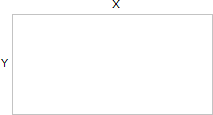
\includegraphics[scale=0.5]{html5_canvas_coordinates.png}
\caption{画布的 X 和 Y 坐标}
\label{html5_canvas_coordinates}
\end{figure}

\subsection{line}


下面的JavaScript代码通过指定从何处开始,在何处结束,来绘制一条线:


\begin{lstlisting}[language=JavaScript]
<script type="text/javascript">
  var c=document.getElementById("drawline");
  var cxt=c.getContext("2d");
  cxt.moveTo(10,10);
  cxt.lineTo(150,50);
  cxt.lineTo(10,50);
  cxt.stroke();
</script>
\end{lstlisting}

相应的canvas 元素:

\begin{lstlisting}[language=HTML]
<canvas id="drawline" width="200" height="100" 
style="border:1px solid #c3c3c3;">
Your browser does not support the canvas element.
</canvas>
\end{lstlisting}




\subsection{circle}


通过规定尺寸、颜色和位置,来绘制一个圆,JavaScript 代码如下:


\begin{lstlisting}[language=JavaScript]
<script type="text/javascript">
  var c=document.getElementById("drawcircle");
  var cxt=c.getContext("2d");
  cxt.fillStyle="#FF0000";
  cxt.beginPath();
  cxt.arc(70,18,15,0,Math.PI*2,true);
  cxt.closePath();
  cxt.fill();
</script>
\end{lstlisting}


相应的canvas 元素:

\begin{lstlisting}[language=HTML]
<canvas id="drawcircle" width="200" height="100" 
style="border:1px solid #c3c3c3;">
Your browser does not support the canvas element.
</canvas>
\end{lstlisting}

\subsection{gradient}


使用指定的颜色来绘制渐变背景,JavaScript 代码如下:

\begin{lstlisting}[language=JavaScript]
<script type="text/javascript">
  var c=document.getElementById("myCanvas");
  var cxt=c.getContext("2d");
  var grd=cxt.createLinearGradient(0,0,175,50);
  grd.addColorStop(0,"#FF0000");
  grd.addColorStop(1,"#00FF00");
  cxt.fillStyle=grd;
  cxt.fillRect(0,0,175,50);
</script>
\end{lstlisting}

相应的canvas 元素:


\begin{lstlisting}[language=HTML]
<canvas id="myCanvas" width="200" height="100" 
style="border:1px solid #c3c3c3;">
Your browser does not support the canvas element.
</canvas>
\end{lstlisting}


\subsection{image}

通过canvas预算,可以把一幅图像放置到画布上,JavaScript代码如下:


\begin{lstlisting}[language=JavaScript]
<script type="text/javascript">
  var c=document.getElementById("myCanvas");
  var cxt=c.getContext("2d");
  var img=new Image()
  img.src="flower.png"
  cxt.drawImage(img,0,0);
</script>
\end{lstlisting}

相应的canvas 元素:

\begin{lstlisting}[language=HTML]
<canvas id="myCanvas" width="200" height="100" 
style="border:1px solid #c3c3c3;">
Your browser does not support the canvas element.
</canvas>
\end{lstlisting}


\begin{longtable}{|p{120pt}|p{270pt}|}
%head
\multicolumn{2}{r}{}
\tabularnewline\hline
属性		&描述
\endhead
%endhead

%firsthead
\caption{HTML5 Canvas 属性}\\
\hline
属性		&描述
\endfirsthead
%endfirsthead

%foot
\multicolumn{2}{r}{}
\endfoot
%endfoot

%lastfoot
\endlastfoot
%endlastfoot

\hline
\multicolumn{2}{|l|}{颜色、样式和阴影}\\
\hline
fillStyle			&设置或返回用于填充绘画的颜色、渐变或模式\\
\hline
strokeStyle		&设置或返回用于笔触的颜色、渐变或模式\\
\hline
shadowColor		&设置或返回用于阴影的颜色\\
\hline
shadowBlur		&设置或返回用于阴影的模糊级别\\
\hline
shadowOffsetX	&设置或返回阴影距形状的水平距离\\
\hline
shadowOffsetY	&设置或返回阴影距形状的垂直距离\\
\hline
\multicolumn{2}{|l|}{线条样式}	\\
\hline
lineCap			&设置或返回线条的结束端点样式\\
\hline
lineJoin			&设置或返回两条线相交时,所创建的拐角类型\\
\hline
lineWidth			&设置或返回当前的线条宽度\\
\hline
miterLimit		&设置或返回最大斜接长度\\
\hline
\multicolumn{2}{|l|}{文本}\\
\hline
font				&设置或返回文本内容的当前字体属性\\
\hline
textAlign			&设置或返回文本内容的当前对齐方式\\
\hline
textBaseline		&设置或返回在绘制文本时使用的当前文本基线\\
\hline
\multicolumn{2}{|l|}{像素操作}\\
\hline
width			&返回 ImageData 对象的宽度\\
\hline
height			&返回 ImageData 对象的高度\\
\hline
data				&返回一个对象,其包含指定的 ImageData 对象的图像数据\\
\hline
\multicolumn{2}{|l|}{合成}\\
\hline
globalAlpha		&设置或返回绘图的当前 alpha 或透明值\\
\hline
globalCompositeOperation&	设置或返回新图像如何绘制到已有的图像上\\
\hline
\end{longtable}


\begin{longtable}{|p{120pt}|p{270pt}|}
%head
\multicolumn{2}{r}{}
\tabularnewline\hline
方法		&描述
\endhead
%endhead

%firsthead
\caption{HTML5 Canvas 方法}\\
\hline
方法		&描述
\endfirsthead
%endfirsthead

%foot
\multicolumn{2}{r}{}
\endfoot
%endfoot

%lastfoot
\endlastfoot
%endlastfoot

\hline
\multicolumn{2}{|l|}{颜色、样式和阴影}\\
\hline
createLinearGradient()	&创建线性渐变(用在画布内容上)\\
\hline
createPattern()		&在指定的方向上重复指定的元素\\
\hline
createRadialGradient()	&创建放射状/环形的渐变(用在画布内容上)\\
\hline
addColorStop()		&规定渐变对象中的颜色和停止位置\\
\hline
\multicolumn{2}{|l|}{矩形}	\\
\hline
rect()				&创建矩形\\
\hline
fillRect()				&绘制“被填充”的矩形\\
\hline
strokeRect()			&绘制矩形(无填充)\\
\hline
clearRect()			&在给定的矩形内清除指定的像素\\
\hline
\multicolumn{2}{|l|}{路径}\\
\hline
fill()					&填充当前绘图(路径)\\
\hline
stroke()				&绘制已定义的路径\\
\hline
beginPath()			&起始一条路径,或重置当前路径\\
\hline
moveTo()				&把路径移动到画布中的指定点,不创建线条\\
\hline
closePath()			&创建从当前点回到起始点的路径\\
\hline
lineTo()				&添加一个新点,然后在画布中创建从该点到最后指定点的线条\\
\hline
clip()				&从原始画布剪切任意形状和尺寸的区域\\
\hline
quadraticCurveTo()		&创建二次贝塞尔曲线\\
\hline
bezierCurveTo()		&创建三次方贝塞尔曲线\\
\hline
arc()					&创建弧/曲线(用于创建圆形或部分圆)\\
\hline
arcTo()				&创建两切线之间的弧/曲线\\
\hline
isPointInPath()		&如果指定的点位于当前路径中,则返回 true,否则返回 false\\
\hline
\multicolumn{2}{|l|}{转换}\\
\hline
scale()				&缩放当前绘图至更大或更小\\
\hline
rotate()				&旋转当前绘图\\
\hline
translate()			&重新映射画布上的 (0,0) 位置\\
\hline
transform()			&替换绘图的当前转换矩阵\\
\hline
setTransform()		&将当前转换重置为单位矩阵。然后运行 transform()\\
\hline
\multicolumn{2}{|l|}{文本}\\
\hline
fillText()				&在画布上绘制“被填充的”文本\\
\hline
strokeText()			&在画布上绘制文本(无填充)\\
\hline
measureText()			&返回包含指定文本宽度的对象\\
\hline
\multicolumn{2}{|l|}{图像绘制}\\
\hline
drawImage()			&向画布上绘制图像、画布或视频\\
\hline
\multicolumn{2}{|l|}{像素操作}\\
\hline
createImageData()		&创建新的、空白的 ImageData 对象\\
\hline
getImageData()		&返回 ImageData 对象,该对象为画布上指定的矩形复制像素数据\\
\hline
putImageData()		&把图像数据(从指定的 ImageData 对象)放回画布上\\
\hline
\multicolumn{2}{|l|}{其他}\\
\hline
save()				&保存当前环境的状态\\
\hline
restore()				&返回之前保存过的路径状态和属性\\
\hline
createEvent()	 		&		\\
\hline
getContext()	 		&		\\
\hline
toDataURL()	 		&		\\
\hline
\end{longtable}

\section{Canvas \& SVG}




HTML5 同时支持内联 SVG和画布,SVG 元素可以直接嵌入 HTML 页面中:

\begin{lstlisting}[language=HTML]
<!DOCTYPE html>
<html>
<body>
<svg xmlns="http://www.w3.org/2000/svg" version="1.1" height="190">
  <polygon points="100,10 40,180 190,60 10,60 160,180"
  style="fill:lime;stroke:purple;stroke-width:5;fill-rule:evenodd;" />
</svg>
</body>
</html>
\end{lstlisting}


SVG相比其他图像格式(比如 JPEG 和 GIF)的优势在于:

\begin{compactitem}
\item SVG 图像可通过文本编辑器来创建和修改
\item SVG 图像可被搜索、索引、脚本化或压缩
\item SVG 是可伸缩的
\item SVG 图像可在任何的分辨率下被高质量地打印
\item SVG 可在图像质量不下降的情况下被放大
\end{compactitem}

Internet Explorer 9、Firefox、Opera、Chrome 以及 Safari 支持内联 SVG。

尽管Canvas 和 SVG 都允许开发者在浏览器中创建图形,但是它们在根本上是不同的。



SVG 是一种使用 XML 描述 2D 图形的语言。在 SVG 中,每个被绘制的图形均被视为对象。如果 SVG 对象的属性发生变化,那么浏览器能够自动重现图形,因此基于 XML的SVG DOM 中的每个元素都是可用的,开发者可以为某个元素附加 JavaScript 事件处理器。

Canvas 通过 JavaScript 来绘制 2D 图形,而且Canvas 是逐像素进行渲染的,因此在<canvas>中,一旦图形被绘制完成,它就不会继续得到浏览器的关注。如果其位置发生变化,那么整个场景也需要重新绘制,包括任何或许已被图形覆盖的对象。


下表列出了 canvas 与 SVG 之间的一些不同之处。

\begin{compactitem}
\item Canvas
	\begin{compactitem}
	\item 依赖分辨率
	\item 不支持事件处理器
	\item 弱的文本渲染能力
	\item 能够以 .png 或 .jpg 格式保存结果图像
	\item 最适合图像密集型的游戏,其中的许多对象会被频繁重绘
	\end{compactitem}
\item SVG
	\begin{compactitem}
	\item 不依赖分辨率
	\item 支持事件处理器
	\item 最适合带有大型渲染区域的应用程序(比如谷歌地图)
	\item 复杂度高会减慢渲染速度(任何过度使用 DOM 的应用都不快)
	\item 不适合游戏应用
	\end{compactitem}
\end{compactitem}




\section{HTML 5 Media}


HTML5 提供了播放音频/视频的标准。

直到现在,仍然不存在一项旨在网页上播放音频/视频的标准。大多数音频/视频是通过插件(比如 Flash、Quicktime等)来播放的。然而,并非所有浏览器都拥有同样的插件。

HTML5 规定了通过audio/video元素来包含音频/视频的标准方法。audio 元素能够播放声音文件或者音频流,video元素用来播放视频文件或者视频流。



\subsection{<audio></audio>}

当前,audio 元素支持三种音频格式:

\begin{compactitem}
\item Ogg Vorbis
\item MP3
\item Wav
\end{compactitem}

要在 HTML5 中播放音频,开发者所有需要的是:

\begin{lstlisting}[language=HTML]
<audio src="song.ogg" controls="controls"></audio>
\end{lstlisting}

其中,control 属性供添加播放、暂停和音量控件。<audio> 与 </audio> 之间插入的内容是供不支持 audio 元素的浏览器显示的:

\begin{lstlisting}[language=HTML]
<audio src="song.ogg" controls="controls">
Your browser does not support the audio tag.
</audio>
\end{lstlisting}

上面的例子使用一个 Ogg 文件,适用于Firefox、Opera 以及 Chrome 浏览器。

要确保适用于 Safari 浏览器,音频文件必须是 MP3 或 Wav 类型。

audio 元素允许多个 source 元素。source 元素可以链接不同的音频文件。浏览器将使用第一个可识别的格式:



\begin{lstlisting}[language=HTML]
<audio controls="controls">
  <source src="song.ogg" type="audio/ogg">
  <source src="song.mp3" type="audio/mpeg">
Your browser does not support the audio tag.
</audio>
\end{lstlisting}

Internet Explorer 8 不支持 audio 元素。在 IE 9 中,将提供对 audio 元素的支持。




\subsection{<video></video>}

当前,video 元素支持三种视频格式:

\begin{compactitem}
\item Ogg
\item MPEG 4
\item WebM
\end{compactitem}

其中:

\begin{compactitem}
\item[*] Ogg = 带有 Theora 视频编码和 Vorbis 音频编码的 Ogg 文件
\item[*] MPEG4 = 带有 H.264 视频编码和 AAC 音频编码的 MPEG 4 文件
\item[*] WebM = 带有 VP8 视频编码和 Vorbis 音频编码的 WebM 文件
\end{compactitem}


要在 HTML5 中显示视频,最简单的代码是:

\begin{lstlisting}[language=HTML]
<video src="movie.ogg" controls="controls"></video>
\end{lstlisting}

其中,control 属性供添加播放、暂停和音量控件,而且包含宽度和高度属性也是不错的主意。


<video> 与 </video> 之间插入的内容是供不支持 video 元素的浏览器显示的:

\begin{lstlisting}[language=HTML]
<video src="movie.ogg" width="320" height="240" controls="controls">
Your browser does not support the video tag.
</video>
\end{lstlisting}

上面的例子使用一个 Ogg 文件,适用于Firefox、Opera 以及 Chrome 浏览器。若要适用于 Safari 浏览器,视频文件必须是 MPEG4 类型。

video 元素允许多个 source 元素。source 元素可以链接不同的视频文件,浏览器将使用第一个可识别的格式:

\begin{lstlisting}[language=HTML]
<video width="320" height="240" controls="controls">
  <source src="movie.ogg" type="video/ogg">
  <source src="movie.mp4" type="video/mp4">
Your browser does not support the video tag.
</video>
\end{lstlisting}


Internet Explorer 8 不支持 video 元素。在 IE 9 中,将提供对使用 MPEG4 的 video 元素的支持。






HTML5 <video> 元素同样拥有方法、属性和事件。其中,方法用于播放、暂停以及加载等,属性(比如时长、音量等)可以被读取或设置,而DOM事件能够通知用户,比方说,<video> 元素开始播放、已暂停,已停止,等等。

下例中简单的方法演示了如何使用 <video> 元素,读取并设置属性,以及如何调用方法。

\begin{lstlisting}[language=HTML]
<div style="text-align:center;">
  <button onclick="playPause()">播放/暂停</button> 
  <button onclick="makeBig()">大</button>
  <button onclick="makeNormal()">中</button>
  <button onclick="makeSmall()">小</button>
  <br /> 
  <video id="video1" width="420" style="margin-top:15px;">
    <source src="/example/html5/mov_bbb.mp4" type="video/mp4" />
    <source src="/example/html5/mov_bbb.ogg" type="video/ogg" />
    Your browser does not support HTML5 video.
  </video>
</div> 

<script type="text/javascript">
  var myVideo=document.getElementById("video1");
  function playPause()
  { 
  if (myVideo.paused) 
    myVideo.play(); 
  else 
   myVideo.pause(); 
  } 

  function makeBig()
  { 
    myVideo.width=560; 
  } 

  function makeSmall()
  { 
    myVideo.width=320; 
  } 

  function makeNormal()
  { 
    myVideo.width=420; 
  } 
</script> 
\end{lstlisting}

上面的例子调用了两个方法:play() 和 pause(),它同时使用了两个属性:paused 和 width。


HTML5 DOM 为 <audio> 和 <video> 元素提供了方法、属性和事件。这些方法、属性和事件允许开发者使用 JavaScript 来操作 <audio> 和 <video> 元素。



\begin{longtable}{|p{80pt}|p{280pt}|}
%head
\multicolumn{2}{r}{}
\tabularnewline\hline
方法		&描述
\endhead
%endhead

%firsthead
\caption{HTML5 Audio/Video 方法}\\
\hline
方法		&描述
\endfirsthead
%endfirsthead

%foot
\multicolumn{2}{r}{}
\endfoot
%endfoot

%lastfoot
\endlastfoot
%endlastfoot

\hline
addTextTrack()	&向音频/视频添加新的文本轨道\\
\hline
canPlayType()		&检测浏览器是否能播放指定的音频/视频类型\\
\hline
load()			&重新加载音频/视频元素\\
\hline
play()			&开始播放音频/视频\\
\hline
pause()			&暂停当前播放的音频/视频\\
\hline
\end{longtable}


\begin{longtable}{|p{80pt}|p{280pt}|}
%head
\multicolumn{2}{r}{}
\tabularnewline\hline
属性		&描述
\endhead
%endhead

%firsthead
\caption{HTML5 Audio/Video 属性}\\
\hline
属性		&描述
\endfirsthead
%endfirsthead

%foot
\multicolumn{2}{r}{}
\endfoot
%endfoot

%lastfoot
\endlastfoot
%endlastfoot

\hline
audioTracks		&返回表示可用音轨的 AudioTrackList 对象\\
\hline
autoplay			&设置或返回是否在加载完成后随即播放音频/视频\\
\hline
buffered			&返回表示音频/视频已缓冲部分的 TimeRanges 对象\\
\hline
controller		&返回表示音频/视频当前媒体控制器的 MediaController 对象\\
\hline
controls			&设置或返回音频/视频是否显示控件(比如播放/暂停等)\\
\hline
crossOrigin		&设置或返回音频/视频的 CORS 设置\\
\hline
currentSrc		&返回当前音频/视频的 URL\\
\hline
currentTime		&设置或返回音频/视频中的当前播放位置(以秒计)\\
\hline
defaultMuted		&设置或返回音频/视频默认是否静音\\
\hline
defaultPlaybackRate&设置或返回音频/视频的默认播放速度\\
\hline
duration			&返回当前音频/视频的长度(以秒计)\\
\hline
ended			&返回音频/视频的播放是否已结束\\
\hline
error			&返回表示音频/视频错误状态的 MediaError 对象\\
\hline
loop				&设置或返回音频/视频是否应在结束时重新播放\\
\hline
mediaGroup		&设置或返回音频/视频所属的组合(用于连接多个音频/视频元素)\\
\hline
muted			&设置或返回音频/视频是否静音\\
\hline
networkState		&返回音频/视频的当前网络状态\\
\hline
paused			&设置或返回音频/视频是否暂停\\
\hline
playbackRate		&设置或返回音频/视频播放的速度\\
\hline
played			&返回表示音频/视频已播放部分的 TimeRanges 对象\\
\hline
preload			&设置或返回音频/视频是否应该在页面加载后进行加载 \newline 如果使用``autoplay",则忽略该属性。\\
\hline
readyState		&返回音频/视频当前的就绪状态\\
\hline
seekable			&返回表示音频/视频可寻址部分的 TimeRanges 对象\\
\hline
seeking			&返回用户是否正在音频/视频中进行查找\\
\hline
src				&设置或返回音频/视频元素的当前来源\\
\hline
startDate			&返回表示当前时间偏移的 Date 对象\\
\hline
textTracks		&返回表示可用文本轨道的 TextTrackList 对象\\
\hline
videoTracks		&返回表示可用视频轨道的 VideoTrackList 对象\\
\hline
volume			&设置或返回音频/视频的音量\\
\hline
\end{longtable}




\begin{longtable}{|p{80pt}|p{280pt}|}
%head
\multicolumn{2}{r}{}
\tabularnewline\hline
事件		&描述
\endhead
%endhead

%firsthead
\caption{HTML5 Audio/Video 事件}\\
\hline
事件		&描述
\endfirsthead
%endfirsthead

%foot
\multicolumn{2}{r}{}
\endfoot
%endfoot

%lastfoot
\endlastfoot
%endlastfoot

\hline
abort			&当音频/视频的加载已放弃时\\
\hline
canplay			&当浏览器可以播放音频/视频时\\
\hline
canplaythrough	&当浏览器可在不因缓冲而停顿的情况下进行播放时\\
\hline
durationchange	&当音频/视频的时长已更改时\\
\hline
emptied			&当目前的播放列表为空时\\
\hline
ended			&当目前的播放列表已结束时\\
\hline
error			&当在音频/视频加载期间发生错误时\\
\hline
loadeddata		&当浏览器已加载音频/视频的当前帧时\\
\hline
loadedmetadata	&当浏览器已加载音频/视频的元数据时\\
\hline
loadstart			&当浏览器开始查找音频/视频时\\
\hline
pause			&当音频/视频已暂停时\\
\hline
play				&当音频/视频已开始或不再暂停时\\
\hline
playing			&当音频/视频在已因缓冲而暂停或停止后已就绪时\\
\hline
progress			&当浏览器正在下载音频/视频时\\
\hline
ratechange		&当音频/视频的播放速度已更改时\\
\hline
seeked			&当用户已移动/跳跃到音频/视频中的新位置时\\
\hline
seeking			&当用户开始移动/跳跃到音频/视频中的新位置时\\
\hline
stalled			&当浏览器尝试获取媒体数据,但数据不可用时\\
\hline
suspend			&当浏览器刻意不获取媒体数据时\\
\hline
timeupdate		&当目前的播放位置已更改时\\
\hline
volumechange		&当音量已更改时\\
\hline
waiting			&当视频由于需要缓冲下一帧而停止\\
\hline
\end{longtable}


注释:在所有属性中,只有 videoWidth 和 videoHeight 属性是立即可用的。在视频的元数据已加载后,其他属性才可用。







\section{Cache Manifest}

HTML5 引入了应用程序缓存(Application Cache)\footnote{所有主流浏览器均支持应用程序缓存,除了 Internet Explorer。},这意味着 web 应用可进行缓存,并可在没有因特网连接时进行访问。使用 HTML5,通过创建 cache manifest 文件,从而可以轻松地创建 web 应用的离线版本。

应用程序缓存为应用带来三个优势:

\begin{compactitem}
\item 离线浏览 - 用户可在应用离线时使用它们
\item 速度 - 已缓存资源加载得更快
\item 减少服务器负载 - 浏览器将只从服务器下载更新过或更改过的资源。
\end{compactitem}

要启用应用程序缓存,需要在文档的 <html> 标签中包含 manifest 属性,下面的示例展示了带有 cache manifest 的 HTML 文档(供离线浏览):

\begin{lstlisting}[language=HTML]
<!DOCTYPE HTML>
<html manifest="demo.appcache">
<body>
The content of the document......
</body>
</html>
\end{lstlisting}

每个指定了 manifest 的页面在用户对其访问时都会被缓存。如果未指定 manifest 属性,则页面不会被缓存(除非在 manifest 文件\footnote{manifest 文件的建议的文件扩展名是:".appcache"。}中直接指定了该页面)。

manifest 文件是简单的文本文件,它告知浏览器被缓存的内容(以及不缓存的内容),manifest 文件可分为三个部分:

\begin{compactitem}
\item CACHE MANIFEST - 在此标题下列出的文件将在首次下载后进行缓存
\item NETWORK - 在此标题下列出的文件需要与服务器的连接,且不会被缓存
\item FALLBACK - 在此标题下列出的文件规定当页面无法访问时的回退页面(比如 404 页面)
\end{compactitem}



manifest 文件需要配置正确的 MIME-type,即 "text/cache-manifest",而且必须在 web 服务器上进行配置。


一个完整的 Manifest 文件\footnote{注释:以 "\#" 开头的是注释行,但也可满足其他用途。应用的缓存会在其 manifest 文件更改时被更新。如果您编辑了一幅图片,或者修改了一个 JavaScript 函数,这些改变都不会被重新缓存。更新注释行中的日期和版本号是一种使浏览器重新缓存文件的办法。}如下:

\begin{lstlisting}[language=bash]
CACHE MANIFEST
# 2012-02-21 v1.0.0
/theme.css
/logo.gif
/main.js

NETWORK:
login.asp

FALLBACK:
/html5/ /404.html
\end{lstlisting}

其中:



\begin{compactenum}
\item CACHE MANIFEST

第一行,CACHE MANIFEST,是必需的:

\begin{lstlisting}[language=bash]
CACHE MANIFEST
/theme.css
/logo.gif
/main.js
\end{lstlisting}

上面的 manifest 文件列出了三个资源:一个 CSS 文件,一个 GIF 图像,以及一个 JavaScript 文件。当 manifest 文件加载后,浏览器会从网站的根目录下载这三个文件。然后,无论用户何时与因特网断开连接,这些资源依然是可用的。



\item NETWORK

下面的 NETWORK 小节规定文件 "login.asp" 永远不会被缓存,且离线时是不可用的:

\begin{lstlisting}[language=bash]
NETWORK:
login.asp
\end{lstlisting}

可以使用星号来指示所有其他其他资源/文件都需要因特网连接:

\begin{lstlisting}[language=bash]
NETWORK:
*
\end{lstlisting}



\item FALLBACK

下面的 FALLBACK 小节规定如果无法建立因特网连接,则用``offline.html"\footnote{第一个 URI 是资源,第二个是替补。} 替代 /html5/ 目录中的所有文件:

\begin{lstlisting}[language=bash]
FALLBACK:
/html5/ /404.html
\end{lstlisting}



\end{compactenum}



一旦应用被缓存,则浏览器会继续展示已缓存的版本,即使后来修改了服务器上的文件,浏览器会保持缓存直到发生下列情况:

\begin{compactitem}
\item 用户清空浏览器缓存
\item manifest 文件被修改\footnote{一旦文件被缓存,则浏览器会继续展示已缓存的版本,即使修改了服务器上的文件。为了确保浏览器更新缓存,需要更新 manifest 文件。}
\item 由程序来更新应用缓存
\end{compactitem}

另外,浏览器对缓存数据的容量限制可能不太一样(某些浏览器设置的限制是每个站点 5MB)。



\section{Drag and drop}




拖放\footnote{Internet Explorer 9、Firefox、Opera 12、Chrome 以及 Safari 5 支持拖放,但是在 Safari 5.1.2 中不支持拖放。}(Drag 和 drop)是一种常见的特性,即抓取对象以后拖到另一个位置,现在拖放是 HTML5 标准的组成部分,任何元素都能够拖放。

下面的例子是一个简单的拖放实例:


\begin{lstlisting}[language=HTML]
<!DOCTYPE HTML>
<html>
<head>
<script type="text/javascript">
function allowDrop(ev)
{
ev.preventDefault();
}

function drag(ev)
{
ev.dataTransfer.setData("Text",ev.target.id);
}

function drop(ev)
{
ev.preventDefault();
var data=ev.dataTransfer.getData("Text");
ev.target.appendChild(document.getElementById(data));
}
</script>
</head>
<body>

<div id="div1" ondrop="drop(event)"
ondragover="allowDrop(event)"></div>
<img id="drag1" src="img_logo.gif" draggable="true"
ondragstart="drag(event)" width="336" height="69" />

</body>
</html>
\end{lstlisting}

\begin{compactenum}
\item draggable



首先,为了使元素可拖动,把 draggable 属性设置为 true :

\begin{lstlisting}[language=HTML]
<img draggable="true" />
\end{lstlisting}


\item ondragstart 和 setData()


然后,ondragstart 和 setData()规定当元素被拖动时,会发生什么。在上面的例子中,ondragstart 属性调用了一个函数,drag(event),它规定了被拖动的数据。

dataTransfer.setData() 方法设置被拖数据的数据类型和值:



\begin{lstlisting}[language=JavaScript]
function drag(ev)
{
  ev.dataTransfer.setData("Text",ev.target.id);
}
\end{lstlisting}


在这个例子中,数据类型是 "Text",值是可拖动元素的 id ("drag1")。

默认地,无法将数据/元素放置到其他元素中。如果需要设置允许放置,我们必须阻止对元素的默认处理方式,使用ondragover 事件规定在何处放置被拖动的数据。

\item ondragover

下面通过调用 ondragover 事件的 event.preventDefault() 方法来设置允许放置:


\begin{lstlisting}[language=JavaScript]
event.preventDefault()
\end{lstlisting}

\item ondrop

当放置被拖数据时,会发生 ondrop 事件。在上面的例子中,ondrop 属性调用了一个函数,drop(event):

\begin{lstlisting}[language=JavaScript]
function drop(ev)
{
  ev.preventDefault();
  var data=ev.dataTransfer.getData("Text");
  ev.target.appendChild(document.getElementById(data));
}
\end{lstlisting}


\end{compactenum}

最后,代码解释:

\begin{compactitem}
\item 调用 preventDefault() 来避免浏览器对数据的默认处理(drop 事件的默认行为是以链接形式打开)
\item 通过 dataTransfer.getData("Text") 方法获得被拖的数据。该方法将返回在 setData() 方法中设置为相同类型的任何数据。
\item 被拖数据是被拖元素的 id ("drag1")
\item 把被拖元素追加到放置元素(目标元素)中
\end{compactitem}







\section{Web storage}




	






HTML5 提供了两种在客户端存储数据的新方法:

\begin{compactitem}
\item localStorage - 没有时间限制的数据存储
\item sessionStorage - 针对一个 session 的数据存储
\end{compactitem}


之前,这些都是由 cookie 完成的。但是 cookie 不适合大量数据的存储,因为它们由每个对服务器的请求来传递,这使得 cookie 速度很慢而且效率也不高。

在 HTML5 中,HTML5 使用 JavaScript 来存储和访问数据,而且数据不是由每个服务器请求传递的,而是只有在请求时使用数据,这样就使得在不影响网站性能的情况下存储大量数据成为可能。

对于不同的网站,数据存储于不同的区域,并且一个网站只能访问其自身的数据。

\subsection{localStorage 方法}

localStorage 方法存储的数据没有时间限制。第二天、第二周或下一年之后,数据依然可用。

下面是创建和访问 localStorage的示例:



\begin{lstlisting}[language=JavaScript]
<script type="text/javascript">
localStorage.lastname="Smith";
document.write(localStorage.lastname);
</script>
\end{lstlisting}

下面的例子对用户访问页面的次数进行计数:


\begin{lstlisting}[language=JavaScript]
<script type="text/javascript">
  if (localStorage.pagecount)
  {
    localStorage.pagecount=Number(localStorage.pagecount) +1;
  }
  else
  {
    localStorage.pagecount=1;
  }
document.write("Visits "+ localStorage.pagecount + " time(s).");
</script>
\end{lstlisting}



\subsection{sessionStorage 方法}

sessionStorage 方法针对一个 session 进行数据存储。当用户关闭浏览器窗口后,数据会被删除。


下面创建并访问一个 sessionStorage的示例:

\begin{lstlisting}[language=JavaScript]
<script type="text/javascript">
sessionStorage.lastname="Smith";
document.write(sessionStorage.lastname);
</script>
\end{lstlisting}

下面的例子对用户在当前 session 中访问页面的次数进行计数:

\begin{lstlisting}[language=JavaScript]
<script type="text/javascript">
  if (sessionStorage.pagecount)
  {
  sessionStorage.pagecount=Number(sessionStorage.pagecount) +1;
  }
  else
  {
  sessionStorage.pagecount=1;
  }
document.write("Visits "+sessionStorage.pagecount+" time(s) this session.");
</script>
\end{lstlisting}




\section{Geolocation}


HTML5 Geolocation(地理定位)API用于定位用户的地理位置\footnote{鉴于该特性可能侵犯用户的隐私,除非用户同意,否则用户位置信息是不可用的。}。


Internet Explorer 9、Firefox、Chrome、Safari 以及 Opera 支持地理定位,而且对于拥有 GPS 的设备,比如 iPhone,地理定位更加精确。

在HTML5应用中,可以使用 getCurrentPosition() 方法来获得用户的位置,下面是一个简单的地理定位实例,可返回用户位置的经度和纬度。

\begin{lstlisting}[language=JavaScript]
<script>
var x=document.getElementById("demo");
function getLocation()
  {
  if (navigator.geolocation)
    {
    navigator.geolocation.getCurrentPosition(showPosition);
    }
  else{x.innerHTML="Geolocation is not supported by this browser.";}
  }
function showPosition(position)
  {
  x.innerHTML="Latitude: " + position.coords.latitude +
  "<br />Longitude: " + position.coords.longitude;
  }
</script>
\end{lstlisting}


这里展示的过程包括:

\begin{compactenum}
\item 检测是否支持地理定位
\item 如果支持,则运行 getCurrentPosition() 方法。如果不支持,则向用户显示一段消息。
\item 如果getCurrentPosition()运行成功,则向参数showPosition中规定的函数返回一个coordinates对象
\item showPosition() 函数获得并显示经度和纬度
\end{compactenum}




这个例子是一个非常基础的地理定位脚本,不含错误处理。getCurrentPosition() 方法的第二个参数用于处理错误。它规定当获取用户位置失败时运行的函数:


\begin{lstlisting}[language=JavaScript]
function showError(error)
  {
  switch(error.code)
    {
    case error.PERMISSION_DENIED:
      x.innerHTML="User denied the request for Geolocation."
      break;
    case error.POSITION_UNAVAILABLE:
      x.innerHTML="Location information is unavailable."
      break;
    case error.TIMEOUT:
      x.innerHTML="The request to get user location timed out."
      break;
    case error.UNKNOWN_ERROR:
      x.innerHTML="An unknown error occurred."
      break;
    }
  }
\end{lstlisting}

其中可能会使用到的错误处理代码的意义分别是:

\begin{compactenum}
\item Permission denied - 用户不允许地理定位
\item Position unavailable - 无法获取当前位置
\item Timeout - 操作超时
\end{compactenum}

如需在地图中显示结果,就需要访问可使用经纬度的地图服务,比如谷歌地图:

\begin{lstlisting}[language=JavaScript]
function showPosition(position)
{
var latlon=position.coords.latitude+","+position.coords.longitude;

var img_url="http://maps.googleapis.com/maps/api/staticmap?center="
+latlon+"&zoom=14&size=400x300&sensor=false";

document.getElementById("mapholder").innerHTML="<img src='"+img_url+"' />";
}
\end{lstlisting}

在上例中,使用返回的经纬度数据在谷歌地图中显示位置(使用静态图像)。

另外,地理定位对于给定位置的信息同样很有用处,一些应用场景包括:

\begin{compactitem}
\item 更新本地信息
\item 显示用户周围的兴趣点
\item 交互式车载导航系统 (GPS)
\end{compactitem}

若成功,则 getCurrentPosition() 方法返回对象。始终会返回 latitude、longitude 以及 accuracy 属性。如果可用,则会返回其他下面的属性。


\begin{longtable}{|p{120pt}|p{120pt}|}
%head
\multicolumn{2}{r}{}
\tabularnewline\hline
属性		& 描述
\endhead
%endhead

%firsthead
\caption{HTML 5 <audio>属性}\\
\hline
属性		& 描述
\endfirsthead
%endfirsthead

%foot
\multicolumn{2}{r}{}
\endfoot
%endfoot

%lastfoot
\endlastfoot
%endlastfoot

\hline
coords.latitude	&十进制数的纬度\\
\hline
coords.longitude	&十进制数的经度\\
\hline
coords.accuracy	&位置精度\\
\hline
coords.altitude	&海拔,海平面以上以米计\\
\hline
coords.altitudeAccuracy	&位置的海拔精度\\
\hline
coords.heading	&方向,从正北开始以度计\\
\hline
coords.speed		&速度,以米/每秒计\\
\hline
timestamp		&响应的日期/时间\\
\hline

\end{longtable}


Geolocation 对象的watchPosition()方法返回用户的当前位置,并继续返回用户移动时的更新位置(就像汽车上的 GPS)。

下面的例子展示 watchPosition() 方法,这里需要一台精确的 GPS 设备来测试该示例(比如 iPhone):

\begin{lstlisting}[language=JavaScript]
<script>
var x=document.getElementById("demo");
function getLocation()
  {
  if (navigator.geolocation)
    {
    navigator.geolocation.watchPosition(showPosition);
    }
  else{x.innerHTML="Geolocation is not supported by this browser.";}
  }
function showPosition(position)
  {
  x.innerHTML="Latitude: " + position.coords.latitude +
  "<br />Longitude: " + position.coords.longitude;
  }
</script>
\end{lstlisting}

最后,使用clearWatch()方法停止 watchPosition(),结束。


\section{Web Workers}

当在 HTML 页面中执行脚本时,页面的状态是不可响应的,直到脚本已完成。

web worker 是运行在后台的 JavaScript,独立于其他脚本,不会影响页面的性能。开发者可以继续做任何愿意做的事情:点击、选取内容等等,而此时 web worker 在后台运行。


\begin{compactenum}
\item 检测 Web Worker 支持



除了 Internet Explorer之外,所有主流浏览器均支持 web worker,因此在创建 web worker 之前,需要先检测用户的浏览器是否支持它:

\begin{lstlisting}[language=JavaScript]
  if(typeof(Worker)!=="undefined")
  {
  // Yes! Web worker support!
  // Some code.....
  }
  else
  {
  // Sorry! No Web Worker support..
  }
\end{lstlisting}

\item 创建 web worker 文件

然后,可以在外部 JavaScript 中开始创建我们的 web worker。

在这里,为了实现在后台计数的功能,创建了计数脚本\footnote{注释:web worker 通常不用于如此简单的脚本,而是用于更耗费 CPU 资源的任务。}。该脚本存储于 "demo\_workers.js" 文件中:

\begin{lstlisting}[language=JavaScript]
var i=0;

function timedCount()
{
i=i+1;
postMessage(i);
setTimeout("timedCount()",500);
}

timedCount();
\end{lstlisting}

以上代码中重要的部分是 postMessage() 方法 - 它用于向 HTML 页面传回一段消息。

\item 创建 Web Worker 对象

在具备了 web worker 文件之后,现在就可以从 HTML 页面调用它。下面的代码检测是否存在 worker,如果不存在,- 它会创建一个新的 web worker 对象,然后运行 "demo\_workers.js" 中的代码:

\begin{lstlisting}[language=JavaScript]
  if(typeof(w)=="undefined")
  {
  w=new Worker("demo_workers.js");
  }
\end{lstlisting}

然后我们就可以从 web worker 发生和接收消息了,于是接着向 web worker 添加一个 "onmessage" 事件监听器:

\begin{lstlisting}[language=JavaScript]
w.onmessage=function(event){
  document.getElementById("result").innerHTML=event.data;
};
\end{lstlisting}

当 web worker 传递消息时,会执行事件监听器中的代码。event.data 中存有来自 event.data 的数据。

\item 终止 Web Worker

创建 web worker 对象后,它就会持续监听消息(即使在外部脚本完成之后)直到其被终止为止。

如需终止 web worker,并释放浏览器/计算机资源,可使用 terminate() 方法:

\begin{lstlisting}[language=JavaScript]
w.terminate();
\end{lstlisting}


\end{compactenum}

下面是完整的 Web Worker示例中HTML页面的代码:

\begin{lstlisting}[language=JavaScript]
<!DOCTYPE html>
<html>
<body>
<p>Count numbers: <output id="result"></output></p>
<button onclick="startWorker()">Start Worker</button>
<button onclick="stopWorker()">Stop Worker</button>
<br />
<script>
var w;

function startWorker(){
  if(typeof(Worker)!=="undefined"){
    if(typeof(w)=="undefined"){
      w=new Worker("demo_workers.js");
    }
    w.onmessage = function (event){
      document.getElementById("result").innerHTML=event.data;
    };
  }
  else{
    document.getElementById("result").innerHTML="Sorry, your browser
     does not support Web Workers...";
  }
}

function stopWorker(){
  w.terminate();
}
</script>
</body>
</html>
\end{lstlisting}

由于 web worker 位于外部文件中,它们无法访问下列JavaScript 对象:


\begin{compactitem}
\item window 对象
\item document 对象
\item parent 对象
\end{compactitem}


\section{Server-sent Event}

HTML5 服务器发送事件(server-sent event)允许网页获得来自服务器的更新。

Server-Sent 事件指的是网页自动获取来自服务器的更新(注意是单向消息传递),其实以前也可能做到这一点,前提是网页不得不询问是否有可用的更新。

通过服务器发送事件,更新能够自动到达的例子有:Facebook/Twitter 更新、估价更新、新的博文、赛事结果等。

\begin{compactenum}
\item 检测 Server-Sent 事件支持



所有主流浏览器均支持服务器发送事件,除了 Internet Explorer,因此额外的代码来检测服务器发送事件的浏览器支持情况:

\begin{lstlisting}[language=JavaScript]
  if(typeof(EventSource)!=="undefined") {
  // Yes! Server-sent events support!
  // Some code.....
  }
  else {
  // Sorry! No server-sent events support..
  }
\end{lstlisting}


\item 接收 Server-Sent 事件通知

EventSource 对象用于接收服务器发送事件通知:

\begin{lstlisting}[language=JavaScript]
var source=new EventSource("demo_sse.php");
source.onmessage=function(event) {
    document.getElementById("result").innerHTML+=event.data + "<br />";
  };
\end{lstlisting}

接收服务器发送事件通知的过程如下

\begin{compactitem}
\item 创建一个新的 EventSource 对象,然后规定发送更新的页面的 URL(本例中是 "demo\_sse.php")
\item 每接收到一次更新,就会发生 onmessage 事件
\item 当 onmessage 事件发生时,把已接收的数据推入 id 为 "result" 的元素中
\end{compactitem}




\end{compactenum}


为了让上面的例子可以运行,还需要能够发送数据更新的服务器(比如 PHP 和 ASP)。

服务器端事件流的语法是非常简单,把 "Content-Type" 报头设置为``text/event-stream"就可以开始发送事件流了。

下面分别是实现发送事件流的PHP代码和ASP代码:

PHP 代码 (demo\_sse.php):

\begin{lstlisting}[language=PHP]
<?php
  header('Content-Type: text/event-stream');
  header('Cache-Control: no-cache');

  $time = date('r');
  echo "data: The server time is: {$time}\n\n";
  flush();
?>
\end{lstlisting}


ASP 代码 (VB) (demo\_sse.asp):

\begin{lstlisting}[language=VBScript]
<%
  Response.ContentType="text/event-stream"
  Response.Expires=-1
  Response.Write("data: " & now())
  Response.Flush()
%>
\end{lstlisting}


代码解释:

\begin{compactitem}
\item 把报头 "Content-Type" 设置为 "text/event-stream"
\item 规定不对页面进行缓存
\item 输出发送日期(始终以 "data: " 开头)
\item 向网页刷新输出数据
\end{compactitem}

在上面的例子中,我们使用 onmessage 事件来获取消息。不过还可以使用其他事件。

\begin{longtable}{|p{120pt}|p{120pt}|}
%head
\multicolumn{2}{r}{}
\tabularnewline\hline
事件		& 描述
\endhead
%endhead

%firsthead
\caption{HTML 5 EventSource 对象}\\
\hline
事件		& 描述
\endfirsthead
%endfirsthead

%foot
\multicolumn{2}{r}{}
\endfoot
%endfoot

%lastfoot
\endlastfoot
%endlastfoot
\hline
onopen		&当通往服务器的连接被打开\\
\hline
onmessage	&当接收到消息\\
\hline
onerror		&当错误发生\\
\hline
\end{longtable}



\section{XHTML5}


XHTML5 is the XML serialization of HTML5. XML documents must be served with an XML Internet media type (often confused with MIME type) such as application/xhtml+xml or application/xml. XHTML5 requires XML's strict, well-formed syntax. The choice between HTML5 and XHTML5 boils down to the choice of a MIME/content type: the media type one chooses determines what type of document should be used. In XHTML5, the HTML5 doctype html is optional and may simply be omitted. HTML that has been written to conform to both the HTML and XHTML specifications—and which will therefore produce the same DOM tree whether parsed as HTML or XML—is termed "polyglot markup".



\section{Error handling}

HTML5 is designed so that old browsers can safely ignore new HTML5 constructs.[citation needed] In contrast to HTML 4.01, the HTML5 specification gives detailed rules for lexing and parsing, with the intent that different compliant browsers will produce the same result in the case of incorrect syntax. Although HTML5 now defines a consistent behavior for "tag soup" documents, those documents are not regarded as conforming to the HTML5 standard.


\section{Popularity}

According to a report released on 30 September 2011, 34 of the world's top 100 Web sites were using HTML5 – the adoption led by search engines and social networks. Another report released in July 2013 has shown that 153 of the Fortune 500 U.S. companies already implemented HTML5 on their corporate websites.



\section{Difference from HTML 4.01 and XHTML 1.x}


The following is a cursory list of differences and some specific examples.

\begin{compactitem}
\item New parsing rules: oriented towards flexible parsing and compatibility; not based on SGML
\item Ability to use inline SVG and MathML in text/html
\item New elements: article, aside, audio, bdi, canvas, command, data, datalist, details, embed, figcaption, figure, footer, header, keygen, mark, meter, nav, output, progress, rp, rt, ruby, section, source, summary, time, track, video, wbr
\item New types of form controls: dates and times, email, url, search, number, range, tel, color
\item New attributes: charset (on meta), async (on script)
\item Global attributes (that can be applied for every element): id, tabindex, hidden, data-* (custom data attributes)
\item Deprecated elements will be dropped altogether: acronym, applet, basefont, big, center, dir, font, frame, frameset, isindex, noframes, strike, tt
\end{compactitem}

dev.w3.org provides the latest Editors Draft of "HTML5 differences from HTML 4", which provides a complete outline of additions, removals and changes between HTML5 and HTML 4.



\chapter{Digital Rights Manage}


Industrial players including the BBC, Google, Microsoft, and Netflix have been lobbying for the inclusion of Encrypted Media Extensions (EME), a form of Digital Rights Management (DRM), into the HTML5 standard. As of the end of 2012 and the beginning of 2013, 27 organisations including the Free Software Foundation have started a campaign against including Digital Rights Management in the HTML5 standard. However in late September 2013, the W3C HTML working group decided that Encrypted Media Extensions, a form of DRM was "in scope" and will potentially be included in the HTML 5.1 standard






\chapter{Reconstruction use HTML5}




















































\end{document}












